%Este trabalho está licenciado sob a Licença Atribuição-CompartilhaIgual 4.0 Internacional Creative Commons. Para visualizar uma cópia desta licença, visite http://creativecommons.org/licenses/by-sa/4.0/deed.pt_BR ou mande uma carta para Creative Commons, PO Box 1866, Mountain View, CA 94042, USA.

\documentclass[12pt]{book}

%%% preambulo
\input ../preambulo.tex
\input ../preambulo_counters.tex
\input ../preambulo_python.tex

\makeindex

\begin{document}

\frontmatter

\title{Cálculo I}
\author{Pedro H A Konzen}
\date{\today}
\ifishtml
\else
\addcontentsline{toc}{chapter}{Capa}
\fi

\maketitle

% licença


\chapter*{Licença}\label{licenca}
\addcontentsline{toc}{chapter}{Licença}

Este texto é disponibilizado sob a Licença Atribuição-CompartilhaIgual 4.0 Internacional Creative Commons. Para visualizar uma cópia desta licença, visite 
\begin{center}
  \url{http://creativecommons.org/licenses/by-sa/4.0/deed.pt\_BR} 
\end{center}
ou mande uma carta para Creative Commons, PO Box 1866, Mountain View, CA 94042, USA.




\chapter*{Prefácio}\label{prefacio}
\addcontentsline{toc}{chapter}{Prefácio}

O site \href{https://www.notaspedrok.com.br}{notaspedrok.com.br} é uma plataforma que construí para o compartilhamento de minhas notas de aula. Essas anotações feitas como preparação de aulas é uma prática comum de professoras/es. Muitas vezes feitas a rabiscos em rascunhos com validade tão curta quanto o momento em que são concebidas, outras vezes, com capricho de um diário guardado a sete chaves. Notas de aula também são feitas por estudantes - são anotações, fotos, prints, entre outras formas de registros de partes dessas mesmas aulas. Essa dispersão de material didático sempre me intrigou e foi o que me motivou a iniciar o site.

Com início em 2018, o site contava com apenas três notas incipientes. De lá para cá, conforme fui expandido e revisando os materiais, o site foi ganhando acessos de vários locais do mundo, em especial, de países de língua portuguesa. No momento, conta com 13 notas de aula, além de minicursos e uma coleção de vídeos e áudios.

As notas de \emph{Matemática Numérica III} abordam tópicos sobre sistemas lineares de médio/grande porte, sistemas não-lineares, problemas de otimização, problemas de autovalores e integração auto-adaptativa. Códigos exemplos são apresentados em linguagem {\python}.

Aproveito para agradecer a todas/os que de forma assídua ou esporádica contribuem com correções, sugestões e críticas! ;)

\begin{flushright}
  Pedro H A Konzen

  \url{https://www.notaspedrok.com.br}
\end{flushright}

\tableofcontents
\addcontentsline{toc}{chapter}{Conteúdo}

\mainmatter


\chapter{Limites}\label{cap_lim}

\section{Noção de limites}\label{cap_lim_sec_lim}
\badgeYouTube{OxqOaaEIOjo}

Seja $f$ uma função definida em um intervalo aberto em torno de um dado ponto $x_0$, exceto talvez em $x_0$. Quando o valor de $f(x)$ é {\bf arbitrariamente próximo} de um número $L$ para $x$ {\bf suficientemente próximo} de $x_0$, escrevemos
\begin{equation}
  \lim_{\color{blue}x\to x_0} f(x) = {\color{red}L}
\end{equation}
e dizemos que o {\bf limite da função $f$ é $L$ quando $x$ tende a $x_0$}. Veja a Figura \ref{fig:lim}.

\begin{figure}[H]
  \centering
  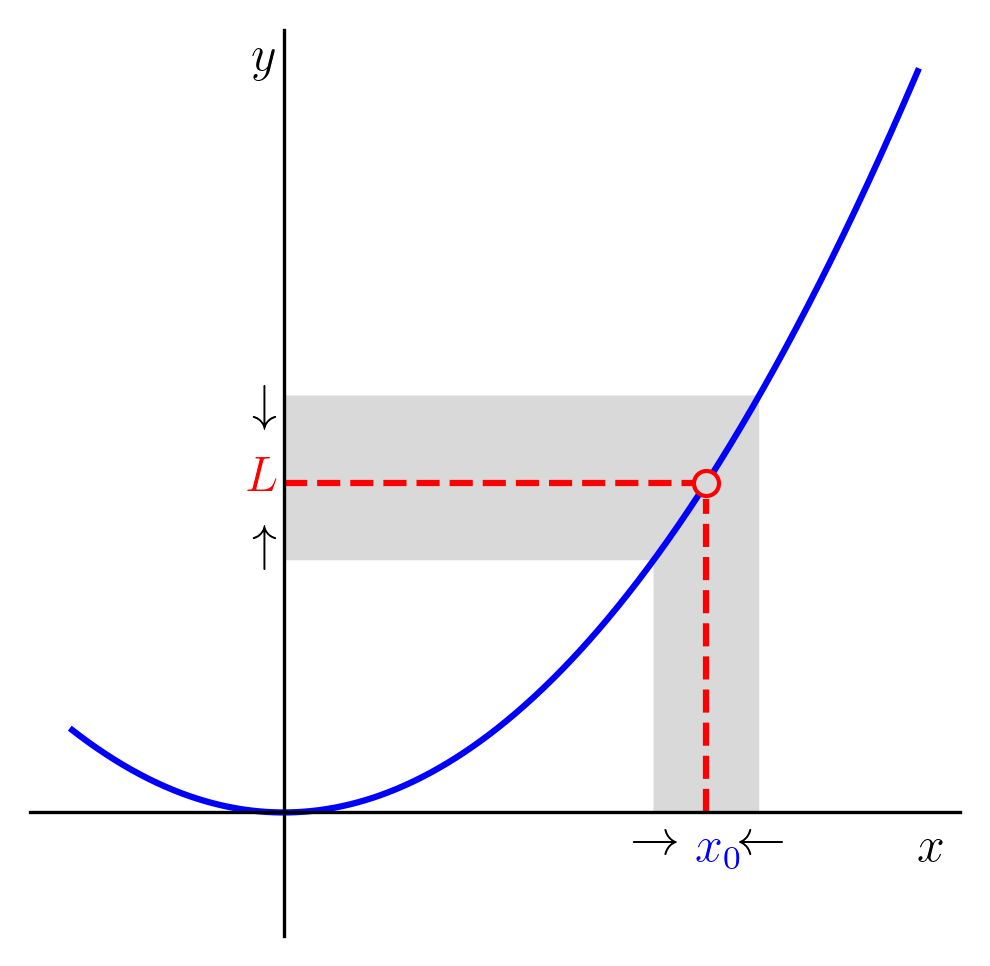
\includegraphics[width=4in]{./cap_lim/dados/fig_lim/fig.png}
  \caption{Noção de limite de uma função.}
  \label{fig:lim}
\end{figure}

\begin{ex}\label{ex:lim0}
  Consideremos a função
  \begin{equation}
    f(x) = \frac{(x^2-1)(x-2)}{(x-1)(x-2)}.
  \end{equation}
  Na Figura \ref{fig:ex_lim0}, temos um esboço do gráfico desta função.

  \begin{figure}[H]
    \centering
    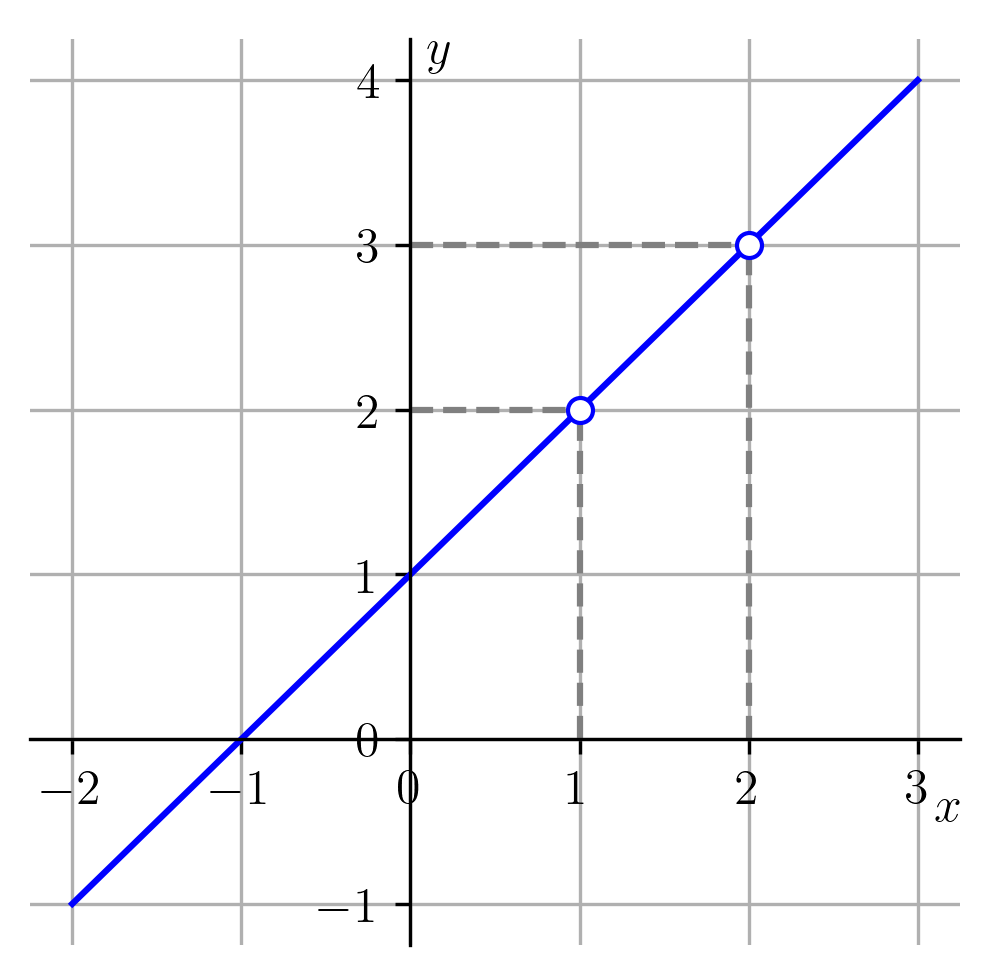
\includegraphics[width=4in]{./cap_lim/dados/fig_ex_lim0/fig.png}
    \caption{Gráfico da função $f(x)$ dada no Exemplo \ref{ex:lim0}.}
    \label{fig:ex_lim0}
  \end{figure}


  Vejamos os seguintes casos:
  \begin{itemize}
  \item $\displaystyle \lim_{x\to 0} f(x) = 1 = f(0)$.
    
    \begin{tabular}{r|ccc|c|ccc}
      $x$ & $-0,01$ & $-0,001$ & $-0,0001$ & $\rightarrow 0 \leftarrow$ & $0,0001$ & $0,001$ & $0,01$\\\hline
      $f(x)$ & $0,99$ & $0,999$ & $0,9999$ & $\rightarrow 1 \leftarrow$ & $1,0001$ & $1,001$ & $1,01$
    \end{tabular}

    \ifispython
    Com o {\python}+{\sympy}, podemos computar este limite com o comando
    \begin{lstlisting}
      >>> from sympy import *
      >>> x = Symbol('x')
      >>> limit((x**2-1)*(x-2)/((x-1)*(x-2))), x, 0)
      >>> 1
    \end{lstlisting}
    \fi
  \item $\displaystyle \lim_{x\to 1} f(x) = 2$, embora $f(1)$ não esteja definido.
    
    \begin{tabular}{r|ccc|c|ccc}
      $x$ & $0,9$ & $0,99$ & $0,999$ & $\rightarrow 1 \leftarrow$ & $1,0001$ & $1,001$ & $1,01$\\\hline
      $f(x)$ & $1,9$ & $1,99$ & $1,999$ & $\rightarrow 2 \leftarrow$ & $2,0001$ & $2,001$ & $2,01$
    \end{tabular}
  \item $\displaystyle \lim_{x\to 2} f(x) = 3$, embora $f(2)$ também não esteja definido. Verifique!
  \end{itemize}
\end{ex}

\subsection{Limites da função constante e da função identidade}\label{sslfc}
\badgeYouTube{\_7YiqVx8e8M}

Da noção de limite, podemos inferir que
\begin{equation}
  \lim_{x\to x_0} k = k,
\end{equation}
seja qual for a constante $k$. Veja a Figura \ref{fig:lim_funk}.

\begin{figure}[H]
  \centering
  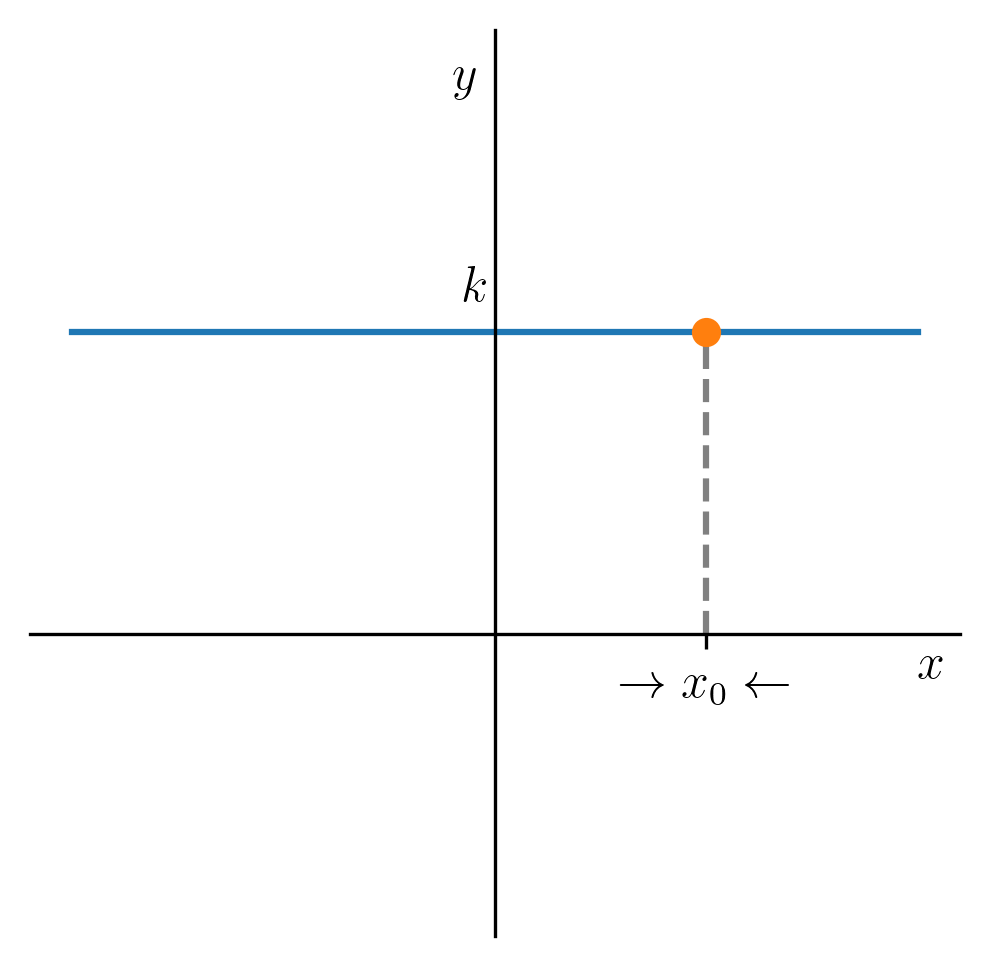
\includegraphics[width=4in]{./cap_lim/dados/fig_lim_funk/fig.png}
  \caption{Limite de função constante $f(x) = k$.}
  \label{fig:lim_funk}
\end{figure}

\begin{ex}
  Vejamos os seguintes casos:
  \begin{enumerate}[a)]
  \item $\displaystyle \lim_{x\to -1} 1 = 1$
    \ifispython
    No {\python}, podemos computar este limite com os seguintes comandos.
    \begin{lstlisting}
      >>> from sympy import *
      >>> x = Symbol("x")
      >>> limit(1, x, -1)
      >>> 1
    \end{lstlisting}
    \fi
  \item $\displaystyle \lim_{x\to 2} -3 = -3$
  \item $\displaystyle \lim_{x\to \pi} \left(\sqrt{2} - e\right) = \sqrt{2}-e$
  \end{enumerate}
\end{ex}

Também da noção de limites, podemos inferir que
\begin{equation}
  \lim_{x\to x_0} x = x_0,
\end{equation}
seja qual for o ponto $x_0$. Vejamos a Figura \ref{fig:lim_funid}.

\begin{figure}[H]
  \centering
  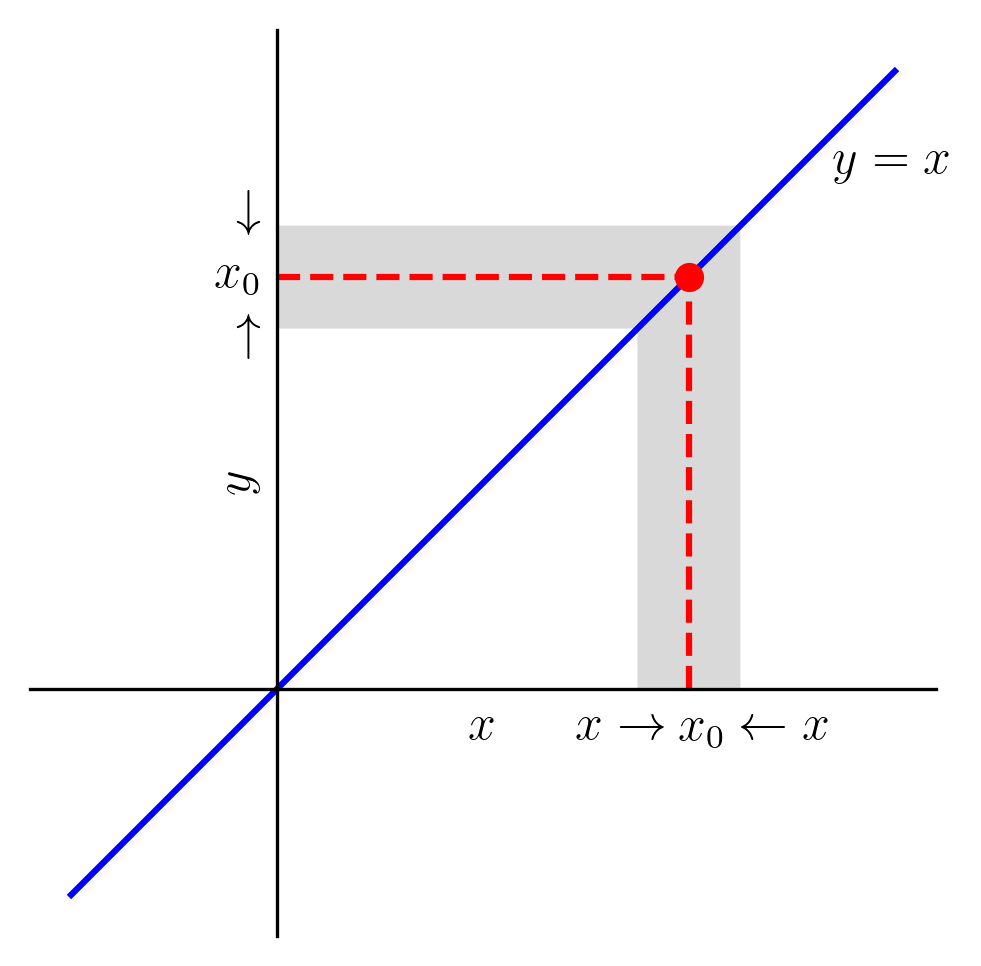
\includegraphics[width=4in]{./cap_lim/dados/fig_lim_funid/fig.png}
  \caption{Limite da função identidade $f(x)=x$.}
  \label{fig:lim_funid}
\end{figure}

\begin{ex}
  Vejamos os seguintes casos:
  \begin{enumerate}[a)]
  \item $\displaystyle \lim_{x\to -1} x = -1$
  \item $\displaystyle \lim_{x\to 2} x = 2$
  \item $\displaystyle \lim_{x\to \pi} x = \pi$
  \end{enumerate}
    \ifispython
    Com o {\python}+{\sympy}, podemos computar o limite do item a) com os seguintes comandos
    \begin{lstlisting}
      >>> from sympy import *
      >>> x = Symbol("x")
      >>> limit(x, x, -1)
      -1
    \end{lstlisting}
    Compute os outros itens e verifique os resultados!
    \fi
\end{ex}

\subsection{Exercícios resolvidos}

% \begin{flushright}
%   [Vídeo] | [Áudio] | \href{https://phkonzen.github.io/notas/contato.html}{[Contatar]}
% \end{flushright}

\begin{exeresol}
  Estime o valor do limite
  \begin{equation}
    \lim_{x\to 1} e^x.
  \end{equation}
\end{exeresol}
\begin{resol}
  Da noção de limite, podemos buscar inferir o limite de uma função em um ponto $x_0$, computando seus valores próximos deste ponto. Por exemplo, construímos a seguinte tabela:
  
  \begin{tabular}{r|ccc|c|ccc}
    $x$ & $0,9$ & $0,99$ & $0,999$ & $\rightarrow 1 \leftarrow$ & $1,0001$ & $1,001$ & $1,01$\\\hline
    $f(x)$ & $2,460$ & $2,691$ & $2,716$ & $\rightarrow 2,72 \leftarrow$ & $2,719$ & $2,721$ & $2,746$
  \end{tabular}
  
  Com isso, inferimos que
  \begin{equation}
    \lim_{x\to 1} e^x \approx 2,72.
  \end{equation}
  Mais adiante, veremos que $\lim_{x\to 1} e^x = e \approx 2,718281828459045 ...$.
  
  \ifispython
  Verifique usando {\python}+{\sympy}!
  \fi
\end{resol}

\begin{exeresol}
  Considere que uma dada função $f$ tenha o seguinte esboço de gráfico:

  \begin{center}
    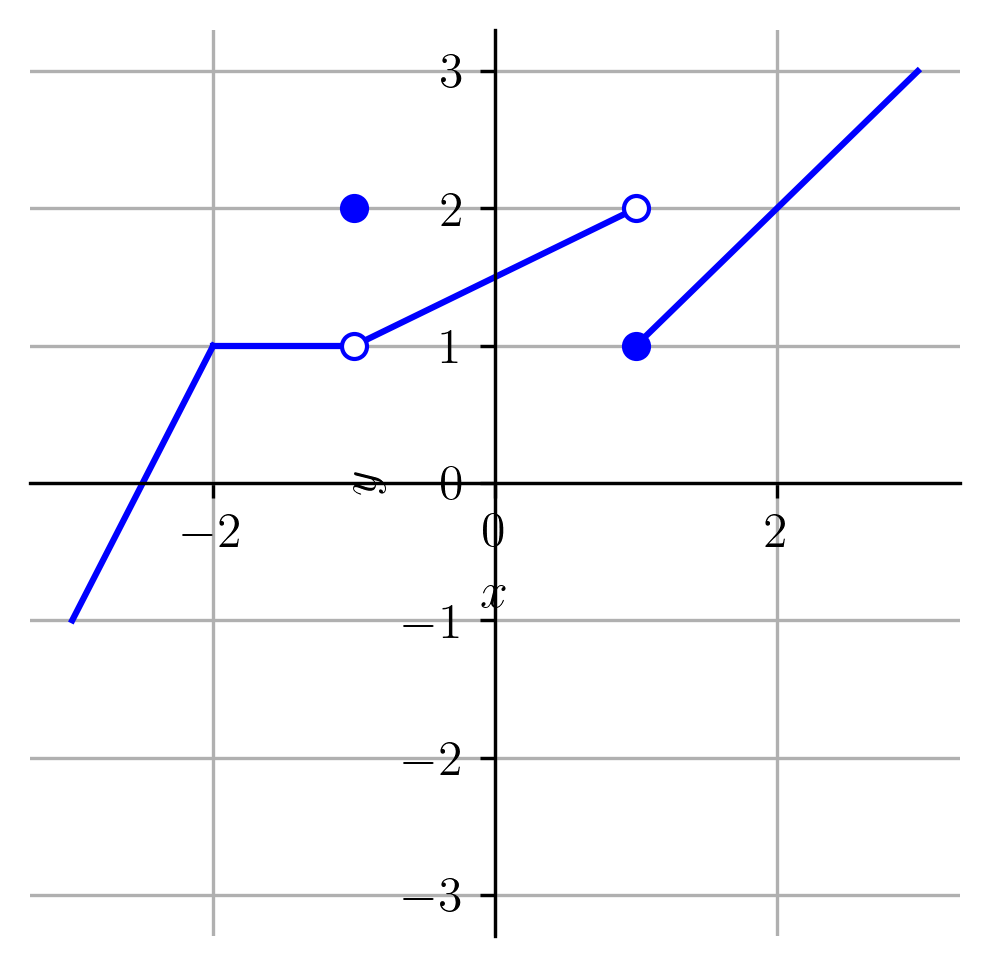
\includegraphics[width=4in]{./cap_lim/dados/fig_exeresol_nocaolim/fig.png}
  \end{center}

  Então, infira o valores de
  \begin{enumerate}[a)]
  \item $\displaystyle \lim_{x\to -2} f(x)$
  \item $\displaystyle \lim_{x\to -1} f(x)$
  \item $\displaystyle \lim_{x\to 1} f(x)$
  \end{enumerate}
\end{exeresol}
\begin{resol}
  \begin{enumerate}[a)]
  \item $\displaystyle \lim_{x\to -2} f(x)$

    Para valores suficientemente próximos de $-2$ e a direita de $-2$ (i.e. $x>-2$), podemos observar que $f(x)=1$. Para tais valores de $x$ a esquerda de $-2$ (i.e. $x<-2$), vemos que os valores de $f(x)$ tornam-se próximos de $1$. Isto é, temos que os valores de $f(x)$ podemos ser tomados arbitrariamente próximos de $L=1$, se tomarmos $x$ suficientemente próximo de $-2$. Concluímos que
    \begin{equation}
      \lim_{x\to -2} = 1.
    \end{equation}

  \item $\displaystyle \lim_{x\to -1} f(x)$

    Mesmo sendo $f(-1)=2$, observamos que os valores de $f(x)$ podem ser tomados arbitrariamente próximos de $1$, se escolhemos valores de $x$ suficientemente próximos de $-1$. Logo,
    \begin{equation}
      \lim_{x\to -1} f(x) = 1.
    \end{equation}

    \item $\displaystyle \lim_{x\to 1} f(x)$

      Aqui, para valores de $x$ suficientemente próximos de $x_0=1$ e a esquerda ($x<1$), vemos que os valores de $f(x)$ são próximos de $L=2$. Entretanto, para valores de $x$ suficientemente próximos de $x_0=1$ e a direita ($x>1$), temos que os valores de $f(x)$ são próximos de $L=1$. Ou seja, não é possível escolher um valor $L$ tal que $f(x)$ esteja arbitrariamente próxima ao tomarmos $x$ suficientemente próximo de $x_0=1$, pois $L$ dependerá de $x$ estar a esquerda ou a direita de do ponto $x_0 = 1$. Concluímos que este limite não existe, e escrevemos
      \begin{equation}
        \not\exists\lim_{x\to 1} f(x).
      \end{equation}
  \end{enumerate}
\end{resol}

\subsection{Exercícios}


\begin{exer}\label{exer:limgraf}
  Considere que uma dada função $f$ tenha o seguinte esboço de gráfico:

  \begin{center}
    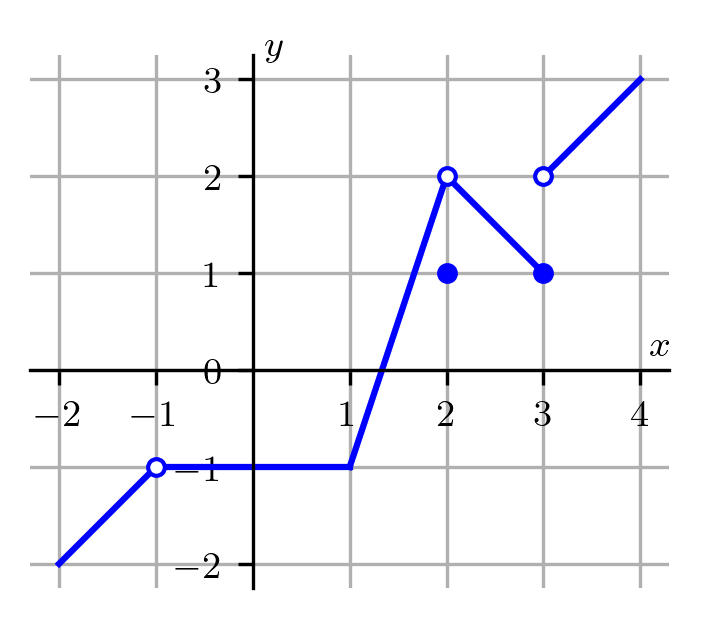
\includegraphics[width=4in]{./cap_lim/dados/fig_exer_limgraf/fig.png}
  \end{center}

  Forneça o valor dos seguintes limites:
  \begin{enumerate}[a)]
  \item $\displaystyle \lim_{x\to -1} f(x)$
  \item $\displaystyle \lim_{x\to 1} f(x)$
  \item $\displaystyle \lim_{x\to 2} f(x)$
  \item $\displaystyle \lim_{x\to 3} f(x)$
  \end{enumerate}
\end{exer}
\begin{resp}
  a)~$-1$; b)~$-1$; c)~$2$; d)~$\nexists$
\end{resp}

\begin{exer}
  Considerando a mesma função do exercício anterior (Exercício \ref{exer:limgraf}), forneça
  \begin{enumerate}
  \item $\displaystyle \lim_{x\to -\frac{3}{2}} f(x)$
  \item $\displaystyle \lim_{x\to 0} f(x)$
  \item $\displaystyle \lim_{x\to \frac{3}{4}} f(x)$
  \end{enumerate}
\end{exer}
\begin{resp}
  a)~$-\frac{3}{2}$; b)~$-1$; c)~$-1$
\end{resp}

\begin{exer}
  Forneça o valor dos seguintes limites:
  \begin{enumerate}[a)]
  \item $\displaystyle \lim_{x\to 2} 2$
  \item $\displaystyle \lim_{x\to -2} 2$
  \item $\displaystyle \lim_{x\to 2} -3$
  \item $\displaystyle \lim_{x\to e} \pi$
  \end{enumerate}
\end{exer}
\begin{resp}
  a)~2; b)~2; c)~-3; d)~$\pi$
\end{resp}

\begin{exer}
  Forneça o valor dos seguintes limites:
  \begin{enumerate}[a)]
  \item $\displaystyle \lim_{x\to 2} x$
  \item $\displaystyle \lim_{x\to -2} x$
  \item $\displaystyle \lim_{x\to -3} x$
  \item $\displaystyle \lim_{x\to e} x$
  \end{enumerate}
\end{exer}
\begin{resp}
  a)~2; b)~-2; c)~-3; d)~$e$
\end{resp}

\begin{exer}
  Com base na noção de limites, calcule:
  \begin{enumerate}[a)]
  \item $\displaystyle\lim_{x\to 1} |x|$
  \item $\displaystyle\lim_{x\to -1} |x|$
  \item $\displaystyle\lim_{x\to 10^{-10}} |x|$
  \end{enumerate}
\end{exer}
\begin{resp}
  a) $1$; b) $1$; c) $10^{-10}$
\end{resp}

\ifisbook
\subsubsection{Respostas}
\shipoutAnswer
\fi


\section{Regras para o cálculo de limites}\label{cap_lim_sec_regras}

\subsection{Regras de cálculo}
\badgeYouTube{chAoC7xoeYM}

Sejam dados os seguintes limites
\begin{align}
  & \lim_{x\to x_0} f(x) = L_1 \\
  & \lim_{x\to x_0} g(x) = L_2
\end{align}
com $x_0, L_1, L_2$ números reais. Então, valem as seguintes regras:
\begin{itemize}
\item Regra da multiplicação por um escalar:
  \begin{align}
    & \lim_{x\to x_0} k\cdot f(x) = k\cdot \lim_{x\to x_0} f(x)\\
    & \text{}\quad = k\cdot L_1,
  \end{align}
  para qualquer número real $k$.
\item Regra da soma/subtração:
  \begin{align}
    & \lim_{x\to x_0} f(x) \pm g(x) = \lim_{x\to x_0} f(x) \pm \lim_{x\to x_0} g(x) \\
    & \text{}\quad = L_1 \pm L_2
  \end{align}
\item Regra do produto:
  \begin{align}
    & \lim_{x\to x_0} f(x) \cdot g(x) = \lim_{x\to x_0} f(x) \cdot \lim_{x\to x_0} g(x) \\
    & \text{}\quad = L_1 \cdot L_2
  \end{align}
\item Regra do quociente:
  \begin{align}
    & \lim_{x\to x_0} \frac{f(x)}{g(x)} = \frac{\lim_{x\to x_0} f(x)}{\lim_{x\to x_0} g(x)} \\
    & \text{}\quad = \frac{L_1}{L_2},\qquad L_2\neq 0
  \end{align}
\item Regra da potenciação:
  \begin{align}
    & \lim_{x\to x_0} (f(x))^s = \left(\lim_{x\to x_0} f(x)\right)^s\\
    & \text{}\quad = L_1^s,\qquad L_1^s\in\mathbb{R}
  \end{align}
\end{itemize}

Podemos usar essas regras para calcularmos limites.

\begin{ex}
  Consideremos os seguintes casos:
  \begin{enumerate}[a)]
  \item $\displaystyle \lim_{x\to -1} 2x$
  \begin{align}
    & \lim_{x\to -1} 2x = 2\lim_{x\to -1} x\\
    & \text{}\quad = 2\cdot(-1) = -2
  \end{align}
  \ifispython
  Com o {\python}+{\sympy}, podemos computar este limite com
  \begin{lstlisting}
    >>> from sympy import *
    >>> x = Symbol("x")
    >>> limit(2*x, x, -1)
    -2
  \end{lstlisting}
  \fi
\item $\displaystyle \lim_{x\to 2} x^2 - 1$
  \begin{align}
    & \lim_{x\to 2} x^2 - 1 = \lim_{x\to 2} x^2 - \lim_{x\to 2} 1\\
    & \text{}\quad = \left(\lim_{x\to 2} x\right)^2 - 1\\
    & \text{}\quad = 2^2 - 1 = 3.
  \end{align}
  \ifispython
  Com o {\python}+{\sympy}, podemos computar este limite com os seguintes comandos.
  \begin{lstlisting}
    >>> from sympy import *
    >>> x = Symbol("x")
    >>> limit(x**2-1, x, 2)
    3
  \end{lstlisting}
  \fi
\item $\displaystyle \lim_{x\to 0} \sqrt{1-x^2}$.
  \begin{align}
    & \lim_{x\to 0} \sqrt{1-x^2} = \sqrt{\lim_{x\to 0} 1-x^2} \\
    & \text{}\quad = \sqrt{\lim_{x\to 0} 1 - \left(\lim_{x\to 0} x\right)^2} \\
    & \text{}\quad = \sqrt{1 - (0)^2} \\
    & \text{}\quad = 1.
  \end{align}
  \ifispython
  Com o {\python}+{\sympy}, podemos computar este limite com
  \begin{lstlisting}
    >>> from sympy import *
    >>> x = Symbol("x")
    >>> limit(sqrt(1-x**2), x, 0)
    1
  \end{lstlisting}
  \fi  
\item $\displaystyle \lim_{x\to 0} \frac{(x^2-1)(x-2)}{(x-1)(x-2)}$
  \begin{align}
    & \lim_{x\to 0} \frac{(x^2-1)(x-2)}{(x-1)(x-2)} = \frac{\displaystyle\lim_{x\to 0}\left[(x^2-1)\cdot(x-2)\right]}{\displaystyle\lim_{x\to 0} \left[(x-1)\cdot(x-2)\right]} \\
    & \text{}\quad = \frac{\displaystyle\lim_{x\to 0} (x^2-1)\cdot\lim_{x\to 0}(x-2)}{\displaystyle\lim_{x\to 0}(x-1)\cdot\lim_{x\to 0}(x-2)} \\
    & \text{}\quad = \frac{2}{2} = 1.
  \end{align}
  \end{enumerate}
\end{ex}

\begin{prop}\normalfont{(Limites de polinômios)}\label{prop:lim_poli}
  Se
  \begin{equation}
    p(x) = a_nx^n + a_{n-1}x^{n-1} + \cdots + a_0,
  \end{equation}
  então
  \begin{align}
    & \lim_{x\to b} p(x) = p(b) \\
    & \text{}\quad = a_nb^n + a_{n-1}b^{n-1} + \cdots + a_0,
  \end{align}
  para qualquer dado número real $b$.
\end{prop}
\begin{dem}
  Segue das regras da soma, da multiplicação por escalar e da potenciação.
  \begin{align}
    & \lim_{x\to b} p(x) = \lim_{x\to b} a_nx^n + a_{n-1}x^{n-1} + \cdots + a_0 \\
    & \text{}\quad = \lim_{x\to b} a_nx^n + \lim_{x\to b} a_{n-1}x^{n-1} + \cdots + \lim_{x\to b} a_0 \\
    & \text{}\quad = a_n\left(\lim_{x\to b} x\right)^n + a_{n-1}\left(\lim_{x\to b} x\right)^{n-1} + \cdots + a_0 \\
    & \text{}\quad = a_nb^n + a_{n-1}b^{n-1} + \cdots + a_0 = p(b).
  \end{align}
\end{dem}

\begin{ex}
  \begin{align}
    & \lim_{x\to \sqrt{2}} 2x^4 - 2x^2 + x = 2(\sqrt{2})^4 - 2(\sqrt{2})^2 + \sqrt{2} \\
    & \text{}\quad = 4+\sqrt{2}.
  \end{align}
  \ifispython
  Com o {\python}+{\sympy}, podemos computar este limite com os seguintes comandos.
  \begin{lstlisting}
    >>> from sympy import *
    >>> x = Symbol("x")
    >>> limit(2*x**4-2*x**2+x, x, sqrt(2))
    4 + sqrt(2)
  \end{lstlisting}
  \fi
\end{ex}

\begin{prop}\normalfont{(Limite de funções racionais)}
  Sejam $r(x) = p(x)/q(x)$ uma função racional e $b$ um número real tal que $q(b)\neq 0$. Então,
  \begin{equation}
    \lim_{x\to b} \frac{p(x)}{q(x)} = \frac{p(b)}{q(b)}.
  \end{equation}
\end{prop}
\begin{dem}
  Segue da regra do \emph{limite do quociente} e da Proposição \ref{prop:lim_poli}.
  \begin{align}
    & \lim_{x\to b} \frac{p(x)}{q(x)} = \frac{\displaystyle\lim_{x\to b} p(x)}{\displaystyle\lim_{x\to b} q(x)} \\
    & \quad = \frac{p(b)}{q(b)}.
  \end{align}
\end{dem}

\begin{ex}
  \begin{align}
    & \lim_{x\to 0} \frac{(x^2-1)(x-2)}{(x-1)(x-2)} = \frac{(0^2-1)(0-2)}{(0-1)(0-2)} \\
    & \quad = \frac{2}{2} = 1.
  \end{align}
  \ifispython
  Com o {\python}+{\sympy}, podemos computar este limite com os comandos.
  \begin{lstlisting}
    >>> from sympy import *
    >>> x = Symbol("x")
    >>> limit((x**2-1)*(x-2)/((x-1)*(x-2)), x, 0)
    1
  \end{lstlisting}
  \fi
\end{ex}

\subsection{Indeterminação $0/0$}
\badgeYouTube{dW3CfM2JjKY}
% \begin{flushright}
%   \href{https://youtu.be/dW3CfM2JjKY}{[YouTube]} | \href{https://archive.org/details/video_20220701_1415}{[Vídeo]} | [Áudio] | \href{https://phkonzen.github.io/notas/contato.html}{[Contatar]}
% \end{flushright}

Quando $\displaystyle \lim_{x\to a} f(a)=0$ e $\displaystyle \lim_{x\to a} g(a)=0$, dizemos que
\begin{equation}
  \lim_{x\to a} \frac{f(x)}{g(x)}
\end{equation}
é uma {\bf indeterminação do tipo $0/0$}. Em vários destes casos, podemos calcular o limite eliminando o fator em comum $(x-a)$.

\begin{ex}
  \begin{align}
    & \lim_{x\to 2}\frac{(x^2-1)\cancel{(x-2)}}{(x-1)\cancel{(x-2)}} = \lim_{x\to 2} \frac{x^2-1}{x-1} \\
    & \quad = \frac{2^2-1}{2-1} = 3.
  \end{align}
  \ifispython
  Com o {\python}+{\sympy}, podemos computar o limite acima com os seguintes comandos.
  \begin{lstlisting}
    >>> from sympy import *
    >>> x = Symbol("x")
    >>> limit((x**2-1)*(x-2)/((x-1)*(x-2)), x, 2)
    3
  \end{lstlisting}
  \fi
\end{ex}

Quando o fator em comum não aparece explicitamente, podemos tentar trabalhar algebricamente de forma a explicitá-lo.

\begin{ex}
  No caso do limite
  \begin{equation}
    \lim_{x\to 1} \frac{x^3-3x^2-x+3}{x^2+x-2}
  \end{equation}
  temos que o denominador $p(x) = x^3-3x^2-x+3$ se anula em $x=1$, assim como o denominador $q(x) = x^2+x-2$. Assim sendo, $(x-1)$ é um fator comum entre $p(x)$ e $q(x)$. Para explicitá-lo, calculamos
  \begin{align}
    & \frac{p(x)}{x-1} = \frac{x^3-3x^2-x+3}{x-1}\\
    & \quad = x^2-2x-3
  \end{align}
  e
  \begin{align}
    & \frac{q(x)}{x-1} = \frac{x^2+x-2}{x-1}\\
    & \quad = x+2.
  \end{align}
  \ifispython
  Com o {\python}+{\sympy}, podemos computar essas divisões com os seguintes comandos.
  \begin{lstlisting}
    >>> from sympy import *
    >>> x = Symbol("x")
    >>> simplify((x**3-3*x**2-x+3)/(x-1))
    x**2 - 2*x - 3
    >>> simplify((x**2+x-2)/(x-1))
    x + 2
  \end{lstlisting}
  \fi
  Realizadas as divisões, temos
  \begin{equation}
    p(x) = (x-1)(x^2-2x-3)
  \end{equation}
  e
  \begin{equation}
    q(x)=(x-1)(x+2).
  \end{equation}
  Com isso, segue que
  \begin{align}
    & \lim_{x\to 1} \frac{x^3-3x^2-x+3}{x^2+x-2} = \lim_{x\to 1} \frac{(x-1)(x^2-2x-3)}{(x-1)(x+2)} \\
    & \quad = \lim_{x\to 1} \frac{x^2-2x-3}{x+2} = -\frac{4}{3}.
  \end{align}
  \ifispython
  Use {\python}+{\sympy} para computar este limite!
  \fi
\end{ex}

\begin{ex}
  No caso de
  \begin{equation}
    \lim_{x\to 0} \frac{\sqrt{1-x}-1}{x}
  \end{equation}
  temos uma indeterminação do tipo $0/0$ envolvendo uma raiz. Neste caso, podemos calcular o limite usando de racionalização.
  \begin{align}
    & \lim_{x\to 0} \frac{\sqrt{1-x}-1}{x} = \lim_{x\to 0} \frac{\sqrt{1-x}-1}{x}\frac{\sqrt{1-x}+1}{\sqrt{1-x}+1} \\
    & \text{}\quad = \lim_{x\to 0} \frac{1-x-1}{x(\sqrt{1-x}+1)} \\
    & \text{}\quad - \lim_{x\to 0} \frac{-x}{x(\sqrt{1-x}+1)} \\
    & \text{}\quad = \lim_{x\to 0} \frac{-1}{\sqrt{1-x}+1} = -\frac{1}{2}.
  \end{align}
  \ifispython
  Verifique computando com o {\python}+{\sympy}. 
  \fi
\end{ex}

\subsection{Exercícios resolvidos}

% \begin{flushright}
%   [Vídeo] | [Áudio] | \href{https://phkonzen.github.io/notas/contato.html}{[Contatar]}
% \end{flushright}

\begin{exeresol}
  Calcule
  \begin{equation}
    \lim_{x\to -1} \frac{x - x^2}{\sqrt{x^2+3}}.
  \end{equation}
\end{exeresol}
\begin{resol}
  Usando das propriedades de limites, calculamos
  \begin{align}
    & \lim_{x\to -1} \frac{x-x^2}{\sqrt{x^2+3}} = \frac{\displaystyle\lim_{x\to -1} x-x^2}{\displaystyle\lim_{x\to -1} \sqrt{x^2+3}} \\
    & \text{}\quad = \frac{-1-(-1)^2}{\displaystyle\sqrt{\lim_{x\to -1} x^2+3}} \\
    & \text{}\quad = \frac{-2}{\sqrt{4}} = -1.
  \end{align}
\end{resol}

\begin{exeresol}
  Assumindo que o $\lim_{x\to 2} f(x) = L$ e que
  \begin{equation}
    \lim_{x\to 2} \frac{f(x)-2}{x+2} = 1,
  \end{equation}
  forneça o valor de $L$.
\end{exeresol}
\begin{resol}
  Das propriedades de limites, temos
  \begin{align}
    & \lim_{x\to 2} \frac{f(x)-2}{x+2} = 1 \\
    & \frac{\displaystyle\lim_{x\to 2} f(x)-2}{\displaystyle\lim_{x\to 2} x+2} = 1 \\
    & \frac{\lim_{x\to 2} f(x) - \lim_{x\to 2} 2}{2+2} = 1 \\
    & \frac{L-2}{4} = 1\\
    & L-2 = 4\\
    & L = 6.
  \end{align}
\end{resol}


\begin{exeresol}
  Calcule
  \begin{equation}
    \lim_{x\to -1} \frac{x+1}{2-\sqrt{x^2+3}}.
  \end{equation}
\end{exeresol}
\begin{resol}
  Neste caso, não podemos usar a regra do quociente, pois
  \begin{equation}
    \lim_{x\to -1} 2-\sqrt{x^2+3} = 0.
  \end{equation}
  Agora, como também temos
  \begin{equation}
    \lim_{x\to -1} x+1 = 0,
  \end{equation}
  concluímos se tratar de uma indeterminação $0/0$. Por racionalização, obtemos
  \begin{align}
    & \lim_{x\to -1} \frac{x+1}{2-\sqrt{x^2+3}} = \lim_{x\to -1} \frac{x+1}{2-\sqrt{x^2+3}}\frac{2+\sqrt{x^2+3}}{2+\sqrt{x^2+3}} \\
    & \text{}\quad = \lim_{x\to -1} \frac{(x+1)(2+\sqrt{x^2+3})}{4 - (x^2+3)} \\
    & \text{}\quad = \lim_{x\to -1} \frac{(x+1)(2+\sqrt{x^2+3})}{1-x^2} \\
    & \text{}\quad = \lim_{x\to -1} \frac{(x+1)(2+\sqrt{x^2+3})}{(1+x)(1-x)} \\
    & \text{}\quad = \lim_{x\to -1} \frac{2+\sqrt{x^2+3}}{1-x} \\
    & \text{}\quad = \frac{4}{2} = 2.
  \end{align}
\end{resol}

\subsection{Exercícios}

\begin{exer}
  Sabendo que
  \begin{equation}
    \lim_{x\to -2} f(x) = 2,
  \end{equation}
  calcule:
  \begin{enumerate}[a)]
  \item $\displaystyle \lim_{x\to -2} 2\cdot f(x)$.
  \item $\displaystyle \lim_{x\to -2} \pi\cdot f(x)$.
  \item $\displaystyle \lim_{x\to -2} -e^{\sqrt{2}}\cdot f(x)$.
  \end{enumerate}
\end{exer}
\begin{resp}
  a)~$4$; b)~$2\pi$; c)~$-2e^{\sqrt{2}}$
\end{resp}

\begin{exer}
  Considerando que
  \begin{equation}
    \lim_{x\to 3} f(x) = -2
  \end{equation}
  e
  \begin{equation}
    \lim_{x\to 3} g(x) = \frac{1}{2},
  \end{equation}
  calcule:
  \begin{enumerate}[a)]
  \item $\displaystyle\lim_{x\to 3} f(x)+g(x)$
  \item $\displaystyle\lim_{x\to 3} g(x)-f(x)$
  \item $\displaystyle\lim_{x\to 3} f(x)-2g(x)$
  \end{enumerate}
\end{exer}
\begin{resp}
  a)~$-3/2$; b)~$5/2$; c)~$-3$
\end{resp}

\begin{exer}
  Considerando que
  \begin{equation}
    \lim_{x\to 0} f(x) = 3
  \end{equation}
  e
  \begin{equation}
    \lim_{x\to 0} g(x) = -2,
  \end{equation}
  calcule:
  \begin{enumerate}[a)]
  \item $\displaystyle\lim_{x\to 0} f(x)\cdot g(x)$
  \item $\displaystyle\lim_{x\to 0} g(x)\cdot (\frac{1}{2}\cdot f(x))$
  \end{enumerate}
\end{exer}
\begin{resp}
  a)~$-6$; b)~$-3$;
\end{resp}

\begin{exer}
  Considerando que
  \begin{equation}
    \lim_{x\to 0} f(x) = -2
  \end{equation}
  e
  \begin{equation}
    \lim_{x\to 0} g(x) = -3,
  \end{equation}
  calcule:
  \begin{enumerate}[a)]
  \item $\displaystyle\lim_{x\to 0} \frac{f(x)}{g(x)}$
  \item $\displaystyle\lim_{x\to 0} \frac{g(x)}{2f(x)}$
  \end{enumerate}
\end{exer}
\begin{resp}
  a)~$2/3$; b)~$3/4$;
\end{resp}

\begin{exer}
  Considerando que
  \begin{equation}
    \lim_{x\to -1} f(x) = -1
  \end{equation}
  e
  \begin{equation}
    \lim_{x\to -1} g(x) = 4,
  \end{equation}
  calcule:
  \begin{enumerate}[a)]
  \item $\displaystyle\lim_{x\to -1} \sqrt{g(x)}$
  \item $\displaystyle\lim_{x\to -1} \sqrt[3]{f(x)}$
  \item $\displaystyle\lim_{x\to -1} (f(x))^{\frac{4}{3}}$
  \end{enumerate}
\end{exer}
\begin{resp}
  a)~$2$; b)~$-1$; c)~$1$
\end{resp}

\begin{exer}
  Calcule os limites:
  \begin{enumerate}[a)]
  \item $\displaystyle\lim_{x\to -2} -3x$
  \item $\displaystyle\lim_{x\to -2} x^2-3x$
  \item $\displaystyle\lim_{x\to -2} x^2-3x+\sqrt{x^2}$
  \end{enumerate}
\end{exer}
\begin{resp}
  a)~$6$; b)~$10$; c)~$12$
\end{resp}

\begin{exer}
  Calcule os limites:
  \begin{enumerate}[a)]
  \item $\displaystyle\lim_{x\to -1} \frac{x}{x-1}$
  \item $\displaystyle\lim_{x\to -1} \frac{x^2+x-2}{x^2-3x+2}$
  \end{enumerate}
\end{exer}
\begin{resp}
  a)~$1/2$; b)~$-1/3$;
\end{resp}

\begin{exer}
  Calcule os limites:
  \begin{enumerate}[a)]
  \item $\displaystyle\lim_{x\to 1} \frac{x^2-1}{x-1}$
  \item $\displaystyle\lim_{x\to -1} \frac{x^2-1}{2x+2}$
  \item $\displaystyle\lim_{x\to 1} \frac{x^2+x-2}{x^2-3x+2}$
  \end{enumerate}
\end{exer}
\begin{resp}
  a)~$2$; b)~$-1$; c)~$-3$;
\end{resp}

\begin{exer}
  Calcule o limite
  \begin{equation}
    \lim_{x\to 6} \frac{2-\sqrt{x-2}}{x-6}.
  \end{equation}
\end{exer}
\begin{resp}
  $-1/4$
\end{resp}

\begin{exer}
  Diga se é verdadeira ou falsa a seguinte afirmação. Se existem
  \begin{align}
    & \lim_{x\to 1} f(x) = L \\
    & \lim_{x\to -1} g(x) = M
  \end{align}
  então
  \begin{equation}
    \lim_{x\to 1} f(x) + g(x) = L + M.
  \end{equation}
  Justifique sua resposta.
\end{exer}
\begin{resp}
  Falso. Construa um contraexemplo para mostrar que a afirmação não é verdadeira. 
\end{resp}

\ifisbook
\subsubsection{Respostas}
\shipoutAnswer
\fi


\section{Limites laterais}\label{cap_lim_sec_lateral}
\badgeYouTube{BFJPIejdyZM}

Seja dada uma função $f$ definida para todo $x$ em um intervalo aberto $(a, x_0)$. O {\bf limite lateral à esquerda} de $f$ no ponto $x_0$ é denotado por
\begin{equation}
  \lim_{x\to {\color{red}x_0^-}} f(x)
\end{equation}
e é computado tendo em vista a tendência da função apenas para pontos $x<x_0$. Em outras palavras, o
\begin{equation}
  \lim_{x\to x_0^-} f(x) = L
\end{equation}
quando $f(x)$ é arbitrariamente próximo de $L$, para todo $x<x_0$ suficientemente próximo de $x_0$. Veja a Figura~\ref{fig:lim_esq}.

\begin{figure}[H]
  \centering
  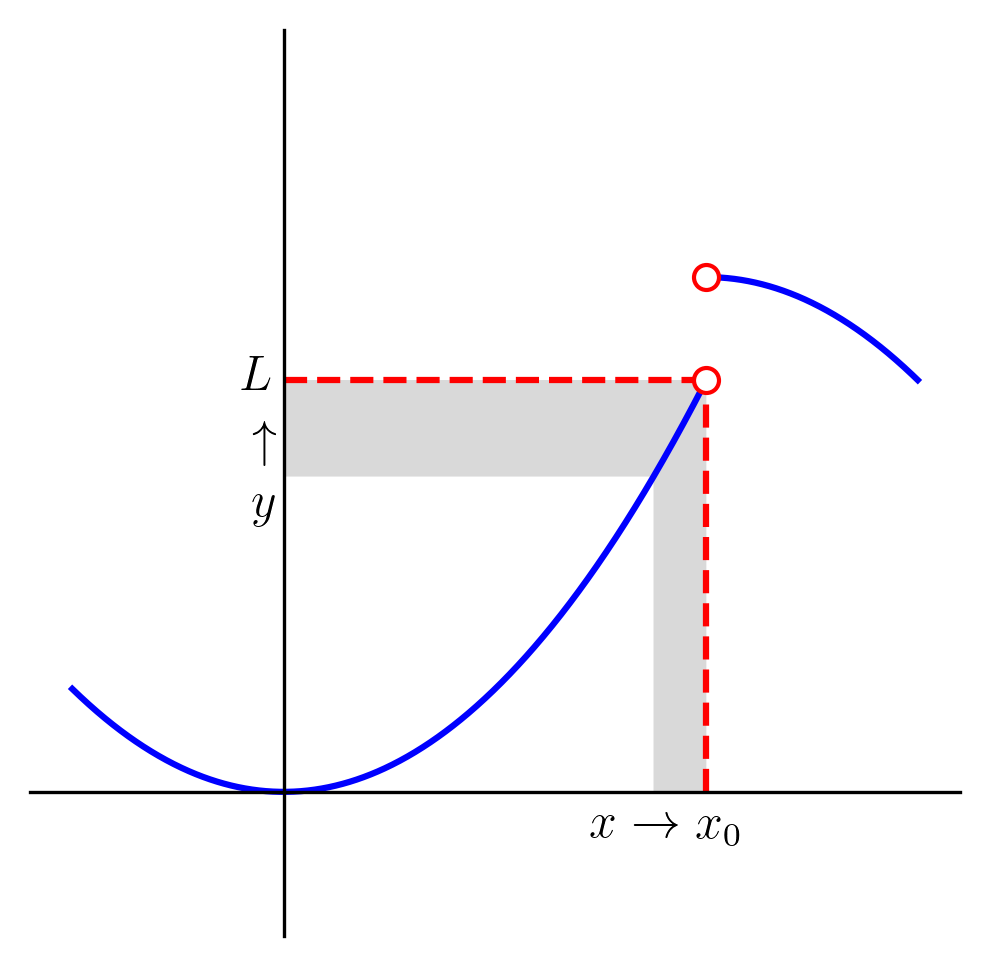
\includegraphics[width=4in]{./cap_lim/dados/fig_lim_esq/fig.png}
  \caption{Limite lateral à esquerda.}
  \label{fig:lim_esq}
\end{figure}

Para uma função $f$ definida para todo $x$ em um intervalo aberto $(x_0, b)$, o {\bf limite lateral à direita} de $f$ no ponto $x_0$ é denotado por
\begin{equation}
  \lim_{x\to {\color{blue}x_0^+}} f(x)
\end{equation}
e é computado tendo em vista a tendência da função apenas para pontos $x>x_0$. Em outras palavras, temos
\begin{equation}
  \lim_{x\to x_0^+} f(x) = L,
\end{equation}
quando $f(x)$ é arbitrariamente próximo de $L$, para todo $x>x_0$ suficientemente próximo de $x_0$. Veja a Figura \ref{fig:lim_dir}.

\begin{figure}[H]
  \centering
  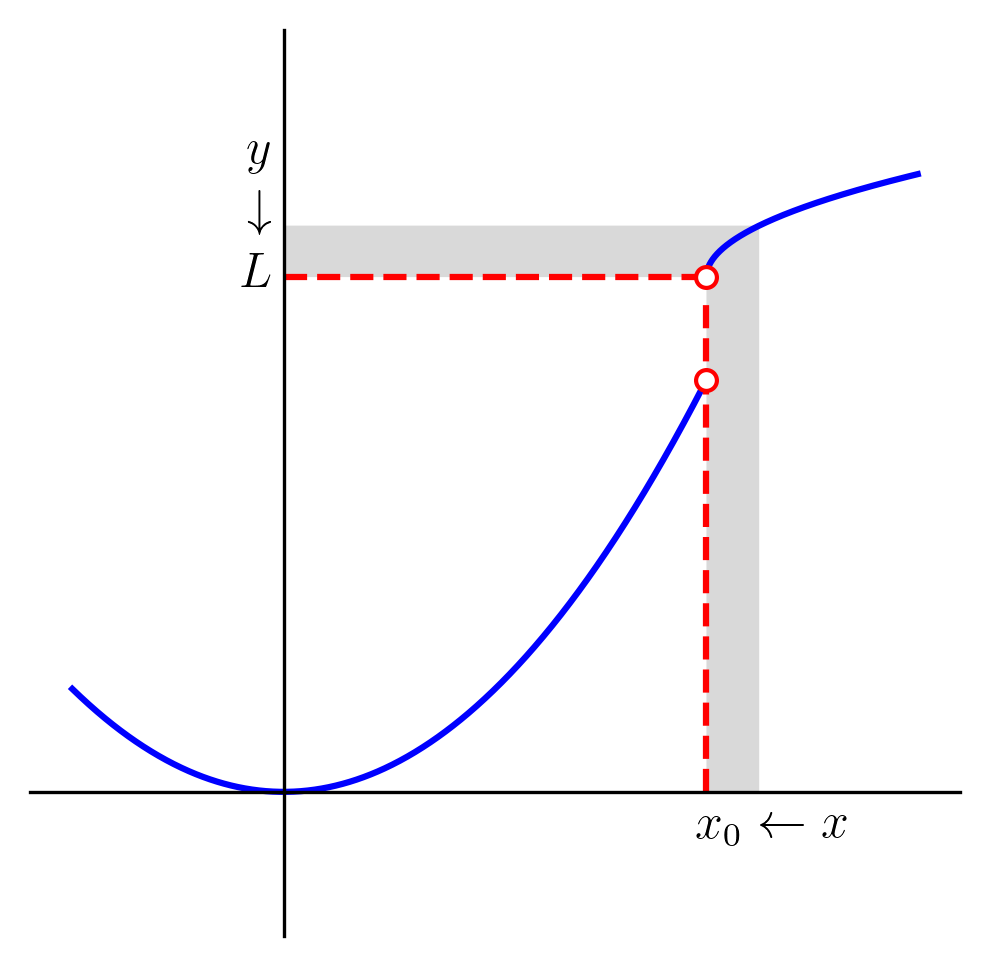
\includegraphics[width=4in]{./cap_lim/dados/fig_lim_dir/fig.png}
  \caption{Limite lateral à direita.}
  \label{fig:lim_dir}
\end{figure}

\begin{obs}
  Por inferência direta, temos
  \begin{equation}
    \lim_{x\to x_0^{\pm}} k = k
  \end{equation}
  e
  \begin{equation}
    \lim_{x\to x_0^{\pm}} x = x_0,
  \end{equation}
  onde $x_0$ e $k$ são quaisquer dados números reais.
\end{obs}

\begin{exer}\label{ex:lim_absx}
  Vamos calcular
  \begin{equation}
    \lim_{x\to 0^-} |x|.
  \end{equation}
  Por definição, temos
  \begin{equation}
    |x| := \left\{
      \begin{array}{ll}
        x &, x\geq 0,\\
        -x &, x< 0.
      \end{array}
    \right.
  \end{equation}
  Como estamos interessados no limite lateral à esquerda de $x=0$, trabalhamos com $x<0$ e, então
  \begin{align}
    & \lim_{x\to 0^-} |x| = \lim_{x\to 0^-} -x \\
    & \text{}\quad = -\lim_{x\to 0^-} x = 0.
  \end{align}
  
  Analogamente, calculamos
  \begin{equation}
    \lim_{x\to 0^+} |x| = \lim_{x\to 0^+} x = 0.
  \end{equation}
  Verifique!

  \ifispython
  Com o {\python}+{\sympy}, podemos computar os limites acima com os seguintes comandos.
  \begin{lstlisting}
    >>> from sympy import *
    >>> x = Symbol("x")
    >>> limit(abs(x), x, 0, '-')
    0
    >>> limit(abs(x), x, 0, '+')
    0
  \end{lstlisting}
  \fi
\end{exer}

\begin{teo}\label{teo:lim_existe}
  Existe o limite de uma dada função $f$ no ponto $x=x_0$ e
  \begin{equation}
    \lim_{x\to x_0} f(x) = L
  \end{equation}
  se, e somente se, existem e são iguais a $L$ os limites laterais à esquerda e à direita de $f$ no ponto $x=x_0$.
\end{teo}

\begin{exer}
  No exemplo anterior (Exemplo \ref{ex:lim_absx}), vimos que
  \begin{equation}
    \lim_{x\to 0^-} |x| = \lim_{x\to 0^+} |x| = 0.
  \end{equation}
  Logo, pelo teorema acima (Teorema \ref{teo:lim_existe}), podemos concluir que
  \begin{equation}
    \lim_{x\to 0} |x| = 0.
  \end{equation}
\end{exer}

\begin{exer}
  Vamos verificar a existência de
  \begin{equation}
    \lim_{x\to 0} \frac{|x|}{x}.
  \end{equation}
  Começamos pelo limite lateral à esquerda, temos
  \begin{align}
    & \lim_{x\to 0^-} \frac{|x|}{x} = \lim_{x\to 0^-} \frac{-x}{x} \\
    & \text{}\quad = \lim_{x\to 0^-} -1 = -1.
  \end{align}
  Agora, calculando o limite lateral à direta, obtemos
  \begin{align}
    & \lim_{x\to 0^+} \frac{|x|}{x} = \lim_{x\to 0^+} \frac{x}{x} \\
    & \text{}\quad = \lim_{x\to 0^+} 1 = 1.
  \end{align}
  Como os \emph{limites laterais} à esquerda e à direita \emph{são diferentes}, concluímos que \emph{não existe o limite} de $|x|/x$ no ponto $x=0$.

  \ifispython
  Com o {\python}+{\sympy}, por padrão o limite computado é sempre o limite lateral à direita. É por isso que o comando
  \begin{lstlisting}
    >>> from sympy import *
    >>> x = Symbol("x")
    >>> limit(abs(x)/x, x, 0)
    1
  \end{lstlisting}
  fornece o valor $1$ como saída. Compute os limites laterais e verifique com os resultados analíticos obtidos acima!
  \fi
\end{exer}

\begin{obs}
  As regras básicas para o cálculo de limites bilaterais são estendidas para limites laterais. I.e., se
  \begin{equation}
    \lim_{x\to x_0^{\pm}} f(x) = L_1
  \end{equation}
  e
  \begin{equation}
    \lim_{x\to x_0^{\pm}} g(x) = L_2,
  \end{equation}
  então valem a:
  \begin{itemize}
\item regra da multiplicação por um escalar:
  \begin{equation}
    \lim_{x\to x_0^{\pm}} kf(x) = k\lim_{x\to x_0^{\pm}} f(x) = kL_1,
  \end{equation}
  para qualquer número real $k$.
\item regra da soma/subtração:
  \begin{align}
    & \lim_{x\to x_0^{\pm}} f(x) \pm g(x) = \lim_{x\to x_0^{\pm}} f(x) \pm \lim_{x\to x_0^{\pm}} g(x) \\
    & \text{}\quad = L_1 + L_2
  \end{align}
\item regra do produto:
  \begin{align}
    & \lim_{x\to x_0^\pm} f(x) \cdot g(x) = \lim_{x\to x_0^\pm} f(x) \cdot \lim_{x\to x_0^\pm} g(x) \\
    & \text{}\quad = L_1 \cdot L_2
  \end{align}
\item regra do quociente:
  \begin{align}
    & \lim_{x\to x_0^\pm} \frac{f(x)}{g(x)} = \frac{\lim_{x\to x_0^\pm} f(x)}{\lim_{x\to x_0^\pm} g(x)} \\
    & \text{}\quad = \frac{L_1}{L_2},
  \end{align}
  desde que $L_2\neq 0$.
\item regra da potenciação:
  \begin{align}
    & \lim_{x\to x_0^\pm} (f(x))^s = \left(\lim_{x\to x_0^\pm} f(x) \right)^s \\
    & \text{}\quad = L_1^s,
  \end{align}
  se, adicionalmente, $L_1^s$ é um número real.
\end{itemize}
\end{obs}

\subsection{Exercícios resolvidos}

\begin{exeresol}
  Considere que uma dada função $f$ tenha o seguinte esboço de gráfico:

  \begin{center}
    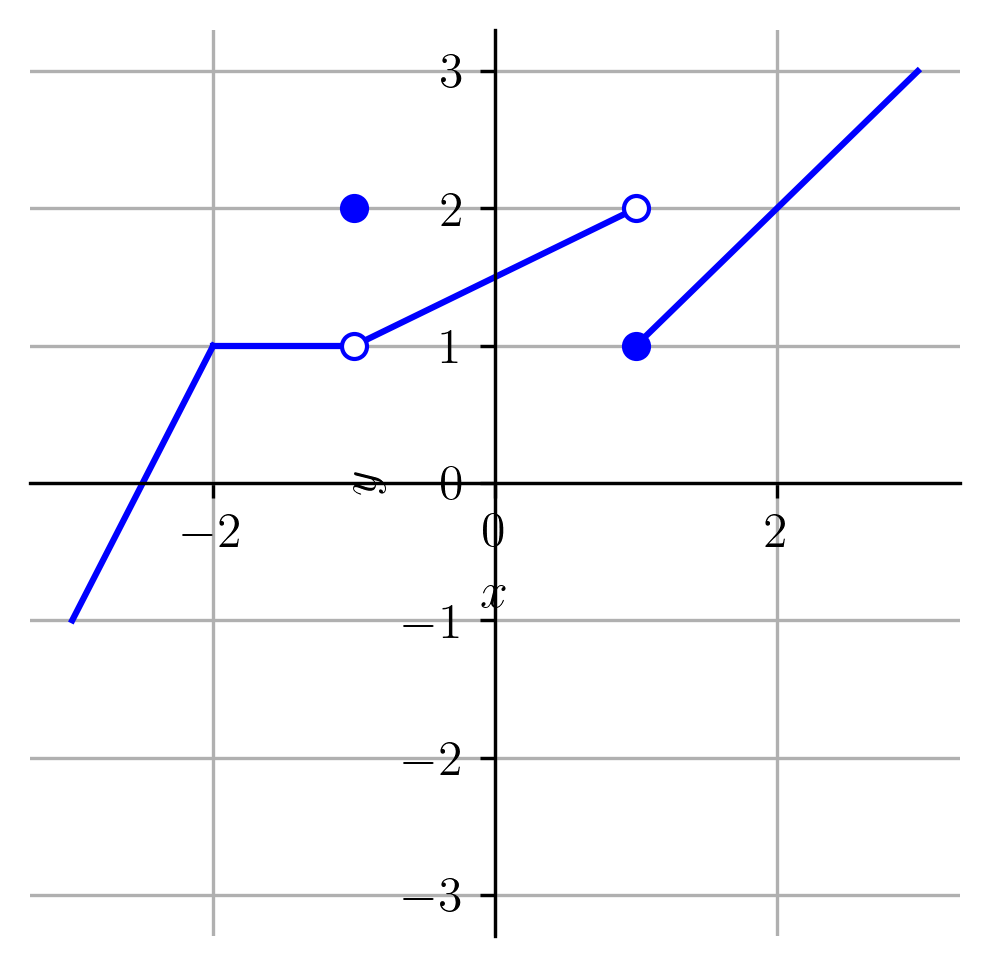
\includegraphics[width=4in]{./cap_lim/dados/fig_exeresol_nocaolim/fig.png}
  \end{center}

  Então, infira o valores de
  \begin{enumerate}[a)]
  \item $\displaystyle \lim_{x\to -2^-} f(x)$
  \item $\displaystyle \lim_{x\to -1^+} f(x)$
  \item $\displaystyle \lim_{x\to 1^-} f(x)$
  \item $\displaystyle \lim_{x\to 1^+} f(x)$
  \item $\displaystyle \lim_{x\to 1} f(x)$
  \end{enumerate}
\end{exeresol}
\begin{resol}
  \begin{enumerate}[a)]
  \item $\displaystyle \lim_{x\to -2^-} f(x)$

    Para valores $x<-2$ e suficientemente próximos de $-2$, podemos observar que $f(x)$ fica arbitrariamente próximo de $1$. Concluímos que
    \begin{equation}
      \lim_{x\to -2^-} = 1.
    \end{equation}

  \item $\displaystyle \lim_{x\to -1^+} f(x)$

    Mesmo sendo $f(-1)=2$, observamos que os valores de $f(x)$ podem ser tomados arbitrariamente próximos de $1$, se escolhemos valores de $x>-1$ e suficientemente próximos de $-1$. Logo,
    \begin{equation}
      \lim_{x\to -1^+} f(x) = 1.
    \end{equation}

  \item $\displaystyle \lim_{x\to 1^-} f(x)$

    Observamos que os valores de $f(x)$ podem ser tomados arbitrariamente próximos de $2$, se escolhemos valores de $x<1$ e suficientemente próximos de $1$. Logo,
    \begin{equation}
      \lim_{x\to 1^-} f(x) = 2.
    \end{equation}
    Notamos também que, neste caso, $f(x)$ não tende para $f(1)=1$ quando $x$ tende a $1$ pela esquerda.

  \item $\displaystyle \lim_{x\to 1^+} f(x)$

    Observamos que os valores de $f(x)$ podem ser tomados arbitrariamente próximos de $1$, se escolhemos valores de $x>1$ e suficientemente próximos de $1$. Logo,
    \begin{equation}
      \lim_{x\to 1^+} f(x) = 1.
    \end{equation}
    Aqui, $f(x)\to f(1)=1$ quando $x\to 1^+$.

    \item $\displaystyle \lim_{x\to 1} f(x)$

      Nos itens anteriores, vimos que
      \begin{equation}
        2 = \lim_{x\to 1^-} f(x) \neq \lim_{x\to 1^+} f(x) = 1.
      \end{equation}
      Logo, concluímos que este limite não existe, e escrevemos
      \begin{equation}
        \not\exists\lim_{x\to 1} f(x).
      \end{equation}
  \end{enumerate}
\end{resol}

\begin{exeresol}
  Calcule $\lim_{x\to -1} f(x)$ para
  \begin{equation}
    f(x) = \left\{
      \begin{array}{ll}
        (x+1)^2-1 &, x<-1,\\
        x &, x>-1.
      \end{array}
\right.
  \end{equation}
\end{exeresol}
\begin{resol}
  A função $f$ tem comportamentos distintos para valores à esquerda e à direita de $x_0=-1$. Portanto, para calcularmos $\lim_{x\to -1} f(x)$ precisamos calcular os limites laterais. Temos:
  \begin{align}
    & \lim_{x\to -1^-} f(x) = \lim_{x\to -1^-} (x+1)^2-1 \\
    & \text{}\quad = (-1+1)^2-1 = -1,
  \end{align}
  e
  \begin{align}
    & \lim_{x\to -1^+} f(x) = \lim_{x\to -1^+} x \\
    & \text{}\quad = -1.
  \end{align}
  Como ambos os limites laterais são iguais a $-1$, concluímos que
  \begin{equation}
    \lim_{x\to -1} f(x) = -1.
  \end{equation}
\end{resol}

\subsection{Exercícios}

\begin{exer}\label{exer:limgraf_lat}
  Considere que uma dada função $f$ tenha o seguinte esboço de gráfico:

  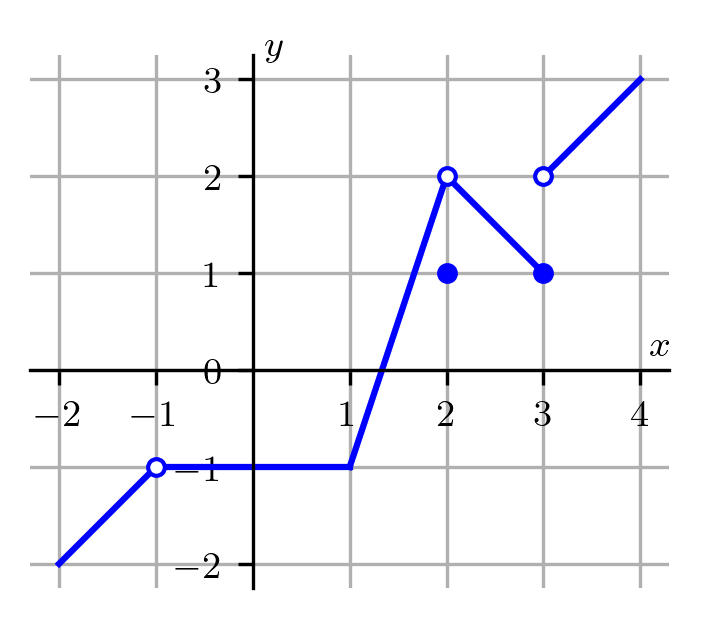
\includegraphics[width=4in]{./cap_lim/dados/fig_exer_limgraf/fig.png}

  Forneça o valor dos seguintes limites:
  \begin{enumerate}[a)]
  \item $\displaystyle \lim_{x\to 2^+} f(x)$
  \item $\displaystyle \lim_{x\to 2^-} f(x)$
  \item $\displaystyle \lim_{x\to 2} f(x)$
  \item $\displaystyle \lim_{x\to 3^+} f(x)$
  \item $\displaystyle \lim_{x\to 3^-} f(x)$
  \item $\displaystyle \lim_{x\to 3} f(x)$
  \end{enumerate}
\end{exer}
\begin{resp}
  a)~$2$; b)~$2$; c)~$2$; d)~$2$; e)~$1$; f)~$\nexists$
\end{resp}

\begin{exer}
  Sendo
  \begin{equation}
    f(x) = \left\{
      \begin{array}{ll}
        x^2+1 &, x\leq 1,\\
        2x &, x>1.
      \end{array}
    \right.
  \end{equation}
  calcule
  \begin{enumerate}[a)]
  \item $\displaystyle \lim_{x\to 1^-} f(x)$.
  \item $\displaystyle \lim_{x\to 1^+} f(x)$.
  \item $\displaystyle \lim_{x\to 1} f(x)$.
  \end{enumerate}
\end{exer}
\begin{resp}
  a)~$2$; b)~$2$; c)~$2$
\end{resp}

\begin{exer}
  Sendo
  \begin{equation}
    f(x) = \left\{
      \begin{array}{ll}
        x^2+1 &, x\leq 1,\\
        2x+1 &, x>1,
      \end{array}
    \right.
  \end{equation}
  calcule
  \begin{enumerate}[a)]
  \item $\displaystyle \lim_{x\to 1^-} f(x)$.
  \item $\displaystyle \lim_{x\to 1^+} f(x)$.
  \item $\displaystyle \lim_{x\to 1} f(x)$.
  \end{enumerate}
\end{exer}
\begin{resp}
  a)~$2$; b)~$3$; c)~$\nexists$
\end{resp}

\begin{exer}
  Calcule
  \begin{equation}
    \lim_{x\to 0^-} \frac{x}{2|x|}.
  \end{equation}
\end{exer}
\begin{resp}
  $-\frac{1}{2}$
\end{resp}

\begin{exer}
  Calcule
  \begin{equation}
    \lim_{x\to -1^+} \sqrt{1-x^2}.
  \end{equation}
  O que pode-se dizer sobre o limite à esquerda?
\end{exer}
\begin{resp}
  $0$; Não está definido, pois o domínio de $f(x)=\sqrt{1-x^2}$ é $[-1, 1]$.
\end{resp}

\begin{exer}
  Diga se é verdadeira ou falsa a seguinte afirmação. Se existem
  \begin{align}
    & \lim_{x\to 1^-} f(x) = L\\
    & \lim_{x\to 1^+} g(x) = M
  \end{align}
  então
  \begin{equation}
    \lim_{x\to 1^-} f(x) + g(x) = L + M.
  \end{equation}
  Justifique sua resposta.
\end{exer}
\begin{resp}
  Falso. Dica: construa um contraexemplo para mostrar que a afirmação não é verdadeira. 
\end{resp}

\ifisbook
\subsubsection{Respostas}
\shipoutAnswer
\fi


\section{Limites no infinito}\label{cap_lim_sec_liminf}
\badgeYouTube{Ni9afaabTws}

Limites no infinito descrevem a tendência de uma dada função $f(x)$ quando $x\to -\infty$ ou $x\to\infty$. Dizemos que o limite de $f(x)$ é $L$ quando $x$ tende a $-\infty$, se os valores de $f(x)$ são {\bf arbitrariamente próximos} de $L$ para todos os valores de $x$ {\bf suficientemente pequenos}. Neste caso, escrevemos
\begin{equation}
  \lim_{x\to -\infty} f(x) = L.
\end{equation}
Veja a Figura~\ref{fig:lim_x-infty}.

\begin{figure}[H]
  \centering
  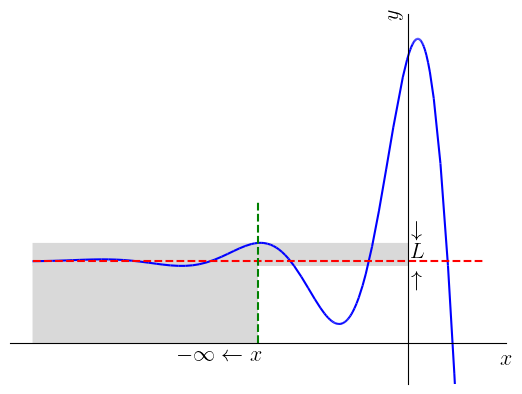
\includegraphics[width=0.7\textwidth]{./cap_lim/dados/fig_lim_x-infty/fig_lim_x-infty}
  \caption{Ilustração da noção de limite de uma função quando $x\to -\infty$.}
  \label{fig:lim_x-infty}
\end{figure}

Analogamente, dizemos que o limite de $f(x)$ é $L$ quando $x$ tende $\infty$, se os valores de $f(x)$ são {\bf arbitrariamente próximos} de $L$ para todos os valores de $x$ {\bf suficientemente grandes}. Neste caso, escrevemos
\begin{equation}
  \lim_{x\to \infty} f(x) = L.
\end{equation}
Veja a Figura \ref{fig:lim_x2infty}.

\begin{figure}[H]
  \centering
  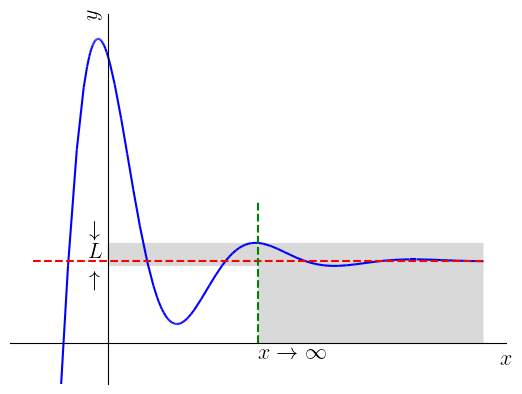
\includegraphics[width=0.7\textwidth]{./cap_lim/dados/fig_lim_x2infty/fig_lim_x2infty}
  \caption{Ilustração da noção de limite de uma função quando $x\to \infty$.}
  \label{fig:lim_x2infty}
\end{figure}


\begin{ex}
  Vamos inferir os limites de $f(x) = 1/x$ para $x\to -\infty$ e $x\to \infty$. A Figura \ref{fig:lim_xinf_1x} é um esboço do gráfico desta função.

\begin{figure}[H]
  \centering
  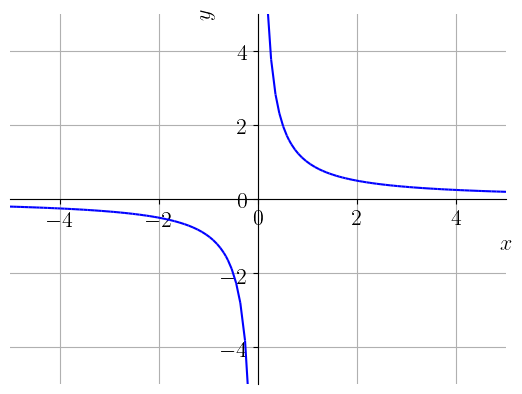
\includegraphics[width=0.7\textwidth]{./cap_lim/dados/fig_lim_xinf_1x/fig_lim_xinf_1x}
  \caption{Esboço do gráfico de $f(x) = 1/x$.}
  \label{fig:lim_xinf_1x}
\end{figure}

Observamos que quanto menores os valores de $x$, mais próximos de $0$ são os valores de $f(x)=1/x$. Daí, inferimos que
\begin{equation}
  \lim_{x\to -\infty} \frac{1}{x} = 0.
\end{equation}

Também, quanto maiores os valores de $x$, mais próximos de $0$ são os valores de $f(x)=1/x$. Com isso, podemos concluir que
\begin{equation}
  \lim_{x\to \infty} \frac{1}{x} = 0.
\end{equation}

\ifispython
Podemos computar estes limites com o {\python}+{\sympy}, usando os seguintes comandos:
\begin{lstlisting}
  >>> from sympy import *
  >>> x = Symbol("x")
  >>> limit(1/x, x, -oo)
  0
  >>> limit(1/x, x, oo)
  0
\end{lstlisting}
\fi
\end{ex}

\begin{obs}\normalfont{(Regras para o cálculo de limites no infinito)}\label{obs:lim_regras_xinf}
Supondo que $L$, $M$ e $k$ são números reais e
\begin{equation}
  \lim_{x\to \pm\infty} f(x) = L
\end{equation}
e
\begin{equation}
  \lim_{x\to\pm\infty}g(x) = M.
\end{equation}
Então, temos as seguintes regras para limites no infinito:
\begin{itemize}
\item Regra da multiplicação por escalar
  \begin{equation}
    \lim_{x\to\pm\infty} kf(x) = kL
  \end{equation}
\item Regra da soma/diferença
  \begin{equation}
    \lim_{x\to\pm\infty} (f(x)\pm g(x)) = L\pm M
  \end{equation}
\item Regra do produto
  \begin{equation}
    \lim_{x\to\pm\infty} f(x)g(x) = LM
  \end{equation}
\item Regra do quociente
  \begin{equation}
    \lim_{x\to\pm\infty} \frac{f(x)}{g(x)} = \frac{L}{M},\quad M\neq 0.
  \end{equation}
\item Regra da potenciação
  \begin{equation}
    \lim_{x\to\pm\infty} (f(x))^k = L^k,\text{ se } L^k\in\mathbb{R}.
  \end{equation}
\end{itemize}
\end{obs}

\begin{ex}
  \begin{align}
    & \lim_{x\to \infty} \frac{1}{x^2}+1 \\
    & \text{}\quad = \lim_{x\to \infty} \frac{1}{x^2} + \lim_{x\to \infty}1 \\
    &  \text{}\quad = \left(\lim_{x\to\infty} \frac{1}{x}\right)^2 + 1 \\
    & \text{}\quad = 0^2 + 1 = 1.
\end{align}
\end{ex}

\begin{ex}\label{ex:liminf_funracio}
  Consideramos o seguinte caso
  \begin{equation}
    \lim_{x\to \infty} \frac{x^3 - 2x + 1}{2 - 3x^3}.
  \end{equation}
  Observamos que não podemos usar a regra do quociente diretamente, pois, por exemplo, não existe o limite do numerador.
  A alternativa é multiplicar e dividir por $1/x^3$ (grau dominante), obtendo
  \begin{align}
    & \lim_{x\to \infty} \frac{x^3 - 2x + 1}{2 - 3x^3} \\
    & \text{}\quad = \lim_{x\to\infty} \frac{x^3 - 2x + 1}{2 - 3x^3}\cdot\frac{\frac{1}{x^3}}{\frac{1}{x^3}} \\
    & \text{}\quad = \lim_{x\to\infty} \frac{\frac{x^3}{x^3}-\frac{2x}{x^3} + \frac{1}{x^3}}{\frac{2}{x^3}-\frac{3x^3}{x^3}} \\
    & \text{}\quad = \lim_{x\to\infty} \frac{1-\frac{2}{x^2} + \frac{1}{x^3}}{\frac{2}{x^3}-3}
  \end{align}
  Então, aplicando as regras do quociente, da soma/subtração e da multiplicação por escalar, temos
  \begin{align}
    & \lim_{x\to\infty} \frac{x^3 - 2x + 1}{2 - 3x^3} \\
    & \text{}\quad = \lim_{x\to\infty} \frac{1-\frac{2}{x^2} + \frac{1}{x^3}}{\frac{2}{x^3}-3} \\
    & \text{}\quad = -\frac{1}{3}.
  \end{align}
\end{ex}

\begin{prop}\label{prop:lim_xinf_racio}
  Dados dois polinômios
  \begin{align}
    & p(x) = a_nx^n+a_{n-1}x^{n-1}+\cdots + a_0 \\
    & q(x) = b_mx^m+b_{m-1}x^{m-1}+\cdots + b_0
\end{align}
temos
\begin{equation}
  \lim_{x\to \pm\infty} \frac{p(x)}{q(x)} = \lim_{x\to\pm\infty}\frac{a_nx^n}{b_mx^m}.
\end{equation}
\end{prop}
\begin{dem}
  Consulte o Exercício \ref{exer:lim_xinf_racio}.
\end{dem}

\begin{ex}
  Retornando ao Exemplo \ref{ex:liminf_funracio}, temos
  \begin{align}
    & \lim_{x\to\infty} \frac{x^3 - 2x + 1}{2 - 3x^3} \\
    & \text{}\quad = \lim_{x\to\infty} \frac{x^3}{-3x^3} \\
    & \text{}\quad = -\frac{1}{3}.
  \end{align}
\end{ex}

A ideia utilizada no Exemplo \ref{ex:liminf_funracio}, também pode ser útil em limites no infinito envolvendo funções raiz.

\begin{ex}
  Vamos calcular
  \begin{equation}
    \lim_{x\to\infty}\frac{\sqrt{x^2-x}}{x+1}.
  \end{equation}
  A ideia é multiplicar em cima e em baixo por $1/\sqrt{x^2}$. Seguimos
  \begin{align}
    & \lim_{x\to\infty}\frac{\sqrt{x^2-x}}{x+1}\frac{\frac{1}{\sqrt{x^2}}}{\frac{1}{\sqrt{x^2}}} \\
    & \text{}\quad = \lim_{x\to\infty}\frac{\sqrt{\frac{x^2-x}{x^2}}}{\frac{x+1}{\sqrt{x^2}}} \\
    & \text{}\quad = \lim_{x\to\infty}\frac{\sqrt{1-\frac{1}{x}}}{\frac{x+1}{|x|}} \\
    & \text{}\quad = \lim_{x\to\infty}\frac{\sqrt{1-\frac{1}{x}}}{\frac{x+1}{x}} \\
    \text{}\quad = \lim_{x\to\infty}\frac{\sqrt{1-\frac{1}{x}}}{1+\frac{1}{x}} \\
    & \text{}\quad = \frac{1}{1} = 1
  \end{align}
\end{ex}

\subsection{Assíntotas horizontais}
\badgeYouTube{3OKV7PxGiGE}
% \begin{flushright}
%  \href{https://youtu.be/3OKV7PxGiGE}{[YouTube]} | \href{https://archive.org/details/video_20220715_1233}{[Vídeo]} | [Áudio] | \href{https://phkonzen.github.io/notas/contato.html}{[Contatar]}
% \end{flushright}

A reta $y = L$ é dita assíntota horizontal ao gráfico da função $y = f(x)$ se
\begin{equation}
  \lim_{x\to -\infty} f(x) = L
\end{equation}
ou
\begin{equation}
  \lim_{x\to\infty} f(x) = L.
\end{equation}

\begin{ex}\label{ex:ass_hor}
  No Exemplo \ref{ex:liminf_funracio}, vimos que
  \begin{equation}
    \lim_{x\to\infty} \frac{x^3 - 2x + 1}{2 - 3x^3} = -\frac{1}{3}.
  \end{equation}
  Logo, temos que $y=-1/3$ é uma assíntota horizontal do gráfico da função
  \begin{equation}
    f(x) = \frac{x^3 - 2x + 1}{2 - 3x^3}.
  \end{equation}
  Consulte a Figura \ref{fig:ex_ass_horizon}.

      \begin{figure}[H]
      \centering
      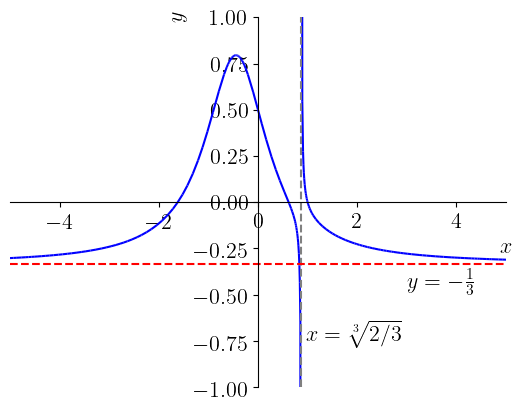
\includegraphics[width=0.7\textwidth]{./cap_lim/dados/fig_ex_ass_horizon/fig_ex_ass_horizon}
      \caption{Esboço do gráfico da função $\displaystyle f(x) = \frac{x^3 - 2x + 1}{2 - 3x^3}$.}
      \label{fig:ex_ass_horizon}
    \end{figure}

  Também, temos
  \begin{align}
    & \lim_{x\to -\infty} \frac{x^3 - 2x + 1}{2 - 3x^3} = \lim_{x\to\infty} \frac{x^3}{-3x^3} \\
    & \text{}\quad = -\frac{1}{3}.
  \end{align}
  O que reforça que $y = -1/3$ é uma assíntota horizontal desta função.
\end{ex}

\begin{ex}\normalfont{(Função exponencial natural)}\label{ex:lim_exp_x-inf}
  \begin{equation}
    \lim_{x\to -\infty} e^x = 0,
  \end{equation}
  donde temos que $y=0$ é uma assíntota horizontal da função exponencial natural. Veja a Figura \ref{fig:lim_ex_xinf_exp}.

  \begin{figure}[H]
    \centering
    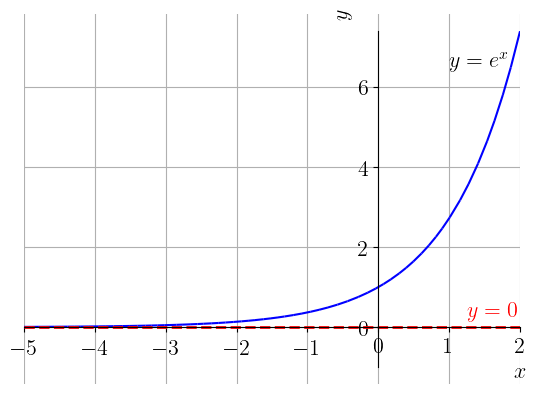
\includegraphics[width=0.7\textwidth]{./cap_lim/dados/fig_ex_xinf_exp/fig_ex_xinf_exp}
    \caption{Esboço do gráfico de $f(x)=e^x$.}
    \label{fig:lim_ex_xinf_exp}
  \end{figure}
\end{ex}

\begin{ex}\normalfont{(Função logística)}
  Na ecologia, a função logística \footnote{Consulte mais em \href{https://pt.wikipedia.org/wiki/Fun\%C3\%A7\%C3\%A3o_log\%C3\%ADstica}{Wikipédia}.}
    \begin{equation}
      P(t) = \frac{K}{1 + \left(\frac{K-P_0}{P_0}e^{-rt}\right)}
    \end{equation}
    é um modelo de crescimento populacional de espécies, sendo $P(t)$ o número de indivíduos da população no tempo $t$. O parâmetro $P_0$ é o número de indíviduos na população no tempo inicial $t=0$, $r>0$ é a proporção de novos indivíduos na população devido a reprodução e $K$ é o limite de saturação do crescimento populacional (devido aos recursos escassos como alimentos, território e tratamento a doenças). Observamos que
    \begin{equation}
      \lim_{t\to\infty} P(t) = \lim_{t\to\infty} \frac{K}{1 + \left(\frac{K-P_0}{P_0}\cancelto{0}{e^{-rt}}\right)} = K
    \end{equation}
    Ou seja, $P(t) = K$ é uma assíntota horizontal ao gráfico de $P = P(t)$ e é o limite de saturação do crecimento populacional. Na Figura \ref{fig:liminf_ex_funlogic}, temos o esboço do gráfico da função logística para $t\geq 0$.

    \begin{figure}[H]
      \centering
      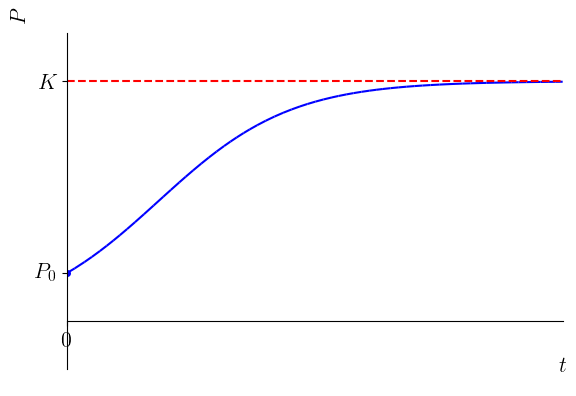
\includegraphics[width=0.7\textwidth]{./cap_lim/dados/fig_liminf_ex_funlogic/fig_liminf_ex_funlogic}
      \caption{Esboço do gráfico da função logistica.}
      \label{fig:liminf_ex_funlogic}
    \end{figure}
\end{ex}

\subsection{Limite no infinito de função periódica}

\begin{flushright}
  [Vídeo] | [Áudio] | \href{https://phkonzen.github.io/notas/contato.html}{[Contatar]}
\end{flushright}

Uma função $f$ é periódica quando existe um número $T$ tal que
\begin{equation}
  f(x) = f(x+T),
\end{equation}
para todo $x\in\mathbb{R}$ no domínio de $f$. As funções trigonométricas são exemplos de funções periódicas\footnote{Consulte mais nas \href{https://phkonzen.github.io/notas/PreCalculo/cap\_funcao\_sec\_funtri.html}{Notas de Aula - Pré-Cálculo - Funções Trigonométricas}}.

O limite no infinito de funções periódicas não existe\footnote{À exceção de funções constantes.}. De fato, se $f$ não é constante, então existem números $x_1\neq x_2$ tal que $y_1=f(x_1)\neq f(x_2)=y_2$. Como a função é periódica, $f(x_1+kT)=y_1$ e $f(x_2+kT) = y_2$ para todo número inteiro $k$. Desta forma, não existe número $L$ que possamos tomar $f(x)$ arbitrariamente próxima, para todos os valores de $x$ suficientemente grandes (ou pequenos).

\begin{ex}
  Não existe
  \begin{equation}
    \lim_{x\to \infty} \sen(x),
  \end{equation}
  pois os valores de $\sen x$ oscilam periodicamente no intervalo $[-1, 1]$. Veja a Figura \ref{fig:lim_senx_xinf}.

  \begin{figure}[H]
    \centering
    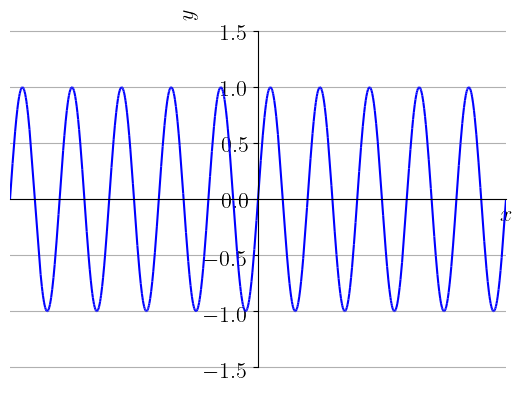
\includegraphics[width=0.7\textwidth]{./cap_lim/dados/fig_lim_senx_xinf/fig_lim_senx_xinf}
    \caption{Esboço do gráfico de $f(x)=\sen x$.}
    \label{fig:lim_senx_xinf}
  \end{figure}

  Com o {\python}+{\sympy}, temos

  \begin{lstlisting}
    >>> from sympy import *
    >>> x = Symbol("x")
    >>> limit(sin(x), x, oo)
    AccumBounds(-1, 1)
  \end{lstlisting}

  indicando que o limite não existe, pois $\sen x$ oscila indefinidamente no intervalo $[-1, 1]$.
\end{ex}


\subsection{Exercícios resolvidos}

\begin{exeresol}
  Calcule
  \begin{equation}
    \lim_{x\to \infty} \frac{1}{x-1}+1.
  \end{equation}
\end{exeresol}
\begin{resol}
  Utilizando a regra da soma para limites no infinito, temos
  \begin{align}
    & \lim_{x\to\infty} \frac{1}{x-1} + 1 = \lim_{x\to \infty} \frac{1}{x-1} + \lim_{x\to 1} 1 \\
    & \text{}\quad = \lim_{x\to \infty} \left(\frac{1}{x-1}\right)+1,
  \end{align}
  observando que $\lim_{x\to \infty}1/(x-1)$ existe. De fato, o gráfico de $g(x) = 1/(x-1)$ é uma translação de uma unidade à esquerda da função $f(x)=1/x$. Uma translação horizontal finita não altera o comportamento da função para $x\to \infty$. Portanto, como $f(x)=1/x\to\infty$ quando $x\to\infty$, temos que $g(x)=f(x-1)=1/(x-1)\to\infty$ quando $x\to\infty$, i.e.
  \begin{equation}
    \lim_{x\to\infty}\frac{1}{x-1} = 0.
  \end{equation}
  Portanto, concluímos que
  \begin{equation}
    \lim_{x\to \infty} \frac{1}{x-1} + 1 = 1. 
  \end{equation}

  \ifispython
  Com o {\python}+{\sympy}, podemos computar este limite com o seguinte comando:
  \begin{lstlisting}
    >>> from sympy import *
    >>> x = Symbol("x")
    >>> limit(1/(x-1)+1, x, oo)
    1
  \end{lstlisting}
  \fi
\end{resol}

\begin{exeresol}
  Determine a(s) assíntota(s) horizontal(ais) do gráfico da função
  \begin{equation}
    f(x) = \frac{3 - x + 4x^4 - 10x^3}{x^2 + 2x^4 -x}.
  \end{equation}
\end{exeresol}
\begin{resol}
  Uma reta $y = L$ é assíntota horizontal do gráfico de $f$, quando
  \begin{equation}
    \lim_{x\to\pm\infty} f(x) = L.
  \end{equation}
  Começamos com $x\to-\infty$, temos
  \begin{align}
    & \lim_{x\to-\infty} f(x) = \lim_{x\to-\infty} \frac{3 - x + 4x^4 - 10x^3}{x^2 + 2x^4 -x} \\
    & \text{}\quad = \lim_{x\to -\infty} \frac{4x^4}{2x^4} = 2.
  \end{align}
  Logo, $y=2$ é assíntota horizontal ao gráfico de $f(x)$.

  Agora, vamos ver a tendência da função para $x\to\infty$, temos
  \begin{align}
    & \lim_{x\to\infty} f(x) = \lim_{x\to\infty} \frac{3 - x + 4x^4 - 10x^3}{x^2 + 2x^4 -x} \\
    & \text{}\quad = \frac{4}{2} = 2.
  \end{align}
  Portanto, concluímos que $y=2$ é a única assíntota horizontal ao gráfico da função $f$.

  \ifispython
  Os seguintes comandos do {\python}+{\sympy} permitem plotar o esboço do gráfico da função $f$ (linha azul) e sua assíntota horizontal (linha vermelha):
  \begin{lstlisting}
    >>> from sympy import *
    >>> x = Symbol("x")
    >>> f = lambda x: (3-x+4*x**4-10*x**3)/(x**2+2*x**4-x)
    >>> L = limit(f(x), x, oo)
    >>> p = plot(f(x), (x, -15, 15), ylim = [-4, 6],\
        line_color = "blue", show = False)
    >>> q = plot(L, (x, -15, 15), line_color = "red", show = False)
    >>> p.extend(q)
    >>> p.show()
  \end{lstlisting}
  \fi
\end{resol}

\begin{exeresol}
  Calcule
  \begin{equation}
    \lim_{x\to \infty} e^{-x}.
  \end{equation}
\end{exeresol}
\begin{resol}
  Observamos que o gráfico de $f(x)=e^{-x}$ é uma reflexão em torno do eixo $y$ do gráfico da função $g(x)=e^x$. No Exemplo \ref{ex:lim_exp_x-inf}, vimos que
  \begin{equation}
    \lim_{x\to -\infty} g(x) = \lim_{x\to -\infty} e^{x} = 0,
  \end{equation}
  logo
  \begin{align}
    & \lim_{x\to \infty} e^{-x} = \lim_{x\to \infty} g(-x) \\
    & \text{}\quad = \lim_{x\to -\infty} g(x) = 0.
  \end{align}
  Veja o esboço do gráfico de $f(x)=e^{-x}$ na Figura \ref{fig:exeresol_lim_exp_xinf}.

  \begin{figure}[H]
    \centering
    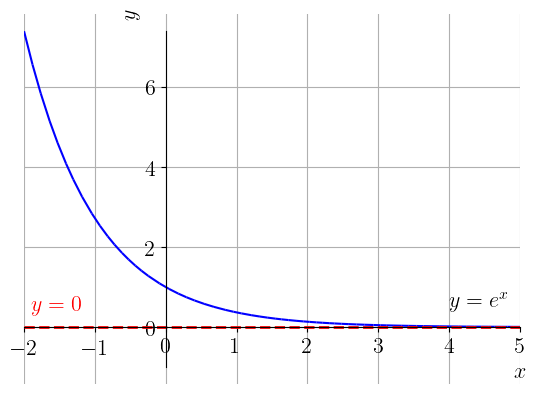
\includegraphics[width=0.7\textwidth]{./cap_lim/dados/fig_exeresol_lim_exp_xinf/fig_exeresol_lim_exp_xinf}
    \caption{Esboço do gráfico de $f(x)=e^{-x}$.}
    \label{fig:exeresol_lim_exp_xinf}
  \end{figure}  

  \ifispython
  Com o {\python}+{\sympy}, podemos computar este limite com o seguinte comando:
  \begin{lstlisting}
    >>> from sympy import *
    >>> x = Symbol("x")
    >>> limit(exp(-x), x, oo)
    0
  \end{lstlisting}
  \fi
\end{resol}

\subsection{Exercícios}

\begin{exer}
  Calcule
  \begin{enumerate}[a)]
  \item $\displaystyle\lim_{x\to\infty} \frac{10}{x}$
  \item $\displaystyle\lim_{x\to -\infty} -10x^{-1}$
  \item $\displaystyle\lim_{x\to -\infty} -\frac{10}{x^2}$
  \item $\displaystyle\lim_{x\to\infty} \frac{1}{x-\sqrt{2}}$
  \item $\displaystyle\lim_{x\to -\infty} 2 - (x+1)^{-1}$
\end{enumerate}
\end{exer}
\begin{resp}
  a) $0$; b) $0$; c) $0$; d) $0$; e) $2$; 
\end{resp}

\begin{exer}
  Calcule
  \begin{enumerate}[a)]
  \item $\displaystyle\lim_{x\to\infty} x^{-\frac{1}{2}}$ 
  \item $\displaystyle\lim_{x\to -\infty} \frac{1}{\sqrt{(x+1)^3}}$ 
  \item $\displaystyle\lim_{x\to \infty} x^{-s},\quad s>0$ 
  \end{enumerate}
\end{exer}
\begin{resp}
  a) $0$; b) $0$; c) $0$
\end{resp}

\begin{exer}
  Calcule
  \begin{enumerate}[a)]
  \item $\displaystyle \lim_{x\to -\infty} 2^{x}$
  \item $\displaystyle \lim_{x\to \infty} \left(\frac{1}{2}\right)^x+1$
  \item $\displaystyle \lim_{x\to -\infty} 2\cdot 3^x + \sqrt{2}$
  \end{enumerate}
\end{exer}
\begin{resp}
  a)~$0$; b)~$1$; c)~$\sqrt{2}$;
\end{resp}

\begin{exer}
  Calcule
  \begin{enumerate}[a)]
  \item $\displaystyle \lim_{x\to -\infty} e^x+1$
  \item $\displaystyle \lim_{x\to \infty} 3 + e^{-x}$
  \item $\displaystyle \lim_{x\to \infty} 2e^{-x}-1$
  \item $\displaystyle \lim_{x\to -\infty} e-e^{x}$
  \end{enumerate}
\end{exer}
\begin{resp}
  a)~$1$; b)~$3$; c)~$-1$; d)~$e$
\end{resp}

\begin{exer}
  Calcule
  \begin{enumerate}[a)]
  \item $\displaystyle\lim_{x\to \infty} \frac{\sqrt{1+x^2}}{2x}$
  \item $\displaystyle\lim_{x\to -\infty} \frac{\sqrt{1+x^2}}{2x}$
\end{enumerate}
\end{exer}
\begin{resp}
  a) $\frac{1}{2}$; b) $-\frac{1}{2}$
\end{resp}

\begin{exer}
  Calcule
  \begin{equation}
    \lim_{x\to -\infty} \cos x.
  \end{equation}
\end{exer}
\begin{resp}
  não existe.
\end{resp}

\begin{exer}
  Calcule:
  \begin{enumerate}[a)]
  \item $\displaystyle\lim_{x\to \infty} \sqrt{1+e^{-x}}$.
  \item $\displaystyle\lim_{x\to -\infty} \frac{1-2x}{x+3} -e^{x} - 1$.
  \end{enumerate}
\end{exer}
\begin{resp}
  a)~$1$; b)~$-3$
\end{resp}

\begin{exer}\label{exer:lim_xinf_racio}
  Dados dois polinômios $p(x) = a_nx^n+a_{n-1}x^{n-1}+\cdots + a_0$ e $q(x) = b_mx^m+b_{m-1}x^{m-1}+\cdots + b_0$, mostre que
  \begin{equation}
    \lim_{x\to \pm\infty} \frac{p(x)}{q(x)} = \lim_{x\to\pm\infty}\frac{a_nx^n}{b_mx^m}.
  \end{equation}
\end{exer}
\begin{resp}
  Dica: use as regras para o cálculo de limites.
\end{resp}

\ifisbook
\subsubsection{Respostas}
\shipoutAnswer
\fi

\section{Limites infinitos}\label{cap_lim_sec_lim_inf}
\badgeYouTube{KsWI1qgzr88}

O limite de uma função nem sempre existe. Entretanto, em muitos destes casos, podemos concluir mais sobre a tendência da função. Por exemplo, dizemos que o limite de uma dada função $f(x)$ é infinito quando $x$ tende a um número $x_0$, se $f(x)$ é arbitrariamente grande para todos os valores de $x$ suficientemente próximos de $x_0$, mas $x\neq x_0$. Neste caso, escrevemos
\begin{equation}
  \lim_{x\to x_0} f(x) = \infty.
\end{equation}
A Figura \ref{fig:liminf}, é uma ilustração de $f(x)\to\infty$ quando $x\to x_0$.

\begin{figure}[H]
  \centering
  \includegraphics[width=0.7\textwidth]{./cap_lim/dados/fig_liminf/fig}
  \caption{Ilustração de $f(x)\to\infty$ quando $x\to x_0$.}
  \label{fig:liminf}
\end{figure}


\begin{ex}
  Vejamos o caso de
  \begin{equation}
    \lim_{x\to 0} \frac{1}{x^2}.
  \end{equation}
  Ao tomarmos $x$ próximo de $x_0=0$, obtemos os seguintes valores de $f(x)$:
  \begin{center}
    \begin{tabular}[H]{l|ccc|c|ccc}
      $x$ & $-10^{-1}$ & $-10^{-2}$ & $-10^{-3}$ & $\rightarrow 0 \leftarrow$ & $10^{-3}$ & $10^{-2}$ & $10^{-1}$ \\\hline
      $f(x)$ & $10^{2}$ & $10^{4}$ & $10^{6}$ & $\rightarrow \infty \leftarrow$ & $10^{6}$ & $10^{4}$ & $10^{2}$
    \end{tabular}
  \end{center}
  Veja o esboço do gráfico de $f(x)$ na Figura \ref{fig:ex_liminf_1x2}.

\begin{figure}[H]
  \centering
  \includegraphics[width=0.7\textwidth]{./cap_lim/dados/fig_ex_liminf_1x2/fig}
  \caption{Esboço do gráfico de $f(x)=1/x^2$.}
  \label{fig:ex_liminf_1x2}
\end{figure}  

  Podemos concluir que os valores de $f(x)$ podem ser tomados arbitrariamente grandes ao escolhermos qualquer $x$ suficientemente próximo de $0$, com $x\neq 0$. I.e.,
  \begin{equation}
    \lim_{x\to 0}\frac{1}{x^2} = \infty.
  \end{equation}

  \ifispython
  Com o {\python}+{\sympy}, podemos computar este limite com o seguinte comando:
  \begin{lstlisting}
    >>> from sympy import *
    >>> x = Symbol("x")
    >>> limit(1/x**2, x, 0)
    oo
  \end{lstlisting}
  Atenção! Na verdade, este comando computa o limite lateral à direita. Na sequência, discutimos sobre limites laterais infinitos.
  \fi
\end{ex}

Definimos os limites laterais infinitos
\begin{equation}
  \lim_{x\to x_0^-} f(x) = \infty
\end{equation}
e
\begin{equation}
  \lim_{x\to x_0^+} f(x) = \infty.
\end{equation}
No primeiro caso, os valores de $f(x)$ são arbitrariamente grandes conforme os valores de $x\to x_0$ e $x<x_0$. No segundo caso, os valores de $f(x)$ são arbitrariamente grandes conforme os valores de $x\to x_0$ e $x>x_0$.

\begin{ex}
  \begin{equation}
    \lim_{x\to 1^+} \frac{1}{x-1} = \infty.
  \end{equation}
  De fato, conforme tomamos valores de $x$ próximos de $1$, com $x>1$, os valores de $f(x) = 1/(x-1)$ tornam-se cada vez maiores. Veja o esboço do gráfico de $f(x)$ na Figura \ref{fig:ex_liminf_1x}.

\begin{figure}[H]
  \centering
  \includegraphics[width=0.7\textwidth]{./cap_lim/dados/fig_ex_liminf_1x/fig}
  \caption{Esboço do gráfico de $f(x)=1/(x-1)$.}
  \label{fig:ex_liminf_1x}
\end{figure}  

\ifispython
  Com o {\python}+{\sympy}, podemos computar este limite com o seguinte comando:
  \begin{lstlisting}
    >>> from sympy import *
    >>> x = Symbol("x")
    >>> limit(1/(x-1), x, 1, '+')
    oo
  \end{lstlisting}
\fi
\end{ex}


Analogamente a definição de limite infinito, dizemos que o limite de uma dada função $f(x)$ é menos infinito quando $x$ tende a $x_0$, quando $f(x)$ torna-se arbitrariamente pequeno para valores de $x$ suficientemente próximos de $x_0$, com $x\neq x_0$. Neste caso, escrevemos
\begin{equation}
  \lim_{x\to x_0} f(x) = -\infty.
\end{equation}
De forma similar, definimos os limites laterais $f(x)\to -\infty$ quando $x\to x_0^{\pm}$.

\begin{ex}
  Observe que
  \begin{equation}
    \nexists \lim_{x\to 0} \frac{1}{x}
  \end{equation}
  e que não podemos concluir que este limite é $\infty$ ou $-\infty$. Isto ocorre, pois
  \begin{equation}
    \lim_{x\to 0^-} \frac{1}{x} = -\infty
  \end{equation}
  e
  \begin{equation}
    \lim_{x\to 0^+} \frac{1}{x} = +\infty.
  \end{equation}
\end{ex}

\begin{ex}
  \begin{equation}
    \lim_{x\to -1} \frac{-1}{(x+1)^2} = -\infty.
  \end{equation}
  De fato, podemos inferir este limite a partir do gráfico da função $f(x) = 1/(x+1)^2$. Este é uma translação de uma unidade à esquerda do gráfico de $y = 1/x^2$, seguida de uma reflexão em torno de eixo $x$. Veja a Figura \ref{fig:ex_liminf-1x2}.

  \begin{figure}[H]
    \centering
    \includegraphics[width=0.7\textwidth]{./cap_lim/dados/fig_ex_liminf-1x2/fig}
    \caption{Esboço do gráfico de $f(x)=-1/(x+1)^2$.}
    \label{fig:ex_liminf-1x2}
  \end{figure}

  Com o {\python}+{\sympy}, podemos computar este limite com o seguinte comando:
  
  \begin{lstlisting}
    >>> from sympy import *
    >>> x = Symbol("x")
    >>> limit(-1/(x+1)**2, x, -1)
    -oo
  \end{lstlisting}
  
  Novamente, observamos que este comando computa apenas o limite lateral à direita.

\end{ex}

\subsection{Assíntotas verticais}
\badgeYouTube{5OFKyRGG9lU}
% \begin{flushright}
%   \href{https://youtu.be/5OFKyRGG9lU}{[YouTube]} | \href{https://archive.org/details/video_20220727}{[Vídeo]} | [Áudio] | \href{https://phkonzen.github.io/notas/contato.html}{[Contatar]}
% \end{flushright}

Uma reta $x=x_0$ é uma {\bf assíntota vertical} do gráfico de uma função $y = f(x)$ se
\begin{equation}
  \lim_{x\to x_0^-} f(x) = \pm\infty
\end{equation}
ou
\begin{equation}
  \lim_{x\to x_0^+} f(x) = \pm\infty.
\end{equation}

\begin{ex}
  O gráfico da função $f(x)=-1/|x|$ tem uma assíntota vertical em $x=0$, pois
  \begin{equation}
    \lim_{x\to 0} \frac{-1}{|x|} = -\infty.
  \end{equation}
  Veja o esboço de seu gráfico na Figura \ref{fig:ex_lim_assvert_1}.

  \begin{figure}[H]
    \centering
    \includegraphics[width=0.7\textwidth]{./cap_lim/dados/fig_ex_lim_assvert_1/fig}
    \caption{Esboço do gráfico de $f(x)=-1/|x|$.}
    \label{fig:ex_lim_assvert_1}
  \end{figure}  
\end{ex}

\begin{ex}
  A função $\displaystyle f(x) = \frac{x^3 + 2x^2 - 4x - 8}{x^2 - 1}$ não está definida para valores de $x$ tais que seu denominador se anule, i.e.
    \begin{align}
      & x^2 - 1 = 0 \\
      & x_0=-1\quad\text{ou}\quad x_1=1
    \end{align}
    Nestes pontos o gráfico de $f$ pode ter assíntotas verticais. De fato, temos
    \begin{align}
      & \lim_{x\to -1^+} \frac{\cancelto{-3}{x^3 + 2x^2 - 4x - 8}}{\cancelto{0^-}{x^2-1}} =  +\infty,\\
      & \lim_{x\to -1^-} \frac{\cancelto{-3}{x^3 + 2x^2 - 4x - 8}}{\cancelto{0^+}{x^2-1}} =  -\infty,
    \end{align}
    e, também, temos
    \begin{align}
      & \lim_{x\to 1^+} \frac{\cancelto{-9}{x^3 + 2x^2 - 4x - 8}}{\cancelto{0^+}{x^2-1}} = -\infty,\\      
      & \lim_{x\to 1^-} \frac{\cancelto{-9}{x^3 + 2x^2 - 4x - 8}}{\cancelto{0^-}{x^2-1}} = +\infty.
    \end{align}
    Com isso, temos que as retas $x=-1$ e $x=1$ são assíntotas verticais ao gráfico da função $f$. Veja a Figura \ref{fig:ex_lim_assvert_racio} para o esboço do gráfico desta função.

    \begin{figure}[H]
      \centering
      \includegraphics[width=0.7\textwidth]{./cap_lim/dados/fig_ex_lim_assvert_racio/fig}
      \caption{Função $\displaystyle f(x) = \frac{x^3 + 2x^2 - 4x - 8}{x^2 - 1}$.}
      \label{fig:ex_lim_assvert_racio}
    \end{figure}
\end{ex}

\begin{ex}\normalfont{(Função logarítmica)}
  A função logarítmica natural $y = \ln x$ é tal que
  \begin{equation}
    \lim_{x\to 0^+} \ln x = -\infty
  \end{equation}
  i.e., $x=0$ é uma assíntota vertical ao gráfico de $\ln x$. Isto decorre do fato de $y = \ln x$ ser a função inversa de $y = e^x$ e, esta, ter uma assíntota horizontal $y=0$\footnote{Veja o Exemplo \ref{ex:lim_exp_x-inf}.}. A Figura \ref{fig:ex_lim_assvert_lnx} é um esboço do gráfico da função  $\ln x$.

    \begin{figure}[H]
      \centering
      \includegraphics[width=0.7\textwidth]{./cap_lim/dados/fig_ex_lim_assvert_lnx/fig}
      \caption{Esboço do gráfico da função logaritmo natural.}
      \label{fig:ex_lim_assvert_lnx}
    \end{figure}  
\end{ex}

\begin{ex}
  As funções trigonométricas $y = \tg x$ e $y = \sec x$ têm assíntotas verticais $x = (2k+1)\frac{\pi}{2}$ para $k$ inteiro. Já, as funções trigonométricas $y = \cotg x$ e $y = \cossec x$ têm assíntotas verticais $x = k\pi$ para $k$ inteiro. Consulte mais em \href{https://notaspedrok.com.br/notas/PreCalculo/cap_funcao_sec_funtri.html}{Funções Trigonométricas} nas \href{https://notaspedrok.com.br/notas/PreCalculo/main.html}{Notas de Aula de Pré-Cálculo}.
\end{ex}

\subsection{Assíntotas oblíquas}

\begin{flushright}
  [Vídeo] | [Áudio] | \href{https://phkonzen.github.io/notas/contato.html}{[Contatar]}
\end{flushright}

Além de assíntotas horizontais e verticais, gráficos de funções podem ter assintota oblíquas. Isto ocorre, particularmente, para funções racionais cujo grau do numerador é maior que o do denominador.

\begin{figure}[H]
  \centering
  \includegraphics[width=0.7\textwidth]{./cap_lim/dados/fig_ex_ass_obl/fig}
  \caption{Esboço do gráfico da função $\displaystyle f(x) = \frac{x^2-1}{5x-4}$.}
  \label{fig:ex_ass_obl}
\end{figure}


\begin{ex}
  Consideremos a função racional
  \begin{equation}
    f(x) = \frac{x^2-1}{5x-4}.
  \end{equation}
  Para buscarmos determinar a assíntota oblíqua desta função, dividimos o numerador pelo denominador, de forma a obtermos
  \begin{equation}
    f(x) = \underbrace{\left(\frac{x}{5}+\frac{4}{25}\right)}_{\text{quociente}} + \underbrace{\frac{-\frac{9}{25}}{5x-4}}_{\text{resto}}.
  \end{equation}
  Observamos, agora, que o resto tende a zero quando $x\to\pm\infty$, i.e. $\displaystyle f(x)\to \frac{x}{5}+\frac{4}{25}$ quando $x\to\pm\infty$. Com isso, concluímos que $\displaystyle y = \frac{x}{5}+\frac{4}{25}$ é uma assíntota oblíqua ao gráfico de $f(x)$. Veja a Figura \ref{fig:ex_ass_obl}.
\end{ex}

\begin{obs}
  Analogamente à assintotas oblíquas, podemos ter outros tipos de assíntotas determinadas por funções de diversos tipos, por exemplo, assíntotas quadráticas.
\end{obs}

\subsection{Limites infinitos no infinito}

\begin{flushright}
  [Vídeo] | [Áudio] | \href{https://phkonzen.github.io/notas/contato.html}{[Contatar]}
\end{flushright}

Escrevemos
\begin{equation}
  \lim_{x\to\infty} f(x)=\infty,
\end{equation}
quando os valores da função $f$ são arbitrariamente grandes para todos os valores de $x$ suficientemente grandes. De forma análoga, definimos
\begin{equation}
  \lim_{x\to -\infty} f(x)=\infty,
\end{equation}
\begin{equation}
  \lim_{x\to \infty} f(x)=-\infty
\end{equation}
e
\begin{equation}
  \lim_{x\to -\infty} f(x)=-\infty.
\end{equation}

\begin{ex}
  Vejamos os seguintes casos:
  \begin{enumerate}[a)]
  \item $\displaystyle\lim_{x\to\infty} x^2 = \infty$
  \item $\displaystyle\lim_{x\to -\infty} x^2 = \infty$
  \item $\displaystyle\lim_{x\to -\infty} x^3 = -\infty$
  \item $\displaystyle\lim_{x\to \infty} e^x = \infty$
  \item $\displaystyle\lim_{x\to \infty} \ln x = \infty$
  \item $\displaystyle\lim_{x\to -\infty} e^{-x} = \infty$
  \end{enumerate}
\end{ex}

\begin{ex}\label{ex:liminf_poli}
  \begin{align}
    & \lim_{x\to \infty} x^3 - 10x^2 + 300 = \lim_{x\to \infty} \frac{x^3 - 10x^2 + 300}{1}\cdot\frac{\frac{1}{x^3}}{\frac{1}{x^3}} \\
    & \text{}\quad = \lim_{x\to \infty} \frac{1 - \cancelto{0^+}{\frac{10}{x}} + \cancelto{0^+}{\frac{300}{x^3}}}{\cancelto{0^+}{\frac{1}{x^3}}} = \infty.                                   
  \end{align}
\end{ex}

\begin{prop}
  Dado um polinômio $p(x) = a_nx^n + a_{n-1}x^{n-1} + \cdots + a_0$, temos
  \begin{equation}
    \lim_{x\to \pm\infty} p(x) = \lim_{x\to\pm} a_nx^n.
  \end{equation}
\end{prop}

\begin{ex}
  Retornando ao exemplo anterior (Exemplo \ref{ex:liminf_poli}, temos
  \begin{align}
    & \lim_{x\to \infty} x^3 - 10x^2 + 300 = \lim_{x\to \infty} x^3 \\
    & \text{}\quad = \infty.
  \end{align}
\end{ex}

\subsection{Exercícios resolvidos}

% \begin{flushright}
%   [Vídeo] | [Áudio] | \href{https://phkonzen.github.io/notas/contato.html}{[Contatar]}
% \end{flushright}

\begin{exeresol}
  Calcule
  \begin{equation}
    \lim_{x\to 1^-} \frac{x-2}{1-x}. 
  \end{equation}
\end{exeresol}
\begin{resol}
  Temos
  \begin{equation}
    \lim_{x\to 1^-} \frac{\cancelto{-1}{x-2}}{\cancelto{0^+}{1-x}} = -\infty.
  \end{equation}

  Outra forma de calcular este limite é observar que $y = 1-x\to 0^+$ quando $x\to 1^-$. Assim, fazendo a mudança de variável $y = x-1$, temos
  \begin{align}
    & \lim_{x\to 1^-} \frac{x-2}{1-x} = \lim_{y\to 0^+} \frac{y+1-2}{y} \\
    & \text{}\quad = \lim_{y\to 0^+} \frac{y-1}{y} \\
    & \text{}\quad = -\infty.
  \end{align}

  \ifispython
  Podemos usar o seguinte comando{\python}+{\sympy} para computar este limite:
  \begin{lstlisting}
    >>> from sympy import *
    >>> x = Symbol("x")
    >>> limit((x-2)/(1-x), x, 1, '-')
    -oo
  \end{lstlisting}
  \fi
\end{resol}

\begin{exeresol}
  Calcule
  \begin{equation}
    \lim_{x\to 1} \ln |x-1|.
  \end{equation}
\end{exeresol}
\begin{resol}
  Começamos observando que
  \begin{equation}
    \ln |x-1| = \left\{
      \begin{array}{ll}
        \ln(1-x) &, x < 1,\\
        \ln(x-1) &, x > 1.
      \end{array}
    \right.
  \end{equation}
  Então, calculando o limite lateral à esquerda, temos
  \begin{align}
    & \lim_{x\to 1^-} \ln |x-1| = \lim_{x\to 1^-} \ln(1-x) \\
    & \text{}\quad = \lim_{y\to 0^+} \ln y = -\infty\footnote{Observe que $1-x\to 0^+$ quando $x\to 1^-$.}.
  \end{align}
  Por outro lado, temos
  \begin{align}
    & \lim_{x\to 1^+} \ln |x-1| = \lim_{x\to 1^+} \ln(x-1) \\
    & \text{}\quad = \lim_{y\to 0^+} \ln y = -\infty\footnote{Observe que $x-1\to 0^+$ quando $x\to 1^+$.}.
  \end{align}
  Portanto, concluímos que
  \begin{equation}
    \lim_{x\to 1} \ln |x-1| = -\infty.
  \end{equation}

  \ifispython
  Podemos usar os seguintes comandos {\python}+{\sympy} para computar os limites laterais:
  \begin{lstlisting}
    >>> from sympy import *
    >>> x = Symbol("x")
    >>> limit(log(abs(x-1)), x, 1, '-')
    -oo
    >>> limit(log(abs(x-1)), x, 1, '+')
    -oo
  \end{lstlisting}
  \fi
\end{resol}

\begin{exeresol}
  Calcule
  \begin{equation}
    \lim_{x\to \infty} \frac{x^3+2x^2-4x-8}{x^2-1}.
  \end{equation}
\end{exeresol}
\begin{resol}
  Tratando-se de uma função racional, temos\footnote{Veja a Observação \ref{prop:lim_xinf_racio}. Veja, também, o gráfico desta função na Figura \ref{fig:ex_lim_assvert_racio}.}
  \begin{align}
    & \lim_{x\to \infty} \frac{x^3+2x^2-4x-8}{x^2-1} = \lim_{x\to\infty} \frac{x^3}{x^2} \\
    & \text{}\quad = \lim_{x\to \infty} x \\
    & \text{}\quad = \infty.    
  \end{align}
\end{resol}

\begin{exeresol}
  Calcule
  \begin{equation}
    \lim_{x\to \infty} e^{1-x^2}.
  \end{equation}
\end{exeresol}
\begin{resol}
  Observamos que $1-x^2\to -\infty$ quando $x\to \infty$. Desta forma, fazendo a mudança de variáveis $y = 1 - x^2$, temos
  \begin{equation}
    \lim_{x\to\infty} e^{1-x^2} = \lim_{y\to -\infty} e^y = 0.
  \end{equation}
\end{resol}

\begin{exeresol}
  Calcule
  \begin{equation}
    \lim_{x\to\infty} \frac{\sqrt{1+x^2}}{2x}.
  \end{equation}
\end{exeresol}
\begin{resol}
  Podemos verificar que trata-se de uma indeterminação do tipo $\infty/\infty$. Neste caso, podemos calcular o limite pela multiplicação (em cima e em baixo) pelo inverso do fator dominante no radical, i.e. $1/\sqrt{x^2}$. Ou seja, calculamos
  \begin{align}
    & \lim_{x\to\infty} \frac{\sqrt{1+x^2}}{2x} = \lim_{x\to\infty} \frac{\sqrt{1+x^2}}{x}\cdot \frac{\frac{1}{\sqrt{x^2}}}{\frac{1}{\sqrt{x^2}}} \\
    & \text{}\quad = \lim_{x\to\infty} \frac{\sqrt{\frac{1}{x^2}+\frac{x^2}{x^2}}}{2\frac{x}{\sqrt{x^2}}}.
  \end{align}
  Lembramos que $\sqrt{x^2}=|x|$. Como $x\to\infty$, temos $\sqrt{x^2} = |x|=x$. Logo,
  \begin{align}
    & \lim_{x\to\infty} \frac{\sqrt{\frac{1}{x^2}+\frac{x^2}{x^2}}}{2\frac{x}{\sqrt{x^2}}} = \lim_{x\to\infty} \frac{\sqrt{\frac{1}{x^2}+\frac{x^2}{x^2}}}{2\frac{x}{|x|}} \\
    & \text{}\quad = \lim_{x\to\infty} \frac{\sqrt{\frac{1}{x^2}+1}}{2\frac{x}{x}} \\
    & \text{}\quad = \lim_{x\to\infty} \frac{1}{2}\sqrt{\frac{1}{x^2}+1} \\
    & \text{}\quad = \frac{1}{2}\sqrt{\lim_{x\to\infty} \frac{1}{x^2}+1} \\
    & \text{}\quad = \frac{1}{2}.
  \end{align}
\end{resol}


\subsection{Exercícios}

\begin{exer}
  Calcule
  \begin{enumerate}[a)]
  \item $\displaystyle\lim_{x\to 0^+}x^{-1}$
  \item $\displaystyle\lim_{x\to 0^-}-x^{-3}$
  \item $\displaystyle\lim_{x\to 0^+}x^{-5}$
  \item $\displaystyle\lim_{x\to 0^\pm}x^{-n},\quad n>0 ~\text{ímpar}$
  \end{enumerate}
\end{exer}
\begin{resp}
  a) $\infty$; b) $\infty$; c) $\infty$; d) $\pm\infty$
\end{resp}

\begin{exer}
  Calcule
  \begin{enumerate}[a)]
  \item $\displaystyle\lim_{x\to 0^+}x^{-2}$
  \item $\displaystyle\lim_{x\to 0^-}x^{-4}$
  \item $\displaystyle\lim_{x\to 0^+}-x^{-6}$
  \item $\displaystyle\lim_{x\to 0^\pm}x^{-n},\quad n>0 ~\text{ímpar}$
  \end{enumerate}
\end{exer}
\begin{resp}
  a) $\infty$; b) $\infty$; c) $-\infty$; d) $\infty$
\end{resp}

\begin{exer}
  Calcule
  \begin{enumerate}[a)]
  \item $\displaystyle\lim_{x\to 1^+}\frac{1}{x-1}$
  \item $\displaystyle\lim_{x\to 1^-}\frac{-2}{x-1}$
  \item $\displaystyle\lim_{x\to -1^-}\frac{-2}{1+x}$
  \item $\displaystyle\lim_{x\to -1}\frac{-2}{(x+1)^2}$
  \item $\displaystyle\lim_{x\to -1} \frac{x^2 - 3x + 2}{x^2 + 2x + 1}$
  \end{enumerate}
\end{exer}
\begin{resp}
  a) $\infty$; b) $\infty$; c) $-\infty$; d) $-\infty$; e) $\infty$
\end{resp}

\begin{exer}
  Determine as assíntotas verticais ao gráfico da função
  \begin{equation}
    f(x) = \frac{8}{x^2-4}.
  \end{equation}
\end{exer}
\begin{resp}
  $x=2$; $x=-2$
\end{resp}

\begin{exer}
  Determine as assíntotas verticais ao gráfico da função
  \begin{equation}
    f(x) = \frac{x+1}{x^2-1}.
  \end{equation}
\end{exer}
\begin{resp}
  $x=1$
\end{resp}

\begin{exer}
  Calcule
  \begin{equation}
    \lim_{x\to -\infty} e^{x^2-1}.
  \end{equation}
\end{exer}
\begin{resp}
  $\infty$
\end{resp}

\begin{exer}
  Calcule
  \begin{equation}
    \lim_{x\to -\infty} x^3 + 10x^2 - 300.
  \end{equation}
\end{exer}
\begin{resp}
  $-\infty$
\end{resp}

\begin{exer}
  Mostre que $y = x^2$ é assíntota ao gráfico de
  \begin{equation}
    f(x) = \frac{x^3+1}{x}.
  \end{equation}
\end{exer}
\begin{resp}
  Dica: Observe que $f(x) = x^2 + \frac{1}{x}$ e analise o limite de $f(x)$ quando $x\to\pm\infty$.
\end{resp}

\begin{exer}(Aplicação)
  Na física química, a \href{https://pt.wikipedia.org/wiki/Equa\%C3\%A7\%C3\%A3o\_de\_Arrhenius}{Equação de Arrhenius}\footnote{Svante August Arrhenius, 1859-1927, químico sueco. Fonte: \href{https://pt.wikipedia.org/wiki/Svante\_Arrhenius}{Wikipédia}.} fornece a taxa de reação $k$ (entre espécies químicas) em função da temperatura $T$ [K]
  \begin{equation}
    k = Ae^{-\frac{E_a}{RT}}, 
  \end{equation}
  onde $A>0$ é o fator constante pré-exponencial, $E_a>0$ é a energia de ativação e $R>0$ é a constante universal dos gases. Para temperatura constante, a equação acima define a função $k = k(E_a)$. Qual é a tendência da taxa de reação $k$ quando $T\to 0^+$. 
\end{exer}
\begin{resp}
  $k\to 0$ quando $T\to 0^+$
\end{resp}

\begin{exer}(Aplicação.)
  A função logística tem aplicações em várias áreas do conhecimento como, por exemplo, na \href{https://pt.wikipedia.org/wiki/Intelig\%C3\%AAncia\_artificial}{inteligência artificial} e na modelagem de crescimento populacional\footnote{Consulte mais em \href{https://pt.wikipedia.org/wiki/Fun\%C3\%A7\%C3\%A3o\_log\%C3\%ADstica}{Wikipédia: Função Logística}.}. Ela tem a forma
  \begin{equation}
    \varphi(x) = \frac{1}{1 + e^{-x}}
  \end{equation}
  Encontre a(s) assíntota(s) horizontal(ais) dessa função logística.
\end{exer}
\begin{resp}
  $y=0$ e $y=1$
\end{resp}

\begin{exer}(Aplicação.)
  O fenômeno de desintegração espontânea do núcleo de um átomo com a emissão de algumas radiações é chamado de radioatividade\footnote{Fonte: \href{https://pt.wikipedia.org/wiki/Radioatividade}{Wikipédia}.}. A lei fundamental do decaimento radiativo estabelece que a taxa de decaimento é proporcional ao número de átomos que ainda não decaíram. Isto nos fornece a equação da lei básica da radioatividade
  \begin{equation}
    N = N_0e^{-\lambda t}
  \end{equation}
  onde, $N = N(t)$ é o número de átomos no tempo $t$, $N_0\geq 0$ é o número de átomos presentes no tempo inicial $t=0$ e $\lambda>0$ é a constante de decaimento. Qual a tendência de $N$ quando $t\to \infty$.
\end{exer}
\begin{resp}
  $N(t)\to 0$ quando $t\to \infty$
\end{resp}

\ifisbook
\subsubsection{Respostas}
\shipoutAnswer
\fi


\section{Continuidade}\label{cap_lim_sec_cont}

\begin{flushright}
  [Vídeo] | [Áudio] | \href{https://phkonzen.github.io/notas/contato.html}{[Contatar]}
\end{flushright}

\subsection{Definição de função contínua}

\begin{flushright}
  [Vídeo] | [Áudio] | \href{https://phkonzen.github.io/notas/contato.html}{[Contatar]}
\end{flushright}

Dizemos que uma {\bf função} $f$ é {\bf contínua} em um ponto $x_0$, quando $f(x_0)$ está definida, existe o limite
\begin{equation}
  \lim_{x\to x_0} f(x)
\end{equation}
e
\begin{equation}
  \lim_{x\to x_0} f(x) = f(x_0).
\end{equation}
Usando de limites laterais, definimos os conceitos de {\bf função contínua à esquerda} ou à {\bf direta}. Quando a {\bf função} $f$ não é contínua em um dado ponto $x_0$, dizemos que $f$ é {\bf descontínua} neste ponto.

\begin{ex}\label{ex:conta}
  Consideremos a seguinte função
  \begin{equation}
    f(x) = \left\{
      \begin{array}{ll}
        \frac{x-2}{(x+1)(x-2)} &, x\neq 2,\\
        -4 &, x=2.
      \end{array}
\right.
\end{equation}
Na Figura \ref{fig:ex_conta}, temos um esboço do gráfico de $f$.

\begin{figure}[H]
  \centering
  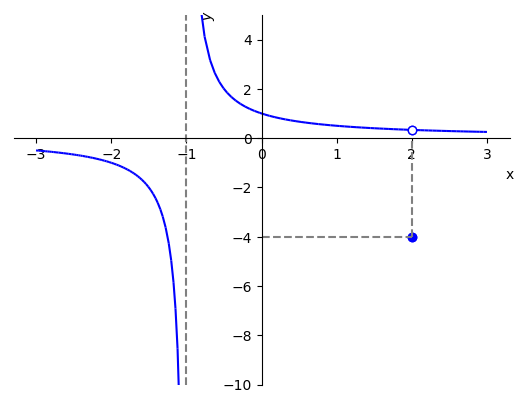
\includegraphics[width=0.7\textwidth]{./cap_lim/dados/fig_ex_conta/fig_ex_conta}
  \caption{Esboço do gráfico da função $f$ definida no Exemplo \ref{ex:conta}.}
  \label{fig:ex_conta}
\end{figure}

Vejamos a continuidade desta função nos seguintes pontos:
\begin{enumerate}[a)]
\item $x=-2$. Neste ponto, temos $f(-2) = -1$ e
  \begin{align}
    & \lim_{x\to -2} \frac{x-2}{(x+1)(x-2)} \\
    & \text{}\quad = \frac{-4}{-1\cdot(-4)} = -1 = f(-2).
  \end{align}
  Com isso, concluímos que $f$ é contínua no ponto $x=-2$.
\item $x=-1$. Neste ponto,
  \begin{align}
    & f(-1) = \frac{(x-2)}{(x+1)(x-2)} \\
    & \text{}\quad = \frac{1}{x-1} = \frac{1}{0}
  \end{align}
  logo, f(-1) não está definido e, portanto, $f$ é descontínua neste ponto. Observemos que $f$ tem uma assíntota vertical em $x=-1$, verifique!
\item $x=2$. Neste ponto, temos $f(2)=-4$ e
  \begin{align}
    & \lim_{x\to 2} \frac{x-2}{(x+1)(x-2)} \\
    & \text{}\quad = \lim_{x\to 2} \frac{1}{x+1} = \frac{1}{3} \neq f(2).
  \end{align}
  Portanto, concluímos que $f$ é descontínua em $x=2$.
\end{enumerate}
\end{ex}

Uma função $f$ é dita ser {\bf contínua em um intervalo} $(a, b)$, quando $f$ é contínua em todos os pontos $x_0\in (a, b)$. Para intervalos, $[a, b)$, $(a, b]$ ou $[a, b]$, empregamos a noção de continuidade lateral nos pontos de extremos fechados dos intervalos. Quando uma função é contínua em $(-\infty, \infty)$, dizemos que ela é {\bf contínua em toda parte}.

\begin{ex}\normalfont{(Continuidade da função valor absoluto.)}\label{ex:lim_fabs_cont}
  A função valor absoluto é contínua em toda parte. De fato, ela é definida por
  \begin{equation}
    |x| = \left\{
      \begin{array}{ll}
        x &, x\geq 0,\\
        -x &, x<0.
      \end{array}
    \right.
  \end{equation}
  Veja o esboço do gráfico desta função na Figura \ref{fig:funabs}.

  \begin{figure}[H]
    \centering
    \includegraphics[width=0.7\textwidth]{cap_lim/dados/fig_funabs/fig}
    \caption{Esboço do gráfico de $f(x) = |x|$.}
    \label{fig:funabs}
  \end{figure}
  
  Observamos que para $x\in(-\infty, 0)$ temos $|x| = x$ que é contínua para todos estes valores de $x$. Também, para $x\in(0,\infty)$ temos $|x|=-x$ que é contínua para todos estes valores de $x$. Agora, em $x=0$, temos $|0|=0$ e
  \begin{align}
    & \lim_{x\to 0^+} |x| = \lim_{x\to 0^+} x = 0, \\
    & \lim_{x\to 0^-} |x| = \lim_{x\to 0^-} -x = 0.
  \end{align}
  Logo,
  \begin{equation}
    \lim_{x\to 0} |x| = 0 = |0|.
  \end{equation}
  Com tudo isso, concluímos que a função valor absoluto é contínua em toda parte.
\end{ex}

\subsection{Propriedades de funções contínuas}

Se $f$ e $g$ são funções contínuas em $x=c_0$ e $k$ um número real, então também são contínuas em $x=x_0$ as funções:
\begin{enumerate}[a)]
\item $k\cdot f$
\item $f\pm g$
\item $f\cdot g$
\item $f/g$, se $g(x_0)\neq 0$
\item $f^k$, se existe $f^k(x_0)$.
\end{enumerate}

\begin{ex}
  Temos que $f(x) = x$ e $g(x) = |x|$ são exemplos de funções contínuas em toda parte. Segue das propriedades acima que:
  \begin{enumerate}[a)]
  \item $f_a(x) = 2x$ é contínua em toda parte.
  \item $f_b(x) = x + |x|$ é contínua em toda parte.
  \item $f_c(x) = 2x|x|$ é contínua em toda parte.
  \item $f_d(x) = \frac{|x|}{x}$ é contínua para todo $x\in\mathbb{R}\setminus\{0\}$.
  \item $f_e(x) = x^2$ é contínua em toda parte.
  \end{enumerate}
\end{ex}

\begin{ex}
  {\bf Polinômios são contínuos em toda parte}. Isto é, se $p(x) = a_nx^n+a_{n-1}x^{n-1}+\cdots+a_1x+a_0$, então
  \begin{equation}
    \lim_{x\to x_0} p(x) = p(x_0),
  \end{equation}
  para qualquer $x_0\in\mathbb{R}$. Por exemplo,
  \begin{equation}
    \lim_{x\to -1} 2 - x^2 + x^5 = 2 - (-1)^2 + (-1)^5 = 0.
  \end{equation}
\end{ex}

\begin{ex}
  {\bf Funções racionais $r(x) = p(x)/q(x)$ são contínuas em todos os pontos de seus domínios}. Por exemplo, a função racional
  \begin{equation}
    f(x) = \frac{x-1}{x^2-1},
  \end{equation}
  é descontínua nos pontos
  \begin{equation}
    x^2-1 = 0 \Rightarrow x = \pm 1,
  \end{equation}
  pois $f$ não está definida nestes pontos. Agora, para $x_0\neq 1$ e $x_0\neq -1$, temos
  \begin{align}
    & \lim_{x\to x_0} f(x) \\
    & \text{}\quad = \lim_{x\to x_0} \frac{x-1}{x^2-1} \\
    & \text{}\quad = \frac{x_0-1}{x_0^2-1} = f(x_0).
  \end{align}
  Por exemplo,
  \begin{equation}
    \lim_{x\to 0} f(x) = \frac{0-1}{0^2-1} = 1 = f(0).
  \end{equation}
  Ou seja, $f$ é contínua nos intervalos $(-\infty, -1) \cup (-1, 1) \cup (1, \infty)$, que coincide com seu domínio.
\end{ex}

\begin{obs}
  São contínuas em todo seu domínio as funções potência, polinomiais, racionais, trigonométricas, exponenciais e logarítmicas.
\end{obs}

Se $f$ é contínua no ponto $x_0$ e $g$ é contínua no ponto $f(x_0)$, então $g\circ f$ é contínua no ponto $x_0$.

\begin{ex}
  Vejamos os seguintes casos:
  \begin{enumerate}[a)]
  \item $y = \sqrt{x^2-1}$ é descontínua nos pontos $x$ tais que
    \begin{equation}
      x^2-1<0\Rightarrow -1<x<1.
    \end{equation}
    Isto é, esta função é contínua em $(-\infty,-1]\cup[1,\infty)$.
  \item $\displaystyle y = \left|\frac{x-1}{x^2-1}\right|$ é descontínua nos pontos $x$ tais que
    \begin{equation}
      x^2-1=0\Rightarrow x=\pm 1.
    \end{equation}
  \end{enumerate}
\end{ex}

\begin{ex}
  Podemos explorar a continuidade para calcularmos limites. Por exemplo,
  \begin{equation}
    \lim_{x\to 0} \sqrt{x+4}\cdot e^{\sen x} = \sqrt{\lim_{x\to 0} x+4}\cdot e^{\sen \lim_{x\to 0} x} = \sqrt{4}\cdot e^{0} = 2.
  \end{equation}
\end{ex}

\subsubsection{Teorema do Valor Intermediário}

O Teorema do Valor Intermediário estabelece que qualquer dada função $f$ contínua em um intervalo $[a, b]$, assume todos os valores entre $f(a)$ e $f(b)$. Consulte a Figura \ref{fig:teo_valorint}.

\begin{figure}[H]
  \centering
  \includegraphics[width=0.7\textwidth]{cap_lim/dados/fig_teo_valorint/fig}
  \caption{Ilustração sobre o Teorema do Valor Intermediário.}
  \label{fig:teo_valorint}
\end{figure}

\begin{teo}\normalfont{(Teorema do valor intermediário)}\label{teo:valorintermediario}
  Seja $f$ função contínua em um intervalo fechado $[a, b]$. Se $d$ é um número entre $f(a)$ e $f(b)$, então existe $c\in [a, b]$ tal que $f(c)=d$.
\end{teo}



\begin{ex}
  Podemos afirmar que $f(x)=x^3-x-1$ tem (pelo menos) um zero no intervalo $(0, 2)$. De fato, $f$ é contínua no intervalo $[0,2]$ e, pelo teorema do valor intermediário, assume todos os valores entre $f(0)=-1<0$ e $f(2)=5>0$. Observemos que $y = 0$ está entre $f(0)$ e $f(2)$. Veja a Figura \ref{fig:cap_lim_ex_teoint}.

  \begin{figure}[H]
    \centering
    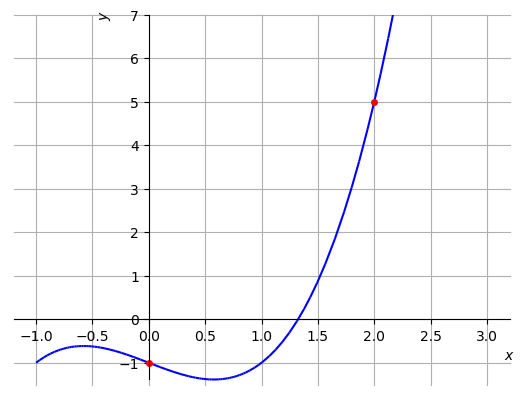
\includegraphics[width=0.7\textwidth]{./cap_lim/dados/fig_cap_lim_ex_teoint/fig_cap_lim_ex_teoint}
    \caption{Esboço do gráfico da função $f(x) = x^3-x-1$.}
    \label{fig:cap_lim_ex_teoint}
  \end{figure}
\end{ex}

\subsection{Exercícios resolvidos}

% \begin{flushright}
%   [Vídeo] | [Áudio] | \href{https://phkonzen.github.io/notas/contato.html}{[Contatar]}
% \end{flushright}

\begin{exeresol}
  Encontre os pontos de continuidade da função
  \begin{equation}
    f(x) = \frac{|x|}{x}.
  \end{equation}
\end{exeresol}
\begin{resol}
  Observamos que a função é descontínua em $x=0$, pois não está definida neste ponto. Agora, para $x < 0$, temos
  \begin{equation}
    f(x) = \frac{|x|}{x} = \frac{-x}{x} = -1.
  \end{equation}
  Ou seja, para $x<0$ a função é constante igual a $-1$ e, portanto, contínua.

  Para $x > 0$, temos
  \begin{equation}
    f(x) = \frac{|x|}{x} = \frac{x}{x} = 1.
  \end{equation}
  I.e., para $x > 0$ a função é constante igual a $1$ e, portanto, contínua.

  Concluímos que $f(x)$ é contínua em $\mathbb{R}\setminus\{0\}$. Faça o esboço do gráfico desta função!
\end{resol}

\begin{exeresol}
  Encontre os pontos de continuidade da função
  \begin{equation}
    f(x) = \ln\left(\frac{x+1}{x-1}\right).
  \end{equation}
\end{exeresol}
\begin{resol}
  A função $f$ pode ser vista como a composição da função logaritmo natural $g(x) = \ln x$ com a função racional $\displaystyle h(x) = \frac{x+1}{x-1}$. Observamos que:
  \begin{enumerate}[a)]
  \item a função logaritmo natural é contínua em todo o seu domínio, i.e. $g$ é contínua para todo $x > 0$;
  \item a função racional $\displaystyle h(x) = \frac{x+1}{x-1}$ é contínua para todo $x\neq 1$.
  \end{enumerate}
  Lembrando que a composição de funções contínuas é contínua, temos que a função $f(x) = g(h(x))$ é contínua nos pontos de continuidade da função $h$ tais que $h(x) > 0$, i.e. para $x\neq 1$ e
  \begin{equation}
    \frac{x+1}{x-1} > 0.
  \end{equation}
  Fazendo o estudo de sinal
  \begin{center}
    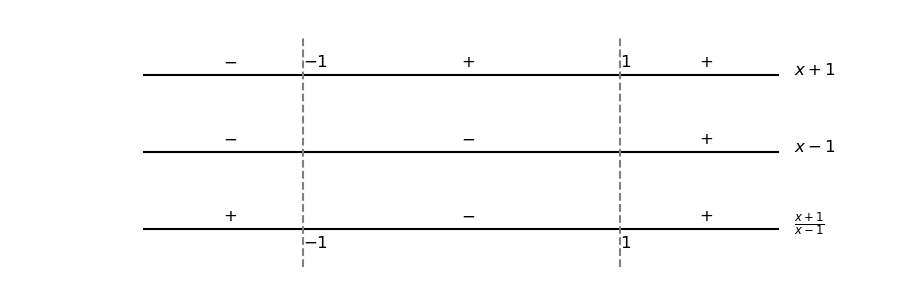
\includegraphics[width=0.8\textwidth]{./cap_lim/dados/fig_cap_lim_exeresol_estsinal/fig_cap_lim_exeresol_estsinal}
  \end{center}
  vemos que $h(x) > 0$ em $(-\infty, -1)\cup (1, \infty)$.

  Em resumo, $h$ é contínua em $(0, \infty)$ e $g$ é contínua e positiva em $(-\infty, -1)\cup (1, \infty)$. A função $f = (h\circ g)$ é contínua na interseção destes conjuntos, i.e. $f$ é contínua em $(1, \infty)$. 
\end{resol}

\subsection{Exercícios}


\begin{exer}
  Encontre os pontos de continuidade da função
  \begin{equation}
    f(x) = \frac{x^3 - 27}{x^2 - 3x + 2}.
  \end{equation}
\end{exer}
\begin{resp}
  $\mathbb{R}\setminus\{1,2\}$.
\end{resp}

\begin{exer}
  Encontre os pontos de continuidade da função
  \begin{equation}
    f(x) = \sqrt{\frac{x^3 - 27}{x^2 - 3x + 2}}.
  \end{equation}
\end{exer}
\begin{resp}
  $(1, 2)\cup (3, \infty)$.
\end{resp}

\begin{exer}
  Calcule
  \begin{enumerate}[a)]
  \item $\displaystyle\lim_{x\to -1}e^{x^2-1}$
  \item $\displaystyle\lim_{x\to \sqrt{2}}\ln |x^2-1|$
  \end{enumerate}
\end{exer}
\begin{resp}
  a) $1$; b) $0$
\end{resp}

\begin{exer}
  Calcule
  \begin{equation}
    \lim_{x\to \pi} \ln \left(\frac{\sen \frac{x}{2} - \cos x}{2}\right).
  \end{equation}
\end{exer}
\begin{resp}
  $0$
\end{resp}

\begin{exer}
  Calcule o valor de $c$ de forma que a seguinte função seja contínua em $x=1$.
  \begin{equation}
    f(x) = \left\{
      \begin{array}{ll}
        \frac{x-1}{x^2-1} &, x\neq 1\\
        c &, x=1
      \end{array}\right.
  \end{equation}
\end{exer}
\begin{resp}
  $c=\frac{1}{2}$
\end{resp}

\begin{exer}(Aplicação.)
  O fenômeno de desintegração espontânea do núcleo de um átomo com a emissão de algumas radiações é chamado de radioatividade\footnote{Fonte: \href{https://pt.wikipedia.org/wiki/Radioatividade}{Wikipédia}.}. A lei fundamental do decaimento radiativo estabelece que a taxa de decaimento é proporcional ao número de átomos que ainda não decaíram. Isto nos fornece a equação da lei básica da radioatividade
  \begin{equation}
    N = N_0e^{-\lambda t}
  \end{equation}
  onde, $N = N(t)$ é o número de átomos no tempo $t$, $N_0\geq 0$ é o número de átomos presentes no tempo inicial $t=0$ e $\lambda>0$ é a constante de decaimento. Qual a tendência de $N = N(t)$ quando a taxa de decaimento $\lambda\to 0^+$.
\end{exer}
\begin{resp}
  $N(t)\to N_0$ quando $\lambda\to 0^+$
\end{resp}

\ifisbook
\subsubsection{Respostas}
\shipoutAnswer
\fi

\section{Limites e desigualdades}\label{cap_lim_sec_limdes}

Se $f$ e $g$ são funções tais que $f(x){\color{blue}<}g(x)$ para todo $x$ em um certo intervalo aberto contendo $x_0$, exceto possivelmente em $x=x_0$, e existem os limites de $f$ e $g$ no ponto $x=x_0$, então
\begin{equation}
  \lim_{x\to x_0} f(x) {\color{blue}\leq} \lim_{x\to x_0} g(x).
\end{equation}
Observe que a tomada do {\bf limite não preserva a desigualdade estrita}.

\begin{ex}
  As funções $f(x) = x^2/3$ e $g(x) = x^2/2$ são tais que $f(x) < g(x)$ para todo $x\neq 0$. Ainda, temos
  \begin{equation}
    \lim_{x\to 0} f(x) = 0\quad\text{e}\quad\lim_{x\to 0} g(x) = 0.
  \end{equation}
\end{ex}

\begin{obs}
  A preservação da desigualdade também ocorre para limites laterais. Mais precisamente, se $f$ e $g$ são funções tais que $f(x)<g(x)$ para todo $x < x_0$ e existem os limites laterais à esquerda de $f$ e $g$ no ponto $x=x_0$, então
  \begin{equation}
    \lim_{x\to x_0^-} f(x) \leq \lim_{x\to x_0^-} g(x).
  \end{equation}
  Vale o resultado análogo para limite lateral à direita e limites no infinito.
\end{obs}

\subsection{Limites de funções limitadas}

\begin{flushright}
  [Vídeo] | [Áudio] | \href{https://phkonzen.github.io/notas/contato.html}{[Contatar]}
\end{flushright}

Se $f(x) \leq L$ para todo $x$ em um intervalo aberto contendo $x_0$, exceto possivelmente em $x_0$, então
\begin{equation}
  \lim_{x\to x_0} f(x) \leq L.
\end{equation}
Resultados análogos valem para limites laterais e limites no infinito.

\begin{ex}
  Vamos calcular o seguinte limite
  \begin{equation}
    \lim_{x\to \infty} e^{-x}\sen x.
  \end{equation}

  
  
  Como $|\sen x| \leq 1$, temos
  \begin{align}
    & \lim_{x\to \infty} e^{-x}\sen x \leq \lim_{x\to \infty} e^{-x} = 0,\\
    & \lim_{x\to \infty} e^{-x}\sen x \geq \lim_{x\to \infty} -e^{-x} = 0.
  \end{align}
  Logo, temos
  \begin{equation}
    \lim_{x\to \infty} e^{-x}\sen x = 0.
  \end{equation}
\end{ex}


\subsection{Teorema do confronto}

% \begin{flushright}
%   [YouTube] | [Vídeo] | [Áudio] | \href{https://phkonzen.github.io/notas/contato.html}{[Contatar]}
% \end{flushright}

\begin{teo}\normalfont{(Teorema do confronto)}\label{teo:confronto}
  Se $g(x) \leq f(x) \leq h(x)$ para todo $x$ em um intervalo aberto contendo $a$, exceto possivelmente em $x=a$ (consulte a Figura \ref{fig:limSanduiche}), e
  \begin{equation}
    \lim_{x\to a} g(x) = \lim_{x\to a} h(x) = L,
  \end{equation}
  então
  \begin{equation}
    \lim_{x\to a} f(x) = L.
  \end{equation}
\end{teo}

\begin{figure}[H]
  \centering
  \includegraphics[width=0.7\textwidth]{./cap_lim/dados/figLimSanduiche/fig}
  \caption{Ilustração sobre o Teorema \ref{teo:confronto}.}
  \label{fig:limSanduiche}
\end{figure}

\begin{dem}
  Da preservação da desigualdade, temos
  \begin{equation}
    \lim_{x\to a} g(x) \leq \lim_{x\to a} f(x) \leq \lim_{x\to a} h(x)
  \end{equation}
  donde
  \begin{equation}
    L \leq \lim_{x\to a} f(x) \leq L.
  \end{equation}
\end{dem}

\begin{ex}
  Toda função $f(x)$ tal que $-1+x^2/2 \leq f(x) \leq -1+x^2/3$, para todo $x\neq 0$, tem
  \begin{equation}
    \lim_{x\to 0} f(x) = -1.
  \end{equation}
\end{ex}

\begin{obs}
  O Teorema do confronto também se aplica a limites laterais.
\end{obs}

\begin{ex}\label{ex:senx}
  \begin{equation}
    \lim_{x\to 0} \sen x = 0.
  \end{equation}

  \begin{figure}[H]
    \centering
    \includegraphics[width=0.7\textwidth]{./cap_lim/dados/figLimSenx/fig}
    \caption{Ilustração referente ao Exemplo \ref{ex:senx}.}
    \label{fig:limSenx}
  \end{figure}
  
  De fato, começamos assumindo $0<x<\pi/2$. Tomando $O = (0,0)$, $A=(1,0)$ e $P = (\cos x, \sen x)$ (consulte a Figura \ref{fig:limSenx}), observamos que
  \begin{equation}
    \text{Área do triâng.} OAP < \text{Área do setor} OAP,
  \end{equation}
  i.e.
  \begin{equation}
    \frac{\sen x}{2} < \frac{x}{2} \Rightarrow \sen x < x,
  \end{equation}
  para todo $0< x < \pi/2$. 

  É certo que $\sen x < -x$ para $-\pi/2 < x < 0$. Com isso e o resultado acima, temos
  \begin{equation}\label{eq:senx0}
    \sen x \leq |x|,\quad -\pi/2 < x < \pi/2.
  \end{equation}

  Lembrando que $\sen x$ é uma função ímpar, temos
  \begin{equation}\label{eq:senx1}
    -|x| \leq -\sen x = \sen -x,\quad -\pi/2 < x < \pi/2.
  \end{equation}
  Logo, de \eqref{eq:senx0} e \eqref{eq:senx1}, temos
  \begin{equation}
    -|x| \leq \sen x \leq |x|.
  \end{equation}

  Por fim, como
  \begin{equation}
    \lim_{x\to 0} -|x| = \lim_{x\to 0} |x| = 0,
  \end{equation}
  do Teorema do confronto, concluímos
  \begin{equation}
    \lim_{x\to 0} \sen x = 0.
  \end{equation}
\end{ex}

\begin{obs}
  Do exemplo anterior (Exemplo \ref{ex:senx}), podemos mostrar que
\begin{equation}
  \lim_{x\to 0} \cos x = 1.
\end{equation}

De fato, da identidade trigonométrica de ângulo metade
\begin{equation}
  \sen^2 \frac{x}{2} = \frac{1 - \cos x}{2}
\end{equation}
temos
\begin{equation}
  \cos x = 1 + 2\sen^2 \frac{x}{2}.
\end{equation}
Então, aplicando as regras de cálculo de limites, obtemos
\begin{align}
  & \lim_{x\to 0} \cos x = \lim_{x\to 0} \left[1 + 2\sen^2 \frac{x}{2}\right] \\
  & \text{}\quad = 1 + 2\left(\lim_{x\to 0} \sen \frac{x}{2}\right)^2.\label{eq:senx2}
\end{align}
Agora, fazemos a mudança de variável $y = x/2$. Neste caso, temos $y\to 0$ quando $x\to 0$ e, então
\begin{equation}
  \lim_{x\to 0} \sen \frac{x}{2} = \lim_{y\to 0} \sen y = 0.
\end{equation}
Então, retornando a equação \eqref{eq:senx2}, concluímos
\begin{equation}
  \lim_{x\to 0} \cos x = 1.
\end{equation}
\end{obs}

\subsection{Limites envolvendo $(\sen x)/x$}\label{sec:lim_senx_x}

\begin{flushright}
  [Vídeo] | [Áudio] | \href{https://phkonzen.github.io/notas/contato.html}{[Contatar]}
\end{flushright}

Verificamos o seguinte resultado
\begin{equation}\label{eq:lim_senx_x}
  \lim_{x\to 0} \frac{\sen x}{x} = 1.
\end{equation}

\begin{figure}[H]
  \centering
  \includegraphics[width=0.7\textwidth]{./cap_lim/dados/figLimSenxOx/fig}
  \caption{Ilustração para o cálculo de $\displaystyle\lim_{x\to 0}\frac{\sen x}{x}$.}
  \label{fig:limSenxOx}
\end{figure}

Para verificarmos este resultado, calcularemos os limites laterais à esquerda e à direita. Começamos com o limite lateral a direita e assumimos $0<x<\pi/2$. Sendo os pontos $O=(0,0)$, $P=(\cos x,\sen x)$, $A = (1,0)$ e $T = (1, \tg x)$ (consulte Figura \ref{fig:limSenxOx}), observamos que
\begin{equation}
  \text{Área do triâng. } OAP < \text{Área do setor} OAP < \text{Área do triâng. } OAT.
\end{equation}
Ou seja, temos
\begin{equation}
  \frac{\sen x}{2} < \frac{x}{2} < \frac{\tg x}{2}.
\end{equation}
Multiplicando por $2$ e dividindo por $\sen x$\footnote{$\sen x > 0$ para todo $0< x < \pi/2$.}, obtemos
\begin{equation}
  1 < \frac{x}{\sen x} < \frac{1}{\cos x}.
\end{equation}
Tomando os recíprocos, temos
\begin{equation}
  1 > \frac{\sen x}{x} > \cos x.
\end{equation}
Agora, passando ao limite
\begin{equation}
  1 = \lim_{x\to 0^+} 1 \geq \lim_{x\to 0^+} \frac{\sen x}{x} \geq \lim_{x\to 0^+} \cos x = 1.
\end{equation}
Logo, concluímos que
\begin{equation}
  \lim_{x\to 0^+} \frac{\sen x}{x} = 1.
\end{equation}

Agora, usando o fato de que $\sen x/x$ é uma função par, temos
\begin{align}
  & \lim_{x\to 0^-} \frac{\sen x}{x} = \lim_{x\to 0^-} \frac{\sen(-x)}{-x} \\
  & \text{}\quad = \lim_{x\to 0^+} \frac{\sen x}{x} = 1.
\end{align}

Calculados os limites laterais, concluímos o que queríamos.

\begin{ex}
  Com o resultado acima e as regras de cálculo de limites, temos
  \begin{equation}
    \lim_{x\to 0} \frac{\cos(x) - 1}{x} = 0.
  \end{equation}
  Veja o Exercício \ref{exer:lim_cosx_1}.
\end{ex}

\subsection{Exercícios resolvidos}

% \begin{flushright}
%   [Vídeo] | [Áudio] | \href{https://phkonzen.github.io/notas/contato.html}{[Contatar]}
% \end{flushright}

\begin{exeresol}
  Sabendo que $x^3 \leq f(x) \leq \sqrt{x}$ para $0 < x < 1$, calcule
  \begin{equation}
    \lim_{x\to 0^+} f(x).
  \end{equation}
\end{exeresol}
\begin{resol}
  Pelo Teorema do Confronto, temos
  \begin{equation}
    \lim_{x\to 0^+} \cancelto{0}{x^3} \leq \lim_{x\to 0^+} f(x) \leq \lim_{x\to 0^+} \cancelto{0}{\sqrt{x}}.
  \end{equation}
  Logo,
  \begin{equation}
    \lim_{x\to 0^+} f(x) = 0.
  \end{equation}
\end{resol}


\subsection{Exercícios}


\begin{exer}
  Supondo que $1-x^2/3 \leq u(x) \leq 1-x^2/2$ para todo $x\neq 0$, determine o $\lim_{x\to 0} u(x)$.
\end{exer}
\begin{resp}
  $1$
\end{resp}

\begin{exer}
  Calcule
  \begin{equation}
    \lim_{x\to \infty} e^{-x}\cos x.
  \end{equation}
\end{exer}
\begin{resp}
  $0$
\end{resp}

\begin{exer}
  Calcule
  \begin{equation}
    \lim_{x\to 0} \frac{\sen 3x}{6x}.
  \end{equation}
\end{exer}
\begin{resp}
  $\frac{1}{2}$
\end{resp}

\begin{exer}\label{exer:lim_cosx_1}
  Calcule
  \begin{equation}
    \lim_{x\to 0} \frac{\cos(x)-1}{x}.
  \end{equation}
\end{exer}
\begin{resp}
  $0$
\end{resp}

\begin{exer}
  Calcule
  \begin{equation}
    \lim_{x\to 0} \frac{\cos(3x)-1}{6x}.
  \end{equation}
\end{exer}
\begin{resp}
  $0$
\end{resp}

\section{Exercícios finais}\label{cap_lim_sec_exfinal}

\begin{flushright}
  [Vídeo] | [Áudio] | \href{https://phkonzen.github.io/notas/contato.html}{[Contatar]}
\end{flushright}

\begin{exer}
  Calcule
  \begin{equation}
    \lim_{x\to 1^+} \ln\left(\frac{x+1}{x-1}\right).
  \end{equation}
\end{exer}
\begin{resp}
  $\infty$
\end{resp}

\begin{exer}
  Calcule os seguintes limites:
  \begin{enumerate}[a)]
  \item $\displaystyle\lim_{x\to\infty} x^x$
  \item $\displaystyle\lim_{x\to\infty} \left(\frac{1}{x}\right)^x$
  \end{enumerate}
\end{exer}
\begin{resp}
  a)~$\infty$; b)~$0$
\end{resp}

\ifisbook
\subsubsection{Respostas}
\shipoutAnswer
\fi
%Este trabalho está licenciado sob a Licença Atribuição-CompartilhaIgual 4.0 Internacional Creative Commons. Para visualizar uma cópia desta licença, visite http://creativecommons.org/licenses/by-sa/4.0/deed.pt_BR ou mande uma carta para Creative Commons, PO Box 1866, Mountain View, CA 94042, USA.

\chapter{Derivadas}\label{cap_deriv}
\thispagestyle{fancy}

\section{Derivada no ponto}\label{cap_deriv_sec_derivpt}

Nesta seção, vamos estudar a noção de {\bf derivada de uma função em um ponto}. Começamos pelas noções de {\bf reta secante} e de {\bf reta tangente} ao gráfico de uma função. Em seguida, estudamos as noções de {\bf taxa de variação média} e {\bf taxa de variação instantânea}. Por fim, definimos a derivada de uma função em um ponto.

\subsection{Reta secante e reta tangente}

\begin{flushright}
  [YouTube] | [Vídeo] | [Áudio] | \href{https://phkonzen.github.io/notas/contato.html}{[Contatar]}
\end{flushright}

Definimos a {\bf reta secante} ao gráfico de uma dada função $f$ pelos pontos $x_0$ e $x_1$, $x_0\neq x_1$, como sendo a reta determinada pela equação
\begin{equation}
  {\color{blue}y = \frac{f(x_1)-f(x_0)}{x_1-x_0}(x-x_0)+f(x_0)}.
\end{equation}
Isto é, é a reta que passa pelos pontos $(x_0,f(x_0))$ e $(x_1,f(x_1))$. Veja a Figura \ref{fig:retsectg}. Observemos que o coeficiente angular da reta secante é
\begin{equation}
  {\color{blue}m_{\text{sec}} = \frac{f(x_1)-f(x_0)}{x_1-x_0}}.
\end{equation}

\begin{figure}[H]
  \centering
  \includegraphics[width=0.8\textwidth]{./cap_deriv/dados/fig_retsectg/fig}
  \caption{Esboços de uma reta secante (verde) e da reta tangente (vermelho) ao gráfico de uma função.}
  \label{fig:retsectg}
\end{figure}

A {\bf reta tangente} ao gráfico de uma função $f$ em $x=x_0$ é a reta que passa pelo ponto $(x_0, f(x_0))$ e tem coeficiente angular
\begin{equation}\label{eq:mtg}
  {\color{blue}m_{\text{tg}} = \lim_{x_1\to x_0} \frac{f(x_1)-f(x_0)}{x_1-x_0}}.
\end{equation}
Isto é, a reta de equação
\begin{equation}
  {\color{blue}y = m_{\text{tg}}(x-x_0)+f(x_0)}.
\end{equation}
Menos formal, é a reta limite das retas secantes ao gráfico da função pelos pontos $x_0$ e $x_1$, quando $x_1\to x_0$. Veja a Figura \ref{fig:retsectg}.

\begin{obs}
  Fazendo a mudança de variável $h = x_1-x_0$, temos que \eqref{eq:mtg} é equivalente a
  \begin{equation}
    {\color{blue}m_{\text{tg}} = \lim_{h\to 0} \frac{f(x_0+h)-f(x_0)}{h}}.
  \end{equation}
  De fato, da mudança de variável, temos que $x_1 = x_0+h$ e quando $x_1\to x_0$, temos que $h = x_1-x_0\to 0$. Ou seja,
  \begin{align}
    m_{\text{tg}} &= \lim_{x_1\to x_0} \frac{f(x_1)-f(x_0)}{x_1-x_0}\\
                  &= \lim_{h\to 0} \frac{f(x_0+h)-f(x_0)}{h}.
  \end{align}
\end{obs}

\begin{ex}
  Seja $f(x)=x^2$ e $x_0 = 1$. O coeficiente angular da reta secante ao gráfico de $f$ pelos pontos $x_0=1$ e $x_1 = 2$ é
  \begin{align}
    m_{\text{sec}} &= \frac{f(x_1)-f(x_0)}{x_1-x_0}\\
                   &= \frac{f(2) - f(1)}{2-1}\\
                   &= \frac{4-1}{1} = 3.
  \end{align}
  Logo, a reta secante ao gráfico de $f$ pelos pontos $x_0=1$ e $x_1=2$ tem equação
  \begin{gather}
    y = m_{\text{sec}}(x-x_0) + f(x_0) \\
    y = 3(x-1)+f(1) \\
    y = 3x - 2.
  \end{gather}
  Na Figura \ref{fig:cap_deriv_ex_rt_x2}, temos os esboços dos gráfico da função e da reta secante (verde).
  
  \begin{figure}[H]
    \centering
    \includegraphics[width=0.7\textwidth]{./cap_deriv/dados/fig_cap_deriv_ex_rt_x2/fig}
    \caption{Esboços dos gráficos de $f(x)=x^2$ (azul), da reta secante pelos pontos $x_0=1$ e $x_1=2$ (verde) e da reta tangente ao gráfico de $f$ no ponto $x_0 = 1$ (vermelho).}
    \label{fig:cap_deriv_ex_rt_x2}
  \end{figure}

  Agora, o coeficiente angular da reta tangente ao gráfico de $f$ no ponto $x_0$ é
  \begin{align}
    m_{\text{tg}} &= \lim_{h\to 0} \frac{f(x_0+h)-f(x_0)}{h}\\
                  &= \lim_{h\to 0} \frac{(1+h)^2-1}{h}\\
                  &= \lim_{h\to 0} \frac{1+2h+h^2-1}{h}\\
                  &= \lim_{h\to 0} \frac{2+h}{1} = 2.
  \end{align}
  Assim sendo, a reta tangente ao gráfico de $f(x)=x^2$ no ponto $x_0=1$ tem coeficiente angular $m_{\text{tg}} = 2$ e equação
  \begin{equation}
    y = 2(x-1)+1 = 2x-1.
  \end{equation}
  Na Figura \ref{fig:cap_deriv_ex_rt_x2}, temos os esboços dos gráfico da função e da reta tangente (vermelho).
  
  \ifispython
  Com o {\python}+{\sympy}, podemos obter a expressão da reta secante com os seguintes comandos:
  \begin{lstlisting}
    In : from sympy import *
    ...: x,y = symbols('x,y')
    ...: x0 =  1
    ...: x1 = 2
    ...: f = lambda x: x**2
    ...: msec = (f(x1)-f(x0))/(x1-x0)
    ...: Eq(y, msec*(x-x0)+f(x0))
    Out: Eq(y, 3.0*x - 2.0)
  \end{lstlisting}
  A expressão da reta tangente pode ser obtida com os seguintes comandos:
  \begin{lstlisting}
    In : from sympy import *
    ...: x,y = symbols('x,y')
    ...: h = Symbol('h')
    ...: x0 = 1
    ...: f = lambda x: x**2
    ...: mtg = limit((f(x0+h)-f(x0))/h, h, 0)
    ...: Eq(y, mtg*(x-x0)+f(x0))
    ...: 
    Out: Eq(y, 2*x - 1)
  \end{lstlisting}
  \fi
\end{ex}

\subsection{Taxa de variação}

\begin{flushright}
  [YouTube] | [Vídeo] | [Áudio] | \href{https://phkonzen.github.io/notas/contato.html}{[Contatar]}
\end{flushright}

A {\bf taxa de variação média} de uma função $f$ quando $x$ varia de $x_0$ a $x_1$ é definida como
\begin{equation}
  \frac{\Delta y}{\Delta x} := \frac{f(x_1)-f(x_0)}{x_1-x_0}. 
\end{equation}
Desta deriva-se a {\bf taxa de variação instantânea} de $f$ no ponto $x_0$, a qual é definida como
\begin{align}
  \left.\frac{\dd f}{\dd x}\right|_{x=x_0} &:= \lim_{x\to x_0} \frac{f(x)-f(x_0)}{x-x_0}\\
                             &= \lim_{h\to 0} \frac{f(x_0+h)-f(x_0)}{h}.
\end{align}
Em muitas áreas do conhecimento, estas taxa recebem nomes específicos.

\begin{ex}
  Seja $s = s(t)$ a função distância percorrida por um objeto no tempo. A {\bf velocidade média} (taxa de variação média da distância) do tempo $t_0$ ao tempo $t_1$ é
  \begin{equation}
    \frac{\Delta s}{\Delta t} = \frac{s(t_1)-s(t_0)}{t_1-t_0}.
  \end{equation}
  Por exemplo, se $s(t) = 15t^2+t$ (km), então a velocidade média do objeto entre $t_0=1$h e $t_1=3$h é
  \begin{align}
    \frac{\Delta s}{\Delta t} &= \frac{(15t_1^2+t_1)-(15t_0^2+t_0)}{t_1-t_0}\\
                              &= \frac{15\cdot 3^2+3-(15\cdot 1^2+1)}{3-1}\\
                              &= \frac{135+3-15-1}{2}\\
                              &= 61~\frac{\text{km}}{\text{h}}.
  \end{align}

  A {\bf velocidade} (taxa de variação instantânea da distância) no tempo $t_0=1$ é
  \begin{align}
    \left.\frac{\dd s}{\dd t}\right|_{t=t_0} &= \lim_{h\to 0} \frac{s(t_0+h)-s(t_0)}{h} \\
                                             &= \lim_{h\to 0} \frac{15(t_0+h)^2+(t_0+h)-\left(15t_0^2+t_0\right)}{h}\\
                                             &= \lim_{h\to 0} \frac{15t_0^2+30t_0h+15h^2+t_0+h-15t_0^2-t_0}{h}\\
                                             &= \lim_{h\to 0} \frac{30t_0h+15h^2+h}{h}\\
                                             &= \lim_{h\to 0} 30t_0 + 15h + 1 \\
                                             &= 30t_0+1 = 31~\frac{\text{km}}{\text{h}}.
  \end{align}
\end{ex}

\begin{ex}
  Seja $c(x) = \sqrt{x}$ (milhões de reais) o custo da produção em uma empresa em função do número de unidades produzidas (milhares). O {\bf custo médio da produção} de $x_0=4$ a $x_1=9$ é
  \begin{align}
    \frac{\Delta c}{\Delta x} &= \frac{c(x_1)-c(x_0)}{x_1-x_0}\\
                              &= \frac{\sqrt{x_1}-\sqrt{x_0}}{x_1-x_0}\\
                              &= \frac{\sqrt{9}-\sqrt{4}}{9-4}\\
                              &= \frac{3-2}{5} \\
                              &= 0,2~\frac{\text{R\$}}{\text{un}}.
  \end{align}

  O {\bf custo marginal} (taxa de variação instantânea do custo) quando a empresa está produzindo $x_0=4$ milhões de unidades é
  \begin{align}
    \left.\frac{\dd c}{\dd x}\right|_{x=x_0=4} &= \lim_{h\to 0} \frac{\sqrt{x_0+h}-\sqrt{x_0}}{h}\\
                                               &= \lim_{h\to 0} \frac{\sqrt{x_0+h}-\sqrt{x_0}}{h}\cdot \frac{\sqrt{x_0+h}+\sqrt{x_0}}{\sqrt{x_0+h}+\sqrt{x_0}}\\
                                               &= \lim_{h\to 0} \frac{x_0+h-x_0}{h(\sqrt{x_0+h}+\sqrt{x_0})}\\
                                               &= \lim_{h\to 0} \frac{1}{\sqrt{x_0+\cancelto{0}{h}}+\sqrt{x_0}}\\
                                               &= \frac{1}{2\sqrt{x_0}} = \frac{\sqrt{x_0}}{2x_0}\\
                                               &= \frac{\sqrt{4}}{2\cdot 4} = 0,25~\frac{\text{R\$}}{\text{un}}.
  \end{align}
\end{ex}

\begin{obs}
  Analogamente a custo marginal, temos as noções de rendimento marginal e lucro marginal.
\end{obs}

\subsection{Derivada em um ponto}

\begin{flushright}
  [Vídeo] | [Áudio] | \href{https://phkonzen.github.io/notas/contato.html}{[Contatar]}
\end{flushright}

A {\bf derivada} de uma função $f$ {\bf em um ponto} $x=x_0$ é denotada por $f'(x_0)$ ou $\displaystyle \frac{\dd f}{\dd x}(x_0)$ e é definida por
\begin{equation}
  f'(x_0) = \left.\frac{\dd f}{\dd x}\right|_{x=x_0} := \lim_{h\to 0} \frac{f(x_0+h)-f(x_0)}{h}.
\end{equation}

\begin{ex}
  Vejamos os seguintes casos:
  \begin{enumerate}[a)]
  \item $f(x) = k$, $k$ constante.
    \begin{align}
      f'(x_0) &= \lim_{h\to 0} \frac{f(x_0+h)-f(x_0)}{h}\\
              &= \lim_{h\to 0} \frac{k-k}{h} = 0.
    \end{align}
  \item $f(x) = x$.
    \begin{align}
      f'(x_0) &= \lim_{h\to 0} \frac{f(x_0+h)-f(x_0)}{h} \\
              &= \lim_{h\to 0} \frac{x_0+h-x_0}{h} = 1.
    \end{align}
  \item $f(x) = \sqrt{x}$, $x_0=1$.
    \begin{align}
      f'(1) &= \lim_{h\to 0} \frac{\sqrt{1+h}-\sqrt{1}}{h}\\
            &= \lim_{h\to 0} \frac{\sqrt{1+h}-\sqrt{1}}{h} \cdot \frac{\sqrt{1+h}+\sqrt{1}}{\sqrt{1+h}+\sqrt{1}}\\
            &= \lim_{h\to 0} \frac{1+h-1}{h(\sqrt{1+h}+1)} = \frac{1}{2}.
    \end{align}
  \end{enumerate}
\end{ex}

\begin{ex}
  Assuma que o rendimento de uma empresa é modelado por $r(x) = x^2$ (milhões de reais), onde $x$ é o número em milhões de unidades vendidas. O {\bf rendimento marginal} quando $x=x_0=1$ é
  \begin{align}
    r'(x_0) &= \lim_{x\to x_0}\frac{(x_0+h)^2-x_0^2}{h}\\
            &= \lim_{x\to x_0}\frac{x_0^2+2x_0h+h^2-x_0^2}{h}\\
            &= \lim_{x\to x_0} 2x_0h + h = 2x_0 = 2~\frac{\text{R\$}}{\text{un}}
  \end{align}
\end{ex}

\subsection{Exercícios resolvidos}

% \begin{flushright}
%   [Vídeo] | [Áudio] | \href{https://phkonzen.github.io/notas/contato.html}{[Contatar]}
% \end{flushright}

\begin{exeresol}
  Determine a equação da reta tangente ao gráfico de $f(x) = \sqrt{x}$ no ponto $x_0=4$. Faça, então, os esboços dos gráficos de $f$ e da reta tangente em um mesmo plano cartesiano.
\end{exeresol}
\begin{resol}
  A equação da reta tangente ao gráfico da função $f$ no ponto $x_0=4$ é
  \begin{equation}
    y = f'(x_0)(x-x_0)+f(x_0).
  \end{equation}
  A derivada de $f$ no ponto $x_0$ é
  \begin{align}
    f'(x_0) &= \lim_{x\to x_0} \frac{f(x_0+h)-f(x_0)}{h}\\
            &= \lim_{x\to 4} \frac{\sqrt{4+h}-\sqrt{4}}{h}\\
            &= \lim_{x\to 4} \frac{\sqrt{4+h}-2}{h} \cdot \frac{\sqrt{4+h}+2}{\sqrt{4+h}+2}\\
            &= \lim_{x\to 4} \frac{4+h-4}{h(\sqrt{4+h}+2)}\\
            &= \frac{1}{\sqrt{4}+2} = \frac{1}{4}.
  \end{align}
  Portanto, a equação da reta tangente é
  \begin{gather}
    y = \frac{1}{4}(x-4)+\sqrt{4} \\
    y = \frac{1}{4}x+1.
  \end{gather}
  Veja a Figura \ref{fig:cap_deriv_exeresol_rt_sqrt} para os esboços dos gráfico de $f$ e da reta tangente.

  \begin{figure}[H]
    \centering
    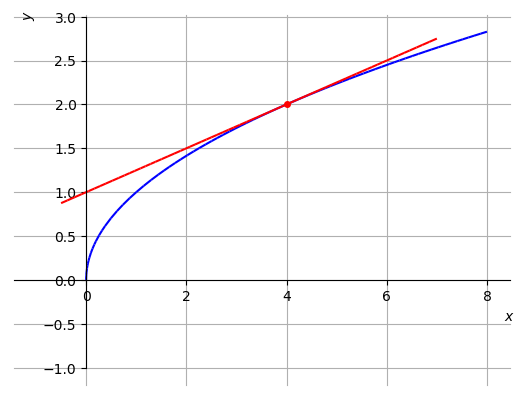
\includegraphics[width=0.7\textwidth]{./cap_deriv/dados/fig_cap_deriv_exeresol_rt_sqrt/fig_cap_deriv_exeresol_rt_sqrt}
    \caption{Esboços do gráfico da função $f$ e da reta tangente no ponto $x_0=4$.}
    \label{fig:cap_deriv_exeresol_rt_sqrt}
  \end{figure}
\end{resol}

\begin{exeresol}
  Considere que a produção em uma empresa tem custo
  \begin{equation}
    c(x) = \sqrt{x}
  \end{equation}
  e rendimento
  \begin{equation}
    r(x) = x^2,
  \end{equation}
  onde $x$ é o número de unidades (em milhões) produzidas. Calcule o lucro marginal da empresa quando $x=1$ mi.
\end{exeresol}
\begin{resol}
  O lucro é
  \begin{equation}
    l(x) = r(x) - c(x).
  \end{equation}
  Desta forma, o lucro marginal no ponto $x_0=1$ é
  \begin{align}
    l'(x_0) &= \lim_{h\to 0} \frac{l(x_0+h)-l(x_0)}{h}\\
            &= \lim_{h\to 0} \frac{r(x_0+h)-c(x_0+h)-(r(x_0)-c(x_0))}{h}\\
            &= \lim_{h\to 0} \frac{r(x_0+h)-r(x_0) - (c(x_0+h)-c(x_0))}{h}\\
            &= \lim_{h\to 0} \frac{r(x_0+h)-r(x_0)}{h} - \lim_{h\to 0} \frac{c(x_0+h)-c(x_0)}{h}\\
            &= r'(x_0) - c'(x_0)\\
            &= 2x_0 - \frac{1}{2\sqrt{x_0}}\\
            &= 2 - \frac{1}{2} = 1,5~\frac{\text{R\$}}{\text{un}}.
  \end{align}
\end{resol}


\subsection{Exercícios}

% \begin{flushright}
%   [Vídeo] | [Áudio] | \href{https://phkonzen.github.io/notas/contato.html}{[Contatar]}
% \end{flushright}

\begin{exer}
  Calcule as derivadas conforme indicado:
  \begin{enumerate}[a)]
  \item $f(x) = 2$, $f'(-1)$;
  \item $g(x) = 10^6$, $g'(10^8)$;
  \item $h(x) = \ln 2e$, $h'(-\pi)$;
  \end{enumerate}
\end{exer}
\begin{resp}
  a)~$0$; b)~$0$; c)~$0$
\end{resp}

\begin{exer}
  Calcule as derivadas conforme indicado:
  \begin{enumerate}[a)]
  \item $f(x) = 2 + x$, $f'(-1)$;
  \item $g(x) = 10^6 - 2x$, $g'(-3)$;
  \item $h(x) = \ln(2e) + ex$, $h'(10^6)$;
  \end{enumerate}  
\end{exer}
\begin{resp}
  a)~$-1$; b)~$-2$; c)~$e$
\end{resp}

\begin{exer}
  Calcule as derivadas conforme indicado:
  \begin{enumerate}[a)]
  \item $f(x) = x$, $f'(-1)$;
  \item $g(x) = -2x$, $g'(-3)$;
  \item $h(x) = ex$, $h'(10^6)$;
  \end{enumerate}  
\end{exer}
\begin{resp}
  a)~$-1$; b)~$-2$; c)~$e$
\end{resp}

\begin{exer}
  Determine a reta secante ao gráfico de $f(x) = 5-x^2$ pelos pontos $x_0=1$ e $x_1=2$. Então, determine a reta tangente ao gráfico de $f$ no ponto $x_0=1$. Por fim, faça os esboços dos gráficos de $f$, da reta secante e da reta tangente em um mesmo plano cartesiano.
\end{exer}
\begin{resp}
  reta secante: $y = -3x + 7$; reta tangente: $y = -2x + 6$; dica: verifique seus esboços plotando os gráficos no computador
\end{resp}

\begin{exer}
  Assumindo que, em uma empresa, a produção tenha o custo $c(x) = 2\sqrt{x}$ e rendimento $r(x) = \frac{1}{100}x^3$, dados em milhões de reais com $x$ em milhares de unidades. Calcule:
  \begin{enumerate}[a)]
  \item o custo marginal quando $x = 1$;
  \item o rendimento marginal quando $x = 1$;
  \item o lucro marginal quando $x=1$.
  \end{enumerate}
\end{exer}
\begin{resp}
  a)~$1000~\frac{\text{R}\$}{\text{un}}$; b)~$30~\frac{\text{R\$}}{\text{un}}$; c)~$-970~\frac{\text{R\$}}{\text{un}}$.
\end{resp}


\section{Função derivada}\label{cap_deriv_sec_funder}

\begin{flushright}
  [Vídeo] | [Áudio] | \href{https://phkonzen.github.io/notas/contato.html}{[Contatar]}
\end{flushright}

A {\bf derivada} de uma função $f$ em relação à variável $x$ é a função $\displaystyle f' = \frac{\dd f}{\dd x}$ cujo valor em $x$ é
\begin{equation}\label{eq:derivada}
  f'(x) = \lim_{h\to 0} \frac{f(x+h)-f(x)}{h},
\end{equation}
quando este limite existe. Dizemos que $f$ é {\bf derivável} (ou {\bf diferenciável}) em um ponto $x$ de seu domínio, quando o limite dado em \eqref{eq:derivada} existe. Se isso ocorre para todo número real $x$, dizemos que $f$ é derivável em toda parte.

\begin{ex}
  A derivada de $f(x) = x^2$ é
  \begin{align}
    f'(x) &= \lim_{h\to 0} \frac{f(x+h)-f(x)}{h}\\
          &= \lim_{h\to 0} \frac{(x+h)^2 - x^2}{h}\\
          &= \lim_{h\to 0} \frac{x^2+2xh+h^2-x^2}{h}\\
          &= \lim_{h\to 0} 2x+h = 2x.
  \end{align}
  Observamos que este é o caso de uma função derivável em toda parte.A Figura \ref{fig:deriv_ex_ffl_x2}.

  \begin{figure}[H]
    \centering
    \includegraphics[width=0.7\textwidth]{./cap_deriv/dados/fig_deriv_ex_ffl_x2/fig}
    \caption{Esboços dos gráficos da função $f(x)=x^2$ e de sua derivada $f'(x) = 2x$.}
    \label{fig:deriv_ex_ffl_x2}
  \end{figure}  
  
  \ifispython
  Com o \sympy, podemos usar os seguintes comandos para verificarmos este resultado:
  \begin{lstlisting}
    from sympy import *
    x,h = symbols('x,h')
    f = lambda x: x**2
    limit((f(x+h)-f(x))/h,h,0)
  \end{lstlisting}

  Mais adequadamente, podemos usar o comando:
  \begin{lstlisting}
    diff(x**2,x)
  \end{lstlisting}
  ou, equivalentemente,
  \begin{lstlisting}
    diff(x**2)
  \end{lstlisting}
  para computar a derivada de $x^2$ em relação a $x$.
  \fi
\end{ex}

\begin{obs}
  A derivada à direita (à esquerda) de uma função $f$ em um ponto $x$ é definida por
  \begin{equation}
    f_{\pm}'(x) = \frac{\dd f}{\dd x^{\pm}} = \lim_{h\to 0^\pm} \frac{f(x+h)-f(x)}{h}.
  \end{equation}
  Desta forma, no caso de pontos extremos do domínio de uma função, empregamos a derivada lateral correspondente.
\end{obs}

\begin{ex}\label{ex:deriv_sqrtx}
  Vamos calcular a derivada de $f(x) = \sqrt{x}$. Para $x=0$, só faz sentido calcular a derivada lateral à direta:
  \begin{align}
    f'_{+}(0) &= \lim_{h\to 0^+} \frac{\sqrt{0+h}-\sqrt{0}}{h} \\
              &= \lim_{h\to 0^+} \frac{\sqrt{h}}{h} \\
              &= \lim_{h\to 0^+} \frac{1}{\cancelto{0^+}{\sqrt{h}}} = +\infty.
  \end{align}
  Ou seja, $f(x) = \sqrt{x}$ não é derivável em $x=0$. Agora, para $x> 0$, temos
  \begin{align}
    f'(x) &= \lim_{h\to 0} \frac{\sqrt{x+h}-\sqrt{x}}{h}\\
          &= \lim_{h\to 0} \frac{\sqrt{x+h}-\sqrt{x}}{h}\cdot \frac{\sqrt{x+h}+\sqrt{x}}{\sqrt{x+h}+\sqrt{x}}\\
          &= \lim_{h\to 0} \frac{x+h-x}{h(\sqrt{x+h}+\sqrt{x})}\\
          &= \frac{1}{2\sqrt{x}}.
  \end{align}
  Na Figura \ref{fig:deriv_ex_ffl_sqrtx}, temos os esboços dos gráficos desta função e de sua derivada.

  \begin{figure}[H]
    \centering
    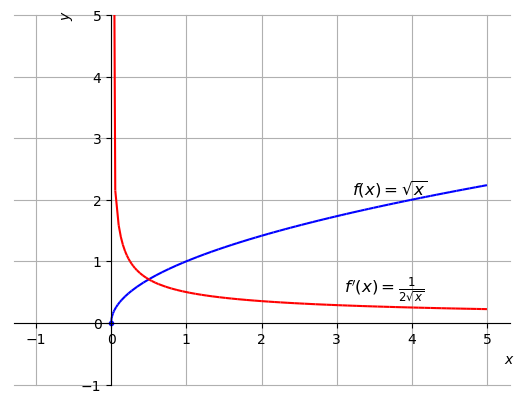
\includegraphics[width=0.7\textwidth]{./cap_deriv/dados/fig_deriv_ex_ffl_sqrtx/fig_deriv_ex_ffl_sqrtx}
    \caption{Esboços dos gráficos da função $f(x)=\sqrt{x}$ e de sua derivada.}
    \label{fig:deriv_ex_ffl_sqrtx}
  \end{figure}

  \ifispython
  No \sympy, a computação de $f'_{+}(0)$ pode ser feita com os comandos\footnote{Por padrão no \sympy, o limite é tomado à direita.}:
  \begin{lstlisting}
    from sympy import *
    h = Symbol('h')
    limit((sqrt(0+h)-sqrt(0))/h,h,0)
  \end{lstlisting}
  E, a derivada de $f(x) = \sqrt{x}$ (nos pontos de diferenciabilidade) pode ser obtida com o comando:
  \begin{lstlisting}
    diff(sqrt(x),x)
  \end{lstlisting}
  \fi
\end{ex}

\begin{ex}\label{ex:deriv_dabs}
  A função valor absoluto é derivável para todo $x\neq 0$ e não é derivável em $x=0$. De fato, para $x<0$ temos
  \begin{align}
    f'(x) &= \lim_{h\to 0} \frac{|x+h|-|x|}{h}\\
          &= \lim_{h\to 0} \frac{-(x+h)+x}{h}\\
          &= \lim_{h\to 0} \frac{h}{h} = 1.
  \end{align}
  Analogamente, para $x>0$ temos
  \begin{align}
    f'(x) &= \lim_{h\to 0} \frac{|x+h|-|x|}{h}\\
          &= \lim_{h\to 0} \frac{x+h-x}{h}\\
          &= \lim_{h\to 0} \frac{h}{h} = 1.
  \end{align}
  Agora, para $x=0$, devemos verificar as derivadas laterais:
  \begin{align}
    f'_+(0) &= \lim_{h\to 0^+} \frac{|h|-|0|}{h} = \lim_{h\to 0^+} \frac{h}{h} = 1,\\
    f'_-(0) &= \lim_{h\to 0^-} \frac{|h|-|0|}{h} = \lim_{h\to 0^-} \frac{-h}{h} = -1.
  \end{align}
  Como as derivadas laterais são diferentes, temos que $y = |x|$ não é derivável em $x=0$. Na figura \ref{fig:deriv_ex_ffl_absx}, temos os esboços dos gráficos de $f(x) = |x|$ e sua derivada
  \begin{equation}\label{eq:deriv_signx}
    f'(x) = \left\{
      \begin{array}[H]{rr}
        -1 &, x<0,\\
        1 &, x> 0
      \end{array}
    \right.
  \end{equation}
  Esta é chamada de {\bf função sinal} e denotada por $\sign(x)$. Ou seja, a função sinal é a derivada da função valor absoluto.

  \begin{figure}[H]
    \centering
    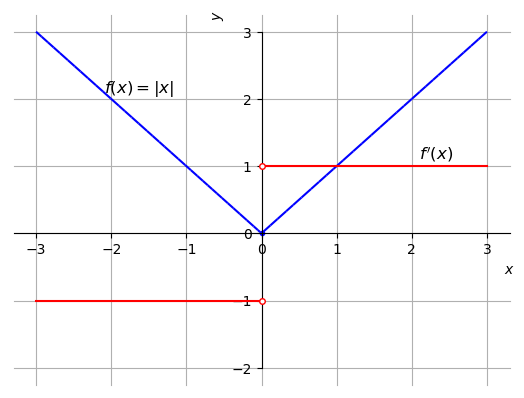
\includegraphics[width=0.7\textwidth]{./cap_deriv/dados/fig_deriv_ex_ffl_absx/fig_deriv_ex_ffl_absx}
    \caption{Esboços dos gráficos da função $f(x)=|x|$ e de sua derivada.}
    \label{fig:deriv_ex_ffl_absx}
  \end{figure}

  \ifispython
  No \sympy, podemos computar a derivada da função valor absoluto com o comando:
  \begin{lstlisting}
    In : from sympy import *
    ...: x = symbols('x', real=True)
    ...: diff(abs(x))
    Out: sign(x)
  \end{lstlisting}
  \fi
\end{ex}

\subsection{Continuidade de uma função derivável}

\begin{flushright}
  [Vídeo] | [Áudio] | \href{https://phkonzen.github.io/notas/contato.html}{[Contatar]}
\end{flushright}

Uma função $y=f(x)$ {\bf derivável} em $x=x_0$ é {\bf contínua} neste ponto. De fato, lembramos que $f$ é contínua em $x=x_0$ quando $x_0$ é um ponto de seu domínio e
\begin{equation}
  \lim_{x\to x_0} f(x) = f(x_0).
\end{equation}
Isto é equivalente a
\begin{equation}
  \lim_{h\to 0} f(x_0+h) = f(x_0)
\end{equation}
ou, ainda,
\begin{equation}
  \lim_{h\to 0} \left[f(x_0+h)-f(x_0)\right] = 0.
\end{equation}
Vamos mostrar que este é o caso quando $f$ é derivável em $x=x_0$. Neste caso, temos
\begin{align}
  \lim_{h\to 0} \left[f(x_0+h)-f(x_0)\right] &= \lim_{h\to 0} \left[f(x_0+h)-f(x_0)\right]\cdot \frac{h}{h} \\
                                             &= \lim_{h\to 0} \left[\cancelto{f'(x_0)}{\frac{f(x_0+h)-f(x_0)}{h}}\right]\cdot h \\
                                             &= \lim_{h\to 0} f'(x_0)\cdot h \\
                                             &= 0.
\end{align}
Ou seja, de fato, se $f$ é derivável em $x=x_0$, então $f$ é contínua em $x=x_0$.

\begin{obs}
  A recíproca não é verdadeira, uma função $f$ ser contínua em um ponto $x=x_0$ não garante que ela seja derivável em $x=x_0$. No Exemplo \ref{ex:deriv_dabs}, vimos que a função valor absoluto $f(x) = |x|$ não derivável em $x=0$, enquanto esta função é contínua (veja, também, o Exemplo \ref{ex:lim_fabs_cont}).
\end{obs}

\subsection{Derivadas de ordens mais altas}

\begin{flushright}
  [Vídeo] | [Áudio] | \href{https://phkonzen.github.io/notas/contato.html}{[Contatar]}
\end{flushright}

A derivada de uma função $y = f(x)$ em relação a $x$ é a função $y = f'(x)$. Quando esta é diferenciável, podemos calcular a derivada da derivada. Esta é conhecida como a {\bf segunda derivada} de $f$, denotamos
\begin{equation}
  f''(x) := (f'(x))' ~ \text{ou} ~ \frac{\dd^2}{\dd x^2}f(x) = \frac{\dd}{\dd x}\left(\frac{\dd}{\dd x}f(x)\right).
\end{equation}

\begin{ex}\label{ex:deriv_fll}
  Seja $f(x) = x^3$. Então, a primeira derivada de $f$ é
  \begin{align}
    f'(x) &= \lim_{h\to 0} \frac{f(x+h)-f(x)}{h} \\
          &= \lim_{h\to 0} \frac{(x+h)^3-x^3}{h}\\
          &= \lim_{h\to 0} \frac{x^3+3x^2h+3xh^2+h^3-x^3}{h}\\
          &= \lim_{h\to 0} 3x^2+\cancelto{0}{3xh}+\cancelto{0}{h^2} = 3x^2.
  \end{align}
  De posse da primeira derivada $f'(x) = 3x^2$, podemos calcular a segunda derivada de $f$, como segue:
  \begin{align}
    f''(x) &= [f'(x)]' \\
           &= \lim_{h\to 0} \frac{f'(x+h)-f'(x)}{h} \\
           &= \lim_{h\to 0} \frac{3(x+h)^2-3x^2}{h} \\
           &= \lim_{h\to 0} \frac{3x^2+6xh+h^2-3x^2}{h} \\
           &= \lim_{h\to 0} 6x+\cancelto{0}{h} = 6x,
  \end{align}
  i.e. $f''(x) = 6x$.

  \ifispython
  No \sympy, podemos computar a segunda derivada da função com o comando:
  \begin{lstlisting}
    In : from sympy import *
    ...: x = symbols('x')
    ...: diff(x**3,x,2)
    Out: 6*x
  \end{lstlisting}
  \fi  
\end{ex}

Generalizando, quando existe, a $n$-ésima derivada de uma função $y = f(x)$, $n\geq 1$, é recursivamente definida (e denotada) por
\begin{equation}
  f^{(n)}(x) := [f^{(n-1)}]' ~ \text{ou} ~ \frac{\dd^n}{\dd x^n}f(x) := \frac{\dd}{\dd x}\left[\frac{\dd^{n-1}}{\dd x^{n-1}}f(x)\right],
\end{equation}
com $f^{(3)}\equiv f'''$, $f^{(2)}\equiv f''$, $f^{(1)}\equiv f'$ e $f^{(0)}\equiv f$.

\begin{ex}
  A terceira derivada de $f(x) = x^3$ em relação a $x$ é $f'''(x) = [f''(x)]'$. No exemplo anterior (Exemplo \ref{ex:deriv_fll}), calculamos $f''(x) = 6x$. Logo,
    \begin{align}
      f'''(x) &= [6x]' \\
              &= \lim_{h\to 0} \frac{6(x+h)-6x}{h} \\
              &= \lim_{h\to 0} 6 = 6.
    \end{align}

    A quarta derivada de $f(x) = x^3$ em relação a $x$ é $f^{(4)}(x) \equiv 0$, bem como $f^{(5)}(x) \equiv 0$. Verifique!

    \ifispython
    No \sympy, podemos computar a terceira derivada da função com o comando:
    \begin{lstlisting}
      In : from sympy import *
      ...: x = symbols('x')
      ...: diff(x**3,x,3)
      Out: 6
    \end{lstlisting}
  \fi  
\end{ex}


\subsection{Exercícios resolvidos}

% \begin{flushright}
%   [Vídeo] | [Áudio] | \href{https://phkonzen.github.io/notas/contato.html}{[Contatar]}
% \end{flushright}

\begin{exeresol}
  Calcule a derivada da função $f(x) = x^2 + 2x + 1$ em relação a $x$.
\end{exeresol}
\begin{resol}
  Por definição da derivada, temos
  \begin{align}
    f'(x) &= \lim_{h\to 0} \frac{f(x+h)-f(x)}{h}\\
          &= \lim_{h\to 0} \frac{(x+h)^2 + 2(x+h) + 1 - (x^2+2x+1)}{h}\\
          &= \lim_{h\to 0} \frac{x^2+2xh+h^2+2x+2h+1-x^2-2x-1}{h}\\
          &= \lim_{h\to 0} \frac{2xh+h^2+2h}{h}\\
          &= \lim_{h\to 0} 2x+h+2 = 2x+2.
  \end{align}
\end{resol}

\begin{exeresol}
  Determine os pontos de diferenciabilidade da função $f(x) = |x-1|$.
\end{exeresol}
\begin{resol}
  O gráfico da função $f(x) = |x-1|$ tem um bico no ponto $x=1$ (verifique!). Para valores de $x<1$, temos
  \begin{align}
    f'(x) &= \lim_{h\to 0} \frac{f(x+h) - f(x)}{h}\\
          &= \lim_{h\to 0} \frac{|\overbrace{x+h-1}^{<0}| - |\overbrace{x-1}^{<0}|}{h}\\
          &= \lim_{h\to 0} \frac{-x-h+1+x-1}{h}\\
          &= \lim_{h\to 0} \frac{-h}{h} = -1.
  \end{align}
  Para valores de $x > 1$, temos
  \begin{align}
    f'(x) &= \lim_{h\to 0} \frac{f(x+h) - f(x)}{h}\\
          &= \lim_{h\to 0} \frac{|\overbrace{x+h-1}^{>0}| - |\overbrace{x-1}^{>0}|}{h}\\
          &= \lim_{h\to 0} \frac{x+h-1-x+1}{h}\\
          &= \lim_{h\to 0} \frac{h}{h} = 1.
  \end{align}
  Ou seja, temos que $f(x) = |x-1|$ é diferenciável para $x\neq 1$. Agora, para $x=1$, temos
  \begin{align}
    f'_{-}(x) &= \lim_{h\to 0^{-}} \frac{f(1+h) - f(1)}{h}\\
              &= \lim_{h\to 0^{-}} \frac{|\overbrace{h}^{<0}| - |1-1|}{h}\\
              &= \lim_{h\to 0^{-}} \frac{-h}{h} = -1\\
    f'_{+}(x) &= \lim_{h\to 0^{+}} \frac{f(1+h) - f(1)}{h}\\
          &= \lim_{h\to 0^{+}} \frac{|\overbrace{h}^{>0}| - |1-1|}{h}\\
              &= \lim_{h\to 0^{+}} \frac{h}{h} = 1\\
  \end{align}
  Como $f'_{-}(1)\neq f'_{+}(1)$, temos que $\nexists f'(1)$. Concluímos que $f(x) = |x-1|$ é diferenciável nos pontos $\mathbb{R}\setminus\{1\}$. 
\end{resol}

\begin{exeresol}
  Calcule a segunda derivada em relação a $x$ da função
  \begin{equation}
    f(x) = x - x^2.
  \end{equation}
\end{exeresol}
\begin{resol}
  Começamos calculando a primeira derivada da função:
  \begin{align}
    f'(x) &= \lim_{h\to 0} \frac{f(x+h)-f(x)}{h} \\
          &= \lim_{h\to 0} \frac{(x+h)-(x+h)^2-(x-x^2)}{h} \\
          &= \lim_{h\to 0} \frac{x+h-x^2-2xh-h^2-x+x^2}{h} \\
          &= \lim_{h\to 0} 1-2x-\cancelto{0}{h} = 1 - 2x.
  \end{align}
  Então, calculamos a segunda derivada como segue
  \begin{align}
    f''(x) &= [f'(x)]' \\
           &= \lim_{h\to 0} \frac{f'(x+h)-f'(x)}{h} \\
           &= \lim_{h\to 0} \frac{1-2(x+h)-(1-2x)}{h} \\
           &= \lim_{h\to 0} -2 = -2.
  \end{align}
\end{resol}

\subsection{Exercícios}

% \begin{flushright}
%   [Vídeo] | [Áudio] | \href{https://phkonzen.github.io/notas/contato.html}{[Contatar]}
% \end{flushright}

\begin{exer}
  Calcule a derivada em relação a $x$ de cada uma das seguintes funções:
  \begin{enumerate}[a)]
  \item $f(x) = 2$
  \item $g(x) = -3$
  \item $h(x) = \sqrt{e}$
  \end{enumerate}
\end{exer}
\begin{resp}
  a)~$0$; b)~$0$; c)~$0$
\end{resp}

\begin{exer}
  Calcule a derivada em relação a $x$ de cada uma das seguintes funções:
  \begin{enumerate}[a)]
  \item $f(x) = 2x$
  \item $g(x) = -3x$
  \item $h(x) = \sqrt{e}x$
  \end{enumerate}
\end{exer}
\begin{resp}
  a)~$2$; b)~$-3$; c)~$\sqrt{e}$
\end{resp}

\begin{exer}
  Calcule a derivada em relação a $x$ da função
  \begin{equation}
    f(x) = x^2 - 2x + 1.
  \end{equation}
\end{exer}
\begin{resp}
  $f'(x) = 2x - 2$
\end{resp}

\begin{exer}
  Determine os pontos de diferenciabilidade da função $f(x) = \sqrt{x-1}$.
\end{exer}
\begin{resp}
  $(1, \infty)$
\end{resp}

\begin{exer}
  Considerando
  \begin{equation}
    f(x) = x^2-x^3,
  \end{equation}
  calcule:
  \begin{enumerate}[a)]
  \item $f'(x)$
  \item $f''(x)$
  \item $f'''(x)$
  \item $f^{(4)}$
  \item $f^{(1001)}(x)$
  \end{enumerate}
\end{exer}
\begin{resp}
  a)~$2x-3x^2$; b)~$2-6x$; c)~$-6$; d)~$0$; e)~$0$
\end{resp}

\section{Derivada de Funções Constante, Identidade e Potência}\label{cap_deriv_sec_funcip}

\begin{flushright}
  [YouTube] | [Vídeo] | [Áudio] | \href{https://phkonzen.github.io/notas/contato.html}{[Contatar]}
\end{flushright}

Nesta seção, vamos estudar as derivadas de função constante, de função identidade e de função potência.

\subsection{Derivada de Função Constante}

\begin{flushright}
  [YouTube] | [Vídeo] | [Áudio] | \href{https://phkonzen.github.io/notas/contato.html}{[Contatar]}
\end{flushright}

A derivada de função constante $f(x) \equiv k$, com $k$ constante, é
\begin{equation}
  {\color{blue}(k)' = 0}
\end{equation}
De fato, da definição de derivada temos
\begin{align}
  f'(x) &= \lim_{h\to 0} \frac{f(x+h)-f(x)}{h}\\
        &= \lim_{h\to 0} \frac{k-k}{h} \\
        &= \lim_{h\to 0} 0 = 0.
\end{align}

\begin{ex}
  Estudemos os seguintes casos:
  \begin{enumerate}[a)]
  \item $(2)' = 0$
  \item $(-3)' = 0$
  \item $(\pi)' = 0$
  \item $(a)' = 0$ para qualquer $a\in\mathbb{R}$
  \end{enumerate}
  \ifispython
  Com {\python}+{\sympy}, podemos computar essas derivadas com os seguintes comandos:
  \begin{lstlisting}
    In : from sympy import *
    In : diff(2)
    Out: 0
    
    In : diff(-3)
    Out: 0

    In : diff(pi)
    Out: 0

    In : x = Symbol('x')
    In : a = Symbol('a', const=True)
    In : diff(a, x)
    Out: 0
  \end{lstlisting}
  \fi
\end{ex}

\subsection{Derivada de Função Identidade}

\begin{flushright}
  [YouTube] | [Vídeo] | [Áudio] | \href{https://phkonzen.github.io/notas/contato.html}{[Contatar]}
\end{flushright}

A derivada da função identidade $f(x) = x$ é
\begin{equation}
  {\color{blue}(x)' = 1}
\end{equation}
De fato, da definição de derivada temos
\begin{align}
  f'(x) &= \lim_{h\to 0} \frac{f(x+h)-f(x)}{h}\\
        &= \lim_{h\to 0} \frac{x+h-x}{h}\\
        &= \lim_{h\to 0} \frac{h}{h} = 1.\\
\end{align}

\ifispython
\begin{ex}
  Usando {\python}+{sympy}, podemos computar a derivada da função identidade com as seguintes instruções:
  \begin{lstlisting}
    In : from sympy import *
    In : x = Symbol('x')
    In : diff(x)
    Out: 1
  \end{lstlisting}
\end{ex}
\fi

\subsection{Derivada de Função Potência}\label{cap_deriv_sec_funcip:ssec:funpot}

\begin{flushright}
  [YouTube] | [Vídeo] | [Áudio] | \href{https://phkonzen.github.io/notas/contato.html}{[Contatar]}
\end{flushright}

A derivada da função potência $f(x) = x^n$, $n$ número inteiro positivo, é
\begin{equation}
  {\color{blue}\left(x^n\right)' = nx^{n-1}}
\end{equation}
De fato, da definição de derivada, temos
\begin{align}
  f'(x) &= \lim_{h\to 0} \frac{f(x+h)-f(x)}{h}\\
        &= \lim_{h\to 0} \frac{(x+h)^n-x^n}{h}
\end{align}
Usando binômio de Newton\footnote{Isaac Newton, 1643 - 1727, matemático inglês. Fonte: \href{https://pt.wikipedia.org/wiki/Isaac_Newton}{Wikipédia}.}, temos
\begin{align}
  (x+h)^n &= \sum_{k=0}^n \binom{n}{k}x^{n-k}h^k,
\end{align}
onde os coeficientes binomiais são
\begin{equation}
  \binom{n}{k} = \frac{n!}{k!(n-k)!}.
\end{equation}
Assim, segue que
\begin{align}
  f'(x) &= \lim_{h\to 0} \frac{x^n+nx^{n-1}h+\frac{n(n-1)}{2}x^{n-2}h^2 + \cdots +h^n-x^n}{h}\\
        &= \lim_{h\to 0} nx^{n-1}+\frac{n(n-1)}{2}x^{n-2}h+\cdots+h^{n-1}\\
        &= nx^{n-1}.
\end{align}

\begin{ex}
  Estudemos os seguintes casos:
  \begin{enumerate}[a)]
  \item $\left(x^2\right)' = 2x^{1-1} = 2x$
  \item $\left(x^5\right)' = 5x^{5-1} = 5x^4$
  \item $\left(x^{2001}\right)' = 2001x^{2000}$
  \item $\left(x^m\right)' = mx^{m-1}$ para qualquer $m$ inteiro positivo.
  \end{enumerate}
  \ifispython
  Com {\python}+{\sympy}, podemos computar essas derivadas com os seguintes comandos:
  \begin{lstlisting}
    In : from sympy import *
    In : x = Symbol('x')
    In : diff(x**2)
    Out: 2*x

    In : diff(x**5)
    Out: 5*x**4

    In : diff(x**2001)
    Out: 2001*x**2000

    In : m = Symbol('m', integer=True, positive=True)
    In : simplify(diff(x**m, x))
    Out: m*x**(m - 1)
  \end{lstlisting}
  \fi
\end{ex}

\begin{obs}
  Ao longo das notas de Cálculo, vamos estudar que a fórmula de derivação
  \begin{equation}
    {\color{blue}(x^r)'= rx^{r-1}}
  \end{equation}
  {\bf vale para qualquer $r$ número real não nulo}, considerando-se o domínio natural das funções potência. Assim sendo, vamos assumir passar a aplicá-la para qualquer função potência a partir de agora.
\end{obs}

\begin{ex}
  Estudemos os seguintes casos:
  \begin{enumerate}[a)]
  \item $\displaystyle\left(x^{-1}\right)' = -1x^{-1-1} = -x^{-2}$
  \item $\displaystyle\left(x^{\frac{1}{2}}\right)' = \frac{1}{2}x^{\frac{1}{2}-1} = \frac{1}{2}x^{-\frac{1}{2}}$
  \item $\displaystyle\left(x^e\right)' = ex^{e-1}$
  \end{enumerate}
  \ifispython
  Com {\python}+{\sympy}, podemos computar essas derivadas com os seguintes comandos:
  \begin{lstlisting}
    In : from sympy import *
    In : x = Symbol('x')
    In : diff(x**(-1))
    Out: -1/x**2

    In : diff(x**(S(1)/2))
    Out: 1/(2*sqrt(x))

    In : diff(x**E)
    Out: E*x**E/x
  \end{lstlisting}
  \fi  
\end{ex}

\subsection{Lista de derivadas}

\begin{align}
  &(k)' = 0\\
  &(x)' = 1\\
  &(x^n)' = nx^{n-1}
\end{align}


\subsection{Exercícios Resolvidos}

\begin{exeresol}
  Calcule o ângulo de declividade da reta tangente ao gráfico de cada uma das seguintes funções em qualquer ponto fixado $x = x_0$.
  \begin{enumerate}[a)]
  \item Função constante $f(x) \equiv k$
  \item Função identidade $f(x) = x$
  \end{enumerate}
\end{exeresol}
\begin{resol}
  O ângulo $\theta$ de declividade da reta tangente ao gráfico de uma dada função $f$ em um ponto $x=x_0$ é
  \begin{equation}
    \theta = \arctg(f'(x_0)).
  \end{equation}
  \begin{enumerate}[a)]
  \item Função constante $f(x) \equiv k$

    Nesse caso, $f'(x) = 0$ para todo $x$, logo
    \begin{align*}
      \theta &= \arctg(0)\\
             &= 0.
    \end{align*}
  \item Função identidade $f(x) = x$

    Nesse caso, $f'(x) = 1$ para todo $x$, logo
    \begin{align*}
      \theta &= \arctg(1)\\
             &= \frac{\pi}{4}
    \end{align*}
  \end{enumerate}
\end{resol}

\begin{exeresol}
  Determine a equação da reta tangente ao gráfico da função $f(x) = x^2$ no ponto $x=1$.
\end{exeresol}
\begin{resol}
  A equação da reta tangente ao gráfico de uma função $f$ em um ponto $x = x_0$ é
  \begin{equation}
    y = f'(x_0)(x-x_0) + f(x_0)
  \end{equation}
  Nesse caso,
  \begin{equation}
    y = f'(1)(x-1) + f(1)
  \end{equation}
  Temos $f(1) = (1)^2 = 1$. Agora, pela derivada de função potência, temos
  \begin{equation}
    f'(x) = (x^2)' = 2x
  \end{equation}
  Logo,
  \begin{equation}
    f'(1) = 2\cdot 1 = 2
  \end{equation}
  Concluímos que equação da reta tangente é
  \begin{gather}
    y = 2(x-1) + 1\\
    y = 2x - 1
  \end{gather}
\end{resol}

\subsection{Exercícios}

\begin{exer}
  Calcule as seguintes derivadas:
  \begin{enumerate}[a)]
  \item $(7)'$
  \item $(-1,7)'$
  \item $\left(\sqrt{2}\right)'$
  \item $\left(\sec(\pi)\right)'$
  \end{enumerate}
\end{exer}
\begin{resp}
  a) $0$; b) $0$; c) $0$; d) $0$
\end{resp}

\begin{exer}
  Calcule as seguintes derivadas:
  \begin{enumerate}[a)]
  \item $\left(x\right)'$
  \item $\left(x^3\right)'$
  \item $\left(\sqrt{x}\right)'$
  \item $\displaystyle\left(\frac{1}{x}\right)'$
  \item $\displaystyle\left(\frac{1}{\sqrt[3]{x^2}}\right)'$
  \item $\left(x^\pi\right)'$
  \end{enumerate}
\end{exer}
\begin{resp}
  a) $1$; b) $3x^2$; c) $\displaystyle\frac{1}{2\sqrt{x}}$; d) $\displaystyle -\frac{1}{x^2}$; e) $\displaystyle -\frac{2}{3\sqrt[3]{x^5}}$; f) $\pi x^{\pi - 1}$
\end{resp}

\begin{exer}
  Calcule as seguintes derivadas de ordem mais alta:
  \begin{enumerate}[a)]
  \item $(2)''$
  \item $\left(2^{1001}\right)'''$
  \item $\left[(-3)^{4}\right]^{(4)}$
  \end{enumerate}
\end{exer}
\begin{resp}
  a) $0$; b) $0$; c) $0$
\end{resp}

\begin{exer}
  Calcule o coeficiente angular da reta tangente $y = mx + b$ ao gráfico da função $f(x) = x^3$ no ponto $x = 0$. Faça o esboço do gráfico desta função.
\end{exer}
\begin{resp}
  $0$
\end{resp}

\begin{exer}
  Calcule o ponto de interseção das retas tangentes ao gráfico da função $f(x) = x^2$ nos pontos $x_0=-1$ e $x_1 = 1$. Faça, em um mesmo esboço, os gráficos de $f$ e das retas tangentes calculadas.
\end{exer}
\begin{resp}
  $(0, -1)$
\end{resp}

\section{Derivada de Funções Exponenciais e Logarítmicas}\label{cap_deriv_sec_funexplog}

\begin{flushright}
  [YouTube] | [Vídeo] | [Áudio] | \href{https://phkonzen.github.io/notas/contato.html}{[Contatar]}
\end{flushright}

Nesta seção vamos estudar a derivada de funções exponenciais e logarítmicas. Começamos com a definição no número de Euler\footnote{Leonhard Paul Euler, 1707 - 1783, matemático suíço. Fonte: \href{https://pt.wikipedia.org/wiki/Leonhard_Euler}{Wikipédia}.} por limites.

\subsection{Número de Euler}

\begin{flushright}
  [YouTube] | [Vídeo] | [Áudio] | \href{https://phkonzen.github.io/notas/contato.html}{[Contatar]}
\end{flushright}

O número de Euler $e\approx 2,7183...$ pode ser definido pelo seguinte limite
\begin{equation}\label{eq:defe}
  {\color{blue} e = \lim_{h\to 0}(1 + h)^{\frac{1}{h}}}
\end{equation}

\begin{ex}
  Consideremos os seguintes limites.
  \begin{enumerate}[a)]
  \item $\displaystyle\lim_{h\to 0} (1 + h)^{\frac{2}{h}}$
    \begin{align}
      \lim_{h\to 0} (1 + h)^{\frac{2}{h}} &= \lim_{h\to 0} \left[(1 + h)^{\frac{1}{h}}\right]^2\\
                                                     &= \left[\lim_{h\to 0}\cancelto{e}{(1 + h)^{\frac{1}{h}}}\quad\right]^2\\
                                                     &= e^2
    \end{align}
    \ifispython
    Com o {\python}+{\sympy}, podemos computar este limite com os seguintes comandos:
    \begin{lstlisting}
      In : from sympy import *
      ...: h = Symbol('h')
      ...: limit((1+h)**(2/h), h, 0)
      Out: exp(2)
    \end{lstlisting}
    \fi
  \item $\displaystyle \lim_{h\to 0}\left(1 + 2h\right)^{\frac{1}{h}}$
    
    Para calcular este limite, podemos fazer a seguinte \emph{mudança de variável}
    \begin{equation}
      u = 2h
    \end{equation}
    donde, temos que $u\to 0$ quando $h\to 0$. Então, segue que
    \begin{align}
      \lim_{h\to 0}\left(1 + 2h\right)^{\frac{1}{h}} &= \lim_{u\to 0}\left(1 + u\right)^{\frac{2}{u}}\\
                                                     &= e^2
    \end{align}
    \ifispython
    Com o {\python}+{\sympy}, podemos computar este limite com os seguintes comandos:
    \begin{lstlisting}
      In : from sympy import *
      ...: h = Symbol('h')
      ...: limit((1+2*h)**(1/h), h, 0)
      Out: exp(2)
    \end{lstlisting}
    \fi
  \end{enumerate}
\end{ex}

\subsection{Derivada de Funções Exponenciais}\label{cap_deriv_sec_funexplog:ssec:dexp}

\begin{flushright}
  [YouTube] | [Vídeo] | [Áudio] | \href{https://phkonzen.github.io/notas/contato.html}{[Contatar]}
\end{flushright}

Vamos calcular a derivada da função exponencial
\begin{equation}
  f(x) = a^x
\end{equation}
com $a>0$. Partindo da definição de definição de derivada, temos
\begin{align}
  f'(x) &= \lim_{h\to 0}\frac{f(x+h)-f(x)}{h}\\
        &= \lim_{h\to 0}\frac{a^{x+h}-a^x}{h}\\
        &= \lim_{h\to 0}\frac{a^x\left(a^h-1\right)}{h}\\
        &= a^x\lim_{h\to 0}\frac{a^h-1}{h}\label{eq:ax_aux}
\end{align}
Agora, fazemos a seguinte \emph{mudança de variável}
\begin{equation}
  u = a^h-1
\end{equation}
donde, $u\to 0$ quando $h\to 0$ e
\begin{equation}
  h = \log_a(1 + u).
\end{equation}
Com isso, voltando a \eqref{eq:ax_aux} segue que
\begin{align}
  \left(a^x\right) &= a^x\lim_{u\to 0}\frac{u}{\log_a(1+u)}\\
                   &= a^x\lim_{u\to 0}\frac{1}{\frac{1}{u}\log_a(1+u)}\\
                   &= a^x\lim_{u\to 0}\frac{1}{\log_a\cancelto{e}{(1+u)^{\frac{1}{u}}}}\\
                   &= a^x\frac{1}{\log_a e}
\end{align}
Lembrando que
\begin{equation}
  \log_a x = \frac{\ln x}{\ln a}
\end{equation}
concluímos que
\begin{equation}
  {\color{blue}\left(a^x\right)' = a^x\ln a}
\end{equation}

No caso particular da \emph{função exponencial natural}, temos
\begin{equation}
  \left(e^x\right)' = e^x\ln e
\end{equation}
ou seja,
\begin{equation}
  {\color{blue}\left(e^x\right)' = e^x}
\end{equation}

\begin{ex}
  Estudemos os seguintes casos:
  \begin{enumerate}[a)]
  \item
    \begin{equation}
      \displaystyle\left(2^x\right)' = 2^x\ln 2
    \end{equation}
  \item
    \begin{equation}
      \displaystyle\left[\left(\frac{3}{2}\right)^x\right]' = \left(\frac{3}{2}\right)^x\ln\frac{3}{2}
    \end{equation}
  \item
    \begin{align}
      \displaystyle\left(e^{\frac{1}{2}x}\right)' &= \left[(\sqrt{e})^x\right]' \\
                                                  &= (\sqrt{e})^x\ln \sqrt{e}\\
                                                  &= \frac{1}{2}e^{\frac{1}{2}x}
    \end{align}
  \end{enumerate}
  \ifispython
  Com o {\python}+{\sympy}, podemos computar essas derivadas como segue:
  \begin{lstlisting}
    In : from sympy import *
    In : x = Symbol('x')
    In : diff(2**x)
    Out: 2**x*log(2)

    In : diff((S(3)/2)**x)
    Out: (3/2)**x*log(3/2)

    In : diff(exp(x/2))
    Out: exp(x/2)/2
  \end{lstlisting}
  \fi
\end{ex}

\subsection{Derivada de Funções Logarítmicas}\label{cap_deriv_sec_funexplog:ssec:dlog}

\begin{flushright}
  [YouTube] | [Vídeo] | [Áudio] | \href{https://phkonzen.github.io/notas/contato.html}{[Contatar]}
\end{flushright}

Vamos calcular a derivada da função logarítmica
\begin{equation}
  f(x) = \log_a x
\end{equation}
com $a>0$ e $a\neq 1$. Partimos da definição de derivada
\begin{align}
  f'(x) &= \lim_{h\to 0}\frac{f(x+h)-f(x)}{h}\\
        &= \lim_{h\to 0}\frac{\log_a(x+h)-\log_ax)}{h}\\
        &= \lim_{h\to 0}\frac{1}{h}\log_a\frac{x+h}{x}\\
        &= \lim_{h\to 0}\frac{1}{h}\log_a\left(1 + \frac{h}{x}\right)\\
        &= \lim_{h\to 0}\log_a\left(1 + \frac{h}{x}\right)^{\frac{1}{h}}
\end{align}
Tendo em vista que\footnote{Consulte o Exercício \ref{exer:cap_deriv_defe1ox}}
\begin{equation}
  e^{\frac{1}{x}} = \lim_{h\to 0}\left(1 + \frac{h}{x}\right)^{\frac{1}{h}}
\end{equation}
obtemos
\begin{align}
  (\log_a x)' &= \log_a e^{\frac{1}{x}}\\
              &= \frac{1}{x}\log_a e\\
              &= \frac{1}{x}\frac{\ln e}{\ln a}
\end{align}
e concluímos que
\begin{equation}
  {\color{blue}(\log_a x)' = \frac{1}{x\ln a}}
\end{equation}

Observamos que no caso particular da função logaritmo natural, segue que
\begin{equation}
  {\color{blue}(\ln x)' = \frac{1}{x}}
\end{equation}

\begin{ex}
  Estudemos os seguintes casos:
  \begin{enumerate}[a)]
  \item
    \begin{equation}
      (\log_2 x)' = \frac{1}{x\ln 2}
    \end{equation}
  \item
    \begin{equation}
      \left(\log_{\frac{3}{2}}x\right)' = \frac{1}{x\ln \frac{3}{2}}
    \end{equation}
  \item
    \begin{equation}
      (\ln x)' = \frac{1}{x}
    \end{equation}
  \end{enumerate}
\end{ex}

\subsection{Lista de derivadas}

\begin{align}
  &(k)' = 0\\
  &(x)' = 1\\
  &(x^n)' = nx^{n-1}\\
  &(a^x)' = a^x\ln a\\
  &(e^x)' = e^x\\
  &(\log_a x)' = \frac{1}{x\ln a}\\
  &(\ln x)' = \frac{1}{x}
\end{align}


\subsection{Exercícios Resolvidos}

\begin{exeresol}
  Mostre que
  \begin{equation}
    e = \lim_{h\to\infty} \left(1 + \frac{1}{h}\right)^h
  \end{equation}
\end{exeresol}
\begin{resol}
  Tendo em mente a definição dada na Equação \ref{eq:defe}, fazemos a seguinte mudança de variável
  \begin{equation}
    u = \frac{1}{h}
  \end{equation}
  donde, $u\to 0$ quando $h\to \infty$. Logo, temos
  \begin{align}
    \lim_{h\to\infty} \left(1 + \frac{1}{h}\right)^h &= \lim_{u\to 0} \left(1 + u\right)^{\frac{1}{u}}\\
                                                     &= e.
  \end{align}
\end{resol}

\begin{exeresol}
  Determine a equação da reta tangente ao gráfico de $y = \ln x$ no ponto $x=1$.
\end{exeresol}
\begin{resol}
  A equação da reta tangente ao gráfico de uma função $y = f(x)$ no ponto $x=x_0$ é
  \begin{equation}
    y = f'(x_0)(x-x_0) + f(x_0).
  \end{equation}
  Neste exercício, temos $x_0=1$ e $f(x) =\ln x$. Então, calculamos
  \begin{align}
    f'(x) &= (\ln x)'\\
          &= \frac{1}{x}
  \end{align}
  No ponto $x_0 = 1$, temos $f'(x_0) = 1/x_0 = 1$. Logo, a equação da reta tangente é
  \begin{gather}
    y = 1\cdot(x - 1) + f(1)
    y = x - 1 + 0\\
    y = x - 1
  \end{gather}
\end{resol}

\subsection{Exercícios}

\begin{exer}
  Calcule:
  \begin{enumerate}[a)]
  \item $\displaystyle \left(3^x\right)'$
  \item $\displaystyle \left[\left(\frac{2}{5}\right)^x\right]'$
  \end{enumerate}
\end{exer}
\begin{resp}
  a) $3^x\ln 3$; b) $\left(\frac{2}{5}\right)^x = \left(\frac{2}{5}\right)^x\ln\frac{2}{5}$
\end{resp}

\begin{exer}
  Calcule:
  \begin{enumerate}[a)]
  \item $\displaystyle \left(\frac{2^x}{5^x}\right)'$\\
  \item $\displaystyle \left(e^{2x}\right)'$
  \end{enumerate}
\end{exer}
\begin{resp}
  a) $\left(\frac{2}{5}\right)^x = \left(\frac{2}{5}\right)^x\ln\frac{2}{5}$; b) $2e^{2x}$
\end{resp}

\begin{exer}
  Calcule:
  \begin{enumerate}
  \item $\displaystyle\left(\log_3 x\right)'$
  \item $\displaystyle\left(\log_{\frac{2}{5}} x\right)'$
  \item $\displaystyle (\ln x)'$
  \end{enumerate}
\end{exer}
\begin{resp}
  a) $\displaystyle \frac{1}{x\ln 3}$ b) $\displaystyle\frac{1}{x\ln \frac{2}{5}}$; c) $\frac{1}{x}$
\end{resp}

\begin{exer}
  Encontre a equação da reta tangente ao gráfico de $f(x) = \ln x$ no ponto $x=1$.
\end{exer}
\begin{resp}
  $y = x-1$
\end{resp}

\begin{exer}\label{exer:cap_deriv_ex}
  Mostre que
  \begin{equation}
    e^x = \lim_{h\to 0}\left(1 + xh\right)^{\frac{1}{h}}
  \end{equation}
\end{exer}
\begin{resp}
  Dica! Consulte o Exemplo \ref{ex:nume_b}
\end{resp}

\begin{exer}\label{exer:cap_deriv_defe1ox}
  Mostre que
  \begin{equation}
    e^{\frac{1}{x}} = \lim_{h\to 0}\left(1 + \frac{h}{x}\right)^{\frac{1}{h}}
  \end{equation}
\end{exer}
\begin{resp}
  Dica! Consulte o Exercício \ref{exer:cap_deriv_ex}
\end{resp}

%ESTOU AQUI
\section{Regas Básicas de Derivação}\label{cap_deriv_sec_regrasderiv}

\begin{flushright}
  [YouTube] | [Vídeo] | [Áudio] | \href{https://phkonzen.github.io/notas/contato.html}{[Contatar]}
\end{flushright}

\subsection{Regras da multiplicação por constante e da soma}\label{cap_deriv_sec_regrasderiv:ssec:deriv_rmcs}

\begin{flushright}
  [Vídeo] | [Áudio] | \href{https://phkonzen.github.io/notas/contato.html}{[Contatar]}
\end{flushright}

Sejam $k$ um número real, $u = u(x)$ e $v = v(x)$ funções deriváveis. Temos as seguintes regras básicas de derivação:
\begin{itemize}
\item $\pmb{(k\cdot u)' = k\cdot u'}$.

  De fato, pela definição da derivada temos
  \begin{align}
    (k\cdot u)'(x) &= \lim_{h\to 0} \frac{k\cdot u(x+h)-k\cdot u(x)}{h} \\
                   &= \lim_{h\to 0} k\cdot \left(\frac{u(x+h)-u(x)}{h}\right) \\
                   &= k\cdot \lim_{h\to 0} \cancelto{u'}{\frac{u(x+h)-u(x)}{h}} \\
                   &= k\cdot u'.
  \end{align}
  
  \ifispython
  No \sympy, podemos usar os seguintes comandos para obtermos esta regra de derivação:
  \begin{lstlisting}
    from sympy import *
    k = Symbol('k', real=True)
    u = Function('u', real=True)
    diff(k*u(x),x)
  \end{lstlisting}
  \fi

\item $\pmb{(u\pm v)' = u'\pm v'}$.

  De fato, temos
  \begin{align}
    (u + v)'(x) &= \lim_{h\to 0} \frac{(u + v)(x+h)-(u + v)(x)}{h}\\
                &= \lim_{h\to 0} \frac{u(x+h)+v(x+h)-[u(x)+v(x)]}{h}\\
                &= \lim_{h\to 0} \left[\cancelto{u'}{\frac{u(x+h)-u(x)}{h}} \right. \\
                &+ \left. \cancelto{v'}{\frac{v(x+h)-v(x)}{h}}\right]\\
                &= u'(x) + v'(x).
  \end{align}

  Também, como $(-v)' = (-1\cdot v)' = -1\cdot v' = -v'$, temos
  \begin{equation}
    (u-v)' = [u+(-v)]' = u' + (-v)' = u' - v'.
  \end{equation}
  
  \ifispython
  No \sympy, podemos usar os seguintes comandos para obtermos a regra de derivação para soma:
  \begin{lstlisting}
    from sympy import *
    u = Function('u', real=True)
    v = Function('v', real=True)
    diff(u(x)+v(x),x)
  \end{lstlisting}
  \fi
\end{itemize}

\begin{ex}
  Vejamos os seguintes casos:
  \begin{enumerate}[a)]
  \item $f(x) = 2x$.

    Para calcularmos $f'$, podemos identificar $f = k\cdot u$, com $k=2$ e $u(x) = x$. Então, usando a regra da multiplicação por constante $(ku)' = ku'$, temos
    \begin{equation}
      f'(x) = (2x)' = 2(x') = 2\cdot 1 = 2.
    \end{equation}

  \ifispython
  No \sympy, podemos computar esta derivada com o comando:
  \begin{lstlisting}
    from sympy import *
    x = Symbol('x')
    diff(2*x,x)
  \end{lstlisting}
  \fi
    

  \item $f(x) = 2x + 3$.

    Observamos que $f = u + v$, com $u(x) = 2x$ e $v(x)\equiv 3$. Então, da regra da soma $(u+v)' = u' + v'$, temos
    \begin{equation}
      f'(x) = (2x + 3)' = (2x)' + (3)' = 2 + 0 = 2.
    \end{equation}

    \ifispython
    No \sympy, podemos computar esta derivada com o comando:
    \begin{lstlisting}
      from sympy import *
      x = Symbols('x')
      diff(2*x+3,x)
    \end{lstlisting}
    \fi

  \item $f(x) = e^x - x^2$.

    Observamos que $f = u-v$, com $u(x) = e^x$ e $v(x)= x^2$. Usando a regra da subtração $(u-v)' = u' - v'$ temos
    \begin{equation}
      f'(x) = (e^x - x^2)' = (e^x)' - (x^2)' = e^x - 2x.
    \end{equation}

    \ifispython
    No \sympy, podemos computar esta derivada com o comando:
    \begin{lstlisting}
      from sympy import *
      x = Symbols('x')
      diff(exp(x)-x**2,x)
    \end{lstlisting}
    \fi
  \end{enumerate}
\end{ex}

\subsection{Regras do produto e do quociente}

\begin{flushright}
  [Vídeo] | [Áudio] | \href{https://phkonzen.github.io/notas/contato.html}{[Contatar]}
\end{flushright}

Sejam $y = u(x)$ e $y = v(x)$ funções deriváveis. Então:
\begin{itemize}
\item $\pmb{(u\cdot v)' = u'\cdot v+u\cdot v'}$.

  De fato, da definição da derivada temos
  \begin{align}
    (uv)'(x) &= \lim_{h\to 0} \frac{(uv)(x+h)-(uv)(x)}{h}\\
             &= \lim_{h\to 0} \frac{u(x+h)v(x+h)-u(x)v(x)}{h}\\
             &= \lim_{h\to 0} \left[\frac{u(x+h)v(x+h)-u(x)v(x+h)}{h}\right.\\
             &\qquad\quad+ \left.\frac{u(x)v(x+h)-u(x)v(x)}{h}\right]\\
             &= \lim_{h\to 0} \frac{u(x+h)-u(x)}{h}v(v+h) \\
             &+ \lim_{h\to 0} u(x)\frac{v(x+h)-v(x)}{h}\\
             &= u'(x)v(x) + u(x)v'(x).
  \end{align}
  
  \ifispython
  No \sympy, podemos usar os seguintes comandos para obtermos tal regra de derivação:
  \begin{lstlisting}
    u = Function('u', real=True)
    v = Function('v', real=True)
    diff(u(x)*v(x), x)
  \end{lstlisting}
  \fi
  
\item $\displaystyle\pmb{\left(\frac{u}{v}\right)' = \frac{u'v-uv'}{v^2}}$, no caso de $v(x)\neq 0$.

  De fato, da definição de derivada temos
  \begin{align}
    \left(\frac{u}{v}\right)'(x) &= \lim_{h\to 0} \frac{\left(\frac{u}{v}\right)(x+h)-\left(\frac{u}{v}\right)(x)}{h} \\
                                 &= \lim_{h\to 0} \frac{\frac{u(x+h)v(x)-u(x)v(x+h)}{v(x+h)v(x)}}{h}\\
                                 &= \lim_{h\to 0} \left[\frac{u(x+h)v(x)-u(x)v(x)}{h}\right. \\
                                 &\qquad\quad - \left.\frac{u(x)v(x+h)-u(x)v(x)}{h}\right]\frac{1}{v(x)v(x+h)}\\
                                 &= \left[\lim_{h\to 0} \cancelto{u'(x)v(x)}{\frac{u(x+h)-u(x)}{h}v(x)}\right. \\
                                 &\left. - \lim_{h\to 0} \cancelto{u(x)v'(x)}{u(x)\frac{v(x+h)-v(x)}{h}}\right]\lim_{h\to 0} \cancelto{\frac{1}{v^2(x)}}{\frac{1}{v(x)v(x+h)}}\\
                                 &= \frac{u'(x)v(x)-u(x)v'(x)}{v^2(x)}.
  \end{align}
  
  \ifispython
  No \sympy, podemos usar os seguintes comandos para obtermos tal regra de derivação:
  \begin{lstlisting}
    from sympy import *
    x = Symbol('x')
    u = Function('u', real=True)
    v = Function('v', real=True)
    simplify(diff(u(x)/v(x),x))
\end{lstlisting}
  \fi
\end{itemize}

\begin{ex}
  Vamos calcular a derivada em relação a $x$ da função $f(x) = x^2(x-1)$ de duas formas.
  \begin{enumerate}[1.]
  \item Por expansão da expressão e utilização da regra da subtração.
    \begin{align}
      f'(x) &= [x^2(x-1)]'\\
            &= (x^3-x^2)' \\
            &= \overbrace{(x^3)'-(x^2)'}^{(u-v)'=u'-v'}\\
            &= 3x^2-2x,\quad\quad(x^n)' = nx^{n-1}.
    \end{align}
  \item Utilizando a regra do produto.

    Observamos que $f = u\cdot v$, com $u(x) = x^2$ e $v(x) = x-1$. Então, da regra do produto $(uv)' = u'v + uv'$, com $u'(x) = 2x$ e $v'(x) = 1$, temos
    \begin{align}
      f'(x) &= [\overbrace{x^2}^{u}\overbrace{(x-1)}^{v}]'\\
            &= \overbrace{2x\cdot (x-1)}^{u'\cdot v} + \overbrace{x^2\cdot 1}^{u\cdot v'}\\
            &= 2x^2 - 2x + x^2\\
            &= 3x^2 - 2x.
    \end{align}
  \end{enumerate}
\end{ex}

\begin{ex}\label{ex:deriv_x-2}
  Vamos calcular a derivada em relação a $x$ de $f(x) = 1/x^2$ para $x\neq 0$. Observamos que $f = (u/v)$ com $u(x) \equiv 1$ e $v(x) = x^2$. Tendo em vista que $u'(x) \equiv 0$ e $v'(x) = 2x$, temos da regra do quociente que
  \begin{align}
    f'(x) &= \left(\frac{1}{x^2}\right)' \\
          &= \frac{0\cdot x^2 - 1\cdot 2x}{(x^2)^2},\quad\quad\left[\left(\frac{u}{v}\right)' = \frac{u'v-uv'}{v^2}\right]\\
          &= -\frac{2x}{x^4} = -\frac{2}{x^3}\\
          &= -2x^{-3}.
  \end{align}
\end{ex}

\begin{obs}
  Com abuso de linguagem, temos
  \begin{equation}
    \pmb{(x^n)' = nx^{n-1}},
  \end{equation}
  com $n$ inteiro. No caso de $n=1$, temos $(x)' \equiv 1$. No caso de $n <= 0$, devemos ter $x\neq 0$\footnote{Devido a indeterminação de $0^0$ e a inexistência de $0^n$ com $n$ negativo}. Mais ainda, a regra também vale para $n=1/2$, veja o Exemplo \ref{ex:deriv_sqrtx}. 
\end{obs}

\begin{ex}
  Voltando ao exemplo anterior (Exemplo \ref{ex:deriv_x-2}), temos
  \begin{equation}
    \left(\frac{1}{x^2}\right)' = \overbrace{(x^{-2})'}^{(x^n)'} = \overbrace{-2x^{-2-1}}^{nx^{n-1}} = -2x^{-3}.
  \end{equation}
\end{ex}

\begin{ex}
  Vamos calcular a derivada em relação a $x$ de $f(x) = xe^x$. Usando a regra do produto $(uv)' = u'v + uv'$ com $u(x) = x$ e $v(x) = e^x$, temos
  \begin{align}
    f'(x) &= \overbrace{(xe^x)'}^{(uv)'}\\
          &= \overbrace{1\cdot e^x}^{u'\cdot v} + \overbrace{x\cdot e^x}^{u\cdot v'}\\
          &= (x + 1)e^x.
  \end{align}
\end{ex}

\subsection{Lista de derivadas}

\begin{align}
  &(k\cdot u)' = k\cdot u'\\
  &(u\pm v)' = u' \pm v'\\
  &(uv)' = u'v + uv'\\
  &\left(\frac{u}{v}\right)' = \frac{u'v - uv'}{v^2}\\
  &(k)' = 0\\
  &(x)' = 1\\
  &(x^n)' = nx^{n-1}\\
  &(a^x)' = a^x\ln a\\
  &(e^x)' = e^x\\
  &(\log_a x)' = \frac{1}{x\ln a}\\
  &(\ln x)' = \frac{1}{x}
\end{align}


\subsection{Exercícios resolvidos}

% \begin{flushright}
%   [Vídeo] | [Áudio] | \href{https://phkonzen.github.io/notas/contato.html}{[Contatar]}
% \end{flushright}

\begin{exeresol}
  Calcule a derivada em relação a $x$ da função
  \begin{equation}
    f(x) = (x^2+x)(1 + x^3) - 2x^2.
  \end{equation}
\end{exeresol}
\begin{resol}
  \begin{align}
    f'(x) &= \overbrace{\left[(x^2+x)(1 + x^3) - 2x^2\right]'}^{(u-v)'} \\
          &= \overbrace{\left[(x^2+x)(1 + x^3)\right]'}^{(uv)'} - \overbrace{(2x^2)'}^{(ku)'} \\
          &= (x^2+x)'(1+x^3) + (x^2+x)(1+x^3)' - 2(x^2)'\\
          &= (2x+1)(1+x^3) + (x^2+x)3x^2 - 4x\\
          &= 2x+2x^4+1+x^3+3x^4+3x^3-4x\\
          &= 5x^4+4x^3-2x+1.
  \end{align}
  
  \ifispython
  Com o \sympy, podemos computar esta derivada com os seguintes comandos:
  \begin{lstlisting}
    from sympy import *
    x = Symbol('x')
    d = diff((x**2+x)*(1+x**3)-2x^2,x)
    simplify(d)
  \end{lstlisting}
  \fi
\end{resol}

\begin{exeresol}
  Calcule
  \begin{equation}
    \frac{\dd}{\dd x}\left(\frac{x^2+x}{1-x^3}\right).
  \end{equation}
\end{exeresol}
\begin{resol}
  Da regra de derivação do quociente, temos
  \begin{align}
    \frac{\dd}{\dd x}\left(\frac{x^2+x}{1-x^3}\right) &= \frac{(x^2+x)'(1-x^3)-(x^2+x)(1-x^3)'}{(1-x^3)^2}\\
                                                      &= \frac{(2x+1)(1-x^3)+(x^2+x)3x^2}{1-2x^3+x^6} \\
                                                      &= \frac{2x-2x^4+1-x^3+3x^4+3x^3}{1-2x^3+x^6} \\
                                                      &= \frac{x^4+2x^3+2x+1}{x^6-2x^3+1}
  \end{align}
  
  \ifispython
  Com o \sympy, podemos computar esta derivada com os seguintes comandos:
  \begin{lstlisting}
    from sympy import *
    x = Symbol('x')
    d = diff((x**2+x)/(1-x**3),x)
    simplify(d)
  \end{lstlisting}
  \fi
\end{resol}

\begin{exeresol}
  Encontre a equação da reta tangente ao gráfico de $f(x) = xe^{-x}$ no ponto $x=1$.
\end{exeresol}
\begin{resol}
  A equação da reta tangente ao gráfico de uma função $f$ no ponto $x=x_0$ é
  \begin{equation}
    y = f'(x_0)(x-x_0)+f(x_0).
  \end{equation}
  No caso, temos $f(x)=xe^{-x}$ e $x_0=1$. Calculamos
  \begin{align}
    f'(x) &= [xe^{-x}]' = \left[\frac{x}{e^x}\right] \\
          &= \frac{(x)'e^x-x(e^x)'}{(e^x)^2} \\
          &= \frac{e^x-xe^x}{e^{2x}} \\
          &= \frac{(1-x)e^x}{e^{2x}} \\
          &= (1-x)e^xe^{-2x} = (1-x)e^{-x}.
  \end{align}
  Logo, a equação da reta tangente é
  \begin{gather}
    y = f'(1)(x-1)+f(1) \\
    y = 0\cdot (x-1) + e^{-1} \\
    y = \frac{1}{e}.
  \end{gather}
  Na Figura \ref{fig:deriv_exeresol_rt_xe-x}, temos os esboços dos gráfico da função $f$ e sua reta tangente no ponto $x=1$.

  \begin{figure}[H]
    \centering
    \includegraphics[width=0.7\textwidth]{./cap_deriv/dados/fig_deriv_exeresol_rt_xe-x/fig}
    \caption{Esboço da reta tangente ao gráfico de $f(x)=xe^{-x}$ no ponto $x=1$.}
    \label{fig:deriv_exeresol_rt_xe-x}
  \end{figure}

  \ifispython
  Com o \sympy, podemos computar a expressão desta reta tangente com os seguintes comandos:
  \begin{lstlisting}
    from sympy import *
    x = Symbol('x')
    f = x*exp(-x)
    x0 = 1
    fl = diff(f,x)
    # y = 
    fl.subs(x,1)*(x-1)+f.subs(x,1)
  \end{lstlisting}
  \fi
\end{resol}

\subsection{Exercícios}

% \begin{flushright}
%   [Vídeo] | [Áudio] | \href{https://phkonzen.github.io/notas/contato.html}{[Contatar]}
% \end{flushright}

\begin{exer}
  Calcule a derivada em relação a $x$ das seguintes funções:
  \begin{enumerate}[a)]
  \item $\displaystyle f(x) = 5x^3$
  \item $\displaystyle g(x) = 2e^x$
  \item $\displaystyle h(x) = \log 2x$
  \item $\displaystyle i(x) = \ln x^2$
  \end{enumerate}
\end{exer}
\begin{resp}
  a) $\displaystyle f'(x) = 15x^2$; b) $\displaystyle g'(x) = 2e^x$; c) $\displaystyle h'(x) = \frac{\log 2}{x\ln 10}$; d) $\displaystyle i'(x) = \frac{2}{x}$
\end{resp}

\begin{exer}
  Calcule a derivada em relação a $x$ das seguintes funções:
  \begin{enumerate}[a)]
  \item $\displaystyle f(x) = 2 - 5x^3$ \\
  \item $\displaystyle g(x) = x^4 - x^2 + 3x - 1$
  \item $\displaystyle h(x) = 3\cdot 2^x - \log_2 x$
  \end{enumerate}
\end{exer}
\begin{resp}
  a)~$\displaystyle f'(x) = -15x^2$; b)~$\displaystyle g'(x)= 4x^3 - 2x + 3$; c)~$\displaystyle h'(x) = 3\cdot 2^x\ln 2 - \frac{1}{x\cdot \ln 2}$
\end{resp}

\begin{exer}
  Calcule a derivada em relação a $x$ das seguintes funções:
  \begin{enumerate}[a)]
  \item $\displaystyle f(x) = (2x - 1)(x^2 - 3x + 1)$
  \item $\displaystyle g(x) = x\sqrt{x}$
  \item $\displaystyle h(x) = xe^x$
  \item $\displaystyle i(x) = e^x\ln x$
  \end{enumerate}
\end{exer}
\begin{resp}
  a) $\displaystyle f'(x) = 6x^2 - 14x + 5$; b) $\displaystyle g'(x) = \frac{3}{2}\sqrt{x}$; c) $\displaystyle h'(x) = (x+1)e^x$; d) $\displaystyle i'(x) = e^x\ln x + \frac{e^x}{x}$
\end{resp}

\begin{exer}
  Calcule a derivada em relação a $x$ das seguintes funções:
  \begin{enumerate}[a)]
  \item $\displaystyle f(x) = \frac{x^2-1}{x-1}$
  \item $\displaystyle g(x) = \frac{x+1}{x-3}$
  \item $\displaystyle h(x) = \frac{x^2-1}{e^x}$
  \end{enumerate}
\end{exer}
\begin{resp}
  a) $\displaystyle f'(x) = 1$; b) $\displaystyle g'(x) = \frac{-4}{(x-3)^2}$; c) $\displaystyle h'(x) = (1+2x-x^2)e^{-x}$
\end{resp}

\begin{exer}
  Calcule a derivada em relação a $x$ das seguintes funções:
  \begin{enumerate}[a)]
  \item $\displaystyle f(x) = x^2e^x - \sqrt{x}$
  \item $\displaystyle g(x) = x\ln x - \frac{x-2}{x^2-x}$
  \end{enumerate}
\end{exer}
\begin{resp}
  a) $\displaystyle f'(x) = (x^2 + 2x)e^x - \frac{1}{2\sqrt{x}}$; b) $\displaystyle g'(x) = \ln x + 1 - \frac{x^2-x - (x-2)(2x-1)}{(x^2-x)^2}$
\end{resp}

\begin{exer}
  Calcule a derivada em relação a $x$ das seguintes funções:
  \begin{enumerate}[a)]
  \item $f(x) = xe^{2x}$
  \item $g(x) = xe^{-2x}$
  \end{enumerate}
\end{exer}
\begin{resp}
  a)~$f'(x) = (1+2x)e^{2x}$; b)~$g'(x) = (1-2x)e^{-2x}$
\end{resp}

\begin{exer}
  Calcule a derivada em relação a $x$ das seguintes funções:
  \begin{enumerate}[a)]
  \item $f(x) = x\ln x^2$
  \item $g(x) = x\ln x^2e^x$
  \end{enumerate}
\end{exer}
\begin{resp}
  a)~$f'(x) = \ln x^2 + 2$; b)~$g'(x) = 2+2x+\ln x^2$
\end{resp}

\section{Derivadas de funções trigonométricas}\label{cap_deriv_sec_trigo}

\begin{flushright}
  [Vídeo] | [Áudio] | \href{https://phkonzen.github.io/notas/contato.html}{[Contatar]}
\end{flushright}

Começamos pela derivada da função seno. Pela definição da derivada, temos
\begin{align}
  \sen' x &= \lim_{h\to 0} \frac{\sen(x+h) - \sen x}{h} \\
            &= \lim_{h\to 0} \frac{\sen(x)\cos(h)+\cos(x)\sen(h) - \sen x}{h} \\
            &= \lim_{h\to 0} \sen(x)\frac{\cos(h) - 1}{h} + \cos(x)\frac{\sen h}{h}\\
            &= \sen(x) \lim_{h\to 0} \frac{\cos(h)-1}{h} + \cos(x)\lim_{h\to 0} \frac{\sen h}{h}.
\end{align}
Usando do Teorema do confronto para limites de funções, podemos mostrar que\footnote{Veja a Seção \ref{sec:lim_senx_x}.}
\begin{equation}
  \lim_{h\to 0} \frac{\sen h}{h} = 1\quad\text{e}\quad\lim_{h\to 0} \frac{\cos(h) - 1}{h} = 0.
\end{equation}
Logo, temos
\begin{equation}
  \pmb{\sen' x = \cos x}.
\end{equation}

De forma similar, temos
\begin{align}
  \cos' x &= \lim_{h\to 0} \frac{\cos(x+h) - \cos x}{h} \\
            &= \lim_{h\to 0} \frac{\cos(x)\cos(h)-\sen(x)\sen(h) - \cos x}{h} \\
            &= \lim_{h\to 0} \cos(x)\frac{\cos(h) - 1}{h} - \sen(x)\frac{\sen h}{h}\\
            &= \cos(x) \lim_{h\to 0} \cancelto{0}{\frac{\cos(h)-1}{h}} - \sen(x)\lim_{h\to 0} \cancelto{0}{\frac{\sen h}{h}}.
\end{align}
Ou seja,
\begin{equation}
  \pmb{\cos' x = -\sen x}.
\end{equation}

\begin{ex}
  A derivada de $f(x) = \sen^2 x + \cos^2 x$ é
  \begin{align}
    f'(x) &= (\sen^2x + \cos^2 x)' \\
          &= (\sen^2 x)' + (\cos^2 x)' \\
          &= (\sen x\cdot \sen x)' + (\cos x\cdot \cos x)' \\
          &= \cos x\cdot \sen x + \sen x\cdot\cos x -\sen x\cdot \cos x - \cos x\cdot\sen x\\
          &= 0,
  \end{align}
  conforme esperado.

  \ifispython
  Com o \sympy, podemos computar esta derivada com o seguinte comando:
\begin{lstlisting}
    from sympy import *
    x = Symbol('x')
    diff(sin(x)**2+cos(x)**2,x)
  \end{lstlisting}
  \fi
\end{ex}

Conhecidas as derivadas da função seno e cosseno, podemos obter as derivadas das demais funções trigonométricas pela regra do quociente. Temos:
\begin{itemize}
\item $\pmb{\tg' x = \sec^2 x}$

  Dem.:
  \begin{align}
    \tg ' x &= \left(\frac{\sen x}{\cos x}\right)'\\
            &= \frac{\sen' x\cos x - \sen x\cos' x}{\cos^2 x} \\
            &= \frac{\cos x\cos x + \sen x\sen x}{\cos^2 x} \\
            &= \frac{1}{\cos^2 x} = \left(\frac{1}{\cos x}\right)^2 \\
            &= \sec^2 x.
  \end{align}

\item $\pmb{\cotg' x = -\cossec^2 x}$

  Dem.:
  \begin{align}
    \cotg ' x &= \left(\frac{\cos x}{\sen x}\right)'\\
            &= \frac{\cos' x\sen x - \cos x\sen' x}{\sen^2 x} \\
            &= \frac{-\sen x\sen x - \cos x\cos x}{\sen^2 x} \\
            &= \frac{-1}{\sen^2 x} = -\left(\frac{1}{\sen x}\right)^2 \\
            &= \cossec^2 x.
  \end{align}

\item $\pmb{\sec' x = \sec x\tg x}$

  Dem.:
  \begin{align}
    \sec ' x &= \left(\frac{1}{\cos x}\right)'\\
            &= \frac{-\cos' x}{\cos^2 x} \\
            &= \frac{\sen x}{\cos^2 x} \\
            &= \frac{\sen x}{\cos x}\cdot \frac{1}{\cos x} \\
            &= \tg x\sec x.
  \end{align}

\item $\pmb{\cossec' x = -\cossec x\cotg x}$

  Dem.:
  \begin{align}
    \cossec ' x &= \left(\frac{1}{\sen x}\right)'\\
            &= \frac{-\sen' x}{\sen^2 x} \\
            &= \frac{-\cos x}{\sen^2 x} \\
            &= -\frac{\cos x}{\sen x}\cdot \frac{1}{\sen x} \\
            &= -\cotg x\cossec x.
  \end{align}
\end{itemize}

\begin{obs}
  Os cálculos acima, mostram que as funções trigonométricas são deriváveis em todos os pontos de seus domínios.
\end{obs}

\begin{ex}
  A derivada em relação a $x$ de
  \begin{equation}
    f(x) = \frac{x + \tg x}{\sec x}
  \end{equation}
  pode ser calculada como segue
  \begin{align}
    f'(x) &= \left(\frac{x+\tg x}{\sec x}\right)' \\
          &= \frac{(x+\tg x)'\sec x - (x+\tg x)\sec' x}{\sec^2 x} \\
          &= \frac{(1+\sec^2 x)\sec x - (x+\tg x)\sec x\tg x}{\sec^2 x} \\
          &= \frac{1+\sec^2 x - (x+\tg x)\tg x}{\sec x}.
  \end{align}

  \ifispython
  Com o \sympy, podemos computar esta derivada com o seguinte comando:
\begin{lstlisting}
    from sympy import *
    x = Symbol('x')
    diff((x+tan(x))/sec(x),x)
  \end{lstlisting}
  \fi
\end{ex}

\subsection{Lista de derivadas}

\begin{align}
  & (ku)' = ku' \\
  & (u\pm v)' = u' \pm v'\\
  & (uv)' = u'v + uv' \\
  & \left(\frac{u}{v}\right)' = \frac{u'v - uv'}{v^2} \\
  & (k)' = 0\\
  & (x)' = 1\\
  & (x^n)' = nx^{n-1}\\
  & (a^x)' = a^x\ln a \\
  & (e^x)' = e^x \\
  & (\log_a x)' = \frac{1}{x\ln a}\\
  & (\ln x)' = \frac{1}{x}\\
  & \sen' x = \cos x \\
  & \cos' x = - \sen x\\
  & \tg' x = \sec^2 x \\
  & \cotg' x = -\cossec^2 x \\
  & \sec' x = \sec x \tg x \\
  & \cossec' x = -\cossec x\cotg x
\end{align}

\subsection{Exercícios resolvidos}

% \begin{flushright}
%   [Vídeo] | [Áudio] | \href{https://phkonzen.github.io/notas/contato.html}{[Contatar]}
% \end{flushright}

\begin{exeresol}
  Encontre a equação da reta tangente ao gráfico da função $y = \sen x$ no ponto $x=0$. Então, faça os esboços desta função e da reta tangente, em uma mesma figura.
\end{exeresol}
\begin{resol}
  A equação da reta tangente ao gráfico de uma função $y = f(x)$ no ponto $x=x+0$ é
  \begin{equation}
    y = f'(x_0)(x-x_0)+f(x_0).
  \end{equation}
  No caso deste exercício, temos $f(x)=\sen x$ e $x_0=0$. Assim sendo, calculamos a derivada em relação a $x$ de $f(x)$, i.e.
  \begin{equation}
    f'(x) = \sen' x = \cos x.
  \end{equation}
  Segue que a equação da reta tangente é
  \begin{gather}
    y = f'(0)(x-0)+f(0) \\
    y = \cos(0)(x-0)+\sen(0) \\
    y = x.
  \end{gather}
  Na Figura \ref{fig:deriv_exeresol_rt_sen0}, temos os esboços dos gráficos da função seno e da reta tangente encontrada.

  \begin{figure}[H]
    \centering
    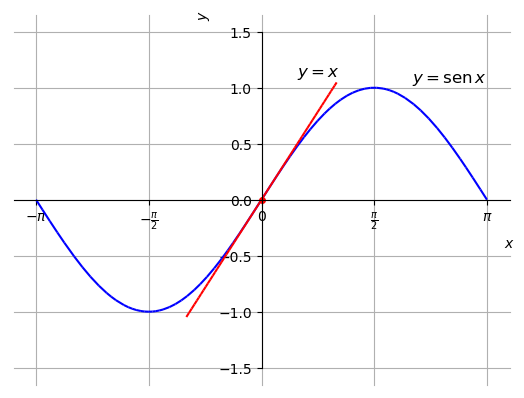
\includegraphics[width=0.7\textwidth]{./cap_deriv/dados/fig_deriv_exeresol_rt_sen0/fig_deriv_exeresol_rt_sen0}
    \caption{Esboços dos gráfico da função seno e de sua reta tangente no ponto $x=0$.}
    \label{fig:deriv_exeresol_rt_sen0}
  \end{figure}

  \ifispython
  Com o \sympy, podemos resolver este exercício com os seguintes comandos:
  \begin{lstlisting}
    from sympy import *
    x = Symbol('x')
    f = sin(x)
    x0 = 0

    # reta tangente
    rt = diff(f,x).subs(x,x0)*(x-x0)+f.subs(x,x0)
    print("Reta tangente: y = %s" % rt)

    # graficos
    plot(f,rt,(x,-pi,pi))
  \end{lstlisting}
  \fi  
\end{resol}

\begin{exeresol}
  Resolva a equação
  \begin{equation}
    \sec'(x) = 0,
  \end{equation}
  para $x\in \left(\frac{\pi}{2}, \frac{3\pi}{2}\right)$.
\end{exeresol}
\begin{resol}
  Temos
  \begin{align}
    0 &= \sec'(x) \\
      &= \sec(x)\tg(x) \\
      &= \frac{1}{\cos(x)}\frac{\sen(x)}{\cos(x)} \\
      &= \frac{\sen(x)}{\cos^2(x)}
  \end{align}
  donde segue que
  \begin{equation}
    \sen(x) = 0.
  \end{equation}
  Por fim, observamos que para $x\in \left(\frac{\pi}{2}, \frac{3\pi}{2}\right)$, a função seno se anula somente em $x=\pi$, a qual é a solução da equação.
\end{resol}


\subsection{Exercícios}

% \begin{flushright}
%   [Vídeo] | [Áudio] | \href{https://phkonzen.github.io/notas/contato.html}{[Contatar]}
% \end{flushright}

\begin{exer}
  Calcule a derivada em relação a $x$ de
  \begin{enumerate}[a)]
  \item $\displaystyle f(x)=\sen(x)-\cos^2(x)$
  \item $\displaystyle g(x)=\sen^2(x)\cos(x)$
  \item $\displaystyle h(x)=\frac{2\tg(x)}{\sec(x)}$
  \end{enumerate}
\end{exer}
\begin{resp}
  a)~$f'(x)=\sen(2x)+\cos(x)$; b)~$g'(x)=\sen(x)\cdot(2-3\sin^2(x)))$; c)~$h'(x)=2\cos(x)$
\end{resp}

\begin{exer}
  Encontre a equação da reta tangente ao gráfico da função $y = \cos x$ no ponto $x=0$. Então, faça os esboços desta função e da reta tangente, em uma mesma figura.  
\end{exer}
\begin{resp}
  $y = 1$. Dica: use um pacote de matemática simbólica para verificar os esboços dos gráficos.
\end{resp}

\begin{exer}
  Calcule a derivada em relação a $x$ de
  \begin{enumerate}[a)]
  \item $\displaystyle f(x)=\tg(x)-\cotg(x)$
  \item $\displaystyle g(x)=\sec(x)-\cossec(x)$
  \item $\displaystyle g(x)=\sec(x)-\cossec(x)$
  \end{enumerate}
\end{exer}
\begin{resp}
  a)~$f'(x)=\sec^2(x)+\cossec^2(x)$; b)~$g'(x)=\sec(x)\tg(x)+\cossec(x)\cotg(x)$; c)~$h'(x)=\frac{1}{2}\sec^2(x)$
\end{resp}


\section{Regra da cadeia}\label{cap_deriv_sec_cadeia}

\begin{flushright}
  [YouTube] | [Vídeo] | [Áudio] | \href{https://phkonzen.github.io/notas/contato.html}{[Contatar]}
\end{flushright}

Regra da cadeia é nome dado a técnica de derivação de uma função composta. Sejam $f$ e $g$, com $g$ derivável em $x$ e $f$ derivável em $g(x)$, então $(f\circ g)$ é derivável em $x$, sendo
\begin{equation}
  {\color{blue} (f\circ g)'(x) = [f(g(x))]' = f'(g(x))\cdot g'(x)},
\end{equation}
chamada de regra da cadeia.

\begin{ex}
  A derivada em relação a $x$ de $h(x) = (x+1)^2$ pode ser calculada das seguintes formas:
  \begin{enumerate}
  \item[a)] pela regra da cadeia.

    A função $h$ é a composição da função $f(x)=x^2$ com a função $g(x)=x+1$, i.e. $h(x) = f(g(x))$. Temos $f'(x)=2x$ e $g'(x)=1$. Então, segue pela regra da cadeia
    \begin{align}
      h'(x) &= [f(g(x))]' \\
            &= f'(g(x))\cdot g'(x) \\
            &= 2(x+1)\cdot 1 \\
            &= 2x+2.
    \end{align}

  \item[b)] por cálculo direto.

    Observando que $h(x)=(x+1)^2=x^2+2x+1$, temos
    \begin{align}
      h'(x) &= (x^2+2x+1)' \\
            &= (x^2)' + (2x)' + (1)' \\
            &= 2x + 2.
    \end{align}
  \end{enumerate}

  \ifispython
  Com o \sympy, temos:
  \begin{lstlisting}
    from sympy import *
    x = Symbol('x')
    diff((x+1)**2,x)
    2*x + 2
  \end{lstlisting}
  \fi  
\end{ex}

Usualmente, a regra da cadeia também é apresentada da seguinte forma
\begin{equation}\label{eq:deriv_regra_da_cadeia}
  {\color{blue}\frac{\dd}{\dd x}f(u) = f'(u)\frac{\dd u}{\dd x}},
\end{equation}
onde $u$ é uma função derivável em $x$ e $f$ é derivável em $u(x)$.

\begin{obs}\normalfont{(Derivada de função potência)}
  Em seções anteriores, já vimos que
  \begin{equation}
    \frac{\dd}{\dd x}x^n = nx^{n-1},
  \end{equation}
  para qualquer $n$ inteiro\footnote{Mais precisamente, para $n\neq 0$ e $n\neq 1$.}. Agora, se $r\neq 0$ e $r\neq 1$ é um número real, temos
  \begin{gather}
    y = x^r \\
    \ln y = \ln x^r = r\ln x.
  \end{gather}
  Daí, derivando ambos os lados desta última equação e observando que $y = y(x)$, obtemos
  \begin{gather}
    \frac{\dd}{\dd x} \ln y = \frac{\dd}{\dd x} r\ln x \\
    \frac{1}{y}\frac{\dd y}{\dd x} = \frac{r}{x} \\
    \frac{\dd y}{\dd x} = \frac{r}{x}y \\
    \frac{\dd y}{\dd x} = rx^{r-1}.
  \end{gather}
  Ou seja, a regra da potência
  \begin{equation}
    \frac{\dd}{\dd x}x^r = rx^{r-1},
  \end{equation}
  vale para todo $r$ real, com $r\neq 0$ e $r\neq 1$.
\end{obs}

\begin{ex}
  Vejamos os seguintes casos:
  \begin{enumerate}[a)]
  \item
    \begin{align}
      \frac{\dd}{\dd x}\sqrt{x} &= \left(x^{\frac{1}{2}}\right)' \\
                                &= \frac{1}{2}x^{\frac{1}{2}-1} \\
                                &= \frac{1}{2\sqrt{x}}.
    \end{align}
  \item
    \begin{align}
      \left(x^{\sqrt{2}}\right)' = \sqrt{2}x^{\sqrt{2}-1}.
    \end{align}
  \end{enumerate}
\end{ex}

\begin{obs}
  A regra da cadeia aplicada a derivada de função potência é
  \begin{equation}\label{eq:deriv_rcfp}
    \frac{\dd}{\dd x}u^r = ru^{r-1}\frac{\dd u}{\dd x}.
  \end{equation}
\end{obs}

\begin{ex}
  Vamos calcular a derivada em relação a $x$ de
  \begin{equation}
    f(x) = \sqrt{x^2+1}
  \end{equation}
  Vamos usar \eqref{eq:deriv_rcfp}, com
  \begin{equation}
    u = x^2 + 1
  \end{equation}
  e $r = 1/2$. Segue que
  \begin{align}
    f'(x) &= \frac{1}{2\sqrt{u}}\cdot \frac{d u}{d x} \\
          &= \frac{1}{2\sqrt{x^2+1}}\cdot 2x\\
          &= \frac{2x}{\sqrt{x^2+1}}
  \end{align}

  \ifispython
  No \sympy, temos:
\begin{lstlisting}
    from sympy import *
    x = Symbol('x')
    diff(sqrt(x**2+1),x)
    x/sqrt(x**2 + 1)
  \end{lstlisting}
  \fi  
\end{ex}

A regra da cadeia pode ser estendida para calcular a derivada de uma composição encadeada de três ou mais funções. Por exemplo,
\begin{align}
  [f(g(h(x)))]' &= f'(g(h(x)))\cdot[g(h(x))]' \\
                &= f'(g(h(x)))\cdot g'(h(x))\cdot h'(x).
\end{align}
Neste caso, a regra é válida para todo ponto tal que $h$ é derivável em $x$ com $g$ derivável em $h(x)$ e $f$ derivável em $f(g(h(x)))$.

\begin{ex}
  Vamos calcular a derivada em relação a $x$ de $f(x) = \sen(\cos(x^2))$. Pela regra da cadeia, temos
  \begin{align}
    [\sen(\cos(x^2))] &= \cos(\cos(x^2))\cdot[\cos(x^2)]' \\
                    &= \cos(\cos(x^2))\cdot [-\sen(x^2)\cdot (x^2)'] \\
                    &= -\cos(\cos(x^2))\cdot\sen(x^2)\cdot 2x.
  \end{align}

  \ifispython
  No \sympy, temos:
  \begin{lstlisting}
    from sympy import *
    x = Symbol('x')
    diff(sin(cos(x**2)))
    -2*x*sin(x**2)*cos(cos(x**2))
  \end{lstlisting}
  \fi  
\end{ex}

\subsection{Lista de derivadas}

\begin{align}
  & (ku)' = ku' \\
  & (u\pm v)' = u' \pm v'\\
  & (uv)' = u'v + uv' \\
  & \left(\frac{u}{v}\right)' = \frac{u'v - uv'}{v^2} \\
  & (k)' = 0 \\
  & (x)' = 1 \\
  & \frac{\dd u^n}{\dd x} = nu^{n-1}\frac{\dd u}{\dd x}\\
  & \frac{\dd a^u}{\dd x} = a^u\ln a\frac{\dd u}{\dd x} \\
  & \frac{\dd e^u}{\dd x} = e^u\frac{\dd u}{\dd x} \\
  & \frac{\dd}{\dd x}\log_a u = \frac{1}{u}\frac{\dd u}{\dd x}\\
  & \frac{\dd}{\dd x}\sen u = \cos(u)\frac{\dd u}{\dd x} \\
  & \frac{\dd}{\dd x}\cos u = - \sen(u)\frac{\dd u}{\dd x}\\
  & \frac{\dd}{\dd x}\tg u = \sec^2(u)\frac{\dd u}{\dd x} \\
  & \frac{\dd}{\dd x}\cotg u = -\cossec^2(u)\frac{\dd u}{\dd x} \\
  & \frac{\dd}{\dd x}\sec u = \sec(u)\tg(u)\frac{\dd u}{\dd x} \\
  & \frac{\dd}{\dd x}\cossec u = -\cossec(u)\cotg(u)\frac{\dd u}{\dd x}
\end{align}

\subsection{Exercícios resolvidos}

% \begin{flushright}
%   [Vídeo] | [Áudio] | \href{https://phkonzen.github.io/notas/contato.html}{[Contatar]}
% \end{flushright}

\begin{exeresol}
  Calcule a derivada em relação a $x$ de
  \begin{equation}
    f(x) = e^{\sqrt{x+1}}.
  \end{equation}
\end{exeresol}
\begin{resol}
  Da regra da cadeia aplicada à função exponencial, temos
  \begin{equation}
    \frac{\dd}{\dd x}e^u = e^u\frac{\dd u}{\dd x}.
  \end{equation}
  Então, com $u = \sqrt{x+1}$, segue
  \begin{align}
    f'(x) &= \frac{\dd}{\dd x}e^{\sqrt{x+1}} \\
          &= e^{\sqrt{x+1}}\frac{\dd}{\dd x}\left(\sqrt{x+1}\right).
  \end{align}
  Agora, aplicamos a regra da cadeia para a função raiz quadrada, i.e.
  \begin{equation}
    \frac{\dd}{\dd x}\sqrt{u} = \frac{1}{2\sqrt{u}}\frac{\dd u}{\dd x},
  \end{equation}
  com $u = x+1$. Segue, então
  \begin{align}
    \frac{\dd}{\dd x}\sqrt{x+1} &= \frac{1}{2}(x+1)^{\frac{1}{2}-1}\frac{\dd}{\dd x}(x+1) \\
                                &= \frac{1}{2\sqrt{x+1}}.
  \end{align}
  Portanto, concluímos que
  \begin{equation}
    f'(x) = \frac{1}{2\sqrt{x+1}}e^{\sqrt{x+1}}.
  \end{equation}

  \ifispython
  No \sympy, temos:
  \begin{lstlisting}
    from sympy import *
    x = Symbol('x')
    diff(exp(sqrt(x+1)),x)
    exp(sqrt(x + 1))/(2*sqrt(x + 1))
  \end{lstlisting}
  \fi  
\end{resol}

\begin{exeresol}
  Mostre que a \href{https://pt.wikipedia.org/wiki/Fun%C3%A7%C3%A3o_log%C3%ADstica}{função logística}
  \begin{equation}
    f(x) = \frac{1}{1+e^{-x}}
  \end{equation}
  satisfaz a equação diferencial
  \begin{equation}
    \frac{\dd}{\dd x}f(x) = f(x)(1-f(x)).
  \end{equation}
\end{exeresol}
\begin{resol}
  Vamos calcular a derivada em relação a $x$ da função logística, i.e.
  \begin{align}
    \frac{\dd}{\dd x}f(x) &= \frac{\dd}{\dd x}\left(\frac{1}{1+e^{-x}}\right) \\
          &= \frac{\dd}{\dd x}\left[\left(1+e^{-x}\right)^{-1}\right] \\
          &= -1\cdot\left(1+e^{-x}\right)^{-2}\cdot\underbrace{\left(1+e^{-x}\right)'}_{=-e^{-x}} \\
          &= \frac{e^{-x}}{\left(1+e^{-x}\right)^{2}}.
  \end{align}
  Por outro lado, temos
  \begin{align}
    f(x)(1-f(x)) &= \frac{1}{1+e^{-x}}\cdot\left(1 - \frac{1}{1+e^{-x}}\right) \\
                 &= \frac{1}{1+e^{-x}}\cdot\left(\frac{1+e^{-x}-1}{1+e^{-x}}\right) \\
                 &= \frac{e^{-x}}{\left(1+e^{-x}\right)^{2}}.
  \end{align}
  Ou seja, de fato temos
  \begin{equation}
    \frac{\dd}{\dd x}f(x) = f(x)(1-f(x)).
  \end{equation}  
\end{resol}

\begin{exeresol}
  Assuma que o custo de produção de uma unidade empresarial seja modelada pela função
  \begin{equation}
    c(x) = \sqrt{x-1} + e^{x-7},
  \end{equation}
  onde $c$ é o custo em função da produção $x$. Determine o custo marginal quando $x=3$.
\end{exeresol}
\begin{resol}
  O custo marginal é a função derivada do custo em relação à produção. Calculando, temos
  \begin{align}
    c'(x) &= \left(\sqrt{x-1} + e^{x-7}\right)\\
          &= \underbrace{\left(\sqrt{x-1}\right)'}_{(u^n)' = nu^{n-1}u'} + \underbrace{\left(e^{x-7}\right)'}_{(e^u)' = e^uu'}\\
          &= \frac{1}{2\sqrt{x-1}} + e^{x-7}.
  \end{align}
  Logo, o custo marginal quando $x=3$ é
  \begin{equation}
    c'(3) = \frac{1}{2\sqrt{3-1}} + e^{3-7} = \sqrt{2} + e^{-4}.
  \end{equation}
\end{resol}

\subsection{Exercícios}

% \begin{flushright}
%   [Vídeo] | [Áudio] | \href{https://phkonzen.github.io/notas/contato.html}{[Contatar]}
% \end{flushright}

\begin{exer}
  Calcule a derivada em relação a $x$ das seguintes funções
  \begin{enumerate}[a)]
  \item $\displaystyle f(x) = (2x-3)^{9}$
  \item $\displaystyle g(x) = \frac{1}{(2x-3)^{51}}$
  \item $\displaystyle h(x) = \sqrt{x^2+1}$
  \end{enumerate}
\end{exer}
\begin{resp}
  a)~$\displaystyle f'(x) = 18(2x-3)^8$; b)~$\displaystyle g'(x) = -\frac{102}{(2x-3)^{52}}$; c) $\displaystyle h'(x)=\frac{x}{\sqrt{x^2+1}}$
\end{resp}

\begin{exer}
  Calcule a derivada em relação a $x$ das seguintes funções
  \begin{enumerate}[a)]
  \item $\displaystyle f(x) = 2^{3x-1}$
  \item $\displaystyle g(x) = e^{-x^2}$
  \end{enumerate}
\end{exer}
\begin{resp}
  a)~$\displaystyle f'(x) = 3\cdot 2^{3x-1}\ln 2$; b)~$\displaystyle g'(x) = -2xe^{-x^2}$.
\end{resp}

\begin{exer}
  Calcule as seguintes derivadas
  \begin{enumerate}
  \item[a)] $\displaystyle\left[\ln\left(x^2-1\right)\right]'$ 
  \item[b)] $\displaystyle\frac{d}{dx}\left[\log_2(x-1) + \log_2(x+1)\right]$ 
  \end{enumerate}
\end{exer}
\begin{resp}
  a) $\displaystyle\frac{2x}{x^2-1}$; b) $\displaystyle\frac{2x}{(x^2-1)\ln 2}$
\end{resp}

\begin{exer}
  Calcule a derivada em relação a $x$ das seguintes funções
  \begin{enumerate}[a)]
  \item $\displaystyle f(x) = \sen(\pi x)$
  \item $\displaystyle g(x) = \cos(\sqrt{x})$
  \item $\displaystyle h(x) = \tg(2x)$
  \item $\displaystyle u(x) = \cotg(3 - x)$
  \item $\displaystyle v(x) = \sec\left(\frac{1}{x^2}\right)$
  \item $\displaystyle z(x) = \cossec\left(5x + x^2\right)$
  \end{enumerate}
\end{exer}
\begin{resp}
  a)~$\displaystyle f'(x) = \pi\cos(\pi x)$; b)~$\displaystyle g'(x) = -\frac{1}{2\sqrt{x}}\sen(\sqrt{x})$; c)~$\displaystyle h'(x) = 2\sec^2(2x)$; d)~$\displaystyle u'(x) = \cossec^2(3-x)$; e)~$\displaystyle v'(x) = -\frac{2}{x^2}\sec\left(\frac{1}{x^2}\right)\tg\left(\frac{1}{x^2}\right)$; f)~$\displaystyle z'(x) = -(5+2x)\cossec\left(5x + x^2\right)\cotg\left(5x + x^2\right)$
\end{resp}

\begin{exer}
  Encontre a equação da reta tangente ao gráfico da função
  \begin{equation}
    f(x) = e^{\sqrt{x+1}}
  \end{equation}
  no ponto $x=3$.
\end{exer}
\begin{resp}
  $y = \frac{e^2}{4}x + \frac{e^2}{4}$
\end{resp}

\section{Diferenciabilidade da função inversa}\label{cap_deriv_sec_funinv}

\begin{flushright}
  [YouTube] | [Vídeo] | [Áudio] | \href{https://phkonzen.github.io/notas/contato.html}{[Contatar]}
\end{flushright}

Seja $f$ uma função diferenciável e injetora em um intervalo aberto $I$. Então, pode-se mostrar que sua inversa $f^{-1}$ é diferenciável em qualquer ponto da imagem da $f$ no qual $f'(f^{-1}(x))\neq 0$ e sua derivada é
\begin{equation}\label{eq:diff_funinv}
  {\color{blue}\frac{d}{dx}[f^{-1}(x)] = \frac{1}{f'(f^{-1}(x))}}.
\end{equation}

\begin{ex}
  Seja $f(x) = (2x-1)^2$ para $x>1/2$. Para calcular sua inversa, fazemos
  \begin{gather}
    y = (2x-1)^2 \\
    \sqrt{y} = 2x-1 \\
    x = \frac{\sqrt{y}+1}{2}
  \end{gather}
  Ou seja,
  \begin{equation}
    f^{-1}(x) = \frac{1}{2}(\sqrt{x}+1).
  \end{equation}
  Calculando a derivada de $f^{-1}$ diretamente, temos
  \begin{align}
    \frac{\dd}{\dd x}f^{-1}(x) &= \frac{1}{2}\left(\sqrt{x}+1\right)' \\
                               &= \frac{1}{2}\cdot\frac{1}{2\sqrt{x}} \\
                               &= \frac{1}{4\sqrt{x}}
  \end{align}
  Agora, usando \eqref{eq:diff_funinv} e observando que $f'(x) = 8x-4$, obtemos
  \begin{align}
    \frac{\dd}{\dd x}f^{-1}(x) &= \frac{1}{f'(f^{-1}(x))},\\
                               &= \frac{1}{8\cdot \frac{1}{2}\left(\sqrt{x}+1\right)-4}, \\
                               &= \frac{1}{4\sqrt{x}},
  \end{align}
  como esperado.
\end{ex}

\begin{obs}\normalfont{(Derivada da função logarítmica)}
  \begin{itemize}
  \item Tomando $f(x) = e^x$ temos $f^{-1}(x) = \ln x$ e, daí por \eqref{eq:diff_funinv}
    \begin{equation}
      \frac{\dd }{\dd x}\ln x = \frac{1}{e^{\ln x}} = \frac{1}{x}.
    \end{equation}
  \item Tomando $f(x) = a^x$, $a> 0$ e $a\neq 1$, temos $f^{-1}(x) = \log_a x$ e, por \eqref{eq:diff_funinv},
    \begin{equation}
      \frac{\dd}{\dd x}\log_a x = \frac{1}{a^{\log_a x}\ln a} = \frac{1}{x\ln a}.
    \end{equation}
  \end{itemize}
\end{obs}

\begin{ex}
  Vamos calcular a derivada em relação a $x$ da função
  \begin{equation}
    f(x) = \ln \frac{1}{x}.
  \end{equation}
  Aplicando a regra da cadeia na derivada da função logarítmica, temos
  \begin{equation}
    \frac{\dd}{\dd x}\ln u = \frac{1}{u}\frac{\dd u}{\dd x}.
  \end{equation}
  Portanto, temos
  \begin{align}
    f'(x) &= \left(\ln\frac{1}{x}\right)'\\
          &= \frac{1}{x^{-1}}\cdot (-x^{-2}) \\
          &= -\frac{1}{x}.
  \end{align}

  \ifispython
  No \sympy, temos:
  \begin{lstlisting}
    from sympy import *
    x = Symbol('x')
    diff(log(1/x),x)
    -1/x
  \end{lstlisting}
  \fi  
\end{ex}

\subsection{Derivadas de funções trigonométricas inversas}

\begin{flushright}
  [Vídeo] | [Áudio] | \href{https://phkonzen.github.io/notas/contato.html}{[Contatar]}
\end{flushright}

Seja $f(x) = \sen x$ restrita a $-\pi/2 \leq x \leq \pi/2$. Sua inversa é a função arco seno, denotada por
\begin{equation}
  y = \arc\sen x.
\end{equation}

\begin{figure}[H]
  \centering
  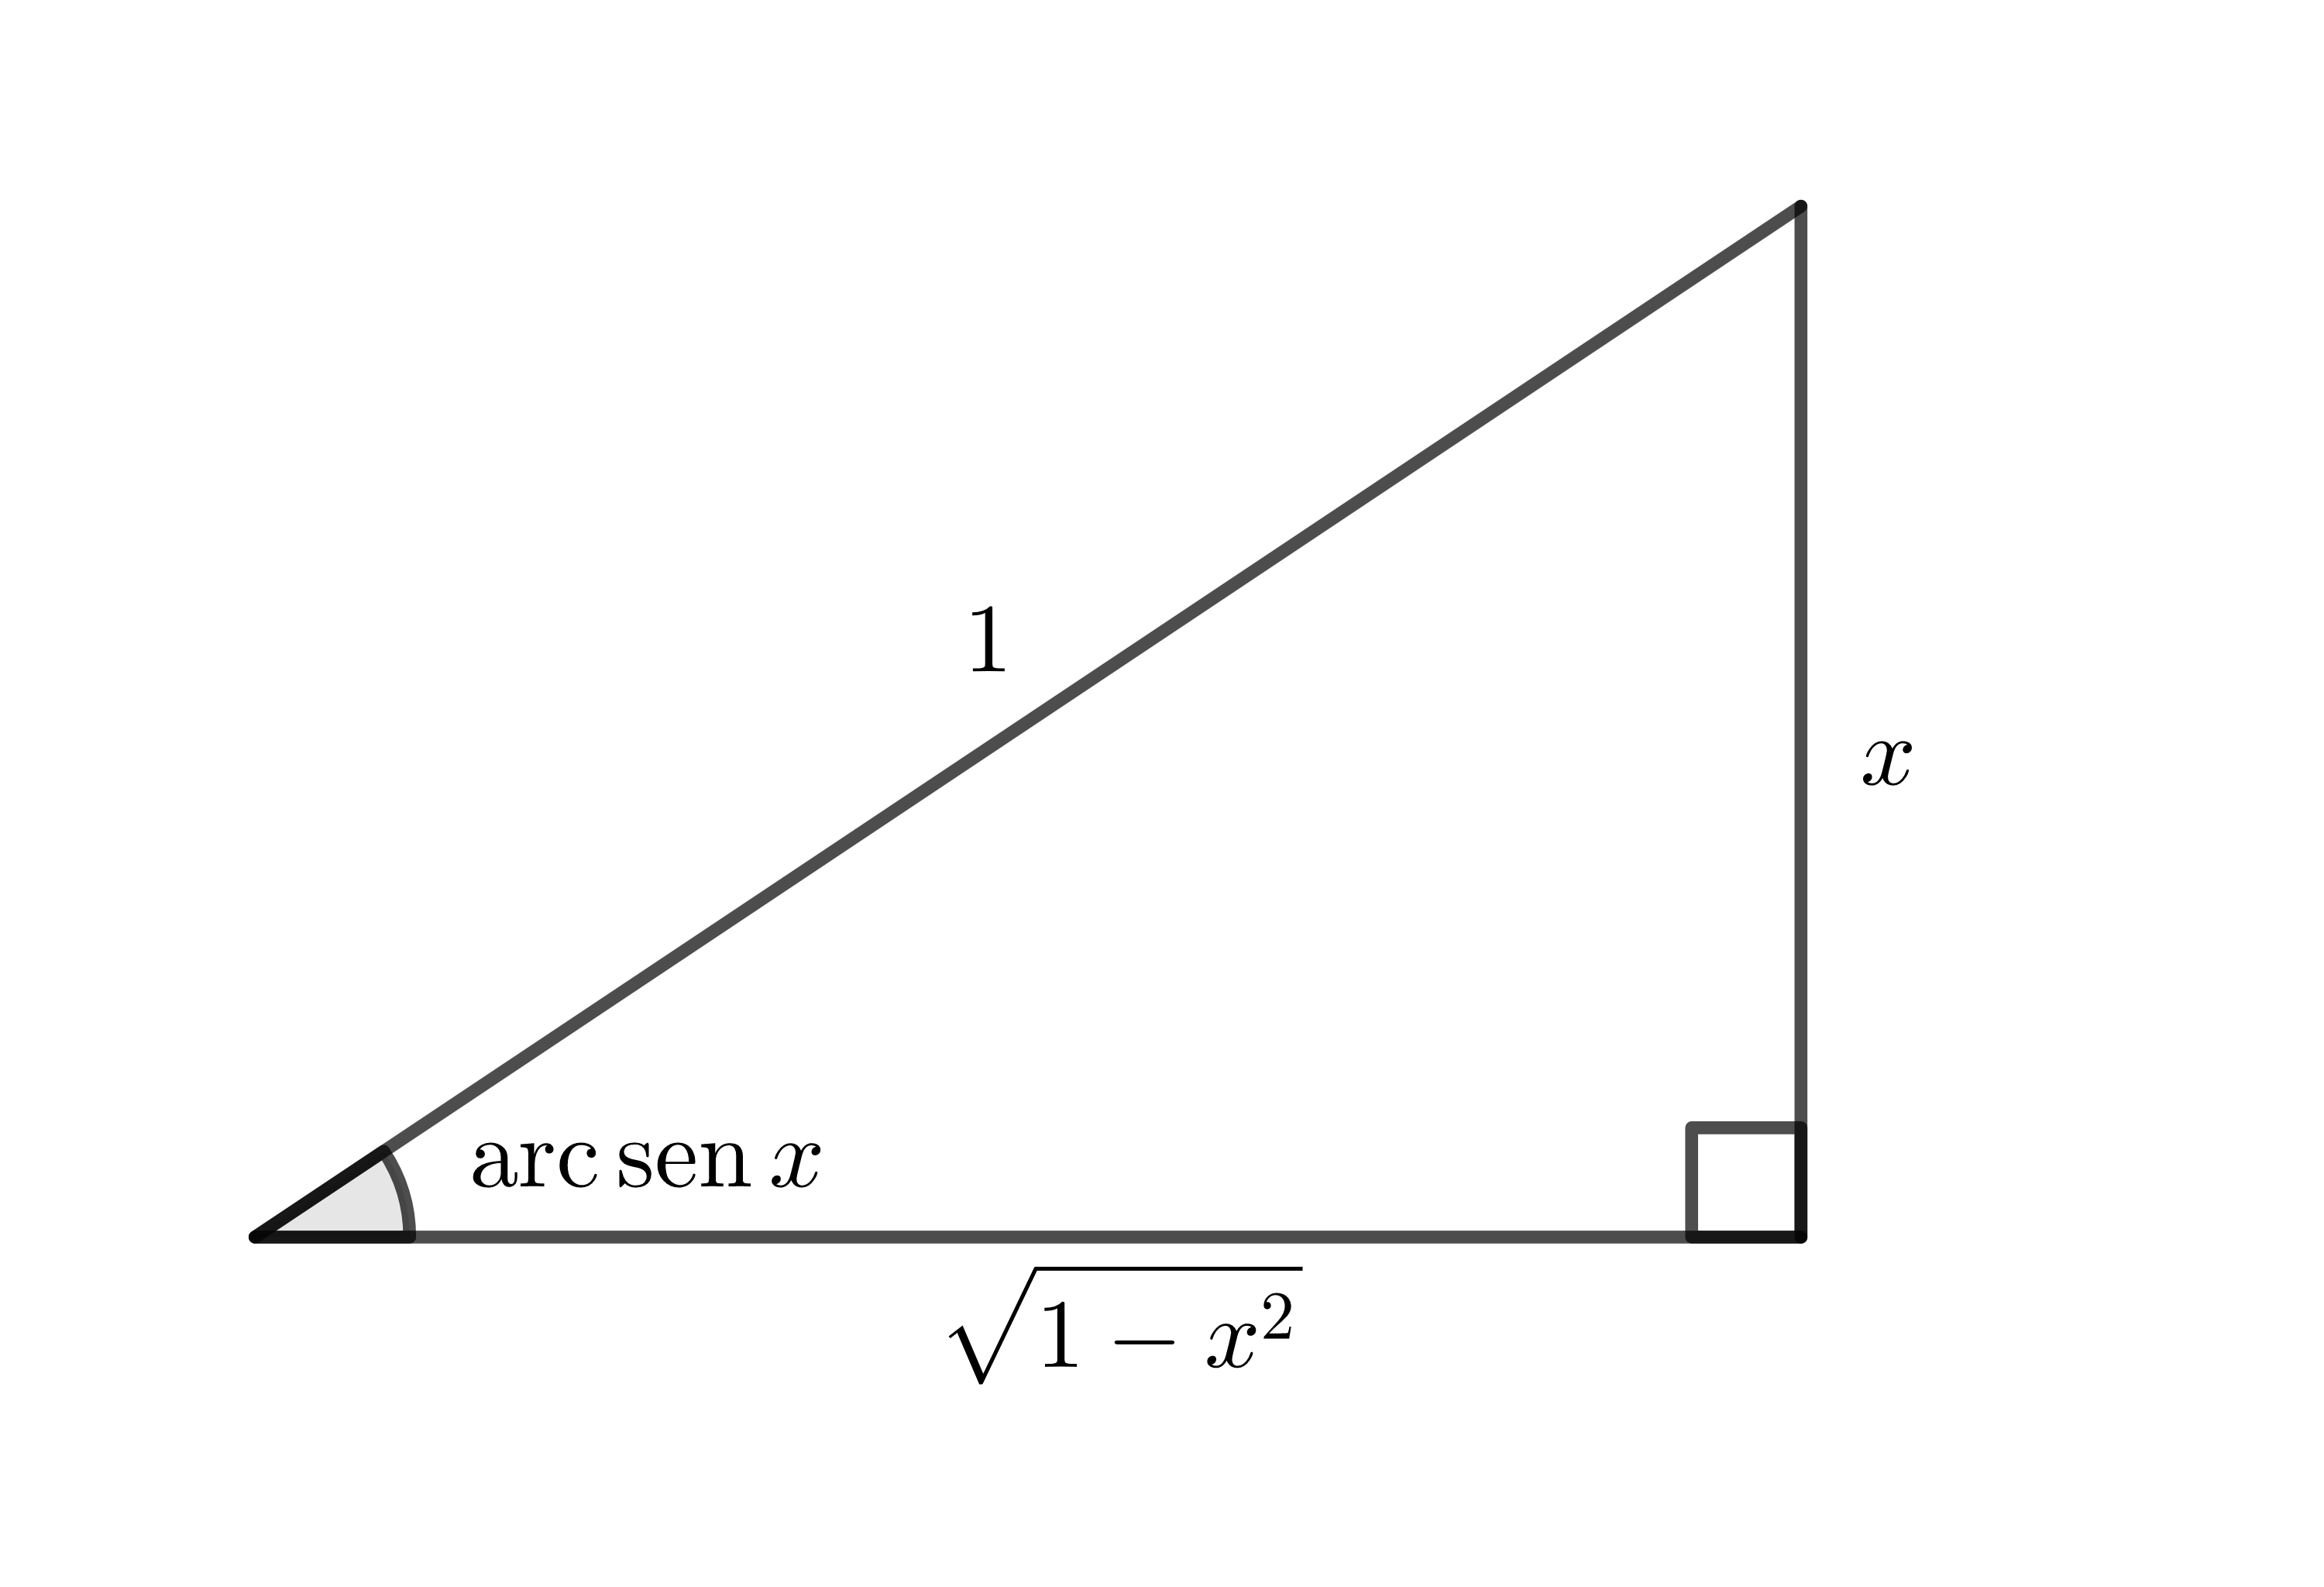
\includegraphics[width=0.5\textwidth]{./cap_deriv/dados/fig_diff_arc_sen/fig_diff_arc_sen}
  \caption{Arco seno de um ângulo no triângulo retângulo.}
  \label{fig:diff_arc_sen}
\end{figure}

Para calcular a derivada da função arco seno, vamos usar \eqref{eq:diff_funinv} com $f(x)=\sen x$ e $f'(x) = \arc\sen x$, donde
\begin{equation}
  (\arc\sen x)' = \frac{1}{\cos(\arc\sen x)}.
\end{equation}
Como $\cos(\arc\sen x) = \sqrt{1-x^2}$ (veja Figura \ref{fig:diff_arc_sen}), concluímos
\begin{equation}
  (\arc\sen x)' = \frac{1}{\sqrt{1-x^2}}.
\end{equation}


\begin{ex}
  A regra da cadeia aplicada à derivada da função arco seno é
  \begin{equation}
    \frac{\dd}{\dd x}\arc\sen u = \frac{1}{\sqrt{1-u^2}}\frac{\dd u}{\dd x}.
  \end{equation}

  Por exemplo, temos
  \begin{equation}
    \frac{\dd}{\dd x}\arc\sen x^2 = \frac{2x}{\sqrt{1-x^4}}.
  \end{equation}

  \ifispython
  No \sympy, temos:
  \begin{lstlisting}
    from sympy import *
    x = Symbol('x')
    diff(asin(x**2),x)
    2*x/sqrt(-x**4 + 1)
  \end{lstlisting}
  \fi    
\end{ex}

Com argumentos análogos aos usados no cálculo da derivada da função arco seno, podemos obter as seguintes derivadas:
\begin{align}
  & (\arc\cos x)' = -\frac{1}{\sqrt{1-x^2}} & \\
  &(\arc\tg x)' = \frac{1}{1+x^2} \\
  & (\arc\cotg x)' = -\frac{1}{1+x^2} \\
  & (\arc\sec x)' = \frac{1}{|x|\sqrt{x^2-1}} \\
  & (\arc\cosec x)' = -\frac{1}{|x|\sqrt{x^2-1}}
\end{align}

\begin{ex}
  A regra da cadeia aplicada a função arco tangente é
  \begin{equation}
    \frac{\dd}{\dd x}\arc\tg u = \frac{1}{1+u^2}\frac{\dd u}{\dd x}.
  \end{equation}

  Por exemplo, temos
  \begin{align}
    \frac{\dd}{\dd x}\arc\tg\sqrt{x} &= \frac{1}{1+(\sqrt{x})^2}\frac{\dd}{\dd x}\sqrt{x} \\
                                     &=  \frac{1}{2(1+x)\sqrt{x}}.
  \end{align}

  \ifispython
  No \sympy, temos:
  \begin{lstlisting}
    from sympy import *
    x = Symbol('x')
    diff(atan(sqrt(x)))
    1/(2*sqrt(x)*(x + 1))
  \end{lstlisting}
  \fi    
\end{ex}

\subsection{Lista de derivadas}\label{deriv_tabela_de_derivadas}

\begin{flushright}
  [Vídeo] | [Áudio] | \href{https://phkonzen.github.io/notas/contato.html}{[Contatar]}
\end{flushright}

\begin{align}
  & (ku)' = ku' \\
  & (u\pm v)' = u' \pm v'\\
  & (uv)' = u'v + uv' \\
  & \left(\frac{u}{v}\right)' = \frac{u'v - uv'}{v^2} \\
  & (k)' = 0 \\
  & (x)' = 1 \\
  & \frac{\dd}{\dd x}u^r = ru^{r-1}\frac{\dd u}{\dd x}\\
  & \frac{\dd}{\dd x}a^u = a^u\ln a\frac{\dd u}{\dd x} \\
  & \frac{\dd}{\dd x}e^u = e^u\frac{\dd u}{\dd x} \\
  & \frac{\dd}{\dd x}\log_a u = \frac{1}{u\ln a}\frac{\dd u}{\dd x} \\
  & \frac{\dd}{\dd x}\ln u = \frac{1}{u}\frac{\dd u}{\dd x} \\
  & \frac{\dd}{\dd x}\sen u = \cos(u)\frac{\dd u}{\dd x} \\
  & \frac{\dd}{\dd x}\cos u = - \sen(u)\frac{\dd u}{\dd x}\\
  & \frac{\dd}{\dd x}\tg u = \sec^2(u)\frac{\dd u}{\dd x} \\
  & \frac{\dd}{\dd x}\cotg u = -\cossec^2(u)\frac{\dd u}{\dd x} \\
  & \frac{\dd}{\dd x}\sec u = \sec(u)\tg(u)\frac{\dd u}{\dd x} \\
  & \frac{\dd}{\dd x}\cossec u = -\cossec(u)\cotg(u)\frac{\dd u}{\dd x} \\
  &\frac{\dd}{\dd x}\arc\sen u = \frac{1}{\sqrt{1-u^2}}\frac{\dd u}{\dd x} \\
  & \frac{\dd}{\dd x}\arc\cos u = -\frac{1}{\sqrt{1-u^2}}\frac{\dd u}{\dd x} \\
  &\frac{\dd}{\dd x}\arc\tg u = \frac{1}{1+u^2}\frac{\dd u}{\dd x} \\
  & \frac{\dd}{\dd x}\arc\cotg u = -\frac{1}{1+u^2}\frac{\dd u}{\dd x} \\
  &\frac{\dd}{\dd x}\arc\sec u = \frac{1}{|u|\sqrt{u^2-1}}\frac{\dd u}{\dd x} \\
  & \frac{\dd}{\dd x}\arc\cossec u = -\frac{1}{|u|\sqrt{u^2-1}}\frac{\dd u}{\dd x}
\end{align}

\subsection{Exercícios resolvidos}

% \begin{flushright}
%   [Vídeo] | [Áudio] | \href{https://phkonzen.github.io/notas/contato.html}{[Contatar]}
% \end{flushright}

\begin{exeresol}
  Calcule a equação da reta tangente ao gráfico da função $f(x) = \ln x$ no ponto $x=1$. Faça, então, um esboço dos gráficos da função e da reta tangente.
\end{exeresol}
\begin{resol}
  A equação da reta tangente ao gráfico da função $f(x) = \ln x$ no ponto $x_0=1$ é
  \begin{gather}
    y = f'(x_0)(x-x_0)+f(x_0) \\
    y = f'(1)(x-1)+f(1).
  \end{gather}
  Observando que
  \begin{equation}
    f'(x) = (\ln x)' = \frac{1}{x},
  \end{equation}
  temos que a equação da reta tangente é
  \begin{gather}
    y = \frac{1}{1}(x-1)+\ln 1 \\
    y = x-1.
  \end{gather}
  Na Figura \ref{fig:deriv_exeresol_rt_ln}, temos um esboço dos gráficos da função e da reta tangente.

  \begin{figure}[H]
    \centering
    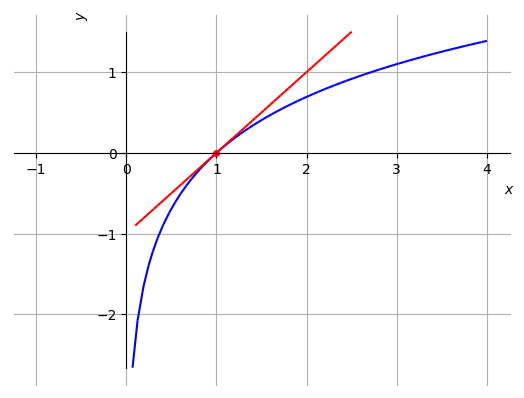
\includegraphics[width=0.7\textwidth]{./cap_deriv/dados/fig_deriv_exeresol_rt_ln/fig_deriv_exeresol_rt_ln}
    \caption{Esboço dos gráficos da função logarítmica natural e da reta tangente no ponto $x=1$.}
    \label{fig:deriv_exeresol_rt_ln}
  \end{figure}

  \ifispython
  No \sympy, temos:
  \begin{lstlisting}
    from sympy import *
    x = Symbol('x')
    rt = diff(log(x)).subs(x,1)*(x-1)+log(1)
    print("y = %s" % rt)
    y = x - 1
  \end{lstlisting}
  \fi    
\end{resol}

\begin{exeresol}
  Resolva a equação
  \begin{equation}
    \frac{\dd}{\dd x}\arc\tg x = 1.
  \end{equation}
\end{exeresol}
\begin{resol}
  Lembrando que
  \begin{equation}
    \frac{\dd}{\dd x}\arc\tg x = \frac{1}{1+x^2},
  \end{equation}
  temos
  \begin{gather}
    \frac{\dd}{\dd x}\arc\tg x = 1 \\
    \frac{1}{1+x^2}=1 \\
    1+x^2 = 1 \\
    x^2 = 0 \\
    x = 0.
  \end{gather}
\end{resol}

\begin{exeresol}
  Calcule
  \begin{equation}
    \frac{\dd}{\dd x}x^x.
  \end{equation}
\end{exeresol}
\begin{resol}
  Observamos que
  \begin{gather}
    y = x^x \\
    \ln y = \ln x^x \\
    \ln y = x\ln x.
  \end{gather}
  Agora, derivando em relação a $x$ ambos os lados desta equação, obtemos
  \begin{gather}
    \frac{\dd}{\dd x}\ln y = \frac{\dd}{\dd x}\left(x\ln x\right) \\
    \frac{1}{y}\frac{\dd y}{\dd x} = 1 + \ln x \\
    \frac{\dd y}{\dd x} = y(1 + \ln x) \\
    \frac{\dd x^x}{\dd x} = x^x(1 + \ln x).
  \end{gather}
\end{resol}

\subsection{Exercícios}

% \begin{flushright}
%   [Vídeo] | [Áudio] | \href{https://phkonzen.github.io/notas/contato.html}{[Contatar]}
% \end{flushright}

\begin{exer}
  Calcule a derivada em relação a $x$ das seguintes funções:
  \begin{enumerate}[a)]
  \item $f(x) = \log_2 x^2$
  \item $g(x) = \ln (xe^x)$
  \end{enumerate}
\end{exer}
\begin{resp}
  a)~$\displaystyle f'(x) = \frac{2}{x\ln 2}$; b)~$g'(x) = \frac{1+x}{x}$
\end{resp}

\begin{exer}
  Calcule a derivada em relação a $x$ das seguintes funções:
  \begin{enumerate}[a)]
  \item $f(x) = \sqrt[3]{x^2}$
  \item $g(x) = (1+2x)^e$
  \end{enumerate}
\end{exer}
\begin{resp}
  a)~$\displaystyle f'(x) = \frac{2}{3\sqrt[3]{x}}$; b)~$g'(x) = 2e(1+2x)^{e-1}$
\end{resp}

\begin{exer}
  Calcule
  \begin{equation}
    \frac{\dd}{\dd x} (1+x)^x.
  \end{equation}
\end{exer}
\begin{resp}
  $x(1+x)^{x-1} + (1+x)^x\ln(1+x)$
\end{resp}

\begin{exer}
  Encontre a equação da reta tangente ao gráfico de $f(x) = \arc\tg x$ no ponto $x=0$.
\end{exer}
\begin{resp}
  $y=x$
\end{resp}

\section{Derivação implícita}\label{cap_deriv_sec_derimp}

\begin{flushright}
  [Vídeo] | [Áudio] | \href{https://phkonzen.github.io/notas/contato.html}{[Contatar]}
\end{flushright}

Seja $y = y(x)$ definida implicitamente por
\begin{equation}
  g(y(x)) = 0.
\end{equation}
A derivada $\dd y/\dd x$ pode ser calculada via regra da cadeia
\begin{gather}
  \frac{\dd}{\dd x}g(y(x)) = \frac{\dd 0}{\dd x} \\
  g'(y(x))\frac{\dd y}{\dd x} = 0.
\end{gather}

\begin{ex}\label{ex:derivimp_cric}
  Considere a equação da circunferência unitária
  \begin{equation}\label{eq:deriv_circ}
    x^2 + y^2 = 1.
  \end{equation}
  Aqui, vamos calcular $\dd y/\dd x$ de duas maneiras diferentes.

  \begin{figure}[H]
    \centering
    \includegraphics[width=0.7\textwidth]{./cap_deriv/dados/fig_circ/fig}
    \caption{Esboço do gráfico da circunferência unitária $x^2 + y^2 = 1$.}
    \label{fig:circ}
  \end{figure}

  \begin{enumerate}[a)]
  \item Por derivação direta. Isolando $y$ em \eqref{eq:deriv_circ}, temos
    \begin{equation}
      y = \pm \sqrt{1 - x^2}
    \end{equation}
    o que está bem definido para $-1\leq x \leq 1$. Calculando a derivada, obtemos
    \begin{align}
      \frac{\dd y}{\dd x} &= \frac{\dd}{\dd x}\left(\pm\sqrt{1 - x^2}\right)\\
                          &= \pm\frac{-2x}{2\sqrt{1-x^2}}\\
                          &= \mp \frac{x}{y}
    \end{align}
    Ou seja, para $y < 0$, temos $y' = x/y$ e, para $y>0$, temos $y' = -x/y$. Logo, concluímos que
    \begin{equation}
      \frac{\dd y}{\dd x} = -\frac{x}{y}.
    \end{equation}
  \item Por derivação implícita. Derivamos ambos os lados da \eqref{eq:deriv_circ} em relação a $x$
    \begin{gather}
      \frac{\dd}{\dd x}\left(x^2+y^2\right) = \frac{\dd 1}{\dd x} \\
      \frac{\dd}{\dd x}\left(x^2\right) + \frac{\dd}{\dd x}\left(y^2(x)\right) = 0\\
      2x + \frac{\dd y^2}{\dd y}\frac{\dd y}{\dd x} = 0\\
      2x + 2y\frac{\dd y}{\dd x} = 0\\
      \frac{\dd y}{\dd x} = -\frac{x}{y}.
    \end{gather}
  \end{enumerate}
\end{ex}

\begin{obs}[Derivadas de potências racionais de $x$]
  Vamos mostrar que
  \begin{equation}
    {\color{blue}\frac{\dd}{\dd x}x^r = rx^{r-1}},
  \end{equation}
  para qualquer \emph{número racional} $r\neq 0$. Denotando $r = m/n$, $m,n\in\mathbb{N}$, temos
  \begin{gather}
    y = x^{m/n}\\
    \Leftrightarrow\\
    y^n = x^m
  \end{gather}
  Da derivação de função potência com exponente inteiro, temos
  \begin{gather}
    \frac{\dd}{\dd x}y^n = \frac{\dd}{\dd x}x^m\\
    ny^{n-1}\frac{\dd y}{\dd x} = mx^{m-1}\\
    \frac{\dd y}{\dd x} = \frac{m}{n}x^{m-1}y^{1-n}\\
    \frac{\dd y}{\dd x} = \frac{m}{n}x^{m-1}\left(x^{\frac{m}{n}}\right)^{1-n}\\
    \frac{\dd y}{\dd x} = \frac{m}{n}x^{m-1}x^{\frac{m}{n}(1-n)}\\
    \frac{\dd y}{\dd x} = \frac{m}{n}x^{m-1 + \frac{m}{n}(1-n)}\\
    \frac{\dd y}{\dd x} = \frac{m}{n}x^{\frac{m}{n}-1}.
  \end{gather}
  Logo, segue o resultados que queríamos demonstrar.
\end{obs}

\begin{ex}
  Vamos calcular $\displaystyle \frac{\dd^2 y}{\dd x^2}$ para
  \begin{equation}
    x^2 + y^2 = 1.
  \end{equation}
  Primeiramente, precisamos calcular $\dd y/\dd x$. Isso foi feito no Exemplo \ref{ex:derivimp_cric}, onde obtivemos
  \begin{equation}
    \frac{\dd y}{\dd x} = -\frac{x}{y}.
  \end{equation}
  Antes de derivarmos novamente, vamos reescrever essa última expressão da seguinte forma
  \begin{equation}
    y\frac{\dd y}{\dd x} = -x
  \end{equation}
  Derivando
  \begin{gather}
    \frac{\dd}{\dd x}\left[y\frac{\dd y}{\dd x}\right] = \frac{\dd}{\dd x}\left[-x\right]\\
    1\frac{\dd y}{\dd x}\frac{\dd y}{\dd x} + \frac{\dd}{\dd x}\frac{\dd y}{\dd x} = -1\\
    \left(\frac{\dd y}{\dd x}\right)^2 + \frac{\dd^2 y}{\dd x^2} = -1\\
    \frac{\dd^2 y}{\dd x^2} = -\frac{x^2}{y^2} - 1.
  \end{gather}
\end{ex}

\subsection{Exercícios resolvidos}

\begin{exeresol}
  Calcule $\dd y/\dd x$ para a lemniscata de Bernoulli\footnote{Jacob Bernoulli, 1655 - 1705, matemático suíço. Fonte: \href{https://pt.wikipedia.org/wiki/Jakob_Bernoulli}{Wikipédia}.}
  \begin{equation}
    (x^2 + y^2)^2 = x^2 - y^2.
  \end{equation}
  \begin{figure}[H]
    \centering
    \includegraphics[width=0.7\textwidth]{./cap_deriv/dados/fig_lemniscata/fig}
    \caption{Esboço da lemniscata de Bernoulli $(x^2+y^2)^2 = x^2 - y^2$.}
    \label{fig:lemniscata}
  \end{figure}
\end{exeresol}
\begin{resol}
  \begin{gather}
    \frac{\dd}{\dd x}\left[(x^2 + y^2)^2\right] = \frac{\dd}{\dd x}\left[x^2 - y^2\right]\\
    2(x^2 + y^2)\left(2x + 2y\frac{\dd y}{\dd x}\right) = 2x - 2y\frac{\dd y}{\dd x}
  \end{gather}
  Rearranjando os termos, obtemos
  \begin{equation}
    2(y + 2x^2y + 2y^2)\frac{\dd y}{\dd x} = 2x - 4xy^2 - 4x^3
  \end{equation}
  ou ainda
  \begin{equation}
    \frac{\dd y}{\dd x} = \frac{x - 2x^3 - 2xy^2}{y + 2x^2y + 2y^3}
  \end{equation}
\end{resol}

\begin{exeresol}
  Calcule a equação da reta tangente ao gráfico da circunferência unitária
  \begin{equation}
    x^2 + y^2 = 1
  \end{equation}
  no ponto $\displaystyle\left(\frac{\sqrt{2}}{2}, \frac{\sqrt{2}}{2}\right)$.
\end{exeresol}
\begin{resol}
  A equação da reta tangente ao gráfico de uma função $y = y(x)$ no ponto $(x_0, y(x_0))$ é dada por
  \begin{equation}
    y = y'(x_0)(x - x_0) + y(x_0)
  \end{equation}
  onde, nesse caso, $\displaystyle x_0 = \frac{\sqrt{2}}{2}$, $\displaystyle y(x_0) = \frac{\sqrt{2}}{2}$
  \begin{equation}
    y'(x_0) = \left.\frac{\dd y}{\dd x}\right|_{x=x_0}.
  \end{equation}
  Calculamos $\dd y/\dd x$ como segue
  \begin{gather}
    \frac{\dd}{\dd x}\left(x^2+y^2\right) = \frac{\dd 1}{\dd x} \\
    \frac{\dd}{\dd x}\left(x^2\right) + \frac{\dd}{\dd x}\left(y^2(x)\right) = 0\\
    2x + \frac{\dd y^2}{\dd y}\frac{\dd y}{\dd x} = 0\\
    2x + 2y\frac{\dd y}{\dd x} = 0\\
    \frac{\dd y}{\dd x} = -\frac{x}{y}.
  \end{gather}
  Com isso, temos
  \begin{align}
    y'(x_0) &= -\frac{x_0}{y(x_0)}\\
            &= -\frac{\frac{\sqrt{2}}{2}}{\frac{\sqrt{2}}{2}}\\
            &= -1.
  \end{align}
  Concluímos que a equação da reta tangente é
  \begin{gather}
    y = -1\cdot \left(x - \frac{\sqrt{2}}{2}\right) + \frac{\sqrt{2}}{2}\\
    y = -x + \sqrt{2}.
  \end{gather}
\end{resol}

\subsection{Exercícios}

\begin{exer}
  Calcule $\dd y/\\d x$ para:
  \begin{enumerate}[a)]
  \item $x + 2xy - x^3 = 3$
  \item $x^2 + y^2 = xy$
  \end{enumerate}
\end{exer}
\begin{resp}
  a) $\displaystyle \frac{\dd y}{\dd x} = \frac{3x^2 - 2y - 1}{2x}$ b) $\displaystyle \frac{\dd y}{\dd x} = \frac{y - 2x}{2y - x}$
\end{resp}

\begin{exer}
  Calcule $\dd^2 y/\dd x^2$ para
  \begin{equation}
    x^2 + y^2 = xy
  \end{equation}
\end{exer}
\begin{resp}
  $\displaystyle \frac{\dd^2 y}{\dd x^2} = \frac{x + y - 2}{x^2}$
\end{resp}  

\begin{exer}
  Encontre o ponto de interseção das retas tangentes ao gráfico de
  \begin{equation}
    y^2  = x - 1
  \end{equation}
  nos pontos $(2, -1)$ e $(2, 1)$.
\end{exer}
\begin{resp}
  (0, 0)
\end{resp}

\begin{exer}
  Encontre a equação da reta tangente ao gráfico da circunferência de centro $C = (1,1)$ e raio $r=\sqrt{2}$ que passa pela origem $O = (0,0)$.  
\end{exer}
\begin{resp}
  $y = -x$
\end{resp}

\begin{exer}
  Seja $c$ a circunferência de raio $r> 0$
  \begin{equation}
    x^2 + y^2 = r^2.
  \end{equation}
  Mostra que a reta tangente ao gráfico de $c$ em qualquer ponto arbitrário $P = (x_0, y_0)\in c$ é perpendicular a reta $\overline{OP}$, i.e. a reta que passa pela origem $O = (0, 0)$ e pelo ponto $P.$
\end{exer}



\chapter{Aplicações da derivada}\label{cap_apderiv}

\ifispython
\begin{obs}\label{obs:cap_apderiv_python}
  Nos códigos \sympy~ apresentados neste capítulo, assumimos o seguinte preâmbulo:
\begin{verbatim}
from sympy import *
var('x',real=True)
\end{verbatim}
\end{obs}
\fi

\section{Regra de L'Hôpital}\label{cap_apderiv_sec_lhospital}

\begin{flushright}
  [Vídeo] | [Áudio] | \href{https://phkonzen.github.io/notas/contato.html}{[Contatar]}
\end{flushright}

A regra de L'Hôpital é uma técnica para o cálculo de limites de indeterminações. Sejam $f$ e $g$ funções deriváveis em um intervalo aberto contendo $x=a$, exceto possivelmente em $x=a$, e
\begin{equation}
  \lim_{x\to a} f(x) = 0\quad\text{e}\quad\lim_{x\to a} g(x) = 0.
\end{equation}
Se, ainda, $\lim_{x\to a} f(x)/g(x)$ existe ou for $\pm\infty$, então
\begin{equation}
  \lim_{x\to a} \frac{f(x)}{g(x)} = \lim_{x\to a} \frac{f'(x)}{g'(x)}.
\end{equation}
Esta é a versão da regra de L'Hôpital para indeterminações do tipo $0/0$. Sem grandes modificações, é diretamente estendida para os casos $x\to a^-$, $x\to a^+$, $x\to \infty$ e $x\to -\infty$.

\begin{ex}
  Vamos calcular o limite
  \begin{equation}
    \lim_{x\to 1} \frac{x-1}{x^2-1}.
  \end{equation}
  \begin{enumerate}[a)]
  \item Pela regra de L'Hôpital.
    \begin{align}
      \lim_{x\to 1} \frac{x-1}{x^2-1} &= \lim_{x\to 1} \frac{(x+1)'}{(x^2-1)'} \\
                                      &= \lim_{x\to 1} \frac{1}{2x} \\
                                      &= \frac{1}{2}.
    \end{align}
  \item Por eliminação do fator comum.
    \begin{align}
      \lim_{x\to 1} \frac{x-1}{x^2-1} &= \lim_{x\to 1} \frac{x-1}{(x-1)(x+1)} \\
                                      &= \lim_{x\to 1} \frac{1}{x+1} \\
                                      &= \frac{1}{2}.
    \end{align}
  \end{enumerate}

  \ifispython
  No \sympy\footnote{Veja a Observação \ref{obs:cap_apderiv_python}.}, temos
\begin{verbatim}
>>> limit((x-1)/(x**2-1),x,1)
1/2
\end{verbatim}
  \fi
\end{ex}

\begin{ex}
  O limite
  \begin{equation}
    \lim_{x\to 2} \frac{x^2-4x+4}{x^3-3x^2+4}
  \end{equation}
  é uma indeterminação $0/0$. Aplicando a regra de L'Hôpital, obtemos
  \begin{equation}
    \lim_{x\to 2} \frac{x^2-4x+4}{x^3-3x^2+4} = \lim_{x\to 2} \frac{\cancelto{0}{2x-4}}{\cancelto{0}{3x^2-6x}},
  \end{equation}
  que também é uma indeterminação do tipo $0/0$. Agora, aplicando a regra de L'Hôpital novamente, obtemos
  \begin{equation}
    \lim_{x\to 2} \frac{2x-4}{3x^2-6x} = \lim_{x\to 2} \frac{2}{6x-6} = \frac{1}{3}.
  \end{equation}
  Portanto, concluímos que
  \begin{equation}
    \lim_{x\to 2} \frac{x^2-4x+4}{x^3-3x^2+4} = \frac{1}{3}.
  \end{equation}  

  \ifispython
  No \sympy\footnote{Veja a Observação \ref{obs:cap_apderiv_python}.}, temos
\begin{verbatim}
>>> limit((x**2-4*x+4)/(x**3-3*x**2+3),x,2)
1/3
\end{verbatim}
  \fi
\end{ex}

\begin{obs}
  A regra de L'Hôpital também pode ser usada para indeterminações do tipo $\infty/\infty$.
\end{obs}

\begin{ex}
  Vamos calcular
  \begin{equation}
    \lim_{x\to \infty} \frac{e^x}{x},
  \end{equation}
  que é uma indeterminação do tipo $\infty/\infty$. Então, aplicando a regra de L'Hôpital, temos
  \begin{equation}
    \lim_{x\to \infty} \frac{e^x}{x} = \lim_{x\to \infty} \frac{e^x}{1} = \infty.
  \end{equation}
\end{ex}

\subsection{Exercícios resolvidos}

% \begin{flushright}
%   [Vídeo] | [Áudio] | \href{https://phkonzen.github.io/notas/contato.html}{[Contatar]}
% \end{flushright}

\begin{exeresol}
  Calcule
  \begin{equation}
    \lim_{x\to 0^-} \frac{e^x-1}{x^2}.
  \end{equation}
\end{exeresol}
\begin{resol}
  Observamos tratar-se de uma indeterminação do tipo $0/0$, i.e.
  \begin{equation}
    \lim_{x\to 0^-} \frac{\cancelto{0}{e^x-1}}{\cancelto{0}{x^2}}.
  \end{equation}
  Então, aplicando a regra de L'Hôpital, temos
  \begin{equation}
    \lim_{x\to 0^-} \frac{e^x-1}{x^2} = \lim_{x\to 0^-} \frac{\cancelto{1}{e^x}}{\cancelto{0^-}{2x}} = -\infty.
  \end{equation}
\end{resol}

\begin{exeresol}(Indeterminação do tipo $0\cdot\infty$)

  Calcule
  \begin{equation}
    \lim_{x\to \infty} x^{51}e^{-x}.
  \end{equation}
\end{exeresol}
\begin{resol}
  Observamos que
  \begin{equation}
    \lim_{x\to \infty} \cancelto{\infty}{x^{51}}\cancelto{0}{e^{-x}} = \lim_{x\to \infty} \frac{\cancelto{\infty}{x^{51}}}{\cancelto{\infty}{e^{x}}}.
  \end{equation}
  Então, aplicando a regra de L'Hôpital sucessivamente, obtemos
  \begin{align}
    \lim_{x\to\infty} x^{51}e^{-x} &= \lim_{x\to\infty} \frac{x^{51}}{e^x} \\
                                   &= \lim_{x\to\infty} \frac{51\cdot x^{50}}{e^x} \\
                                   &= \lim_{x\to\infty} \frac{51\cdot 50\cdot x^{49}}{e^x} \\
                                   &\vdots \\
                                   &= \lim_{x\to\infty} \frac{51!}{\cancelto{\infty}{e^x}} = 0.
  \end{align}
\end{resol}

\begin{exeresol}(Indeterminação do tipo $\infty - \infty$)

  Calcule
  \begin{equation}
    \lim_{x\to 0^+} \left(\frac{1}{x} - \frac{1}{e^x-1}\right).
  \end{equation}
\end{exeresol}
\begin{resol}
  Trata-se de uma indeterminação do tipo $\infty - \infty$, pois
  \begin{equation}
    \lim_{x\to 0^+} \left(\cancelto{\infty}{\frac{1}{x}} - \cancelto{\infty}{\frac{1}{e^x-1}}\right).
  \end{equation}
  Neste caso, calculando a subtração, obtemos
  \begin{align}
    \lim_{x\to 0^+} \left(\frac{1}{x} - \frac{1}{e^x-1}\right) &= \lim_{x\to 0^+} \frac{e^x-1+x}{xe^x-x},
  \end{align}
  a qual é uma indeterminação do tipo $0/0$. Aplicando a regra de L'Hôpital, obtemos
  \begin{align}
    \lim_{x\to 0^+} \frac{e^x-1-x}{xe^x-x} &= \lim_{x\to 0^+} \frac{\cancelto{0}{e^x-1}}{\cancelto{0}{(x+1)e^x-1}} \\
                                           &= \lim_{x\to 0^+} \frac{e^x}{(x+2)e^x} \\
    &= \lim_{x\to 0^+} \frac{1}{x+2} = \frac{1}{2}.
  \end{align}
\end{resol}

\begin{exeresol}(Indeterminação do tipo $1^\infty$)

  Calcule
  \begin{equation}
    \lim_{x\to 0^+} (1+x)^{1/x}.
  \end{equation}
\end{exeresol}
\begin{resol}
  Trata-se de uma indeterminação do tipo $1^\infty$. Em tais casos, a seguinte estratégia pode ser útil. Nos pontos de continuidade da função logaritmo natural, temos
  \begin{align}
    \ln\left(\lim_{x\to 0^+} (1+x)^{1/x}\right) &= \lim_{x\to 0^+} \ln\left((1+x)^{1/x}\right) \\
                                                &= \lim_{x\to 0^+} \frac{\cancelto{0}{\ln(1+x)}}{\cancelto{0}{x}} \\
                                                &= \lim_{x\to 0^+} \frac{\frac{1}{x+1}}{1} = 1.
  \end{align}
  Ou seja,
  \begin{equation}
    \ln\left(\lim_{x\to 0^+} (1+x)^{1/x}\right) = 1 \Rightarrow \lim_{x\to 0^+} (1+x)^{1/x} = e.
  \end{equation}
\end{resol}

\subsection{Exercícios}

\begin{exer}
  Calcule
  \begin{equation}
    \lim_{x\to -1} \frac{x+1}{x^2+3x+2}.
  \end{equation}
\end{exer}
\begin{resp}
  $1$
\end{resp}

\begin{exer}
  Calcule
  \begin{equation}
    \lim_{x\to \infty} x^{-51}e^x.
  \end{equation}
\end{exer}
\begin{resp}
  $\infty$
\end{resp}

\begin{exer}
  Calcule
  \begin{equation}
    \lim_{x\to 0^+} \left(\frac{1}{x}+\ln x\right).
  \end{equation}
\end{exer}
\begin{resp}
  $\infty$
\end{resp}

\begin{exer}
  Calcule
  \begin{equation}
    \lim_{x\to 0^+} \left(e^x + x\right)^{\frac{1}{2x}}.
  \end{equation}
\end{exer}
\begin{resp}
  $e$
\end{resp}

\ifisbook
\subsubsection{Respostas}
\shipoutAnswer
\fi


\section{Extremos de funções}\label{cap_apderiv_sec_extfun}

\begin{flushright}
  [Vídeo] | [Áudio] | \href{https://phkonzen.github.io/notas/contato.html}{[Contatar]}
\end{flushright}

Seja $f$ uma função com domínio $D$. Dizemos que $f$ tem o valor \emph{máximo global}\footnote{Também chamado de máximo absoluto.} $f(a)$ no ponto $x=a$ quando
\begin{equation}
  f(x) \leq f(a),
\end{equation}
para todo $x\in D$. Analogamente, dizemos que $f$ tem o valor \emph{mínimo global}\footnote{Também chamado de mínimo absoluto.} $f(b)$ no ponto $x=b$ quando
\begin{equation}
  f(x) \geq f(b),
\end{equation}
para todo $x\in D$. Em tais pontos, dizemos que a função têm seus valores \emph{extremos globais} (ou extremos absolutos).

\begin{ex}\label{ex:vmaxminabs}
  A função $f(x) = x^2$ tem valor mínimo global no ponto $x=0$ e não assume valor máximo global. A função $g(x) = -x^2$ tem valor máximo global no ponto $x=0$ e não assume valor mínimo global. A função $h(x)=x^3$ não assume valores mínimo e máximo globais. Veja a Figura \ref{fig:ex_vmaxminabs}.

  \begin{figure}[H]
    \centering
    \includegraphics[width=0.32\textwidth]{./cap_apderiv/dados/fig_ex_vmaxminabs/fig_f}~
    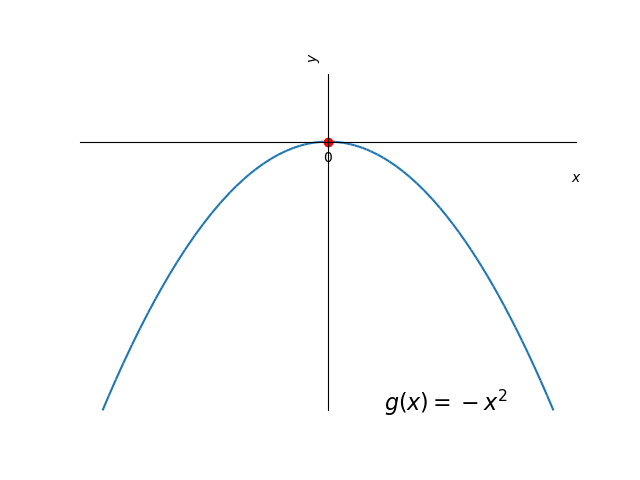
\includegraphics[width=0.32\textwidth]{./cap_apderiv/dados/fig_ex_vmaxminabs/fig_g}~
    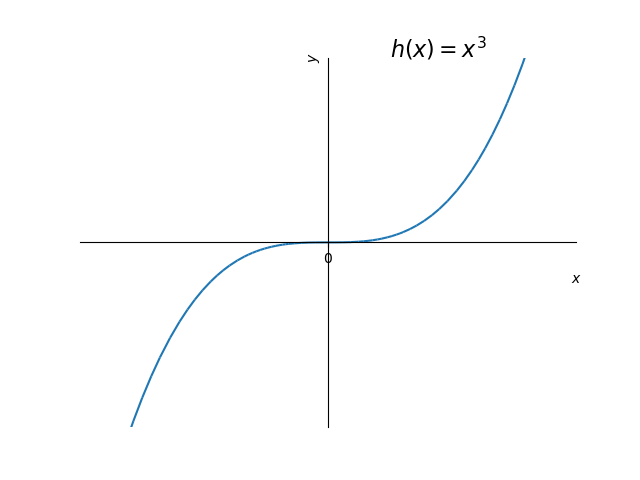
\includegraphics[width=0.32\textwidth]{./cap_apderiv/dados/fig_ex_vmaxminabs/fig_h}
    \caption{Esboço das funções discutidas no Exemplo \ref{ex:vmaxminabs}.}
    \label{fig:ex_vmaxminabs}
  \end{figure}
\end{ex}

\begin{teo}\normalfont{(Teorema do valor extremo\footnote{Este é uma versão do chamado \href{https://pt.wikipedia.org/wiki/Teorema_de_Weierstrass}{Teorema de Weierstrass}})}\label{teo:valorextremo}
  Se $f$ é uma função contínua em um intervalo fechado $[a, b]$, então $f$ assume tanto um valor máximo como um valor mínimo global em $[a, b]$.
\end{teo}
\begin{dem}
  A demonstração foge dos objetivos deste texto. Caso tenha interesse, consulte \cite{Avila1993a}.
\end{dem}

\begin{ex}\label{ex:fcont}
  Vejamos os seguintes casos:
  \begin{enumerate}[a)]
  \item  A função $\pmb{f(x) = (x-1)^2+1}$ é contínua no intervalo fechado $\displaystyle \left[0, \frac{3}{2}\right]$. Assume valor mínimo global $1$ no ponto $x=1$. Ainda, assume valor máximo global igual a $2$ no ponto $x=0$. Veja Figura \ref{fig:ex_fcont_f}.
  \begin{figure}[H]
    \centering
    \includegraphics[width=0.7\textwidth]{./cap_apderiv/dados/fig_ex_fcont/fig_f}
    \caption{Esboço do gráfico de $f(x) = (x-1)^2+1$ no intervalo $\displaystyle\left[0, \frac{3}{2}\right]$. Veja o Exemplo \ref{ex:fcont} a).}
    \label{fig:ex_fcont_f}
  \end{figure}
\item A função $\pmb{g(x) = \ln x}$ é contínua no intervalo $(0, e]$. Neste intervalo, assume valor máximo global no ponto $x=e$, mas não assume valor mínimo global. Veja Figura \ref{fig:ex_fcont_g}.
  \begin{figure}[H]
    \centering
    \includegraphics[width=0.7\textwidth]{./cap_apderiv/dados/fig_ex_fcont/fig_g}
    \caption{Esboço do gráfico de $g(x) = \ln x$ no intervalo $(0,e]$. Veja o Exemplo \ref{ex:fcont} b).}
    \label{fig:ex_fcont_g}
  \end{figure}
  
\item A função
  \begin{equation}
    h(x) = \left\{
      \begin{array}{ll}
        x &, 0\leq x < 1,\\
        0 &, x=1,
      \end{array}
\right.
\end{equation}
definida no intervalo $[0, 1]$ é descontínua no ponto $x=1$. Neste intervalo, assume valor mínimo global no ponto $x=0$, mas não assume valor máximo global. Veja a Figura \ref{fig:ex_fcont_h}.
  \begin{figure}[H]
    \centering
    \includegraphics[width=0.7\textwidth]{./cap_apderiv/dados/fig_ex_fcont/fig_h}
    \caption{Esboço do gráfico de $h(x)$ no intervalo $[0,1]$. Veja o Exemplo \ref{ex:fcont} c).}
    \label{fig:ex_fcont_h}
  \end{figure}
  \end{enumerate}
\end{ex}

Uma função $f$ tem um valor \emph{máximo local} em um ponto interior $x=a$ de seu domínio, se $f(x) < f(a)$ para todo $x$ em um intervalo aberto em torno de $a$, excluindo-se $x=a$. Analogamente, $f$ tem um valor \emph{mínimo local} em um ponto interior $x=b$ de seu domínio, se $f(x) > f(b)$  para todo $x$ em um intervalo aberto em torno de $b$, excluindo-se $x=b$. Em tais pontos, dizemos que a função têm valores \emph{extremos locais} (ou relativos). Um tal ponto é chamado de \emph{ponto de máximo local} ou \emph{de mínimo local}, conforme o caso.

\begin{ex}\label{ex:vmaxminloc}
  Consideremos a função
  \begin{equation}
    f(x) = \left\{
      \begin{array}{ll}
        -(x+1)^2-2 &, -2\leq x < -\frac{1}{2},\\
        |x| &, -\frac{1}{2} \leq x < 1,\\
        (x-2)^3+2 &, 1\leq x < 3.
      \end{array}
\right.
\end{equation}

  \begin{figure}[H]
    \centering
    \includegraphics[width=0.7\textwidth]{./cap_apderiv/dados/fig_ex_vmaxminloc/fig_f}
    \caption{Esboço do gráfico de $f(x)$ discutida no Exemplo \ref{ex:vmaxminloc}.}
    \label{fig:ex_vmaxminloc}
  \end{figure}
  
Na Figura \ref{fig:ex_vmaxminloc} temos o esboço de seu gráfico. Por inferência, temos que $f$ tem valores máximos locais nos pontos $x=-1$ e $x=-1/2$. No ponto $x=0$ tem um valor mínimo local. Observamos que $x=-2$, $x=2$ e $x=3$ não são pontos de extremos locais desta função. No ponto $x=-2$, $f$ tem seu valor mínimo global. Ainda, $f$ não tem valor máximo global.
\end{ex}

\begin{teo}\normalfont{(Teorema da derivada para pontos extremos locais.)}\label{teo:ptocritico}
  Se $f$ possui um valor extremo local em um ponto $x=a$ e $f$ é diferenciável neste ponto, então
  \begin{equation}
    f'(a) = 0.
  \end{equation}
\end{teo}
\begin{dem}
  Vamos considerar o caso em que $f$ possui um máximo local em $x=a$. Então, segue que
  \begin{gather}
    f'(a) = \lim_{h\to 0^+} \frac{f(x+h)-f(x)}{h} \leq 0\\
    f'(a) = \lim_{h\to 0^-} \frac{f(x+h)-f(x)}{h} \geq 0
  \end{gather}
  Logo, $f'(a) = 0$. Para o caso em que $f$ possui um mínimo local em $x=a$, consulte o Exercício \ref{exer:ptocritico}.
\end{dem}

Deste teorema, podemos concluir que uma função $f$ pode ter valores extremos em:
\begin{enumerate}[a)]
\item pontos interiores de seu domínio onde $f' = 0$,
\item pontos interiores de seu domínio onde $f'$ não existe, ou
\item pontos extremos de seu domínio.
\end{enumerate}

Um ponto interior do domínio de uma função $f$ onde $f'=0$ ou $f'$ não existe, é chamado de \emph{ponto crítico} da função.

\begin{obs}\label{obs:pt_critico_val_extremo}
  Uma função tem valores extremos em pontos críticos ou nos extremos de seu domínio.
\end{obs}


\begin{ex}
  Consideramos a função $f(x)$ discutida no Exemplo \ref{ex:vmaxminloc}. No ponto $x=-1$, $f'(-1)=0$ e $f$ tem valor máximo local neste ponto. Entretanto, no ponto $x=2$, também temos $f'(2)=0$, mas $f$ não tem valor extremo neste ponto.

  No ponto $x=0$, $f'(0)$ não existe e $f$ tem valor mínimo local neste ponto. No ponto, $x=-1/2$, $f'(1/2)$ não existe e $f$ tem valor máximo local neste ponto.

  Nos extremos do domínio, temos que $f$ tem valor mínimo global no ponto $x=-2$, mas não tem extremo global no ponto $x=3$.
\end{ex}

\subsection{Exercícios resolvidos}

% \begin{flushright}
%   [Vídeo] | [Áudio] | \href{https://phkonzen.github.io/notas/contato.html}{[Contatar]}
% \end{flushright}

\begin{exeresol}\label{exeresol:f_diff}
  Determine os pontos extremos da função $f(x) = (x+1)^2-1$ no intervalo $[-2,1]$.
\end{exeresol}
\begin{resol}
  Os valores extremos de um função podem ocorrer, somente, em seus pontos críticos ou nos extremos de seu domínio. Como $f(x) = (x+1)^2-1$ é diferenciável no intervalo $(-2,1)$, seus pontos críticos são pontos tais que $f'=0$. Para identificá-los, calculamos
  \begin{align}
    f'(x)=0 &\Rightarrow 2(x+1) = 0\\
            &\Rightarrow x = -1.
  \end{align}

  \begin{figure}[H]
    \centering
    \includegraphics[width=0.7\textwidth]{./cap_apderiv/dados/fig_exeresol_f_diff/fig_exeresol_f_diff}
    \caption{Esboço do gráfico da função $f(x) = (x+1)^2-1$ discutida no Exercício Resolvido \ref{exeresol:f_diff}.}
    \label{fig:exeresol_f_diff}
  \end{figure}

  Desta forma, $f$ pode ter valores extremos nos ponto $x=-2$, $x=-1$ e $x=1$. Analisamos, então, o esboço do gráfico da função (Figura \ref{fig:exeresol_f_diff}) e a seguinte tabela:\\
  \begin{center}
  \begin{tabular}[H]{l|ccc}
    $x$ & -2 & -1 & 1 \\\hline
    $f(x)$ & 0 & -1 & 3\\\hline
  \end{tabular}
\end{center}
Daí, podemos concluir que $f$ tem o valor mínimo global (e local) de $f(-1)=-1$ no ponto $x=-1$ e tem valor máximo global de $f(1)=3$ no ponto $x=1$.

\ifispython
Podemos usar o {\python}+{\sympy} para computar os pontos extremos e plotar a função. Por exemplo, com os seguintes comandos:
\begin{lstlisting}
import sympy as sp
x = sp.Symbol('x')
f = sp.lambdify(x, (x+1)**2-1)
# f' == 0
xc = sp.solve(sp.diff(f(x),x), x)
print(f"Pto. crítico xc = {xc}")
print(f"f(-2) = {f(-2)}")
print(f"f({xc[0]}) = {f(xc[0])}")
print(f"f(1) = {f(1)}")
sp.plot(f(x), (x,-2,1))
\end{lstlisting}
\fi
\end{resol}

\begin{exeresol}\label{exeresol:p_infl}
  Determine os pontos extremos da função $f(x)=x^3$ no intervalo $[-1, 1]$.
\end{exeresol}
\begin{resol}
  Como $f$ é diferenciável no intervalo $(-1, 1)$, temos que seus pontos críticos são tais que $f'(x)=0$. Neste caso, temos
  \begin{equation}
    3x^2=0\Rightarrow x=0
  \end{equation}
  é o único ponto crítico de $f$. Entretanto, analisando o gráfico desta função (Figura \ref{fig:exeresol_p_infl}) vemos que $f$ não tem valor extremo local neste ponto. Assim, seus pontos extremos só podem ocorrer nos extremos do domínio $[-1, 1]$. Concluímos que $f(-1)=-1$ é o valor mínimo global de $f$ e $f(1)=1$ é seu valor máximo global.

  \begin{figure}[H]
    \centering
    \includegraphics[width=0.7\textwidth]{./cap_apderiv/dados/fig_exeresol_p_infl/fig_exeresol_p_infl}
    \caption{Esboço do gráfico da função $f(x) = x^3$ discutida no Exercício Resolvido \ref{exeresol:p_infl}.}
    \label{fig:exeresol_p_infl}
  \end{figure}
\end{resol}

\subsection{Exercícios}

\begin{exer}
  Considere que uma dada função $f$ tenha o seguinte esboço de gráfico:

  \begin{center}
    \includegraphics[width=0.7\textwidth]{./cap_apderiv/dados/fig_exer_extfun/fig_exer_extfun}
  \end{center}

  Determine e classifique os pontos extremos desta função.
\end{exer}
\begin{resp}
  $x=-1$ ponto de mínimo global; $x=1$ ponto de máximo local; $x=2$ ponto de mínimo local; $x=\frac{5}{2}$ ponto de máximo global.
\end{resp}

\begin{exer}
  Dada a função $f(x)=x^2-2x+3$ restrita ao intervalo $[-1,2]$, determine:
  \begin{enumerate}[a)]
  \item seu(s) ponto(s) crítico(s).
  \item seu(s) ponto(s) extremo(s) e o(s) classifique.
  \item seu(s) valor(es) extremo(s) e o(s) classifique.
  \end{enumerate}
\end{exer}
\begin{resp}
  a)~$x=1$; b)~$x=-1$ ponto de máximo global; $x=1$ ponto de mínimo local e global; c)~$f(-1)=6$ valor máximo global; $f(1)=2$ valor mínimo local e global;
\end{resp}

\begin{exer}
  Dada a função $f(x)=-x^2+2x+1$ restrita ao intervalo $[0,3]$, determine:
  \begin{enumerate}[a)]
  \item seu(s) ponto(s) crítico(s).
  \item seu(s) ponto(s) extremo(s) e o(s) classifique.
  \item seu(s) valor(es) extremo(s) e o(s) classifique.
  \end{enumerate}
\end{exer}
\begin{resp}
  a)~$x=1$; b)~$x=1$ ponto de máximo local e global; $x=3$ ponto de mínimo global; c)~$f(1)=2$ valor máximo local e global; $f(3)=-2$ valor mínimo global;
\end{resp}

\begin{exer}
  Dada a função $f(x)=x^{3} - 3 x^{2} + 3 x$ restrita ao intervalo $[0, \infty)$, determine:
  \begin{enumerate}[a)]
  \item seu(s) ponto(s) crítico(s).
  \item seu(s) ponto(s) extremo(s) e o(s) classifique.
  \item seu(s) valor(es) extremo(s) e o(s) classifique.
  \end{enumerate}
\end{exer}
\begin{resp}
  a)~$x=1$; b)~$x=0$ ponto de mínimo global;c)~$f(0)=0$ valor mínimo global;
\end{resp}

\begin{exer}
  Dada a função $f(x)=x^{1/3}$ restrita ao intervalo $[-1,1]$, determine:
  \begin{enumerate}[a)]
  \item seu(s) ponto(s) crítico(s).
  \item seu(s) ponto(s) extremo(s) e o(s) classifique.
  \item seu(s) valor(es) extremo(s) e o(s) classifique.
  \end{enumerate}
\end{exer}
\begin{resp}
  a)~$x=0$; b)~$x=-1$ ponto de mínimo global; $x=1$ ponto de máximo global; c)~$f(-1)=-1$ valor mínimo global; $f(1)=1$ valor máximo global;
\end{resp}

\begin{exer}\label{exer:ptocritico}
  Mostre que se $f$ tem um mínimo local em $x=a$ e é diferenciável neste ponto, então $f'(a)=0$.
\end{exer}
\begin{resp}
  Dica: consulte a demonstração do Teorema \ref{teo:ptocritico}.
\end{resp}

\ifisbook
\subsubsection{Respostas}
\shipoutAnswer
\fi


\section{Teorema do valor médio}\label{cap_apderiv_sec_valormedio}

\begin{flushright}
  [Vídeo] | [Áudio] | \href{https://phkonzen.github.io/notas/contato.html}{[Contatar]}
\end{flushright}

O teorema do valor médio é uma aplicação do teorema de Rolle.

\subsection{Teorema de Rolle}

\begin{flushright}
  [Vídeo] | [Áudio] | \href{https://phkonzen.github.io/notas/contato.html}{[Contatar]}
\end{flushright}

O Teorema de Rolle fornece uma condição suficiente para que uma dada função diferenciável tenha derivada nula em pelo menos um ponto.

\begin{figure}[H]
  \centering
  \includegraphics[width=0.7\textwidth]{./cap_apderiv/dados/fig_teo_Rolle/fig_teo_Rolle}
  \caption{Ilustração do Teorema de Rolle.}
  \label{fig:teo_Rolle}
\end{figure}

\begin{teo}\normalfont{(Teorema de Rolle)}
  Seja $f$ uma função contínua no intervalo fechado $[a, b]$ e diferenciável no intervalo aberto $(a, b)$. Se
  \begin{equation}
    f(a)=f(b),
  \end{equation}
  então existe pelo menos um {\bf ponto crítico} $c\in (a, b)$ tal que
  \begin{equation}
    f'(c)=0.
  \end{equation}
\end{teo}
\begin{dem}
  A ideia da demonstração é uma consequência dos teoremas \ref{teo:valorextremo} e \ref{teo:ptocritico}. O primeiro, que existem pontos de mínimo e máximos globais  $m, M\in [a, b]$, i.e.
  \begin{equation}
    f(m) \leq f(x) \leq f(M).
  \end{equation}
  Se $m=M$, então $f$ é uma função contínua, donde segue que $f'(x)=0$ para todo $x\in (a, b)$. Agora, se $m\neq M$, então $m$ ou $M$ é um extremo local. Sem perda de generalidade, supomos que $c = m$ seja o mínimo local. Neste caso, o teorema \ref{teo:ptocritico} nos garante que $f'(c)=0$.
\end{dem}

\begin{ex}
  O polinômio $p(x) = x^3 - 4x^2 + 3x + 1$ tem pelo menos um ponto crítico no intervalo $(0,1)$ e no intervalo $(1,3)$. De fato,temos $p(0)=p(1)=1$ e, pelo teorema de Rolle, segue que existe pelo menos um ponto $c\in (0, 1)$ tal que $f'(c)=0$. Analogamente, como também $p(1)=p(3)=1$, segue do teorema que existe pelo menos um ponto crítico no intervalo $(1,3)$. Veja o esboço do gráfico de $p$ na Figura \ref{fig:ex_teo_Rolle}.

  \begin{figure}[H]
    \centering
    \includegraphics[width=0.7\textwidth]{./cap_apderiv/dados/fig_ex_teo_Rolle/fig_ex_teo_Rolle}
    \caption{Esboço do gráfico de $p(x) = x^3 - 4x^2 + 3x + 1$.}
    \label{fig:ex_teo_Rolle}
  \end{figure}
  
  De fato, como todo polinômio é derivável em toda parte, podemos calcular os pontos críticos como segue.
  \begin{align}
    p'(x) = 0 &\Rightarrow 3x^2 - 8x + 3 = 0 \\
              &\Rightarrow x = \frac{8 \pm \cancelto{2\sqrt{7}}{\sqrt{64 - 36}}}{6} \\
              &\Rightarrow x_1 = \frac{4 - \sqrt{7}}{3} \approx 0,45 \quad\text{ou}\quad x_2 = \frac{4 + \sqrt{7}}{3} \approx 2,22.
  \end{align}

  \ifispython
  Podemos usar os seguintes comandos\footnote{Veja a Observação \ref{obs:cap_apderiv_python}.} para computar os pontos críticos de $p$ e plotar seu gráfico:
\begin{verbatim}
>>> p = x**3 - 4*x**2 + 3*x + 1
>>> pc = solve(p.diff()); pc
[-sqrt(7)/3 + 4/3, sqrt(7)/3 + 4/3]
>>> plot(p,(x,-0.5,3.5))
\end{verbatim}
  \fi
\end{ex}

\begin{ex}\label{ex:nteo_Rolle}
  Vejamos os seguintes casos em que o Teorema de Rolle não se aplica:
  \begin{enumerate}[a)]
  \item A função
    \begin{equation}
      f(x) = \left\{
        \begin{array}{ll}
          x &, 0\leq x < 1,\\
          0 &, x=1.
        \end{array}
      \right.
    \end{equation}
    é tal que $f(0)=f(1)=0$, entretanto sua derivada $f'(x)=1$ no intervalo $(0, 1)$. Ou seja, a condição da $f$ ser contínua no intervalo fechado associado é necessária no teorema de Rolle. Veja a Figura \ref{fig:ex_fcont_h_2} para o esboço do gráfico desta função.
    
  \begin{figure}[H]
    \centering
    \includegraphics[width=0.7\textwidth]{./cap_apderiv/dados/fig_ex_fcont/fig_h}
    \caption{Esboço do gráfico da função referente ao Exemplo \ref{ex:nteo_Rolle} a).}
    \label{fig:ex_fcont_h_2}
  \end{figure}
  
\item Não existe ponto tal que a derivada da $g(x)=-|x-1|+1$ seja nula. Entretanto, notemos que $g(0)=g(2)=0$ e $g$ contínua no intervalo fechado $[0, 2]$. O teorema de Rolle não se aplica neste caso, pois $g$ não é derivável no intervalo $(0,2)$, mais especificamente, no ponto $x=1$. Veja a Figura \ref{fig:ex_nteo_Rolle_nderiv}.

  \begin{figure}[H]
    \centering
    \includegraphics[width=0.7\textwidth]{./cap_apderiv/dados/fig_ex_nteo_Rolle_nderiv/fig_ex_nteo_Rolle_nderiv}
    \caption{Esboço do gráfico da função referente ao Exemplo \ref{ex:nteo_Rolle} b).}
    \label{fig:ex_nteo_Rolle_nderiv}
  \end{figure}  
  \end{enumerate}
\end{ex}

\subsection{Teorema do valor médio}

\begin{flushright}
  [Vídeo] | [Áudio] | \href{https://phkonzen.github.io/notas/contato.html}{[Contatar]}
\end{flushright}

O teorema do valor médio é uma generalização do teorema de Rolle.

\begin{figure}[H]
  \centering
  \includegraphics[width=0.7\textwidth]{./cap_apderiv/dados/fig_teo_valmed/fig_teo_valmed}
  \caption{Ilustração do Teorema do valor médio.}
  \label{fig:teo_valor_medio}
\end{figure}

\begin{teo}\normalfont{(Teorema do valor médio\footnote{Também conhecido como Teorema de Lagrange.})}\label{teo:tvm}
  Seja $f$ uma função contínua no intervalo fechado $[a,b]$ e diferenciável no intervalo aberto $(a,b)$. Então, existe pelo menos um ponto $c\in (a,b)$ tal que
  \begin{equation}
    \frac{f(b)-f(a)}{b-a}=f'(c).
  \end{equation}
\end{teo}
\begin{dem}
  O resultado segue da aplicação do Teorema de Rolle \ref{teo:rolle} a seguinte função
  \begin{equation}
    F(x) = f(x) - f(a) - \frac{f(b) - f(a)}{b-a}(x-a)
  \end{equation}
  De fato, $F$ é contínua em $[a, b]$, diferenciável em $(a, b)$ e $F(a) = F(b)$. Logo, existe $c\in (a, b)$ tal que
  \begin{gather}
    F'(c) = 0\\
    f'(c) + \frac{f(b) - f(a)}{b-a} = 0\\
    \frac{f(b) - f(a)}{b-a} = f'(c)
  \end{gather}
\end{dem}

\begin{obs}
  Em um contexto de aplicação, o Teorema do valor médio relaciona a taxa de variação média da função em um intervalo $[a, b]$ com a taxa de variação instantânea da função em um ponto interior deste intervalo.
\end{obs}

\begin{ex}
  A função $f(x)=x^2$ é contínua no intervalo $[0,2]$ e diferenciável no intervalo $(0,2)$. Logo, segue do teorema do valor médio que existe pelo menos um ponto $c\in (0,2)$ tal que
  \begin{equation}
    f'(c)=\frac{f(2)-f(0)}{2-0}=2.
  \end{equation}
  De fato, $f'(x)=2x$ e, portanto, tomando $c=1$, temos $f'(c)=2$.
\end{ex}

\begin{corol}\normalfont{(Funções com derivadas nulas são constantes)}
  Se $f'(x)=0$ para todos os pontos em um intervalo $(a, b)$, então $f$ é constante neste intervalo.
\end{corol}
\begin{dem}
  De fato, sejam $x_1,x_2\in (a, b)$ e, sem perda de generalidade, $x_1<x_2$. Então, temos $f$ é contínua no intervalo $[x_1,x_2]$ e diferenciável em $(x_1,x_2)$. Segue do teorema do valor médio que existe $c\in (x_1,x_2)$ tal que
  \begin{equation}
    \frac{f(x_2)-f(x_1)}{x_2-x_1}=f'(c).
  \end{equation}
  Como $f'(c)=0$, temos $f(x_2)=f(x_1)$. Ou seja, a função vale sempre o mesmo valor para quaisquer dois pontos no intervalo $(a, b)$, logo é constante neste intervalo.
\end{dem}

\begin{corol}\normalfont{(Função com a mesma derivada diferem por uma constante)}\label{corol:apderiv_teomed_2}
  Se $f'(x)=g'(x)$ para todos os pontos em um intervalo aberto $(a,b)$, então $f(x)=g(x)+C$, $C$ constante, para todo $x\in (a,b)$.
\end{corol}
\begin{dem}
  Segue, imediatamente, da aplicação do corolário anterior à função $h(x)=f(x)-g(x)$.
\end{dem}

\begin{corol}\normalfont{(Monotonicidade e o sinal da derivada)}\label{corol:mono_deriv}
  Suponha que $f$ seja contínua em $[a,b]$ e derivável em $(a,b)$.
  \begin{enumerate}[a)]
  \item Se $f'(x)>0$ para todo $x\in (a,b)$, então $f$ é crescente\footnote{$f$ é função crescente em um intervalo $I$, quando $x_1>x_2$ em $I$ implica $f(x_1)>f(x_2)$.} em $[a,b]$.
  \item Se $f'(x)<0$ para todo $x\in (a,b)$, então $f$ é decrescente\footnote{$f$ é função decrescente em um intervalo $I$, quando $x_1>x_2$ em $I$ implica $f(x_1)<f(x_2)$.} em $[a,b]$.
  \end{enumerate}
\end{corol}
\begin{dem}
  Vamos demonstrar o item a), i.e. se $f'(x)>0$ para todo $x\in (a, b)$, então $f$ é crescente em $[a, b]$. Sejam $x_1<x_2$ com $x_1,x_2\in [a, b]$. Observamos que $f$ é contínua em $[x_1, x_2]$ e diferenciável em $(x_1, x_2)$. Logo, pelo Teorema do valor médio \ref{teo:tvm}, temos que existe $c\in (x_1, x_2)$ tal que
  \begin{equation}
    \frac{f(x_2)-f(x_1)}{x_2-x_1} = f'(c)
  \end{equation}
  ou, equivalentemente,
  \begin{equation}
    f(x_2)-f(x_1) = f'(c)\cdot(x_2-x_1).
  \end{equation}
  Como $f'(x)>0$ para todo $x\in (a, b)$ e $x_2-x_1>0$, concluímos que $f(x_2)-f(x_1)>0$, i.e.
  \begin{equation}
    f(x_1) < f(x_2).
  \end{equation}
  Com isso, mostramos que se $x_1<x_2$ com $x_1,x_2\in [a, b]$, então $f(x_1)<f(x_2)$, i.e. $f$ é crescente em $[a, b]$.

  A demonstração do item b) é análoga, consulte o Exercício \ref{exer:mono_deriv}.
\end{dem}

\begin{ex}
  Vamos estudar a monotonicidade da função polinomial $f(x) = x^3 - 4x^2 + 3x + 1$. Na Figura \ref{fig:ex_corol_mono_deriv}, temos o esboço de seu gráfico.
  
  \begin{figure}[H]
    \centering
    \includegraphics[width=0.7\textwidth]{./cap_apderiv/dados/fig_ex_corol_mono_deriv/fig_ex_corol_mono_deriv}
    \caption{Esboço do gráfico de $f(x) = x^3 - 4x^2 + 3x + 1$.}
    \label{fig:ex_corol_mono_deriv}
  \end{figure}

  Podemos usar o Corolário \ref{corol:mono_deriv} para estudarmos a monotonicidade (i.e. intervalos de crescimento ou decrescimento). Isto é, fazemos o estudo de sinal da derivada de $f$. Calculamos
  \begin{equation}
    f'(x) = 3x^2 - 8x + 3.
  \end{equation}
  Logo, temos
  \begin{center}
    \includegraphics[width=0.5\textwidth]{./cap_apderiv/dados/fig_ex_monoderiv_poli/fig_ex_monoderiv_poli}
  \end{center}
  Ou seja, $f'(x) < 0$ no conjunto $\displaystyle \left(-\infty, \frac{4-\sqrt{7}}{3}\right)\cup \left(\frac{4+\sqrt{7}}{3}, \infty\right)$ e $f'(x) < 0$ no conjunto $\displaystyle \left(\frac{4-\sqrt{7}}{3}, \frac{4+\sqrt{7}}{3}\right)$. Concluímos que $f$ é {\bf crescente} nos intervalos $\displaystyle \left(\left.-\infty, \frac{4-\sqrt{7}}{3}\right.\right]$ e $\displaystyle \left[\left.\frac{4+\sqrt{7}}{3}, \infty\right)\right.$, enquanto que $f$ é {\bf decrescente} no intervalo $\displaystyle \left[\frac{4-\sqrt{7}}{3}, \frac{4+\sqrt{7}}{3}\right]$.
\end{ex}

\begin{ex}
  A função exponencial $f(x) = e^x$ é crescente em toda parte. De fato, temos
  \begin{equation}
    f'(x) = e^x > 0,
  \end{equation}
  para todo $x\in\mathbb{R}$.
\end{ex}

\subsection{Exercícios resolvidos}

% \begin{flushright}
%   [Vídeo] | [Áudio] | \href{https://phkonzen.github.io/notas/contato.html}{[Contatar]}
% \end{flushright}

\begin{exeresol}
  Um carro percorreu 150 km em 1h30min. Mostre que em algum momento o carro estava a uma velocidade maior que 80 km/h.
\end{exeresol}
\begin{resol}
  Seja $s=s(t)$ a função distância percorrida pelo carro e $t$ o tempo, em horas, contado do início do percurso. Do teorema do valor médio, exite tempo $t_1\in (0,~1,5)$ tal que
  \begin{equation}
    f'(t_1) = \frac{s(1,5)-s(0)}{1,5-0} = \frac{150}{1,5} = 100~\text{km/h}.
  \end{equation}
  Ou seja, em algum momento o carro atingiu a velocidade de 100 km/h.
\end{resol}

\begin{exeresol}
  Estude a monotonicidade da função gaussiana $f(x) = e^{-x^2}$.  
\end{exeresol}
\begin{resol}
  Para estudarmos a monotonicidade de uma função, podemos fazer o estudo de sinal de sua derivada. Neste caso, temos
  \begin{equation}
    f'(x) = -2xe^{-x^2}.
  \end{equation}
  Assim, vemos que
  \begin{center}
    \includegraphics[width=0.5\textwidth]{./cap_apderiv/dados/fig_exeresol_gauss_estsinal/fig_exeresol_gauss_estsinal}
  \end{center}
  Concluímos que $f$ é crescente no intervalo $(-\infty, 0)$ e decrescente no intervalo $(0, \infty)$.
\end{resol}

\subsection{Exercícios}

\begin{exer}
  Estude a monotonicidade de $f(x) = x^2 - 2x$.
\end{exer}
\begin{resp}
  Decrescente: $(-\infty, 1]$; Crescente: $[1, \infty)$
\end{resp}

\begin{exer}
  Estude a monotonicidade de $\displaystyle f(x) = \frac{x^3}{3}-x$.
\end{exer}
\begin{resp}
  Decrescente: $[-1, 1]$; Crescente: $(-\infty, -1]$; $[1, \infty)$
\end{resp}

\begin{exer}
  Estude a monotonicidade de $\displaystyle f(x) = \ln x$.
\end{exer}
\begin{resp}
  Crescente: $(0, \infty)$
\end{resp}

\begin{exer}
  Estude a monotonicidade de $\displaystyle f(x) = xe^{-x}$.
\end{exer}
\begin{resp}
  Crescente: $(-\infty, 1)$; Decrescente de $(1, \infty)$
\end{resp}

\begin{exer}
  Demonstre que um polinômio cúbico pode ter no máximo $3$ raízes reais.
\end{exer}
\begin{resp}
  Dica: use o teorema de Rolle.
\end{resp}

\begin{exer}\label{exer:mono_deriv}
  Seja $f$ contínua em $[a,b]$ e derivável em $(a,b)$. Mostre que se $f'(x)<0$ para todo $x\in (a,b)$, então $f$ é decrescente em $[a, b]$. 
\end{exer}
\begin{resp}
  Dica: consulte a demonstração do item a) do Corolário \ref{corol:mono_deriv}.
\end{resp}

\ifisbook
\subsubsection{Respostas}
\shipoutAnswer
\fi


\section{Teste da primeira derivada}\label{cap_apderiv_sec_tder1}

\begin{flushright}
  [Vídeo] | [Áudio] | \href{https://phkonzen.github.io/notas/contato.html}{[Contatar]}
\end{flushright}

Na Seção \ref{cap_apderiv_sec_extfun}, vimos que os extremos de uma função ocorrem nos extremos de seu domínio ou em um ponto crítico. Aliado a isso, o Corolário \ref{corol:mono_deriv} nos fornece condições suficientes para classificar os pontos críticos como extremos locais.

Mais precisamente, seja $c$ um ponto crítico de uma função contínua $f$ e diferenciável em todos os pontos de um intervalo aberto $(a, b)$ contendo $c$, exceto possivelmente no ponto $c$. Movendo-se no sentido positivo em $x$:
\begin{itemize}
\item se $f'(x)$ muda de negativa para positiva em $c$, então $f$ possui um mínimo local em $c$;
\item se $f'(x)$ muda de positiva para negativa em $c$, então $f$ possui um máximo local em $c$;
\item se $f'$ não muda de sinal em $c$, então $c$ não é um extremo local de $f$.
\end{itemize}
Veja a Figura \ref{fig:tder1}.

\begin{figure}[H]
  \centering
  \includegraphics[width=0.7\textwidth]{./cap_apderiv/dados/fig_tder1/fig_tder1}
  \caption{Ilustração do teste da primeira derivada com $c$ ponto de máximo local e $d$ ponto de mínimo local.}
  \label{fig:tder1}
\end{figure}

\begin{ex}
  Consideremos a função $\displaystyle f(x)=\frac{x^3}{3}-2x^2+3x+3$. Como $f$ é diferenciável em toda parte, seus pontos críticos são aqueles tais que
  \begin{equation}
    f'(x)=0.
  \end{equation}
  Temos $f'(x) = x^2 - 4x + 3$. Segue, que os pontos críticos são
  \begin{align}
    x^2-4x+3=0 &\Rightarrow x = \frac{4\pm \cancelto{2}{\sqrt{16-12}}}{2} \\
    &\Rightarrow x_1 = 1,\quad x_2=3.
  \end{align}
  Com isso, temos
  \begin{center}
  \begin{tabular}{lccc}\hline
    Intervalo & $x<1$ & $1<x<3$ & $3<x$ \\\hline
    $f'$ & + & - & + \\
    $f$ & crescente & decrescente & crescente\\\hline
  \end{tabular}
\end{center}
  Então, do teste da primeira derivada, concluímos que $x_1=1$ é ponto de máximo local e que $x_2=3$ é ponto de mínimo local.

  \ifispython
  Podemos usar o \sympy~ para computarmos a derivada de $f$ com o comando\footnote{Veja a Observação \ref{obs:cap_apderiv_python}.}
\begin{verbatim}
fl = diff(x**3/3-2*x**2+3*x+3)
\end{verbatim}
  Então, podemos resolver $f'(x)=0$ com o comando
\begin{verbatim}
solve(fl)
\end{verbatim}
  e, por fim, podemos fazer o estudo de sinal da $f'$ com os comandos
\begin{verbatim}
reduce_inequalities(fl<0)
reduce_inequalities(fl>0)
\end{verbatim}
  \fi
\end{ex}

\subsection{Exercícios resolvidos}

% \begin{flushright}
%   [Vídeo] | [Áudio] | \href{https://phkonzen.github.io/notas/contato.html}{[Contatar]}
% \end{flushright}

\begin{exeresol}
  Determine e classifique os extremos da função
  \begin{equation}
    f(x) = x^4 - 4x^3 + 4x^2.
  \end{equation}
\end{exeresol}
\begin{resol}
  Como o domínio da $f$ é $(-\infty, \infty)$ e $f$ é diferenciável em toda parte, temos que seus extremos ocorrem em pontos críticos tais que
  \begin{equation}
    f'(x)=0.
  \end{equation}
  Resolvendo, obtemos
  \begin{align}
    4x^3-12x^2+8x=0 &\Rightarrow 4x(x^2-3x+2)=0
  \end{align}
  Logo,
  \begin{align}
    4x=0 \quad\text{ou}\quad &x^2-3x+2=0\\
    x_1 = 0                  &x = \frac{3\pm 1}{2}. \\
                             &x_2 = 1,\quad x_3=2
  \end{align}
  Portanto, os ponto críticos são $x_1=0$, $x_2=1$ e $x_3=2$. Fazendo o estudo de sinal da $f'$, temos
  \begin{center}
    \begin{tabular}{lcccc}\hline
                 & $x<0$ & $0<x<1$ & $1<x<2$ & $2<x$ \\\hline
      $4x$       & -       &     +       &     +      &   +  \\
      $x^2-3x+2$ & +       &     +       &     -      &   +   \\
      $f'(x)$    & -       &     +       &     -      &   +   \\
      $f$        & decrescente & crescente & decrescente & crescente \\\hline
    \end{tabular}\\
  \end{center}
  Então, do teste da primeira derivada, concluímos que $x_1=0$ é ponto de mínimo local, $x_2=-2$ é ponto de máximo local e $x_3=-1$ é ponto de mínimo local.

  \ifispython
  Podemos usar os seguintes comandos do \sympy\footnote{Veja a Observação \ref{obs:cap_apderiv_python}.} para resolvermos este exercício:
\begin{verbatim}
# f'
fl = Lambda(x, diff(x**4 - 4*x**3 + 4*x**2,x))
# f'(x) = 0
solve(fl(x))
# fl(x) < 0
reduce_inequalities(fl(x)<0)
# fl(x) > 0
reduce_inequalities(fl(x)>0)
\end{verbatim}
  \fi
\end{resol}

\begin{exeresol}
  Encontre o valor máximo global de $f(x) = (x-1)e^{-x}$.
\end{exeresol}
\begin{resol}
  Como $f$ é diferenciável em toda parte, temos que seu máximo ocorre em ponto crítico tal que
  \begin{align}
    f'(x) = 0 &\Rightarrow (2-x)e^{-x} = 0 \\
              &\Rightarrow 2-x = 0 \\
              &\Rightarrow x = 2.
  \end{align}
  Fazendo o estudo de sinal da derivada, obtemos
  \begin{center}
    \begin{tabular}[H]{lcc}
         & x<0 & 0<x \\\hline
      f' & + & - \\
      f  & crescente & decrescente \\\hline
    \end{tabular}
  \end{center}
  Portanto, do teste da primeira derivada, podemos concluir que $x=2$ é ponto de máximo local. O favor da função neste ponto é $f(2) = e^{-2}$. Ainda, temos
  \begin{align}
    &\lim_{x\to -\infty} (x-1)e^{-x} = -\infty, \\
    &\lim_{x\to \infty} (x-1)e^{-x} = 0.
  \end{align}
  Por tudo isso, concluímos que o valor máximo global de $f$ é $f(2) = e^{-2}$.

  \ifispython
  Podemos usar os seguintes comandos do \sympy\footnote{Veja a Observação \ref{obs:cap_apderiv_python}.} para resolvermos este exercício:
\begin{verbatim}
# f(x)
f = Lambda(x, (x-1)*exp(-x))
# f'(x)
fl = Lambda(x, diff(f(x),x))
# pontos críticos
xc = solve(fl(x))
# f'(x) < 0
reduce_inequalities(fl(x)<0)
# f'(x) > 0
reduce_inequalities(fl(x)>0)
# lim f(x), x->-oo
limit(f(x),x,-oo)
# lim f(x), x->oo
limit(f(x),x,oo)
# f(2)
f(xc[0])
\end{verbatim}
  \fi
\end{resol}

% \begin{exer}\label{exeresol:ap}
%   Um terreno retangular deve ser cercado usando cercas diferentes. Em dois lados opostos deve ser aplicada uma cerca mais resistente que custa \$ 2 o metro, nos outros dois lados deve ser aplicada uma cerca que custa apenas \$ 1 o metro. Quais as dimensões da maior área que pode ser cercada a um custo total de \$ 4000.  
% \end{exer}
% \begin{resol}
%   Denotando por $x$ a largura e por $y$ o comprimento do retângulo, temos que sua área é dada por
%   \begin{equation}
%     A = xy
%   \end{equation}
%   Também, temos que a restrição do custo total nos fornece
%   \begin{equation}
%     2x
%   \end{equation}
% \end{resol}

\subsection{Exercícios}

\begin{exer}
  Use o teste da primeira derivada para encontrar e classificar o(s) ponto(s) extremo(s) de $f(x) = x^2 - 2x$.
\end{exer}
\begin{resp}
  $x=1$ ponto de mínimo global
\end{resp}

\begin{exer}
    Use o teste da primeira derivada para encontrar e classificar o(s) ponto(s) extremo(s) de $\displaystyle f(x) = \frac{x^3}{3}-x$.
\end{exer}
\begin{resp}
  $x_1=-1$ ponto de máximo local; $x_2=1$ ponto de mínimo local;
\end{resp}

\begin{exer}
  Use o teste da primeira derivada para encontrar e classificar o(s) ponto(s) extremo(s) de $\displaystyle f(x) = x^{2/3}(x-1)$.
\end{exer}
\begin{resp}
  $x_1=0$ ponto de máximo local; $x_2=2/5$ ponto de mínimo local;
\end{resp}

\ifisbook
\subsubsection{Respostas}
\shipoutAnswer
\fi


\section{Concavidade e o Teste da segunda derivada}\label{cap_apderiv_sec_tder2}

\begin{flushright}
  [Vídeo] | [Áudio] | \href{https://phkonzen.github.io/notas/contato.html}{[Contatar]}
\end{flushright}

O gráfico de uma função diferenciável $f$ é
\begin{enumerate}[a)]
\item {\bf côncavo para cima} em um intervalo aberto $I$, se $f'$ é crescente em $I$;
\item {\bf côncavo para baixo} em um intervalo aberto $I$, se $f'$ é decrescente em $I$.
\end{enumerate}

Assumindo que $f$ é duas vezes diferenciável, temos que a monotonicidade de $f'$ está relacionada ao sinal de $f''$ (a segunda derivada de $f$). Logo, o gráfico de $f$ é
\begin{enumerate}[a)]
\item {\bf côncavo para cima} em um intervalo aberto $I$, se $f'' > 0$ em $I$;
\item {\bf côncavo para baixo} em um intervalo aberto $I$, se $f'' < 0$ em $I$.
\end{enumerate}

\begin{ex}
  Vejamos os seguintes casos:
  \begin{enumerate}[a)]
  \item o gráfico de $f(x) = x^2$ é uma parábola côncava para cima em toda parte. De fato, temos
    \begin{equation}
      f'(x) = 2x,
    \end{equation}
    uma função crescente em toda parte. Também, temos
    \begin{equation}
      f''(x) = 2 > 0,
    \end{equation}
    em toda parte.
  \item o gráfico de $g(x) = -x^2$ é uma parábola côncava para baixo em toda parte. De fato, temos
    \begin{equation}
      g'(x) = -2x,
    \end{equation}
    uma função decrescente em toda parte. Também, temos
    \begin{equation}
      g''(x) = -2 < 0,
    \end{equation}
    em toda parte.
  \item o gráfico da função $h(x) = x^3$ é côncavo para baixo em $(-\infty, 0)$ e côncavo para cima em $(0, \infty)$. De fato, temos
    \begin{equation}
      h'(x) = x^2,
    \end{equation}
    que é uma função decrescente em $(-\infty, 0]$ e crescente em $[0, \infty)$. Também, temos
    \begin{equation}
      h''(x) = 2x
    \end{equation}
    que assume valores negativos em $(-\infty, 0)$ e valores positivos em $(0, \infty)$.
  \end{enumerate}
\end{ex}

Um ponto em que o gráfico de uma função $f$ muda de concavidade é chamado de {\bf ponto de inflexão}. Em tais pontos temos
\begin{equation}
  f'' = 0\quad\text{ou}\quad\nexists f''.
\end{equation}

\begin{ex}
  Vejamos os seguintes casos:
  \begin{enumerate}[a)]
  \item O gráfico da função $f(x) = x^3$ tem $x=0$ como único ponto de inflexão. De fato, temos
    \begin{equation}
      f'(x) = 3x^2
    \end{equation}
    que é diferenciável em toda parte com
    \begin{equation}
      f''(x) = 6x.
    \end{equation}
    Logo, os pontos de inflexão ocorrem quando
    \begin{align}
      f''(x) = 0 &\Rightarrow 6x = 0 \\
                 &\Rightarrow x = 0.
    \end{align}
  \item O gráfico da função $g(x) = \sqrt[3]{x}$ tem $x=0$ como único ponto de inflexão. De fato, temos
    \begin{equation}
      g'(x) = \frac{1}{3}x^{-\frac{2}{3}},\quad x\neq 0.
    \end{equation}
    Segue que
    \begin{equation}
      g''(x) = -\frac{2}{9}x^{-\frac{5}{3}},\quad x\neq 0,
    \end{equation}
    donde $g'' > 0$ em $(-\infty, 0)$e $g'' < 0$ em $(0, \infty)$. Isto é, o gráfico de $g$ muda de concavidade em $x=0$, $\nexists g''(0)$, sendo $g$ côncava para cima em $(-\infty, 0)$ e côncava para baixo em $(0, \infty)$.
\end{enumerate}
\end{ex}

\subsection{Teste da segunda derivada}

\begin{flushright}
  [Vídeo] | [Áudio] | \href{https://phkonzen.github.io/notas/contato.html}{[Contatar]}
\end{flushright}

Seja $x=x_0$ um ponto crítico de uma dada função $f$ duas vezes diferenciável e $f''$ contínua em um intervalo aberto contendo $x=x_0$. Temos
\begin{enumerate}[a)]
\item se $f'(x_0) = 0$ e $f''(x_0) > 0$, então $x=x_0$ é um ponto de mínimo local de $f$;
\item se $f'(x_0) = 0$ e $f''(x_0) < 0$, então $x=x_0$ é um ponto de máximo local de $f$.
\end{enumerate}

\begin{ex}
  A função $f(x) = 2x^3 - 9x^2 + 12x - 2$ tem pontos críticos
  \begin{align}
    f'(x) = 6x^2 - 18x + 12 = 0 &\Rightarrow x^2 - 3x + 2 = 0 \\
                                &\Rightarrow x = \frac{3 \pm \sqrt{1}}{2}\\
                                &\Rightarrow x_1 = 1,\quad x_2 = 2.
  \end{align}
  A segunda derivada de $f$ é
  \begin{equation}
    f''(x) = 12x - 18.
  \end{equation}
  Logo, como $f''(x_1) = f''(1) = -6 < 0$, temos que $x_1 = 1$ é ponto de máximo local de $f$. E, como $f''(x_2) = f''(2) = 6 > 0$, temos que $x_2 = 2$ é ponto de mínimo local de $f$.
\end{ex}

\begin{obs}
  Se $f'(x_0) = 0$ e $f''(x_0) = 0$, então $x=x_0$ pode ser ponto extremo local de $f$ ou não. Ou seja, o teste é inconclusivo.
\end{obs}

\begin{ex}
  Vejamos os seguintes casos:
  \begin{enumerate}[a)]
  \item A função $f(x) = x^3$ tem ponto crítico
    \begin{align}
      f'(x) = 0 &\Rightarrow 3x^2 = 0 \\
                &\Rightarrow x = 0.
    \end{align}
    Neste ponto, temos
    \begin{equation}
      f''(x) = 6x \Rightarrow f''(0) = 0.
    \end{equation}
    Neste caso, $x=0$ não é ponto de extremo local e temos $f'(0) = 0$ e $f''(0) = 0$.
  \item A função $f(x) = x^4$ tem um ponto crítico
    \begin{align}
      f'(x) = 0 &\Rightarrow 4x^3 = 0 \\
                &\Rightarrow x = 0.
    \end{align}
    Neste ponto, temos
    \begin{equation}
      f''(x) = 12x^2 \Rightarrow f''(0) = 0.
    \end{equation}
    Neste caso, $x=0$ é ponto de mínimo local e temos $f'(0)=0$ e $f''(0) = 0$.
  \end{enumerate}
\end{ex}

\subsection{Exercícios resolvidos}

% \begin{flushright}
%   [Vídeo] | [Áudio] | \href{https://phkonzen.github.io/notas/contato.html}{[Contatar]}
% \end{flushright}

\begin{exeresol}
  Encontre o valor máximo global de $f(x) = (x-1)e^{-x}$.
\end{exeresol}
\begin{resol}
  Como $f$ é diferenciável em toda parte, temos que seu valor máximo (se existir) ocorre em ponto crítico tal que
  \begin{align}
    f'(x) = 0 &\Rightarrow (2-x)e^{-x} = 0 \\
              &\Rightarrow 2-x = 0 \\
              &\Rightarrow x = 2.
  \end{align}
  Agora, usando o teste da segunda derivada, temos
  \begin{align}
    f''(x) = (x-3)e^{-x} \Rightarrow f''(2) = -e^{-2} < 0.
  \end{align}
  Logo, $x=2$ é ponto de máximo local. O favor da função neste ponto é $f(2) = e^{-2}$. Ainda, temos
  \begin{align}
    &\lim_{x\to -\infty} (x-1)e^{-x} = -\infty, \\
    &\lim_{x\to \infty} (x-1)e^{-x} = 0.
  \end{align}
  Por tudo isso, concluímos que o valor máximo global de $f$ é $f(2) = e^{-2}$.

  \ifispython
  Podemos usar os seguintes comandos do \sympy\footnote{Veja a Observação \ref{obs:cap_apderiv_python}.} para resolvermos este exercício:
\begin{verbatim}
>>> f = (x-1)*exp(-x)
>>> fl = diff(f,x)
>>> f = Lambda(x, (x-1)*exp(-x))
>>> fl = Lambda(x, diff(f(x),x))
>>> solve(fl(x))
[2]
>>> fll = Lambda(x, diff(f(x),x,2))
>>> fll(2)
  -2
-e  
>>> f(2), fl(2), fll(2)
 -2       -2
e  , 0, -e  
>>> limit(f(x),x,oo)
0
>>> limit(f(x),x,-oo)
-oo
\end{verbatim}
  \fi
\end{resol}

\begin{exeresol}
  Determine e classifique os extremos da função
  \begin{equation}
    f(x) = x^4 - 4x^3 + 4x^2
  \end{equation}
  restrita ao intervalo de $[-1, 3]$.
\end{exeresol}
\begin{resol}
  Como $f$ é diferenciável em $(-1, 3)$, temos que seus extremos locais ocorrem nos seguintes pontos críticos
  \begin{align}
    f'(x) = 0 &\Rightarrow 4x^3-12x^2+8x = 0 \\
              &\Rightarrow 4x(x^2-3x+2)=0 \\
              &\Rightarrow x_1 = 0, x_2 = 1, x_3 = 2.
  \end{align}
  Calculando a segunda derivada de $f$, temos
  \begin{equation}
    f''(x) = 12x^2 - 24x + 8.
  \end{equation}
  Do teste da segunda derivada, temos
  \begin{align}
    & f''(x_1) = f''(0) = 8 > 0 \Rightarrow x_1=0 ~ \text{pto. mín. local} \\
    & f''(x_2) = f''(1) = -4 < 0 \Rightarrow x_2=1 ~ \text{pto. máx. local} \\
    & f''(x_3) = f''(2) = 8 > 0 \Rightarrow x_3=2 ~ \text{pto. mín. local} 
  \end{align}
  Agora, vejamos os valores de $f$ em cada ponto de interesse.
  \begin{center}
    \begin{tabular}{l|ccccc}
      $x$     & $-1$ & $0$ & $1$ & $2$ & $3$ \\\hline
      $f(x)$  & $9$    & $0$   & $1$   & $0$ & $9$ \\
    \end{tabular}\\
  \end{center}
  Então, podemos concluir que $x=-1$ e $x=3$ são pontos de máximo global (o valor máximo global é $f(-1)=f(3)=9$), $x=1$ é ponto de máximo local, $x=0$ e $x=2$ são pontos de mínimo global (o valor mínimo global é $f(0)=f(2)=0$).
  
  \ifispython
  Podemos usar os seguintes comandos do \sympy\footnote{Veja a Observação \ref{obs:cap_apderiv_python}.} para resolvermos este exercício:
\begin{verbatim}
>>> f = Lambda(x, x**4 - 4*x**3 + 4*x**2)
>>> fl = Lambda(x, diff(f(x),x))
>>> solve(fl(x))
[0, 1, 2]
>>> fll = Lambda(x, diff(fl(x),x))
>>> fll(0), fll(1), fll(2)
(8, -4, 8)
>>> f(-1), f(0), f(1), f(2), f(3)
(9, 0, 1, 0, 9)
\end{verbatim}
  \fi
\end{resol}

\subsection{Exercícios}

\begin{exer}
  Use o teste da segunda derivada para encontrar e classificar o(s) ponto(s) extremo(s) de $f(x) = x^2 - 2x$.
\end{exer}
\begin{resp}
  $x=1$ ponto de mínimo global
\end{resp}

\begin{exer}
  Use o teste da segunda derivada para encontrar e classificar o(s) ponto(s) extremo(s) de $\displaystyle f(x) = \frac{x^3}{3}-x$.
\end{exer}
\begin{resp}
  $x_1=-1$ ponto de máximo local; $x_2=1$ ponto de mínimo local;
\end{resp}

\begin{exer}
  Use o teste da segunda derivada para encontrar e classificar o(s) ponto(s) extremo(s) de $\displaystyle f(x) = x^{2/3}(x-1)$.
\end{exer}
\begin{resp}
  $x_1=0$ ponto de máximo local; $x_2=2/5$ ponto de mínimo local;
\end{resp}

\begin{exer}
  Seja $f(x) = -x^4$. Mostre que $x=0$ é ponto de máximo local de $f$ e que $f'(0) = f''(0) = 0$.
\end{exer}
\begin{resp}
  $f'(x) = -4x^3$, $f'(0)=0$. Pelo teste da 1. derivada, temos que $x=0$ é ponto de máximo local. $f''(x) = -12x^2$, $f''(0)=0$.
\end{resp}

\ifisbook
\subsubsection{Respostas}
\shipoutAnswer
\fi

\chapter{Integração}\label{cap_int}
\thispagestyle{fancy}

\section{Noção de integral}\label{cap_int_sec_nocaoint}

\subsection{Soma de Riemann}

Seja \hl{$f$ uma função contínua definida em um intervalo fechado $[a, b]$}. Seja, também, \hl{$P$} a seguinte \hl{\emph{partição} de $[a, b]$}
\begin{equation}
  P = \{a=x_0<x_1<x_2<\cdots<x_n=b\},
\end{equation}
onde $n+1$ é o número de pontos na partição. Definimos
\begin{equation}
  \hleq\Delta x_i = x_{i} - x_{i-1}
\end{equation}
o \hl{tamanho de cada subintervalo $I_{i} = [x_{i-1}, x_{i}]$ da partição}, com $i = 1, 2, \cdots, n$. A \hl{\emph{norma da partição}} é definida por
\begin{equation}
  \hleq\|P\| := \max_{i=1, \dotsc, n} \Delta x_i,
\end{equation}
i.e. \hl{o tamanho do maior subintervalo da partição}. Com isso, chama-se de uma \hl{\emph{soma de Riemann}}{\riemann} toda a expressão da forma
\begin{equation}\hleq
  S_n := \sum_{i=1}^n f(x_i^*)\Delta x_i,
\end{equation}
onde \hl{$x_i^*\in [x_i, x_{i-1}]$ (arbitrariamente escolhido)}. Consulte a Figura \ref{fig:soma_de_Riemann}.

\begin{figure}[H]
  \centering
  \includegraphics[width=0.9\textwidth]{./cap_int/dados/fig_soma_de_Riemann/fig_soma_de_Riemann}
  \caption{Ilustração da soma de Riemann.}
  \label{fig:soma_de_Riemann}
\end{figure}

\hl{No caso de uma função não negativa, uma soma de Riemann é uma aproximação da área sob seu gráfico e o eixo das abscissas}\footnote{Consulte o Exercício \ref{exer:int_geoRiemann} para uma interpretação geométrica no caso geral de funções contínuas.}. 

\subsection{Integral}

\hl{A integral (definida) de $a$ até $b$ de uma dada função $f$ em relação a $x$ é} denotada e definida por
\begin{equation}\hleq
  \int_a^b f(x)\,dx := \lim_{\|P\|\to 0} \sum_{i=1}^n f(x_i^*)\Delta x_i.
\end{equation}
De forma genérica, \hl{a integral definida de $a$ até $b$ é o limite das somas de Riemann quando a norma das partições $P$ do intervalo $[a, b]$ tendem a zero. Quando o limite existe, dizemos que $f$ é \emph{integrável} no intervalo $[a, b]$}.

Na notação de integral definida acima, chamamos $a$ de \hl{\emph{limite inferior}} e $b$ de \hl{\emph{limite superior de integração}}, $f$ é chamada de \hl{\emph{integrando}} e $x$ de \hl{\emph{variável de integração}}.

\begin{obs}
  Funções contínuas são funções integráveis.
\end{obs}

\begin{figure}[H]
  \centering
  \includegraphics[width=0.9\textwidth]{./cap_int/dados/fig_geointdef/fig_geointdef}
  \caption{A integral definida como a área sob o gráfico.}
  \label{fig:geointdef}
\end{figure}

\begin{obs}\normalfont{(Área sob o gráfico)}\label{obs:int_area}
  No caso de uma função não negativa,
  \begin{equation}\hleq
    \int_a^b f(x)\,dx
  \end{equation}
  \hl{é a área sob o gráfico de $f$}\footnote{Consulte o Exercício \ref{exer:int_geointdef} para uma interpretação geométrica no caso geral de funções contínuas.}. Consulte a Figura \ref{fig:geointdef}.  
\end{obs}

\begin{ex}
  Vamos calcular
  \begin{equation}
    \int_0^1 1\,dx.
  \end{equation}
  Aqui, o integrando é a função constante $f(x) \equiv 1$ e o \emph{intervalo de integração} é $[a, b]$. Da Observação \ref{obs:int_area}, temos que esta integral é a área sob o gráfico de $f$ no intervalo $[0, 1]$. Esta área é um retângulo de altura $1$ e comprimento $1$. Logo,
  \begin{equation}
    \int_0^1 1\,dx = 1\cdot 1 = 1.
  \end{equation}

\begin{lstlisting}
import sympy as sym
from sympy.abc import x
sym.integrate(1, (x, 0, 1))
\end{lstlisting}

\begin{verbatim}
1
\end{verbatim}

\end{ex}

\subsection{Exercícios resolvidos}

\begin{exeresol}
  Calcule
  \begin{equation}
    \int_{-1}^1 \sqrt{1 - x^2}\,dx.
  \end{equation}
\end{exeresol}
\begin{resol}
  Esta integral corresponde à área sob o gráfico da função $f(x) = \sqrt{1 - x^2}$ restrita ao intervalo $[-1, 1]$. Observando que
  \begin{align}
    y = \sqrt{x^2 - 1} &\Rightarrow y^2 = 1 - x^2\\
                       &\Rightarrow y^2 + x^2 = 1,
  \end{align}
  vemos que esta é a área do semicírculo de raio $1$. Logo,
  \begin{equation}
    \int_{-1}^1 \sqrt{1 - x^2}\,dx = \frac{\pi \cdot 1^2}{2} = \frac{\pi}{2}.
  \end{equation}

\begin{lstlisting}
import sympy as sym
from sympy.abc import x
sym.integrate(sym.sqrt(1-x**2), (x, -1, 1))
\end{lstlisting}

\begin{verbatim}
pi/2
\end{verbatim}

\end{resol}

\begin{exeresol}
  Determine a função $F(x)$ tal que
  \begin{equation}
    F(x) = \int_0^x t\,dt,
  \end{equation}
  para todo $x\geq 0$. Então, mostre que $F'(x) = x$.
\end{exeresol}
\begin{resol}
  A integral definida
  \begin{equation}
    \int_0^x t\,dt
  \end{equation}
  é a área sob o gráfico de $f(t) = t$ restrita no intervalo $[0, x]$. Isto é, a área do triângulo retângulo de base $x$ e altura $x$. Logo,
  \begin{equation}
    F(x) = \int_0^x t\,dt = \frac{x\cdot x}{2} = \frac{x^2}{2}.
  \end{equation}
  Ou seja, temos $F(x) = x^2/2$ e, portanto,
  \begin{equation}
    F'(x) = \frac{1}{2}\cdot 2x = x.
  \end{equation}

\begin{lstlisting}
import sympy as sym
from sympy.abc import x,t
F = sym.integrate(t, (t, 0, x))
print('F(x) =', F)
\end{lstlisting}

\begin{verbatim}
F(x) = x**2/2  
\end{verbatim}

\begin{lstlisting}
sym.diff(F, x)
\end{lstlisting}

\begin{verbatim}
x
\end{verbatim}

\end{resol}

\subsection{Exercícios}

\begin{exer}
  Calcule
  \begin{equation}
    \int_{-1}^2 2\,dx.
  \end{equation}
\end{exer}
\begin{resp}
  $6$
\end{resp}

\begin{exer}
  Calcule
  \begin{equation}
    \int_{-3}^{-1} 1-x\,dx.
  \end{equation}
\end{exer}
\begin{resp}
  $6$
\end{resp}

\begin{exer}
  Determine $F(x)$ tal que
  \begin{equation}
    F(x) = \int_{0}^{x} t+1\,dt.
  \end{equation}
  para $x\geq 0$. Então, calcule $F'(x)$.
\end{exer}
\begin{resp}
  $\displaystyle F(x) = \frac{x^2}{2} + x$; $F'(x) = x + 1$.
\end{resp}

\begin{exer}\label{exer:int_geoRiemann}
  Faça uma interpretação geométrica da uma soma de Riemann aplicada a uma função contínua e não positiva. Estenda sua interpretação para funções contínuas arbitrárias.
\end{exer}
\begin{resp}
  Dica: a soma de Riemann é uma aproximação da área líquida sob o gráfico da função.
\end{resp}

\begin{exer}\label{exer:int_geointdef}
  Faça uma interpretação geométrica de
  \begin{equation}
    \int_a^b f(x)\,dx
  \end{equation}
  quando $f$ é uma função contínua e não positiva. Estenda sua interpretação para funções contínuas arbitrárias.
\end{exer}
\begin{resp}
  Dica: $\displaystyle \int_a^b f(x)\,dx$é a área líquida sob o gráfico da função.
\end{resp}

\begin{exer}
  Calcule
  \begin{equation}
    \int_{-1}^2 -1\,dx.
  \end{equation}
\end{exer}
\begin{resp}
  $-3$
\end{resp}

\begin{exer}
  Calcule
  \begin{equation}
    \int_{-1}^{1} x\,dx.
  \end{equation}
\end{exer}
\begin{resp}
  $0$
\end{resp}

\ifisbook
\subsubsection{Respostas}
\shipoutAnswer
\fi


\section{Propriedades de integração}\label{cap_int_sec_propint}

\begin{flushright}
  [Vídeo] | [Áudio] | \href{https://phkonzen.github.io/notas/contato.html}{[Contatar]}
\end{flushright}

Na Seção \ref{cap_int_sec_nocaoint}, vimos que \hl{a integral definida de uma dada função $f$ em um intervalo $[a, b]$ está associada à área (líquida) entre seu gráfico e as retas $y=0$, $x=a$ e $x=b$}. Veja a Figura \ref{fig:geointdef}.

Com base nesta noção geométrica, podemos inferir as seguintes propriedades de integração para funções integráveis $f$ e $g$:
\begin{enumerate}[a)]
\item \hl{\emph{Integral degenerada}}
  \begin{equation}\hleq
    \int_a^a f(x)\,dx = 0
  \end{equation}
\item \hl{\emph{Multiplicação por escalar}}
  \begin{equation}\hleq
    \int_a^b k\cdot f(x)\,dx = k\cdot\int_a^b f(x)\,dx
  \end{equation}
\item \hl{\emph{Soma/subtração}}
  \begin{equation}\hleq
    \int_a^b \left[f(x)\pm g(x)\right]\,dx = \int_a^b f(x)\,dx \pm \int_a^b g(x)\,dx
  \end{equation}
\item \hl{\emph{Sobreposição/concatenação de intervalos}}
  \begin{equation}\hleq
    \int_a^b f(x)\,dx = \int_a^c f(x)\,dx + \int_c^b f(x)\,dx
  \end{equation}
\item \hl{\emph{Cotas inferior e superior}}
  \begin{equation}\hleq
    \min_{x\in [a, b]} \{f(x)\}\cdot (b-a) \leq \int_a^b f(x)\,dx \leq \max_{x\in [a, b]} \{f(x)\}\cdot (b-a)
  \end{equation}
\end{enumerate}

\begin{ex}
  Sejam $f$ e $g$ funções integráveis tais que
  \begin{gather}
    \int_{-1}^4 f(x)\,dx = 2,\\
    \int_4^5 f(x)\,dx = 3,\\
    \int_{-1}^4 g(x)\,dx = -1.
  \end{gather}
  Então, vejamos os seguintes casos:
  \begin{enumerate}[a)]
  \item
    \begin{align}
      \int_{4}^{-1} g(x)\,dx &= -\int_{-1}^4 g(x)\,dx\\
      &= -(-1) = 1.
    \end{align}
  \item
    \begin{equation}
      \int_{-1}^{-1} 4f(x)\,dx = 0.
    \end{equation}
  \item
    \begin{align}
      \int_{-1}^{4} -2g(x)\,dx &= -2\int_{-1}^4 g(x)\,dx\\
                               &= 2.
    \end{align}
  \item
    \begin{align}
      \int_{-1}^{4} \left[f(x) - 2g(x)\right]\,dx &= \int_{-1}^{4} f(x)\,dx - \int_{-1}^4 2g(x)\,dx \\
                                                  &= 2 - 2\int_{-1}^4 g(x)\,dx \\
                                                  &= 2 + 2 = 4.
    \end{align}
  \item
    \begin{align}
      \int_{-1}^5 f(x)\,dx &= \int_{-1}^4 f(x)\,dx + \int_{4}^5 f(x)\,dx \\
                           &= 2 + 3 = 5.
    \end{align}
  \end{enumerate}
\end{ex}

\begin{ex}
  Lembrando que $-1 \leq \sen x \leq 1$, temos da propriedade e) acima que
  \begin{equation}
    \begin{aligned}
      &2\pi \min_{x\in [-\pi, \pi]} \{\sen(x)\} \leq \int_{-\pi}^\pi \sen(x)\,dx \leq 2\pi \max_{x\in [\-pi, \pi]} \{\sen(x)\} \\
      &\Rightarrow -2\pi \leq \int_{-\pi}^\pi \sen(x)\,dx \leq 2\pi.
    \end{aligned}
\end{equation}
\end{ex}

\subsection{Teorema do valor médio}

\begin{flushright}
  [Vídeo] | [Áudio] | \href{https://phkonzen.github.io/notas/contato.html}{[Contatar]}
\end{flushright}

Com base na noção de integral, define-se \hl{a \emph{média de uma função} $f$ no intervalo $[a, b]$} por
\begin{equation}\hleq
  \frac{1}{b-a}\int_a^b f(x)\,dx,
\end{equation}
no caso de $f$ ser integrável neste intervalo.

\begin{teo}\normalfont{\hl{(Teorema do valor médio para integrais)}}\label{teo:int_teomed}
  Se $f$ for contínua em $[a, b]$, então existe $c\in [a, b]$ tal que
  \begin{equation}\hleq
    f(c) = \frac{1}{b-a}\int_a^b f(x)\,dx.
  \end{equation}
\end{teo}
\begin{dem}
  Vejamos uma ideia da demonstração. Da propriedade de integração e) acima, temos
  \begin{equation}
    \min_{x\in [a, b]} \{f(x)\} \leq \frac{1}{b-a}\int_a^b f(x)\,dx \leq \max_{x\in [a, b]} \{f(x)\}.
  \end{equation}
  Agora, pelo Teorema do valor intermediário (Teorema \ref{teo:valorintermediario}), temos $f$ assume todos os valores entre seus valores mínimo e máximo. Logo, existe $c\in [a, b]$ tal que
  \begin{equation}
    f(c) = \frac{1}{b-a}\int_a^b f(x)\,dx.
  \end{equation}  
\end{dem}

\begin{ex}
  Seja $f$ uma função contínua em $[a, b]$, $a\neq b$, e
  \begin{equation}
    \int_a^b f(x)\,dx = 0,
  \end{equation}
  então $f$ possui pelo menos um zero neste intervalo. De fato, do Teorema do valor médio para integrais, temos que existe $c\in [a, b]$ tal que
  \begin{align}
    f(c) &= \frac{1}{b-a}\int_a^b f(x)\,dx\\
         &= \frac{1}{b-a}\cdot 0 = 0.
  \end{align}
\end{ex}

\subsection{Teorema fundamental do cálculo, parte I}

\begin{flushright}
  [Vídeo] | [Áudio] | \href{https://phkonzen.github.io/notas/contato.html}{[Contatar]}
\end{flushright}

Seja $f$ uma função integrável e $F$ a função definida por
\begin{equation}
  F(x) = \int_a^x f(t)\,dt,
\end{equation}
para algum número real $a$ dado.

\begin{teo}\normalfont{\hl{(Teorema fundamental do cálculo, parte I)}}\label{teo:int_tfc1}
  Se $f$ é contínua em $[a, b]$, então é contínua em $[a, b]$ e diferenciável em $(a, b)$ a função
  \begin{equation}\hleq
    F(x) = \int_a^x f(t)\,dt
  \end{equation}
  sendo
  \begin{equation}\hleq
    F'(x) = \frac{d}{dx}\int_a^x f(t)\,dt = f(x).
  \end{equation}
\end{teo}
\begin{dem}
  Vejamos a ideia da demonstração. Da definição de derivada, temos
  \begin{align}
    F'(x) &= \lim_{h\to 0} \frac{F(x+h) - F(x)}{h} \\
          &= \lim_{h\to 0} \frac{1}{h}\left[\int_a^{x+h} f(x)\,dx - \int_a^x f(x)\, dx\right] \\
          &= \lim_{h\to 0} \frac{1}{h}\int_x^{x+h} f(x)\,dx.
  \end{align}
  Agora, do Teorema do valor médio para integrais (Teorema \ref{teo:int_teomed}), temos que existe $c_h \in [x, x+h]$ tal que
  \begin{align}
    f(c_h) &= \frac{1}{x+h-x}\int_x^{x+h} f(x)\,dx \\
           &= \frac{1}{h}\int_x^{x+h} f(x)\,dx.
  \end{align}
  Notemos que $c_h\to x$ quando $h\to 0$ e, portanto, temos
  \begin{align}
    F'(x) &= \lim_{h\to 0} \frac{1}{h}\int_x^{x+h} f(x)\,dx \\
          &= \lim_{h\to 0} f(c_h) \\
          &= f(x).
  \end{align}
\end{dem}

\begin{ex}
  Vejamos os seguintes casos:
  \begin{enumerate}[a)]
  \item
    \begin{equation}
      \frac{d}{dx}\int_1^x t^2\,dt = x^2.
    \end{equation}

\begin{lstlisting}
import sympy as sym
from sympy.abc import x,t
sym.diff(sym.integrate(t**2, (t, 1, x)))
\end{lstlisting}

\begin{verbatim}
x**2
\end{verbatim}

  \item
    \begin{equation}
      \frac{d}{dx}\int_0^x \sen(t)\,dt = \sen(x)
    \end{equation}
  \end{enumerate}

\begin{lstlisting}
import sympy as sym
from sympy.abc import x,t  
sym.diff(sym.integrate(sym.sin(t), (t, 0, x)))
\end{lstlisting}

\begin{verbatim}
sin(x)
\end{verbatim}

\end{ex}

\subsection{Integral indefinida}

A parte I do Teorema fundamental do cálculo (Teorema \ref{teo:int_tfc1}), mostra que \hl{a integral de uma função $f$ (contínua) é uma função $F$ tal que}
\begin{equation}\hleq
  F'(x) = f(x).
\end{equation}
Dizemos que \hl{$F$ é uma \emph{primitiva} da função $f$}.

Observamos que se $F$ é uma primitiva de $f$, então
\begin{equation}
  G(x) = F(x) + C
\end{equation}
também é primitiva de $f$ para qualquer constante $C$, i.e.
\begin{align}
  G'(x) &= (F(x) + C)' \\
        &= F'(x) + (C)' \\
        &= f(x) + 0 \\
        &= f(x).
\end{align}
Mais ainda, do Corolário \ref{corol:apderiv_teomed_2} do Teorema do valor médio para derivadas, temos que quaisquer duas primitivas de uma mesma função diferem-se apenas uma constante.

Com isso, definimos \hl{a \emph{integral indefinida} de $f$ em relação a $x$} por
\begin{equation}\hleq
  \int f(x)\,dx = F(x) + C,
\end{equation}
\hl{onde $F$ é qualquer primitiva de $f$ e $C$ uma constante indeterminada}.

\begin{ex}
  Vejamos os seguintes casos:
  \begin{enumerate}[a)]
  \item
    \begin{equation}
      \int \,dx = x + C
    \end{equation}
  \item
    \begin{equation}
      \int 2x\,dx = x^2 + C
    \end{equation}
  \item
    \begin{equation}
      \int \cos(x)\,dx = \sen(x) + C
    \end{equation}
  \item
    \begin{equation}
      \int e^x\,dx = e^x + C
    \end{equation}
  \end{enumerate}
  \ifispython
  Com o {\python}+{\sympy}, podemos computar as integrais indefinidas acima com os seguintes comandos:
  \begin{lstlisting}
    In : from sympy import *
    In : x = symbols('x')
    >>> # a)
    >>> integrate(1, x)
    >>> 
     x
    # b)
    In : integrate(2*x, x)
    >>> 
     x**2
    # c)
    In : integrate(cos(x), x)
    >>> 
     sin(x)
    # d)
    In : integrate(exp(x), x)
     exp(x)
  \end{lstlisting}
  \fi  
\end{ex}

\subsection{Teorema fundamental do cálculo, parte II}

\begin{teo}\normalfont{\hl{(Teorema fundamental do cálculo, parte II)}}\label{teo:int_tfc2}
  Se $f$ é contínua em $[a, b]$ e $F$ é qualquer primitiva de $f$, então
  \begin{equation}
    \int_a^b f(x)\,dx = F(b) - F(a).
  \end{equation}
\end{teo}
\begin{dem}
  Vejamos a ideia da demonstração. A parte I do Teorema fundamental do cálculo (Teorema \ref{teo:int_tfc1}), nos garante a existência de
  \begin{equation}
    G(x) = \int_a^x f(t)\,dt.
  \end{equation}
  Seja, então, $F$ uma primitiva qualquer de $f$. Logo,
  \begin{align}
    F(b) - F(a) &= [G(b) + C] - [G(a) + C] \\
                &= G(b) - G(a) \\
                &= \int_a^b f(t)\,dx - \int_a^a f(t)\,dt \\
                &= \int_a^b f(t)\,dx.
  \end{align}
\end{dem}

\begin{ex}
  Vejamos os seguintes casos:
  \begin{enumerate}[a)]
  \item
    \begin{align}
      \int_0^1 \,dx &= \left. x \right|_0^1 \\
                    &= 1 - 0 = 1
    \end{align}
  \item
    \begin{align}
      \int_0^1 x\,dx &= \left.\frac{x^2}{2}\right|_0^1\\
                     &= \frac{1^2}{2}-\frac{0^2}{2} = \frac{1}{2}
    \end{align}
  \item
    \begin{align}
      \int_{-\frac{\pi}{2}}^{\frac{\pi}{2}} \cos(x)\,dx &= \left.\sen(x)\right|_{-\frac{\pi}{2}}^{\frac{\pi}{2}}\\
                                                        &= \sen\left(\frac{\pi}{2}\right) - \sen\left(-\frac{\pi}{2}\right) \\
                                                        &= 2
    \end{align}
  \end{enumerate}
  \ifispython
  Com o {\python}+{\sympy}, podemos computar as integrais indefinidas acima com os seguintes comandos:
  \begin{lstlisting}
    In : from sympy import *
    >>> x = symbols('x')
    >>> # a)
    >>> integrate(1, (x,0,1))
     1
    ..: # b)
    In : integrate(x, (x,0,1))
     1/2
    ..: c)
    In : integrate(cos(x), (x,-pi/2,pi/2))
     2
  \end{lstlisting}
  \fi  
\end{ex}

\begin{obs}\normalfont{\hl{(Permutação dos limites de integração.)}}
  Do Teorema fundamental do cálculo, parte II, temos
  \begin{equation}\hleq
    \int_a^b f(x)\,dx = - \int_b^a f(x)\,dx.
  \end{equation}
    Ou seja, o \hl{valor da integral definida muda de sinal ao permutarmos seus limites de integração}. De fato, se $F$ é uma primitiva de $f$, então
  \begin{align}
    \int_a^b f(x)\,dx &= F(b) - F(a) \\
                      &= - \left[F(a) - F(b)\right] \\
                      &= - \int_b^a f(x)\,dx.
  \end{align}
\end{obs}

\begin{ex}
  Temos que
  \begin{equation}
    \int_0^1 dx = \left. x\right|_0^1 = 1 - 0 = 1.
  \end{equation}
  Agora,
  \begin{equation}
    \int_1^0 dx = \left. x\right|_1^0 = 0 - 1 = -1.
  \end{equation}
  Conforme esperado, temos
  \begin{equation}
    \int_0^1 dx = - \int_1^0 dx.
  \end{equation}
\end{ex}

\subsection{Exercícios resolvidos}

% \begin{flushright}
%   [Vídeo] | [Áudio] | \href{https://phkonzen.github.io/notas/contato.html}{[Contatar]}
% \end{flushright}

\begin{exeresol}
  Calcule
  \begin{equation}
    \int_1^{\sqrt{e}} x - \frac{1}{x}\,dx.
  \end{equation}
\end{exeresol}
\begin{resol}
  Primeiramente, notemos que
  \begin{align}
    & \int x\,dx = \frac{x^2}{2} + C,\\
    & \int \frac{1}{x}\,dx = \ln x + C.
  \end{align}
  Então, usando as propriedades de integração, temos
  \begin{align}
    \int_1^{\sqrt{e}} x - \frac{1}{x}\,dx &= \int_1^{\sqrt{e}} x\,dx - \int_1^{\sqrt{e}} \frac{1}{x}\,dx \\
                                 &= \left[\frac{x^2}{2}\right]_1^{\sqrt{e}} - \left[\ln x\right]_1^{\sqrt{e}} \\
                                          &= \left[\frac{(\sqrt{e})^2}{2} - \frac{1}{2}\right] - \left[\ln\sqrt{e} - \ln 1\right]\\
                                          &= \frac{e}{2} - \frac{1}{2} - \frac{1}{2}\ln(e) - 0 \\
                                          &= \frac{e}{2} - 1.
  \end{align}
  \ifispython
  Com o {\python}+{\sympy}, podemos computar essa integral definida com os seguintes comandos:
  \begin{lstlisting}
    In : from sympy import *
    >>> x = symbols('x')
    >>> integrate((x - 1/x), (x,1,sqrt(E)))
     -1 + E/2
  \end{lstlisting}
  \fi  
\end{resol}

\begin{exeresol}
  Calcule a área entre o gráfico de $f(x) = \sen(x)$ e as retas $y=0$, $x=-\pi/2$ e $x=\pi/2$.
\end{exeresol}
\begin{resol}
  Lembrando que a integral definida está associada a área sob o gráfico do integrando, temos que a área desejada pode ser calculada por
  \begin{equation}
    A = - \int_{-\frac{\pi}{2}}^0 \sen(x)\,dx + \int_0^{\frac{\pi}{2}} \sen(x)\,dx,
  \end{equation}
  pois $\sen(x) < 0$ para $x\in (-\pi/2, 0)$ e $\sen(x) > 0$ para $x\in (0, \pi/2)$.
  Também, observamos que
  \begin{equation}
    \int \sen(x)\,dx = -\cos(x) + C.
  \end{equation}
  Logo, do Teorema fundamental do cálculo segue que
  \begin{align}
    A &= - \int_{-\frac{\pi}{2}}^0 \sen(x)\,dx + \int_0^{\frac{\pi}{2}} \sen(x)\,dx \\
      &= -\left[-\cos(x)\right]_{-\frac{\pi}{2}}^0 + \left[-\cos(x)\right]_0^{\frac{\pi}{2}} \\
      &= -[-1 - 0] + [-0 - (-1)] = 2. 
  \end{align}
  \ifispython
  Com o {\python}+{\sympy}, podemos computar essa integral definida com os seguintes comandos:
  \begin{lstlisting}
    In : from sympy import *
    >>> x = symbols('x')
    >>> A = -integrate(sin(x), (x,-pi/2,0))
    >>> A += integrate(sin(x), (x,0,pi/2))
    >>> A
     2
  \end{lstlisting}
  \fi  
\end{resol}

\begin{exeresol}
  Encontre a função $y = y(x)$ tal que
  \begin{equation}
    \frac{dy}{dx} = x,
  \end{equation}
  e $y(0) = 1$.
\end{exeresol}
\begin{resol}
  Integrando ambos os lados da equação diferencial em relação a $x$, temos
  \begin{gather}
    \int \frac{dy}{dx}\,dx = \int x\,dx \\
    y = \frac{x^2}{2} + C \\
  \end{gather}
  Agora, da condição $y(0) = 1$, segue
  \begin{gather}
    y(0) = 1 \\
    \frac{0^2}{2} + C = 1 \\
    C = 1.
  \end{gather}
  Concluímos que $y = x^2/2 + 1$.
  \ifispython
  Com o {\python}+{\sympy}, podemos resolver esta computar essa integral definida com os seguintes comandos:
  \begin{lstlisting}
    In : from sympy import *
    >>> y = Function('y')
    >>> x = symbols('x')
    >>> dsolve(Eq(diff(y(x),x), x), y(x), ics={y(0):1})
     Eq(y(x), x**2/2 + 1)
  \end{lstlisting}
  \fi  
\end{resol}

\subsection{Exercícios}

\begin{exer}
  Sejam $f$ e $g$ tais que
  \begin{align}
    &\int_{-2}^{0} f(x)\,dx = -2,\quad\int_{-1}^{0} f(x)\,dx = \frac{1}{2},\\
    &\int_{-2}^0 g(x)\,dx = 1.
  \end{align}
  Calcule
  \begin{enumerate}[a)]
  \item $\displaystyle \int_{-1}^{-1} f(x) - 51\cdot g(x)\,dx$
  \item $\displaystyle \int_{-2}^{0} 2g(x) - \frac{1}{2}f(x)\,dx$
  \item $\displaystyle \int_{-2}^{-1} f(x)\,dx$
  \end{enumerate}
\end{exer}
\begin{resp}
  a)~$0$; b)~$3$; c)~$-5/2$
\end{resp}

\begin{exer}
  Calcule
  \begin{enumerate}[a)]
  \item $\displaystyle\int_{-1}^2 2\,dx$
  \item $\displaystyle\int_{-3}^{-1} 1-x\,dx$
  \item $\displaystyle\int_{1}^{e} \frac{2}{x}\,dx$
  \end{enumerate}
\end{exer}
\begin{resp}
  a)~$6$; b)~$6$; c)~$2$
\end{resp}

\begin{exer}
  Calcule a área entre o gráfico de $f(x) = x^2-1$ e as retas $y=0$, $x=0$ e $x=2$.
\end{exer}
\begin{resp}
  $4/3$
\end{resp}

\begin{exer}
  Encontre a função $y = y(x)$ tal que
  \begin{equation}
    \frac{dy}{dx} = \cos(x),
  \end{equation}
  e $y(\pi) = 1$.
\end{exer}
\begin{resp}
  $y = \sen(x) + 1$
\end{resp}

\ifisbook
\subsubsection{Respostas}
\shipoutAnswer
\fi


\section{Regras Básicas de Integração}\label{cap_int_sec_regrasbasic}

A \hl{integral indefinida} de uma função $f$ em relação a $x$ é
\begin{equation}\hleq
  \int f(x)\,dx = F(x) + C,
\end{equation}
onde \hl{$F$ é uma \emph{primitiva} de $f$}, i.e. \hl{$F' = f$, e $C$ é uma \emph{constante indeterminada}}. Na sequência, vamos estudar as regras básicas para o cálculo de integrais.

\subsection{Integral de Função Potência}

Com base na derivada de \hl{função potência}, podemos afirmar que
\begin{equation}\label{eq:int_fpot}\hleq
  \int x^r\,dx = \frac{x^{r+1}}{r+1} + C, ~r\neq -1.
\end{equation}
De fato, para $r\neq -1$, temos
\begin{align}
  & F(x) = \frac{x^{r+1}}{r+1} + C, \\
  & F'(x) = (r+1) \frac{x^r}{r+1} = x^r.
\end{align}

\begin{ex}
  Estudamos os seguintes casos:
  \begin{enumerate}[a)]
  \item
    \begin{equation}
      \int x\,dx = \frac{x^2}{2} + C.
    \end{equation}

\begin{lstlisting}
import sympy as sym
from sympy.abc import x
sym.integrate(x, x)
\end{lstlisting}

\begin{verbatim}
x**2/2
\end{verbatim}

  \item
    \begin{align}
      & \int \frac{1}{x^2}\,dx = \int x^{\color{blue}-2}\,dx \\
      &\text{}\qquad = \frac{x^{{\color{blue}-2}+1}}{{\color{blue}-2}+1} + C = -\frac{1}{x}+C.
    \end{align}

\begin{lstlisting}
import sympy as sym
from sympy.abc import x
sym.integrate(1/x**2, x)
\end{lstlisting}

\begin{verbatim}
-1/x
\end{verbatim}

  \end{enumerate}
\end{ex}

\begin{ex}
  Vamos calcular
  \begin{equation}
    \int_{-1}^1 x^2\,dx.
  \end{equation}
  Da regra da potência \eqref{eq:int_fpot}, temos
  \begin{equation}
    \int x^2\,dx = \frac{x^3}{3} + C.
  \end{equation}
  Logo, do teorema fundamental do cálculo, temos
  \begin{align}
    & \int_{-1}^1 x^2\,dx = \left.\frac{x^3}{3}\right|_{-1}^1 \\
    &\text{}\qquad = \frac{1^3}{3} - \frac{(-1)^3}{3} \\
    &\text{}\qquad = \frac{1}{3} + \frac{1}{3} = \frac{2}{3}.
  \end{align}

\begin{lstlisting}
import sympy as sym
from sympy.abc import x
sym.integrate(x**2, (x, -1, 1))
\end{lstlisting}

\begin{verbatim}
2/3
\end{verbatim}

\end{ex}

\subsection{Regra da Multiplicação por Constante}

Seja $k$ uma constante. Então, temos a seguinte \hlemph{regra da multiplicação por constante}
\begin{equation}\label{eq:regra_mult_por_const}\hleq
  \int k\cdot f(x)\,dx = k\cdot \int f(x)\,dx
\end{equation}
De fato, se $F$ é uma primitiva de $f$, então pela regra da multiplicação por constante para derivadas, temos
\begin{align}
  & (k\cdot F)' = k\cdot F'\\
  &\text{}\qquad = k\cdot f,
\end{align}
i.e. $k\cdot F$ é primitiva de $k\cdot f$.

\begin{ex}
  Estudamos os seguintes casos:
  \begin{enumerate}[a)]
  \item
    \begin{align}
      & \int 2x\,dx = 2\int x\,dx\\
      &\text{}\qquad = 2\left(\frac{x^2}{2} + C\right)\\
      &\text{}\qquad = x^2 + 2C\\
      &\text{}\qquad = x^2 + C.
    \end{align}
    Aqui, fizemos um abuso de linguagem ao assumir \hl{$2C = C$}. Isso pode ser feito, pois $C$ denota uma constante indeterminada e, multiplicá-la por dois continua sendo indeterminada e constante. Vamos fazer este tipo de \hl{simplificação de notação} várias vezes ao longo do texto.

\begin{lstlisting}
import sympy as sym
from sympy.abc import x
sym.integrate(2*x, x)
\end{lstlisting}

\begin{verbatim}
x**2
\end{verbatim}

\item
    \begin{align}
      & \int \frac{1}{3}\sqrt{x}\,dx = \frac{1}{3}\int x^{\frac{1}{2}}\,dx\\
      &\text{}\qquad = \frac{1}{3}\frac{x^{\frac{1}{2}+1}}{\frac{1}{2}+1} + C\\
      &\text{}\qquad = \frac{1}{3}\frac{x^{\frac{3}{2}}}{\frac{3}{2}} + C\\
      &\text{}\qquad = \frac{2}{9}\sqrt{x^3} + C.
    \end{align}

\begin{lstlisting}
import sympy as sym
from sympy.abc import x
sym.integrate(1/3*sym.sqrt(x), x)
\end{lstlisting}

\begin{verbatim}
0.222222222222222*x**(3/2)
\end{verbatim}

  \item
    \begin{align}
      & \int_0^{1}-x^2\,dx = -\int_0^1x^2\,dx \\
      &\text{}\qquad = -\left[\frac{x^3}{3}\right]_0^1 \\
      &\text{}\qquad = -\left(\frac{1}{3} - \frac{0}{3}\right) \\
      &\text{}\qquad = -\frac{1}{3}.
    \end{align}

\begin{lstlisting}
import sympy as sym
from sympy.abc import x
sym.integrate(-x**2, (x, 0, 1))
\end{lstlisting}

\begin{verbatim}
-1/3
\end{verbatim}

  \end{enumerate}

\end{ex}

\subsection{Regra da soma ou subtração}

Se $f$ e $g$ são funções integráveis, então vale a seguinte \hl{\emph{regra da soma/subtração}}
\begin{equation}\label{cap_int_sec_regrasbasias:eq:regra_soma}\hleq
  \int \left[f(x)\pm g(x)\right]\,dx = \int f(x)\,dx \pm \int g(x)\,dx.
\end{equation}
De fato, sejam $F$ uma primitiva de $f$ e $G$ uma primitiva de $g$. Temos
\begin{align}
  & (F \pm G)' = F' \pm G'\\
  &\text{}\qquad = f \pm g,
\end{align}
i.e. $F \pm G$ é primitiva de $f\pm g$.

\begin{ex}
  Estudamos os seguintes casos:
  \begin{enumerate}[a)]
  \item
    \begin{align}
      & \int {\color{blue}x} + {\color{red}1}\,dx = {\color{blue}\int x\,dx} + {\color{red}\int dx}\\
      &\text{}\qquad = {\color{blue}\frac{x^2}{2} + C_1} + {\color{red}x + C_2}\\
      &\text{}\qquad = \frac{x^2}{2} + x + C.
    \end{align}
    Aqui, $C_1$, $C_2$ e $C = C_1+C_2$ denotam constantes indeterminadas.

\begin{lstlisting}
import sympy as sym
from sympy.abc import x
sym.integrate(x+1, x)
\end{lstlisting}

\begin{verbatim}
x**2/2 + x
\end{verbatim}

  \item 
    \begin{align}
      & \int {\color{blue}\sqrt{x}} - {\color{red}x}\,dx = {\color{blue}\int x^{\frac{1}{2}}\,dx} - {\color{red}\int x\,dx}\\
      &\text{}\qquad = {\color{blue}\frac{2}{3}x^{\frac{3}{2}}} - {\color{red}\frac{x^2}{2}} + C.
    \end{align}

\begin{lstlisting}
import sympy as sym
from sympy.abc import x
f = sym.sqrt(x) - x
sym.integrate(f, x)
\end{lstlisting}

\begin{verbatim}
2*x**(3/2)/3 - x**2/2
\end{verbatim}

  \item
    \begin{align}
      & \hleq{\int (2x^2 + 3x - 1)\,dx} = \int \left[2x^2 + (3x - 1)\right]\,dx\\
      &\text{}\qquad = \int 2x^2\,dx + \int 3x - 1 \,dx \\
      &\text{}\qquad = \hleq{\int 2x^2\,dx - \int 3x\,dx - \int \,dx}\\
      &\text{}\qquad = 2\int x^2\,dx + 3\int x\,dx - \int \,dx\\
      &\text{}\qquad = \frac{2}{3}x^3 + \frac{3}{2}x^2 - x + C.
    \end{align}
  \end{enumerate}

\begin{lstlisting}
import sympy as sym
from sympy.abc import x
f = 2*x**2 + 3*x - 1
sym.integrate(f, x)
\end{lstlisting}

\begin{verbatim}
2*x**3/3 + 3*x**2/2 - x
\end{verbatim}
\end{ex}

\begin{ex}
  Vamos calcular
  \begin{equation}
    \int_{0}^1 x^2 + 1\,dx.
  \end{equation}
  Temos
  \begin{align}
    & \int x^2 + 1\,dx = \int x^2\,dx + \int \,dx\\
    &\text{}\qquad = \frac{x^3}{3} + x + C.
  \end{align}
  Agora, do teorema fundamental do cálculo, temos
  \begin{align}
    & \int_0^1 x^2+1\,dx = \left. \frac{x^3}{3} + x\right|_0^1 \\
    &\text{}\qquad = \left(\frac{1}{3} + 1 \right)- \left(\frac{0^3}{3} + 0\right) \\
    &\text{}\qquad = \frac{4}{3}.
  \end{align}

\begin{lstlisting}
import sympy as sym
from sympy.abc import x
sym.integrate(x**2 + 1, (x, 0, 1))
\end{lstlisting}

\begin{verbatim}
4/3
\end{verbatim}

\end{ex}

\subsection{Integral de $x^{-1}$}

Começamos lembrando que
\begin{equation}
  \frac{d}{dx}\ln x = \frac{1}{x}, ~x>0.
\end{equation}
Para $x < 0$, usamos a regra da cadeia
\begin{align}
  & \frac{d}{dx}\ln(-x) = \frac{1}{-x}\cdot (-x)'\\
  &\text{}\qquad = -\frac{1}{x}\cdot (-1)\\
  &\text{}\qquad = \frac{1}{x}.
\end{align}
Ou seja, temos que 
\begin{equation}
  \frac{d}{dx}\ln|x| = \frac{1}{x},
\end{equation}
donde concluímos que a \hlemph{integral de $x^{-1}$} é
\begin{equation}\hleq
  \int\frac{1}{x}\,dx = \ln|x| + C.
\end{equation}

\begin{ex}

  \begin{align}
    & \int_1^e x^{-1}\,dx = \int_1^e \frac{1}{x}\,dx\\
    &\text{}\qquad = \left[ \ln|x|\right]_1^e \\
    &\text{}\qquad = \ln|e| - \ln|1| \\
    &\text{}\qquad = 1 - 0 = 1.
  \end{align}

\begin{lstlisting}
import sympy as sym
from sympy.abc import x
sym.integrate(1/x, (x, 1, sym.E))
\end{lstlisting}

\begin{verbatim}
1
\end{verbatim}
  
\end{ex}

\subsection{Integral da Função Exponencial Natural}\label{cap_int_subsec_funexp}

Da derivada da \hl{função exponencial natural}, temos
\begin{equation}\hleq
  \int e^x\,dx = e^x + C.
\end{equation}

\begin{ex}
  Vamos estudar os seguintes casos:
  \begin{enumerate}[a)]
  \item
    \begin{align}
      & \int e^{2 + x}\,dx = \int e^2e^x\,dx \\
      &\text{}\qquad = e^2\int e^x\,dx \\
      &\text{}\qquad = e^2e^x + C \\
      &\text{}\qquad = e^{2+x} + C.
    \end{align}

\begin{lstlisting}
import sympy as sym
from sympy.abc import x
sym.integrate(sym.exp(2+x), x)
\end{lstlisting}

\begin{verbatim}
exp(x + 2)  
\end{verbatim}

  \item
    \begin{align}
      & \int_{0}^{\ln 2}e^x\,dx = \left. e^x\right|_0^{\ln 2}\\
      &\text{}\qquad = e^{\ln 2} - e^0\\
      &\text{}\qquad = 2 - 1\\
      &\text{}\qquad = 1.
    \end{align}

\begin{lstlisting}
import sympy as sym
from sympy.abc import x
sym.integrate(sym.exp(x), (x, 0, sym.log(2)))
\end{lstlisting}

\begin{verbatim}
1
\end{verbatim}

\end{enumerate}
\end{ex}

\subsection{Integrais de Funções Trigonométricas}\label{cap_int_sec_regrasbasic_trigo}

No que lembramos que
\begin{equation}
  \frac{d}{dx}\cos(x) = -\sen(x)
\end{equation}
temos que a \hlemph{integral da função seno} é
\begin{equation}\hleq
  \int \sen(x)\,dx = -\cos(x) + C.
\end{equation}

\begin{ex}
  Estudamos os seguintes casos:
  \begin{enumerate}[a)]
  \item
    \begin{align}
      & \int 2\sen(x)\,dx = 2\int \sen(x) dx\\
      &\text{}\qquad = -2\cos(x) + C
    \end{align}

\begin{lstlisting}
import sympy as sym
from sympy.abc import x
sym.integrate(2*sym.sin(x), x)
\end{lstlisting}

\begin{verbatim}
-2*cos(x)
\end{verbatim}

  \item
    \begin{align}
      & \int_{-\pi}^\pi\sen(x)\,dx = \left.-\cos(x)\right|_{-\pi}^\pi\\
      &\text{}\qquad = -\cos(\pi) - [-\cos(-\pi)]\\
      &\text{}\qquad = 1 - 1 = 0
    \end{align}

\begin{lstlisting}
import sympy as sym
from sympy.abc import x
sym.integrate(sym.sin(x), (x, -sym.pi, sym.pi))
\end{lstlisting}

\begin{verbatim}
0
\end{verbatim}

  \end{enumerate}
\end{ex}

Também, lembramos que
\begin{equation}
  \frac{d}{dx}\sen(x) = \cos(x),
\end{equation}
donde temos que a \hl{\emph{integral da função cosseno}}
\begin{equation}\hleq
  \int \cos(x)\,dx = \sen(x) + C.
\end{equation}

\begin{ex}
  Estudamos os seguintes casos:
  \begin{enumerate}[a)]
  \item
    \begin{align}
      & \int \frac{1}{2}\cos(x)\,dx = \frac{1}{2}\int\cos(x)\,dx \\
      &\text{}\qquad = \frac{1}{2}\sen(x) + C. \\
    \end{align}

\begin{lstlisting}
import sympy as sym
from sympy.abc import x
sym.integrate(1/2*sym.cos(x), x)
\end{lstlisting}

\begin{verbatim}
0.5*sin(x)
\end{verbatim}

  \item
    \begin{align}
      & \int_{-\pi}^\pi\cos(x)\,dx = \left.\sen(x)\right|_{-\pi}^\pi\\
      &\text{}\qquad = \sen(\pi) - \sen(-\pi)\\
      &\text{}\qquad = 0.
    \end{align}

\begin{lstlisting}
import sympy as sym
from sympy.abc import x
sym.integrate(sym.cos(x), (x, -sym.pi, sym.pi))
\end{lstlisting}

\begin{verbatim}
0
\end{verbatim}

  \end{enumerate}

\end{ex}

\subsection{Tabela de Integrais}

\begin{align}
  & \int k\cdot f(x)\,dx = k\cdot\int f(x)\,dx\\
  & \int \left[f(x)\pm g(x)\right]\,dx = \int f(x)\,dx \pm \int g(x)\,dx\\
  & \int x^r\,dx = \frac{x^{r+1}}{r+1} + C,\quad r\neq -1\\
  & \int \frac{1}{x}\,dx = \ln x + C \\
  & \int e^x\,dx = e^x + C \\
  & \int \sen(x)\,dx = -\cos(x) + C \\
  & \int \cos(x)\,dx = \sen(x) + C
\end{align}

\subsection{Exercícios resolvidos}

\begin{exeresol}
  Calcule
  \begin{equation}
    \int \frac{x^2+2x}{\sqrt{x}}\,dx
  \end{equation}
\end{exeresol}
\begin{resol}
  \begin{align}
    & \int \frac{x^2+2x}{\sqrt{x}}\,dx = \int \frac{x^2}{\sqrt{x}} + 2\frac{x}{\sqrt{x}}\,dx\\
    &\text{}\qquad = \int \frac{x^2}{x^{\frac{1}{2}}} + 2\frac{x}{x^{\frac{1}{2}}}\,dx\\
    &\text{}\qquad = \int x^{2-\frac{1}{2}} + 2x^{1-\frac{1}{2}}\,dx\\
    &\text{}\qquad = \int x^{\frac{3}{2}}\,dx + 2\int x^{\frac{1}{2}}\,dx.
  \end{align}
  Agora, usando a \emph{regra da função potência} \eqref{eq:int_fpot}, obtemos
  \begin{align}
    & \int \frac{x^2+2x}{\sqrt{x}}\,dx = \frac{x^{\frac{3}{2}+1}}{\frac{3}{2}+1} + 2\frac{x^{\frac{1}{2}+1}}{\frac{1}{2}+1} + C \\
    &\text{}\qquad = \frac{2}{5}x^{\frac{5}{2}} + \frac{4}{3}x^{\frac{3}{2}} + C.
  \end{align}

\begin{lstlisting}
import sympy as sym
from sympy.abc import x
sym.integrate((x**2+2*x)/(sqrt(x)))
\end{lstlisting}

\begin{verbatim}
2*x**(5/2)/5 + 4*x**(3/2)/3
\end{verbatim}

\end{resol}


\begin{exeresol}
  Calcule
  \begin{equation}
    \int_1^{e} \frac{1}{2x}\,dx.
  \end{equation}
\end{exeresol}
\begin{resol}
  Das regras básicas de integração, temos
  \begin{align}
    & \int \frac{1}{2x}\,dx = \int \frac{1}{2}\cdot\frac{1}{x}\,dx \\
    &\text{}\qquad = \frac{1}{2}\int\frac{1}{x}\,dx \\
    &\text{}\qquad = \frac{1}{2}\ln(x) + C \\
    &\text{}\qquad = \ln\sqrt{x} + C.
  \end{align}
  Então, do teorema fundamental do cálculo, temos
  \begin{align}
    & \int_1^e \frac{1}{2x}\,dx = \left.\ln\sqrt{x}\right|_1^e\\
    &\text{}\qquad = \ln(\sqrt{e}) - \ln(1)\\
    &\text{}\qquad = \frac{1}{2}.
  \end{align}

\begin{lstlisting}
import sympy as sym
from sympy.abc import x
sym.integrate(1/(2*x), (x, 1, sym.E))
\end{lstlisting}

\begin{verbatim}
1/2
\end{verbatim}

\end{resol}


\subsection{Exercícios}

\begin{exer}
  Calcule
  \begin{enumerate}[a)]
  \item $\displaystyle \int \,dx$
  \item $\displaystyle \int x^{-2}\,dx$
  \item $\displaystyle \int \sqrt{x}\,dx$
  \item $\displaystyle \int \frac{1}{\sqrt{x}}\,dx$
  \end{enumerate}
\end{exer}
\begin{resp}
  a)~$\displaystyle x + C$; b)~$\displaystyle -\frac{1}{x} + C$; c)~$\displaystyle \frac{2}{3}x^{3/2} + C$; d)~$\displaystyle 2x^{1/2} + C$
\end{resp}

\begin{exer}
  Calcule
  \begin{enumerate}[a)]
  \item $\displaystyle \int 1 + x^{-2}\,dx$
  \item $\displaystyle \int x - \frac{1}{x}\,dx$
  \item $\displaystyle \int 2x^3 - 3x^2 + 1\,dx$
  \end{enumerate}
\end{exer}
\begin{resp}
  a)~$\displaystyle x-\frac{1}{x}+C$; b)~$\displaystyle \frac{x^2}{2} - \ln|x| + C$; c) $\displaystyle \frac{1}{2}x^4 - x^3 + x + C$
\end{resp}

\begin{exer}
  Calcule
  \begin{enumerate}[a)]
  \item $\displaystyle \int 2\cos(x)\,dx$
  \item $\displaystyle \int 1 - \sen(x)\,dx$
  \end{enumerate}
\end{exer}
\begin{resp}
  a)~$\displaystyle 2\sen(x) + C$; b)~$\displaystyle x + \cos(x) + C$
\end{resp}

\begin{exer}
  Calcule
  \begin{enumerate}[a)]
  \item $\displaystyle \int_{-1}^1 x^3\,dx$
  \item $\displaystyle \int_e^{2e} x^{-1}\,dx$
  \end{enumerate}
\end{exer}
\begin{resp}
  a) $0$; b) $\ln(2)$;
\end{resp}

\begin{exer}
  Calcule
  \begin{enumerate}
  \item $\displaystyle \int_0^1 x^2 - 2x^3\,dx$
  \item $\displaystyle \int_1^2 \frac{x+1}{\sqrt{x}}\,dx$
  \end{enumerate}
\end{exer}
\begin{resp}
  a) $\displaystyle -\frac{1}{6}$; b) $\displaystyle \frac{10}{3}\sqrt{2} - \frac{8}{3}$;
\end{resp}

\begin{exer}
  Cálculo
  \begin{enumerate}[a)]
  \item $\displaystyle \int_0^{\frac{\pi}{2}}\sen(x)\,dx$
  \item $\displaystyle \int_0^{\frac{\pi}{2}}\cos(x)\,dx$
  \item $\displaystyle \int_0^{\pi}\cos(x)-\sen(x)\,dx$
  \end{enumerate}
\end{exer}
\begin{resp}
  a) $1$; b) $1$; c) $-2$
\end{resp}

\ifisbook
\subsubsection{Respostas}
\shipoutAnswer
\fi


\section{Integração por substituição}\label{cap_int_sec_subs}

\begin{flushright}
  [Vídeo] | [Áudio] | \href{https://phkonzen.github.io/notas/contato.html}{[Contatar]}
\end{flushright}

Seja $u = u(x)$. A regra de integração por substituição é
\begin{equation}
  {\color{blue}\int f(u(x))u'(x)\,dx = \int f(u)\,du}.
\end{equation}
De fato, se
\begin{equation}
  \int f(u)\,du = F(u) + C,
\end{equation}
então, da \emph{regra da cadeira}\footnote{Consulte a Seção \ref{cap_deriv_sec_cadeia} para mais informações sobre a regra da cadeia.}, temos
\begin{align}
  \frac{d}{dx}F(u(x)) &= F'(u(x))u'(x) \\
                      &= f(u(x))u'(x),
\end{align}
i.e. $F(u(x))$ é primitiva de $f(u(x))u'(x)$.

\begin{ex}
  Vamos aplicar integração por substituição para calcular as seguintes integrais:
  \begin{enumerate}[a)]
  \item $\displaystyle\int (x+1)^2\,dx$.

    Escolhemos
    \begin{equation}
      {\color{blue}u = x + 1}
    \end{equation}
    donde
    \begin{gather}
      \frac{du}{dx} = 1\\
      {\color{blue}du = dx}
    \end{gather}
    Fazendo a substituição na integral, obtemos
    \begin{align*}
      \int (x+1)^2\,dx &= \int \underbrace{u^2}_{f(u)}\,du\\
                       &= \frac{u^3}{3} + C
    \end{align*}
    Agora, substituindo de volta $u = x+1$, concluímos que
    \begin{equation}
      \int (x+1)^2\,dx = \frac{(x+1)^3}{3} + C
    \end{equation}

  \item $\displaystyle \int 2\sqrt{2x+1}\,dx$
    Escolhemos
    \begin{equation}
      {\color{blue}u = 2x+1}
    \end{equation}
    e calculamos
    \begin{gather}
      \frac{du}{dx} = 2x\\
      {\color{blue}du = 2\,dx}
    \end{gather}
    Substituindo na integral, obtemos
    \begin{align*}
      \int 2\sqrt{2x+1}\,dx &= \int \sqrt{2x+1}\cdot 2\,dx\\
                            &= \int \sqrt{u}\,du\\
                            &= \int u^{\frac{1}{2}}\,du\\
                            &= \frac{2}{3}u^{\frac{3}{2}} + C\\
                            &= \frac{2}{3}\sqrt{(2x+1)^3} + C
    \end{align*}
    
  \item $\displaystyle\int \pi\sen(\pi x)\,dx$.

    Escolhemos
    \begin{equation}
      u = \pi x
    \end{equation}
    e calculamos
    \begin{equation}
      du = \pi\,dx
    \end{equation}
    Por substituição, obtemos
    \begin{align}
      \int \pi\sen(\pi x)\,dx &= \int \sen(u)\,du \\
                              &= -\cos(u) + C \\
                              &= -\cos(\pi x) + C.
    \end{align}
  \end{enumerate}
\end{ex}

Observe que ao escolhermos $u = u(x)$, sua derivada $u'(x)$ também precisa estar no integrando. Uma exceção é o caso em que $u'(x)\equiv k$ é constante. Neste, podemos multiplicar o integrando por $k/k$ e usar a regra da multiplicação por escalar.

\begin{ex}
  Vamos calcular
  \begin{equation}
    \int (2x+1)^2\,dx.
  \end{equation}
  Substituindo
  \begin{equation}
    u = 2x+1
  \end{equation}
  temos
  \begin{equation}
    du = 2\,dx
  \end{equation}
  Por substituição, obtemos
  \begin{align}
    \int (2x+1)^2\,dx &= \int (2x+1)^2\cdot \frac{2}{2}\,dx\\
                      &= \frac{1}{2}\int (2x+1)^2\cdot 2\,dx\\
                     &= \frac{1}{2}\int u^2\,du\\
                     &= \frac{u^3}{6} + C\\
                     &= \frac{1}{6}(2x+1)^3 + C.
  \end{align}

  Outra forma equivalente de calcularmos, é observarmos que
  \begin{gather}
    du = 2\,dx \\
    \Rightarrow {\color{blue}dx = \frac{du}{2}}
  \end{gather}
  Então, ao fazermos a substituição $u = 2x+1$ na integral original, obtemos
  \begin{align}
    \int (2x+1)^2\,dx &= \int u^2\,\frac{du}{2}\\
                      &= \frac{1}{2}\int u^2\,du\\
                      &= \frac{u^3}{6} + C\\
                      &= \frac{(2x+1)^3}{6} + C
  \end{align}
\end{ex}


\subsection{Integral de função exponencial}

\begin{flushright}
  [Vídeo] | [Áudio] | \href{https://phkonzen.github.io/notas/contato.html}{[Contatar]}
\end{flushright}

Na Subseção \ref{cap_int_subsec_funexp}, vimos que
\begin{equation}
  \int e^x\,dx = e^x + C
\end{equation}
Agora, com a regra da substituição, temos
\begin{align}
  \int a^x\,dx &= \int e^{\ln a^x}\,dx \\
               &= \int e^{x\ln a}\,dx,
\end{align}
com $a>0$ e $a\neq 1$. Tomando
\begin{gather}
  u = x\ln a\\
  \Rightarrow du = \ln(a)dx.
\end{gather}
Segue que
\begin{align}
  \int a^x\,dx &= \int e^u\,\frac{du}{\ln a} \\
               &= \frac{1}{\ln a}\int e^u\,du \\
               &= \frac{e^u}{\ln a} + C \\
               &= \frac{e^{x\ln a}}{\ln a} + C \\
               &= \frac{e^{\ln a^x}}{\ln a} + C \\
               &= \frac{a^x}{\ln a} + C.
\end{align}
Ou seja, concluímos que
\begin{equation}
  {\color{blue}\int a^x\,dx = \frac{a^x}{\ln a} + C}.
\end{equation}

\begin{ex}
  Estudamos os seguintes casos:
  \begin{enumerate}[a)]
  \item
    \begin{align}
      \int 2^x\,dx = \frac{2^x}{\ln 2} + C
    \end{align}
  \item
    \begin{equation}
      \int \sqrt{2^x}\,dx = \int 2^{\frac{x}{2}}\,dx
    \end{equation}
    Escolhendo
    \begin{gather}
      u = \frac{x}{2}\\
      \Rightarrow du = \frac{dx}{2}
    \end{gather}
    Por substituição, obtemos
    \begin{align}
      \int \sqrt{2^x}\,dx &= \int 2^{\frac{x}{2}}\,dx\\
                          &= \int 2^u\,\frac{du}{2}\\
                          &= \frac{1}{2}\int 2^u\,du\\
                          &= \frac{1}{2}\frac{2^{\frac{x}{2}}}{\ln 2} + C\\
                          &= \frac{\sqrt{2^x}}{2\ln 2} + C
    \end{align}
  \item
    \begin{equation}
      \int_1^{\sqrt{2}} x\cdot 2^{x^2}\,dx.
    \end{equation}
    Por substituição, tomamos
    \begin{gather}
      u = x^2\\
      \Rightarrow du = 2x\,dx,
    \end{gather}
    segue
    \begin{align}
      \int x\cdot 2^{x^2}\,dx &= \int \cdot 2^{u}\frac{du}{2} \\
                              &= \frac{1}{2}\int \cdot 2^{u}\,du \\
                              &= \frac{1}{2}\frac{2^u}{\ln 2} + C \\
                              &= \frac{1}{2}\frac{2^{x^2}}{\ln 2} + C
    \end{align}
    Então, pelo Teorema Fundamental do Cálculo, concluímos que
    \begin{align}
      \int_1^{\sqrt{2}} x\cdot 2^{x^2}\,dx &= \left.\frac{1}{2}\frac{2^{x^2}}{\ln 2}\right|_1^{\sqrt{2}}\\
                                           &= \frac{1}{2\ln 2}\left[2^{x^2}\right]_1^{\sqrt{2}}\\
                                           &= \frac{1}{2\ln 2}\left[2^{(\sqrt{2})^2}-2^{1^2}\right]\\
                                           &= \frac{1}{2\ln 2}\left[2^{2}-2\right]\\
                                           &= \frac{1}{\ln 2}
    \end{align}
  \end{enumerate}
  \ifispython
  Verifique computando as integrais com o {\python}+{\sympy}!
  \fi
\end{ex}

\subsection{Integral de funções trigonométricas}

\begin{flushright}
  [Vídeo] | [Áudio] | \href{https://phkonzen.github.io/notas/contato.html}{[Contatar]}
\end{flushright}

Na Seção \ref{cap_int_sec_regrasbasic_trigo}, vimos que
\begin{align}
  &\int \sen(x)\,dx = -\cos(x) + C \quad\text{e}\\
  &\int \cos(x)\,dx = \sen(x) + C.
\end{align}

\begin{ex}
  Vamos calcular
  \begin{equation}
    \int \sen^2(x)\,dx.
  \end{equation}
  Usando a identidade trigonométrica
  \begin{equation}
    \sen^2(x) = \frac{1 - \cos(2x)}{2},
  \end{equation}
  temos
  \begin{align}
    \int \sen^2(x)\,dx &= \int \frac{1-x\cos(2x)}{2}\,dx \\
                       &= \frac{1}{2}\int dx - \frac{1}{2}\int\cos(2x)\,dx.\label{int_subs_aux1}
  \end{align}
  Agora, tomando $u = 2x$, temos $du = 2\,dx$, donde
  \begin{align}
    \int \cos(2x)\,dx &= \int\cos(u)\frac{du}{2} \\
                      &= \frac{1}{2}\sen(u) + C \\
                      &= \frac{1}{2}\sen(2x) + C.
  \end{align}
  Retornando a \ref{int_subs_aux1}, obtemos
  \begin{align}
    \int \sen^2(x)\,dx &= \frac{x}{2} - \frac{\sen(2x)}{4} + C.
  \end{align}
\end{ex}

Agora, afirmamos que 
\begin{equation}
  {\color{blue}\int \tg(x)\,dx = \ln|\sec(x)| + C}.
\end{equation}
De fato, no que observamos que
\begin{equation}
  \int \tg(x)\,dx = \int \frac{\sen(x)}{\cos(x)}\,dx,
\end{equation}
escolhemos
\begin{gather}
  u = \cos(x)\\
  \Rightarrow du = -\sen(x)\,dx.
\end{gather}
Então, por substituição, calculamos
\begin{align}
  \int \tg(x)\,dx &= -\int \frac{1}{u}\,du \\
                  &= -\ln|u| + C \\
                  &= -\ln|\cos(x)| + C \\
                  &= \ln\left|\frac{1}{\cos(x)}\right| + C\\
                  &= \ln|\sec(x)| + C.
\end{align}

\begin{ex}
  Vamos calcular
  \begin{equation}
    \int x\tg(x^2)\,dx.
  \end{equation}
  Usando a regra de substituição, escolhemos
  \begin{gather}
    u = x^2 \\
    \Rightarrow du = 2x\,du.
  \end{gather}
  Fazendo a substituição e calculando, obtemos
  \begin{align}
    \int x\tg(x^2)\,dx &= \int \tg(u)\,\frac{du}{2} \\
                       &= \frac{1}{2}\int \tg(u)\,du \\
                       &= \frac{1}{2}\ln|\sec(u)| + C \\
                       &= \frac{1}{2}\ln|\sec(x^2)| + C.
  \end{align}
\end{ex}

Com raciocínio análogo ao utilizado na integração da função tangente, obtemos\footnote{Veja o Exercício \ref{exer:int_subs_cotg}.}
\begin{equation}
  {\color{blue}\int \cotg(x)\,dx = \ln|\sen(x)| + C}.
\end{equation}

Agora, vamos mostrar que
\begin{equation}
  {\color{blue}\int \sec(x)\,dx = \ln|\sec(x)+\tg(x)|+C}.
\end{equation}
Observamos que
\begin{align}
  \int\sec(x)\,dx &= \int \sec(x)\cdot\frac{\sec(x)+\tg(x)}{\sec(x)+\tg(x)}\,dx \\
                  &= \int \frac{\sec^2(x)+\sec(x)\tg(x)}{\sec(x)+\tg(x)}\,dx.
\end{align}
Então, escolhendo
\begin{equation}
  u = \sec(x) + \tg(x)\\
  \Rightarrow du = \sec(x)\tg(x) + \sec^2(x),
\end{equation}
temos, por substituição, que
\begin{align}
  \int\sec(x)\,dx &= \int\frac{\sec^2(x)+\sec(x)\tg(x)}{\sec(x)+\tg(x)}\,dx \\
                  &= \int\frac{1}{u}\,du \\
                  &= \ln|u| + C \\
                  &= \ln|\sec(x)+\tg(x)| + C.
\end{align}

\begin{ex}
  Vamos calcular
  \begin{equation}
    \int\sec\left(\frac{u}{2}\right)\,du.
  \end{equation}
  Fazendo a substituição
  \begin{equation}
    v = \frac{u}{2}\\
    \Rightarrow dv = \frac{du}{2},
  \end{equation}
  segue
  \begin{align}
    \int\sec\left(\frac{u}{2}\right)\,du &= \int\sec(v)\cdot 2\,dv \\
                                         &= 2\int \sec(v)\,dv \\
                                         &= 2\ln|\sec(v)+\tg(v)| + C \\
                                         &= 2\ln\left|\sec\left(\frac{u}{2}\right)+\tg\left(\frac{u}{2}\right)\right| + C.
  \end{align}
\end{ex}

Com raciocínio análogo ao utilizado na integração da função secante, obtemos\footnote{Veja o Exercício \ref{exer:int_subs_cossec}.}
\begin{equation}
  {\color{blue}\int \cossec(x)\,dx = -\ln|\cossec(x)+\cotg(x)| + C}.
\end{equation}


\subsection{Integrais definidas}

\begin{flushright}
  [Vídeo] | [Áudio] | \href{https://phkonzen.github.io/notas/contato.html}{[Contatar]}
\end{flushright}

A regra de substituição para integrais definidas é
\begin{equation}
  {\color{blue}\int_a^b f(u(x))u'(x)\,dx = \int_{u(a)}^{u(b)} f(u)\,du}.
\end{equation}

\begin{ex}
  Vamos calcular
  \begin{equation}
    \int_0^1 e^{-2x}\,dx.
  \end{equation}
  Por substituição, escolhemos
  \begin{equation}
    u = -2x\\
    \Rightarrow du = -2dx.
  \end{equation}
  Logo,
  \begin{align}
    \int 0^1 e^{-2x}\,dx &= \int_{u(0)}^{u(1)} e^{u}\frac{du}{-2} \\
                         &= -\frac{1}{2}\int_{0}^{-2} e^udu \\
                         &= -\frac{1}{2}\left[e^u\right]_0^{-2} \\
                         &= -\frac{1}{2}\left(e^{-2} - e^0\right) \\
                         &= \frac{1}{2} - \frac{e^{-2}}{2}.
  \end{align}

  Alternativamente, podemos calcular a integral indefinida primeiramente e, então, usar o Teorema Fundamental do Cálculo com a primitiva obtida. Ou seja, temos
  \begin{align}
    \int e^{-2x}\,dx &= \int e^u\frac{du}{-2} \\
                     &= -\frac{1}{2}\int e^u\,du \\
                     &= -\frac{1}{2}e^u + C \\
                     &= -\frac{1}{2}e^{-2x} + C.
  \end{align}
  Então, do Teorema Fundamental do Cálculo, temos
  \begin{align}
    \int_0^1 e^{-2x}\,dx &= \left[-\frac{1}{2}e^{-2x}\right]_0^1 \\
                         &= -\frac{1}{2}e^{-2} + \frac{1}{2}e^{0} \\
                         &= \frac{1}{2} - \frac{e^{-2}}{2},
  \end{align}
  como esperado.

\end{ex}

\subsection{Tabela de integrais}

\begin{flushright}
  [Vídeo] | [Áudio] | \href{https://phkonzen.github.io/notas/contato.html}{[Contatar]}
\end{flushright}

\begin{small}
\begin{align}
  & \int k\cdot f(u)\,du = k\cdot\int f(u)\,du\\
  & \int \left[f(u)\pm g(u)\right]\,du = \int f(u)\,du \pm \int g(u)\,dx\\
  & \int u^r\,du = \frac{u^{r+1}}{r+1} + C,\quad r\neq -1\\
  & \int \frac{1}{u}\,du = \ln u + C \\
  & \int e^u\,du = e^u + C \\
  & \int a^u\,dx = \frac{a^u}{\ln a} + C \\
  & \int \sen(u)\,du = -\cos(u) + C \\
  & \int \cos(u)\,dx = \sen(u) + C \\
  & \int \tg(u)\,dx = \ln|\sec(u)| + C \\
  & \int \cotg(u)\,dx = \ln|\sen(u)| + C \\
  & \int \sec(u)\,dx = \ln|\sec(u)+\tg(u)| + C \\
  & \int \cossec(u)\,dx = -\ln|\cossec(u)+\cotg(u)| + C
\end{align}
\end{small}


\subsection{Exercícios resolvidos}

% \begin{flushright}
%   [Vídeo] | [Áudio] | \href{https://phkonzen.github.io/notas/contato.html}{[Contatar]}
% \end{flushright}

\begin{exeresol}
  Calcule
  \begin{equation}
    \int \frac{7}{(x-1)^2}\,dx.
  \end{equation}
\end{exeresol}
\begin{resol}
  Usamos a regra de integração por substituição
  \begin{equation}
    \int f(u(x))u'(x)\,dx = \int f(u)\,du.
  \end{equation}
  Escolhemos
  \begin{equation}
    u = x-1,
  \end{equation}
  e calculamos
  \begin{gather}
    \frac{du}{dx} = 1\\
    \Rightarrow du = dx.
  \end{gather}
  Então, da fórmula, obtemos
  \begin{align}
    \int \frac{7}{(x-1)^2}\,dx &= \int \frac{7}{u^2}\,du\\
                               &= 7\int u^{-2}\,du\\
                               &= 7\frac{u^{-2+1}}{-2+1}\\
                               &= -\frac{7}{u}\\
                               &= \frac{7}{1-x} + C.
  \end{align}
\end{resol}

\begin{exeresol}
  Calcule
  \begin{equation}
    \int \frac{e^x}{e^x - 1}\,dx.
  \end{equation}
\end{exeresol}
\begin{resol}
  Fazendo a substituição
  \begin{gather}
    u = e^x-1\\
    \Rightarrow du = e^x\,dx,
  \end{gather}
  temos
  \begin{align}
    \int \frac{e^x}{e^x - 1}\,dx &= \int \frac{1}{u}\,du \\
                                 &= \ln|u| + C \\
                                 &= \ln|e^x-1|+C.
  \end{align}
\end{resol}


\begin{exeresol}
  Calcule
  \begin{equation}
    \int_0^1x\sqrt{1-x^2}\,dx.
  \end{equation}
\end{exeresol}
\begin{resol}
  Vejamos as seguintes formas de calcular esta integral definida.
  \begin{itemize}
  \item {\bf Solução 1}: aplicando a regra de substituição em integrais definidas.
    \begin{equation}
      \int_a^bf(u(x))u'(x)\,dx = \int_{u(a)}^{u(b)} f(u)\,du.
    \end{equation}
    Escolhendo, $u = 1-x^2$, temos $du = -2x\,dx$. Daí, segue
    \begin{align}
      \int_0^1x\sqrt{1-x^2}\,dx &= \int_{u(0)}^{u(1)}x\sqrt{u}\,\frac{du}{-2x}\\
                                &= -\frac{1}{2}\int_{1}^0 u^{\frac{1}{2}}\,du\\
                                &= -\frac{1}{2}\left.\frac{u^{\frac{1}{2}+1}}{\frac{1}{2}+1}\right|_{u=1}^0\\
                                &= -\frac{1}{3}\left.\sqrt{u^3}\right|_{u=1}^0\\
                                &= \frac{1}{3}.
    \end{align}
  \item {\bf Solução 2}: calculando uma primitiva em função de $x$.
    Para obtermos uma primitiva em função de $x$, calculamos a integral indefinida
    \begin{equation}
      \int x\sqrt{1-x^2}\,dx.
    \end{equation}
    Como anteriormente, usamos a regra de substituição. Escolhendo $u=1-x^2$, temos $du = -2x\,dx$ e, portanto
    \begin{align}
      \int x\sqrt{1-x^2}\,dx &= \int x\sqrt{u}\,\frac{du}{-2x}\\
                             &= -\frac{1}{2}\int u^{\frac{1}{2}}\,du\\
                             &= -\frac{1}{2}\frac{u^{\frac{1}{2}+1}}{\frac{1}{2}+1}\\
                             &= -\frac{1}{3}\sqrt{u^3}\\
                             &= -\frac{1}{3}\sqrt{(1-x^2)^3} + C.
    \end{align}
    Então, do teorema fundamental do cálculo, temos
    \begin{equation}
      \int_0^1 x\sqrt{1-x^2}\,dx = -\frac{1}{3}\left.\sqrt{(1-x^2)^3}\right|_{0}^1 = \frac{1}{3}.
    \end{equation}
  \end{itemize}
\end{resol}


% \begin{exeresol}
%   Calcule a área total entre as curvas $y=(1-x)^3$, $y=0$, $x=0$ e $x=2$.
% \end{exeresol}
% \begin{resol}
%   A função $f(x) = (1-x)^3$ é positiva em $(0, 1)$ e negativa em $(1, 2)$. Logo, a área é igual a
%   \begin{equation}
%     A = \int_0^1 (1-x)^3\,dx - \int_1^2 (1-x)^3\,dx.
%   \end{equation}
%   Agora, calculamos
%   \begin{equation}
%     \int (1-x)^3\,dx.
%   \end{equation}
%   Para tanto, fazemos a substituição
%   \begin{equation}
%     u = 1-x \Rightarrow du = -dx.
%   \end{equation}
%   Logo,
%   \begin{align}
%     \int (1-x)^3\,dx &= -\int u^3du \\
%                      &= -\frac{u^4}{4} + C \\
%                      &= -\frac{(1-x)^4}{4} + C.
%   \end{align}
%   Então, do Teorema Fundamental do Cálculo, temos
%   \begin{align}
%     A &= \left[-\frac{(1-x)^4}{4}\right]_0^1 - \left[-\frac{(1-x)^4}{4}\right]_1^2 \\
%       &= \frac{1}{4} + \frac{1}{4} \\
%       &= \frac{1}{2}.
%   \end{align}

%   \ifispython
%   No \sympy, temos\footnote{Veja a Observação \ref{obs:cap_int_python}.}:
% \begin{verbatim}
% >>> integrate((1-x)**3,(x,0,1))-integrate((1-x)**3,(x,1,2))
% 1/2
% \end{verbatim}
%   \fi      
% \end{resol}

\subsection{Exercícios}

\begin{exer}
  Calcule
  \begin{equation}
    \int 2(2x+1)^2\,dx
  \end{equation}
  \begin{enumerate}[a)]
  \item[a)] por integração direta.
  \item[b)] por substituição.
  \end{enumerate}
\end{exer}
\begin{resp}
  $\displaystyle \int 2(2x+1)^2\,dx = \frac{8}{3}x^3 + 4x^2 + 2x + C$
\end{resp}

\begin{exer}
  Use o método da substituição para calcular as seguintes integrais:
  \begin{enumerate}[a)]
  \item $\displaystyle \int 2(2x+1)^3\,dx$
  \item $\displaystyle \int \sqrt{2x+1}\,dx$
  \item $\displaystyle \int 2x(x^2-2)\,dx$
  \item $\displaystyle \int (2x^2+ 4x - 3)^4(x+1)\,dx$
  \end{enumerate}
\end{exer}
\begin{resp}
  a) $\displaystyle 4x^4+8x^3+6x^2+2x+C$; b) $\displaystyle \frac{\sqrt{(2x+1)^3}}{3} + C$; c) $\displaystyle \frac{1}{3}(x^2-2)^3 + C$; d) $\frac{1}{20}(2x^2 + 4x - 3)^5 + C$
\end{resp}

\begin{exer}
  Calcule
  \begin{enumerate}[a)]
  \item $\displaystyle \int \frac{1}{x+1}\,dx$
  \item $\displaystyle \int \frac{1}{3x-2}\,dx$
  \item $\displaystyle \int \frac{6x + 1}{x + 3x^2}\,dx$
  \end{enumerate}
\end{exer}
\begin{resp}
  a) $\displaystyle \ln |x+1| + C$; b) $\displaystyle \frac{1}{3}\ln \left|x-\frac{2}{3}\right| + C$; c) $\displaystyle \ln \left|x + 3x^2\right| + C$;
\end{resp}

\begin{exer}
  Calcule
  \begin{enumerate}[a)]
  \item $\displaystyle \int 3e^{3x}\,dx$
  \item $\displaystyle \int e^{2x-1}\,dx$
  \item $\displaystyle \int xe^{x^2}\,dx$
  \end{enumerate}
\end{exer}
\begin{resp}
  a) $\displaystyle e^{3x}+C$; b) $\displaystyle \frac{1}{2}e^{2x-1} + C$; c) $\displaystyle \frac{1}{2}e^{x^2} + C$
\end{resp}

\begin{exer}
  Calcule
  \begin{enumerate}[a)]
  \item $\displaystyle \int 2^x\,dx$
  \item $\displaystyle \int x - 3^x\,dx$
  \item $\displaystyle \int \frac{x}{2^{x^2}}\,dx$
  \end{enumerate}
\end{exer}
\begin{resp}
  a) $\displaystyle \frac{2^x}{\ln 2} + C$; b) $\frac{x^2}{2} - \frac{3^x}{\ln 3} + C$; c) $\displaystyle -\frac{1}{2\cdot 2^{x^2}\ln 2} + C$
\end{resp}

\begin{exer}
  Calcule
  \begin{equation}
    \int_{-1}^0 \frac{7}{(x-1)^2}\,dx.
  \end{equation}
\end{exer}
\begin{resp}
  $\frac{7}{2}$
\end{resp}

\begin{exer}
  Calcule
  \begin{equation}
    \int_0^{\ln 3} e^{2x}\,dx.
  \end{equation}
\end{exer}
\begin{resp}
  $4$
\end{resp}

\begin{exer}
  Calcule
  \begin{equation}
    \int_0^{\sqrt{e-1}} \frac{x}{x^2+1}\,dx.
  \end{equation}
\end{exer}
\begin{resp}
  $\frac{1}{2}$
\end{resp}

\begin{exer}
  Calcule
  \begin{enumerate}[a)]
  \item $\displaystyle \int \sen(x)\cos(x)\,dx$
  \item $\displaystyle \int \sen(2x)\,dx$
  \end{enumerate}
\end{exer}
\begin{resp}
  a)~$\displaystyle \frac{\sen^2(x)}{2} + C$; b)~$\displaystyle \frac{-\cos(2x)}{2} + C$;
\end{resp}

\begin{exer}
  Calcule
  \begin{equation}
    \int \cos^2(x)\,dx.
  \end{equation}
\end{exer}
\begin{resp}
  $\displaystyle \frac{x}{2} + \frac{\sen(2x)}{4} + C$
\end{resp}

\begin{exer}
  Calcule
  \begin{equation}
    \int_0^{\frac{\pi}{4}}\cos(2x)\,dx.
  \end{equation}
\end{exer}
\begin{resp}
  $1/2$
\end{resp}

\begin{exer}
  Calcule
  \begin{equation}
    \int_0^{\pi/4} \sec^2(x)e^{\tg(x)}\,dx.
  \end{equation}
\end{exer}
\begin{resp}
  $e-1$
\end{resp}

\begin{exer}
  Calcule
  \begin{equation}
    \int\sec^2(x)\tg(x)\,dx
  \end{equation}
\end{exer}
\begin{resp}
  $\frac{1}{2}\tg^2(x) + C$
\end{resp}

\begin{exer}
  Calcule
  \begin{equation}
    \int \frac{\ln(x^3)}{x}\,dx.
  \end{equation}
\end{exer}
\begin{resp}
  $\displaystyle \frac{3\ln^2(x)}{2} + C$
\end{resp}


\begin{exer}\label{exer:int_subs_cotg}
  Use a regra da substituição para mostrar que
  \begin{equation}
    \int \cotg(x)\,dx = \ln|\sen(x)| + C.
  \end{equation}
\end{exer}

\begin{exer}
  Calcule
  \begin{equation}
    \int \cos^2(x)\,dx.
  \end{equation}
\end{exer}
\begin{resp}
  $\displaystyle \frac{x}{2} + \frac{\sen(x)\cos(x)}{2} + C$
\end{resp}

\begin{exer}\label{exer:int_subs_cossec}
  Use o método da substituição para mostrar que
  \begin{equation}
    \int \cossec(x)\,dx = -\ln|\cossec(x)+\cotg(x)| + C.
  \end{equation}
\end{exer}
\begin{resp}
  Dica: Multiplique o numerador e o denominador por $\cotg(X)+\cossec(x)$.
\end{resp}

\begin{exer}
  Calcule
  \begin{equation}
    \int\frac{x}{x^2-4x+8}\,dx
  \end{equation}
  Dica: Complete o quadrado no denominador e então faça a substituição adequada.
\end{exer}
\begin{resp}
  $\frac{1}{2}\ln|(x-2)^2+4|+\arc\tg\left(\frac{x-2}{2}\right) + C$
\end{resp}

\ifisbook
\subsubsection{Respostas}
\shipoutAnswer
\fi


\section{Integração por partes}\label{cap_int_sec_partes}

\begin{flushright}
  [Vídeo] | [Áudio] | \href{https://phkonzen.github.io/notas/contato.html}{[Contatar]}
\end{flushright}

Sejam $u=u(x)$ e $v=v(x)$ funções diferenciáveis, então da regra do produto para derivadas temos
\begin{equation}
  \frac{d}{dx}(uv) = \frac{du}{dx}v + u\frac{dv}{dx}.
\end{equation}
Integrando em ambos os lados, obtemos
\begin{equation}
  \int \frac{d (uv)}{dx}dx = \int \frac{du}{dx}vdx + \int u\frac{dv}{dx}dx,
\end{equation}
donde
\begin{equation}
  uv = \int vdu + \int udv.
\end{equation}
Daí, segue a \emph{fórmula de integração por partes}
\begin{equation}
  {\color{blue}\int udv = uv - \int vdu}.
\end{equation}

\begin{ex}
  Vamos calcular
  \begin{equation}
    \int xe^x\,dx.
  \end{equation}
  usando integração por partes. Escolhemos
  \begin{gather}
    {\color{blue}u = x}\\
    \frac{du}{dx} = 1\\
    {\color{blue}du = dx}
  \end{gather}
  e
  \begin{gather}
    {\color{red}dv = e^x\,dx}\\
    \int dv = \int e^x\,dx\\
    {\color{red}v = e^x}.
  \end{gather}
  Observamos que no cálculo de $v$, desprezamos a constante indeterminada. Então, da fórmula de integração por partes, temos
  \begin{align}
    \int {\color{blue}x}{\color{red}e^x\,dx} &= \int {\color{blue}u}{\color{red}dv}\\
                  &= {\color{blue}u}{\color{red}v} - \int {\color{red}v}{\color{blue}du} \\
                  &= xe^x - \int e^xdx \\
                  &= xe^x - e^x + C.
  \end{align}
  
  \ifispython
  Verifique computando esta integral com {\python}+{\sympy}!
  \fi
\end{ex}

Em alguns casos, é possível fazer mais de uma escolha na aplicação da integração por partes.

\subsection{A integral do logaritmo natural}

\begin{flushright}
  [Vídeo] | [Áudio] | \href{https://phkonzen.github.io/notas/contato.html}{[Contatar]}
\end{flushright}

Vamos calcular
\begin{equation}
  \int \ln x\,dx.
\end{equation}
Usando integração por partes, escolhemos
\begin{gather}
  u = \ln x\\
  du = \frac{1}{x}\,dx
\end{gather}
e
\begin{gather}
  dv = dx\\
  v = \int dx = x
\end{gather}
Pela fórmula de integração por partes, segue que
\begin{align}
  \int \ln x \,dx &= \int u\,dv \\
                  &= uv - \int v\,du \\
                  &= x\ln(x) - \int x\frac{1}{x}\,dx \\
                  &= x\ln(x) - \int dx \\
                  &= x\ln(x) - x + C.
\end{align}
Ou seja, concluímos que
\begin{equation}\label{eq:int_lnx}
  {\color{blue}\int \ln x \,dx = x\ln(x) - x + C}.
\end{equation}

\begin{ex}
  Calculamos as seguintes integrais:
  \begin{enumerate}[a)]
  \item $\displaystyle\int_1^e\ln(x)\,dx$
    \begin{align}
      \int_1^e\ln(x)\,dx &= \left. x\ln(x) - x\right|_1^e\\
                         &= e\ln(e) - e - [1\cdot\ln(1) - 1]\\
                         &= e\ln(e) - e + 1
    \end{align}

  \item $\displaystyle\int\ln(2x)\,dx$
    
    Usando o método da substituição\footnote{Consulte a Seção \ref{cap_int_sec_subs} para mais informações sobre integração por substituição.}, escolhemos
    \begin{gather}
      u = 2x\\
      \Rightarrow du = 2\,dx.
    \end{gather}
    Fazendo a substituição e calculando, temos
    \begin{align}
      \int \ln(2x)\,dx &= \int \ln(u)\frac{du}{2} \\
                       &= \frac{1}{2}\int \ln(u)\,du \\
                       &= \frac{u\ln(u)}{2} - \frac{u}{2} + C \\
                       &= x\ln(2x) - x + C.
    \end{align}
    
  \ifispython
  Verifique as soluções com o {\python}+{\sympy}!
  \fi
  \end{enumerate}
\end{ex}

% \begin{ex}
%   Vamos calcular
%   \begin{equation}
%     \int \sen(x)e^x\,dx.
%   \end{equation}
%   Para integrar por partes, podemos escolher
%   \begin{align}
%     u = \sen(x) &\Rightarrow du = \cos(x)\,dx \\
%     dv = e^x\,dx &\Rightarrow v = e^x
%   \end{align}
%   Então, segue
%   \begin{equation}\label{eq:int_aux_p1}
%     \int\sen(x)e^x\,dx = \sen(x)e^x - \int\cos(x)e^x\,dx.
%   \end{equation}
%   Agora, aplicamos integração por partes a esta última integral. Tomamos as seguintes novas escolhas
%   \begin{align}
%     u = \cos(x) &\Rightarrow du = -\sen(x)\,dx \\
%     dv = e^x\,dx &\Rightarrow dv = e^x
%   \end{align}
%   Segue que
%   \begin{equation}
%     \int\cos(x)e^x\,dx = \cos(x)e^x + \int\sen(x)e^x\,dx.
%   \end{equation}
%   Substituindo este resultado na equação \eqref{eq:int_aux_p1}, obtemos
%   \begin{equation}
%     \int\sen(x)e^x\,dx = \sen(x)e^x-\cos(x)e^x-\int\sen(x)e^x\,dx.
%   \end{equation}
%   Somando este primeiro termo em ambos os lados desta equação, obtemos
%   \begin{equation}
%     2\int\sen(x)e^x\,dx = (\sen(x)-\cos(x))e^x.
%   \end{equation}
%   Daí, concluímos que
%   \begin{equation}
%     \int\sen(x)e^x\,dx = \frac{\sen(x)-\cos(x)}{2}e^x + C.
%   \end{equation}

%   \ifispython
%   No \sympy\footnote{Veja a Observação \ref{obs:cap_int_python}.}, temos:
% \begin{verbatim}
% >>> integrate(sin(x)*exp(x),x)
%  x            x
% e · sin(x)   e · cos(x)
% ---------- - ----------
%      2           2
% \end{verbatim}
%   \fi
% \end{ex}

\subsection{Integral definida}

\begin{flushright}
  [Vídeo] | [Áudio] | \href{https://phkonzen.github.io/notas/contato.html}{[Contatar]}
\end{flushright}

Sejam $u=u(x)$ e $v=v(x)$ funções diferenciáveis em $x$. Segue que $du = u'(x)\,dx$ e $dv = v'(x)\,dx$. Segue que a fórmula de integração por partes para integrais definidas é
\begin{equation}
  {\color{blue}\int_{x=a}^b u\,dv = \left. uv \right|_{x=a}^b - \int_{x=a}^b v\,du}.
\end{equation}

\begin{ex}
  Vamos calcular
  \begin{equation}
    \int_0^2 xe^{-x}\,dx.
  \end{equation}
  Para aplicar integração por partes, escolhemos
  \begin{gather}
    u = x\\
    du = dx
  \end{gather}
  e
  \begin{gather}
    dv = e^{-x}\,dx\\
    v = -e^{-x}
  \end{gather}
  Segue da fórmula de integração por partes para integrais definidas que
  \begin{align}
    \int_0^2 xe^{-x}\,dx &= \left. uv \right|_{x=0}^2 - \int_{x=0}^2 e^{-x}\,dx\\
                         &= \left. -xe^{-x}\right|_0^2 + \int_0^2 e^{-x}\,dx \\
                         &= -2e^{-2} + \left[-e^{-x}\right]_0^2 \\
                         &= -3e^{-2} + 1.
  \end{align}

  \ifispython
  Verifique computando com o {\python}+{\sympy}!
  \fi
\end{ex}

\subsection{Tabela de integrais}

\begin{flushright}
  [Vídeo] | [Áudio] | \href{https://phkonzen.github.io/notas/contato.html}{[Contatar]}
\end{flushright}

\begin{small}
\begin{align}
  & \int k\cdot f(u)\,du = k\cdot\int f(u)\,du\\
  & \int \left[f(u)\pm g(u)\right]\,du = \int f(u)\,du \pm \int g(u)\,du\\
  & \int u^r\,du = \frac{u^{r+1}}{r+1} + C,\quad r\neq -1\\
  & \int \frac{1}{u}\,du = \ln |u| + C \\
  & \int e^u\,du = e^u + C \\
  & \int a^u\,du = \frac{a^u}{\ln a} + C \\
  & \int \ln u \,du = u\ln(u) - u + C \\
  & \int \sen(u)\,du = -\cos(u) + C \\
  & \int \cos(u)\,du = \sen(u) + C \\
  & \int \tg(u)\,du = \ln|\sec(u)| + C \\
  & \int \cotg(u)\,du = \ln|\sen(u)| + C \\
  & \int \sec(u)\,du = \ln|\sec(u)+\tg(u)| + C \\
  & \int \cossec(u)\,du = -\ln|\cossec(u)+\cotg(u)| + C
\end{align}
\end{small}

\subsection{Exercícios resolvidos}

% \begin{flushright}
%   [Vídeo] | [Áudio] | \href{https://phkonzen.github.io/notas/contato.html}{[Contatar]}
% \end{flushright}

\begin{exeresol}
  Calcule
  \begin{equation}
    \int x\ln x\,dx.
  \end{equation}
\end{exeresol}
\begin{resol}
  Usamos a fórmula de integração por partes
  \begin{equation}
    \int udv = uv - \int vdu.
  \end{equation}
  Para tanto, escolhemos
  \begin{gather}
    u = \ln x\\
    du = \frac{1}{x}\,dx
  \end{gather}
  e
  \begin{gather}
    dv = x\,dx\\
    v = \frac{x^2}{2}
  \end{gather}
  Segue que
  \begin{align}
    \int x\ln x\,dx &= \int udv\\
                    &= uv - \int v\,du\\
                    &= \frac{x^2}{2}\ln x - \int \frac{x^2}{2}\frac{1}{x}\,dx\\
                    &= \frac{x^2}{2}\ln x - \frac{1}{2}\int x\,dx\\
                    &= \frac{x^2}{2}\ln x - \frac{1}{2}\frac{x^2}{2} + C\\
                    &= \frac{x^2}{2}\ln x - \frac{x^2}{4} + C.
  \end{align}

  \ifispython
  Com o {\python}+{\sympy}, computamos este integral com os seguintes comandos:
  \begin{lstlisting}
    >>> from sympy import *
    >>> x = symbols('x')
    >>> integrate(x*log(x))
    x**2*log(x)/2 - x**2/4
  \end{lstlisting}
  \fi
\end{resol}

\begin{exeresol}
  Calcule
  \begin{equation}
    \int_{-1}^1 xe^x\,dx.
  \end{equation}
\end{exeresol}
\begin{resol}
  Primeiramente, vamos calcular
  \begin{equation}
    \int xe^{-x}\,dx
  \end{equation}
  Por integração por partes, escolhemos
  \begin{gather}
    u = x\\
    du = dx
  \end{gather}
  e
  \begin{gather}
    dv = e^x\,dx\\
    v = e^x
  \end{gather}
  Segue que
  \begin{align}
    \int xe^x\,dx &= uv - \int v\,du\\
                  &= xe^x - \int e^x\,dx\\
                  &= xe^x - e^x + C
  \end{align}

  Então, aplicamos o Teorema Fundamental do Cálculo como segue
  \begin{align}
    \int_{-1}^1 xe^x\,dx &= \left. xe^x - e^x\right|_{-1}^1\\
                         &= 1\cdot e^1 - e^1\\
                         &- (-1\cdot e^{-1} - e^{-1})\\
                         &= \frac{2}{e}
  \end{align}
  
  \ifispython
  Com o {\python}+{sympy}, computamos
  \begin{lstlisting}
    >>> from sympy import *
    >>> x = symbols('x')
    >>> integrate(x*exp(x), (x, -1, 1))
    2*exp(-1)
  \end{lstlisting}
  \fi
\end{resol}

\begin{exeresol}
  Calcule
  \begin{equation}
    \int e^x\sen(x)\,dx.
  \end{equation}
\end{exeresol}
\begin{resol}
  Por integração por partes, escolhemos
  \begin{gather}
    u = e^x\\
    du = e^x\,dx
  \end{gather}
  e
  \begin{gather}
    dv = \sen(x)\,dx\\
    v = -\cos(x)
  \end{gather}
  Então, segue que
  \begin{align}\label{eq:exeresol_int_excosx}
    \int e^x\sen(x)\,dx &= uv - \int v\,du\\
                        &= -e^x\cos(x) + {\color{blue}\int e^x\cos(x)\,dx}
  \end{align}
  Por sua vez, integramos por partes esta última, escolhendo
  \begin{gather}
    u = e^x\\
    du = e^x\,dx
  \end{gather}
  e
  \begin{gather}
    dv = \cos(x)\,dx\\
    v = \sen(x)
  \end{gather}
  Com isso, temos
  \begin{align}
    {\color{blue}\int e^x\cos(x)\,dx} &= uv - \int v\,du\\
                                      &= e^x\sen(x) - \int e^x\sen(x)\,dx
  \end{align}
  Então, voltamos a \eqref{eq:exeresol_int_excosx} e obtemos
  \begin{gather}
    \int e^x\sen(x)\,dx = -e^x\cos(x) + {\color{blue}e^x\sen(x) - \int e^x\sen(x)\,dx}\\
    2\int e^x\sen(x)\,dx = -e^x\cos(x) + e^x\sen(x)\\
    \int e^x\sen(x)\,dx = \frac{1}{2}e^x\sen(x) - \frac{1}{2}e^x\cos(x) + C
  \end{gather}

  \ifispython
  Com o {\python}+{\sympy}, computamos esta integral com os seguintes códigos
  \begin{lstlisting}
    >>> from sympy import *
    >>> x = symbols('x')
    >>> integrate(exp(x)*sin(x))
    exp(x)*sin(x)/2 - exp(x)*cos(x)/2
  \end{lstlisting}
  \fi
\end{resol}

\subsection{Exercícios}

\begin{exer}
  Calcule
  \begin{enumerate}[a)]
  \item $\displaystyle\int xe^{2x}\,dx$
  \item $\displaystyle\int (x-1)e^x\,dx$
  \item $\displaystyle\int x^2\ln(x)\,dx$
  \end{enumerate}
\end{exer}
\begin{resp}
  a) $\frac{2x-1}{4}e^{2x} + C$; b) $xe^x + C$; c) $\frac{x^3}{3}\ln(x) - \frac{x^3}{9} + C$
\end{resp}

\begin{exer}
  Calcule
  \begin{enumerate}[a)]
  \item $\displaystyle\int_0^1 xe^{2x}\,dx$
  \item $\displaystyle\int_0^{\ln 2} (x+1)e^x\,dx$
  \item $\displaystyle\int x^2\ln(x)\,dx$
  \end{enumerate}
\end{exer}
\begin{resp}
  a) $\frac{1}{4} + \frac{e^2}{4}$; b) $2\ln 2$; c) $\frac{1}{9} + \frac{2}{9}e^{3}$
\end{resp}

\begin{exer}
  Calcule
  \begin{equation}
    \int\log_2(x)\,dx.
  \end{equation}
\end{exer}
\begin{resp}
  $\displaystyle \frac{x\ln(x)}{\log_2(x)}-\frac{x}{\log_2(x)} + C$
\end{resp}

\begin{exer}
  Calcule
  \begin{equation}
    \int_{-1}^1 x^2e^x\,dx.
  \end{equation}
\end{exer}
\begin{resp}
  $-\frac{5}{e}+e$
\end{resp}

\begin{exer}
  Calcule
  \begin{enumerate}[a)]
  \item $\displaystyle \int x\sen(x)\,dx$
  \item $\displaystyle \int x\cos(x)\,dx$
  \end{enumerate}
\end{exer}
\begin{resp}
  a)~$\displaystyle \sen(x)-x\cos(x)+C$; b)~$\displaystyle \cos(x)+x\sen(x)+C$;
\end{resp}

\begin{exer}
  Calcule
  \begin{enumerate}[a)]
  \item $\displaystyle \int x^2e^x\,dx$
  \item $\displaystyle \int x^2\sen(x)\,dx$
  \end{enumerate}
\end{exer}
\begin{resp}
  a)~$\displaystyle \left(x^2-2x+2\right)e^x+C$; b)~$\displaystyle -x^2\cos(x)+2x\sen(x)+2\cos(x)+C$
\end{resp}

\begin{exer}
  Calcule
  \begin{equation}
    \int e^x\cos(x)\,dx.
  \end{equation}
\end{exer}
\begin{resp}
  $\displaystyle \frac{\sen(x)+\cos(x)}{2}e^x + C$
\end{resp}

\begin{exer}
  Calcule
  \begin{enumerate}[a)]
  \item $\displaystyle \int_0^{\frac{\pi}{2}} x\sen(x)\,dx$
  \item $\displaystyle \int_{-\pi}^{0} x\cos(x)\,dx$
  \item $\displaystyle \int_1^e x^2\ln(x)\,dx$
  \end{enumerate}
\end{exer}
\begin{resp}
  a)~$1$; b)~$2$;  c)~$\displaystyle \frac{1}{9}+\frac{2e^3}{9}$
\end{resp}

\begin{exer}\label{eq:int_sec3_x}
  Calcule
  \begin{equation}
    \int \sec^3(x)\,dx
  \end{equation}
\end{exer}
\begin{resp}
  $\displaystyle\frac{\sec(x)\tg(x)}{2} + \frac{1}{2}\ln|\sec(x)+\tg(x)| + C$
\end{resp}

\ifisbook
\subsubsection{Respostas}
\shipoutAnswer
\fi


\section{Integração por substituição trigonométrica}\label{cap_int_sec_substrigo}

Em muitos casos, integrais em $x$ envolvendo
\begin{gather}
  \sqrt{a^2 - x^2},\\
  \sqrt{x^2 + a^2},\\
  \sqrt{x^2 - a^2},
\end{gather}
com $a>0$, podem ser calculadas por meio de substituições envolvendo funções trigonométricas.

\subsubsection{Integrais envolvendo $\pmb{\sqrt{a^2 - x^2}}$}

No caso de integrais em $x$ envolvendo
\begin{equation}
  \sqrt{a^2 - x^2}
\end{equation}
com $a>0$, podemos fazer a substituição trigonométrica
\begin{equation}
  x = a\sin\theta
\end{equation}
com $-\pi/2\leq\theta\leq\pi/2$. Com isso\footnote{Lembremos da identidade trigonométrica fundamental  $\sen^2 \theta + \cos^2 \theta = 1 $.},
\begin{align}
  \sqrt{a^2 - x^2} &= \sqrt{a^2 - a^2\sen^2\theta}\\
                   &= \sqrt{a^2\cos^2\theta}\\
                   &= a|\cos\theta|\\
                   &= |a|\cos\theta
\end{align}
uma vez que $\cos\theta \geq 0$ para todo $\theta\in [-\pi/2,\pi/2]$. Com isso, eliminamos o termo radical, passando a uma integral envolvendo a função trigonométrica.

\begin{ex}
  Vamos calcular
  \begin{equation}
    \int \frac{1}{\sqrt{1 - x^2}}\,dx
  \end{equation}
  \begin{enumerate}[a)]
  \item Por substituição trigonométrica.
    Fazemos a substituição trigonométrica
    \begin{gather}
      x = \sin\theta,\quad -\frac{\pi}{2}\leq\theta\leq\frac{\pi}{2},\\
      \Rightarrow\\
      dx = \cos(\theta)\,d\theta
    \end{gather}
    Substituindo na integral, obtemos
    \begin{align}
      \int \frac{1}{\sqrt{1 - x^2}}\,dx &= \int \frac{1}{\sqrt{1 - \sen^2(\theta)}}\cos(\theta)\,d\theta\\
                                        &= \int \frac{\cos(\theta)}{|\cos(\theta)|}\,d\theta\\
                                        &= \int d\theta\\
                                        &= \theta + C\\
                                        &= \arc\sen(x) + C
    \end{align}
  \item Por integração direta.
    No estudo de derivadas de funções trigonométricas inversas, vemos que
    \begin{equation}
      \frac{d}{dx}\arc\sen(x) = \frac{1}{\sqrt{1-x^2}}.
    \end{equation}
    Logo, pela definição de integral indeterminada, temos
    \begin{equation}
      \int\frac{1}{\sqrt{1-x^2}}\,dx = \arc\sen(x) + C
    \end{equation}
    como esperado.
  \end{enumerate}

  \ifispython
  Com {\python}+{\sympy}, podemos computar esta integral como os seguintes comandos:
  \begin{lstlisting}
    In : from sympy import *
    >>> x = symbols('x')
    >>> integrate(1/sqrt(1-x**2),x)
     asin(x)
  \end{lstlisting}
  \fi
\end{ex}

\subsubsection{Integrais envolvendo $\pmb{\sqrt{a^2 + x^2}}$}

No caso de integrais em $x$ envolvendo
\begin{equation}
  \sqrt{a^2 + x^2}
\end{equation}
com $a>0$, podemos fazer a substituição trigonométrica
\begin{equation}
  x = a\tg(\theta),\quad -\frac{\pi}{2}\leq\theta\leq\frac{\pi}{2} 
\end{equation}
Com isso\footnote{Lembremos a identidade trigonométrica $1 + \tg^2(x) = \sec^2(x)$.},
\begin{align}
  \sqrt{a^2 + x^2} &= \sqrt{a^2 + a^2\tg^2(\theta)}\\
                   &= \sqrt{a^2\sec^2(\theta)}\\
                   &= |a||\sec(\theta)|\\
                   &= |a|\sec(\theta),
\end{align}
observando que $\sec(\theta) \geq 0$ para $\theta\in(-\pi/2,\pi/2)$.

\begin{ex}
  Calcule
  \begin{equation}
    \int \sqrt{4 + x^2}\,dx
  \end{equation}
  Fazemos a substituição trigonométrica
  \begin{gather}
    x = 2\tg(\theta),\quad-\frac{\pi}{2}\leq\theta\leq\frac{\pi}{2}\\
    \Rightarrow
    dx = 2\sec^2(\theta)\,d\theta
  \end{gather}
  Substituindo na integral, temos
  \begin{align}
    \int \sqrt{4 + x^2}\,dx &= \int \sqrt{4 + 4\tg^2(\theta)}\,2\sec^2(\theta)\,d\theta\\
                            &= \int 4\sec^3(\theta)\,d\theta
  \end{align}
  Para calcular esta última integral, podemos usar integração por partes\footnote{Consulte o Exercício \ref{eq:int_sec3_x}.}, donde obtemos
  \begin{align}
    \int \sqrt{4 + x^2}\,dx &= 2\sec(\theta)\tg(\theta) + 2\ln|\sec(\theta)+\tg(\theta)| + C\\
                              &= x\sec\left(\arc\tg\left(\frac{x}{2}\right)\right) \\
                              &+ 2\ln\left|\sec\left(\arc\tg\left(\frac{x}{2}\right)\right) + \frac{x}{2}\right| + C
  \end{align}
\end{ex}

\subsubsection{Integrais envolvendo $\pmb{\sqrt{x^2 - a^2}}$}

No caso de integrais em $x$ envolvendo
\begin{equation}
  \sqrt{x^2+a^2}
\end{equation}
com $a>0$, podemos fazer a substituição trigonométrica
\begin{equation}
  x = a\sec(\theta),
\end{equation}
assumindo $0\leq\theta\leq\pi/2$, no caso de $x\geq a$, e $\pi/2\leq\theta\leq\pi$, quando $x\leq -a$.

\begin{ex}
  Vamos calcular
  \begin{equation}
    \int\sqrt{x^2-4}\,dx
  \end{equation}
  para $x\geq 2$. Fazemos a substituição trigonométrica
  \begin{gather}
    x = 2\sec(\theta),\quad 0\leq\theta\leq\frac{\pi}{2}\\
    dx = 2\sec(\theta)\tg(\theta)
  \end{gather}
  Substituindo na integral, temos\footnote{Vamos usar a identidade trigonométrica $\sec^2(x)-1=\tg^2(x)$.}
  \begin{align}
    \int\sqrt{x^2-4}\,dx &= \int\sqrt{4\sec^2(\theta)-4}2\sec(\theta)\tg(\theta)\,d\theta\\
                         &= 4\int\sec(\theta)\tg^2(\theta)\,d\theta\\
                         &= 4\int\sec^3(\theta)\,d\theta - 4\int\sec(\theta)\,d\theta\\
                         &= 2\sec(\theta)\tg(\theta) + 2\ln|\sec(\theta)+\tg(\theta)| \\
                         &- 4\ln|\sec(\theta)+\tg(\theta)|\\
                         &= x\tg\left(\arc\tg\left(\frac{x}{2}\right)\right) \\
                         &- 2\ln\left|\frac{x}{2}+\tg\left(\arc\tg\left(\frac{x}{2}\right)\right)\right| + C
  \end{align}
\end{ex}

\subsection{Exercícios resolvidos}

\begin{exeresol}
  Calcule
  \begin{equation}
    \int_{\frac{5}{2}}^{\frac{5}{2}\sqrt{2}}\frac{dx}{x^2\sqrt{25-x^2}}\,dx
  \end{equation}
\end{exeresol}
\begin{resol}
  Fazemos a substituição trigonométrica
  \begin{gather}
    x = 5\sen(\theta),\quad -\frac{\pi}{2}\leq\theta\leq\frac{\pi}{2}\\
    dx = 5\cos(\theta)\,d\theta
  \end{gather}
  Substituindo na integral, temos
  \begin{equation}
    \int_{\frac{5}{2}}^{\frac{5}{2}\sqrt{2}}\frac{dx}{x^2\sqrt{25-x^2}} = \int_{x=\frac{5}{2}}^{\frac{5}{2}\sqrt{2}}\frac{5\cos(\theta)}{25\sen^2(\theta)\sqrt{25-\sen^2(\theta)}}\,d\theta
  \end{equation}
  Observamos que
  \begin{gather}
    \theta = \arc\sen\left(\frac{x}{5}\right)\\
    x = \frac{5}{2} \Rightarrow \theta = \arc\sen\left(\frac{1}{2}\right) = \frac{\pi}{6}\\
    x = \frac{5\sqrt{2}}{2} \Rightarrow \theta = \arc\sen\left(\frac{\sqrt{2}}{2}\right) = \frac{\pi}{4}
  \end{gather}
  Segue que
  \begin{align}
    \int_{\frac{5}{2}}^{\frac{5}{2}\sqrt{2}}\frac{dx}{x^2\sqrt{25-x^2}} &= \int_{\frac{\pi}{6}}^{\frac{\pi}{4}}\frac{5\cos(\theta)}{25\sen^2(\theta)\cdot 5\cos(\theta)}\,d\theta\\
                                                                        &= \int_{\frac{\pi}{6}}^{\frac{\pi}{4}}\cossec^2(\theta)\,d\theta\\
                                                                        &= -\frac{1}{25}\left.\cotg^2(\theta)\right|_{\frac{\pi}{6}}^{\frac{\pi}{4}}\\
                                                                        &= -\frac{1}{25}\cotg\left(\frac{\pi}{4}\right) + \frac{1}{25}\cotg\left(\frac{\pi}{6}\right)\\
                                                                        &= \frac{\sqrt{3}}{25} - \frac{1}{25}
  \end{align}  
\end{resol}

\begin{exeresol}
  Calcule
  \begin{equation}
    \int\frac{\sqrt{x^2-4}}{x}\,dx
  \end{equation}
  para $x\leq -2$.
\end{exeresol}
\begin{resol}
  Fazemos a substituição trigonométrica
  \begin{equation}
    x = 2\sec(\theta),\quad \frac{\pi}{2}\leq\theta\leq\pi\\
    dx = 2\sec(\theta)\tg(\theta)
  \end{equation}
  Substituindo na integral, obtemos
  \begin{align}
    \int\frac{\sqrt{x^2-4}}{x}\,dx &= \int\frac{\sqrt{4-4\sec^2(\theta)}}{2\sec(\theta)}2\sec(\theta)\tg(\theta)\,d\theta\\
                                   &= \int 2|\tg(\theta)|\tg(\theta)\,d\theta\\
                                   &= -2\int\tg^2(\theta)\,d\theta\\
                                   &= -2\int\left(\sec^2(\theta)-1\right)\,d\theta\\
                                   &= -2\tg(\theta) + 2\theta + C
  \end{align}
  
  Como $x = 2\sec(\theta)$, temos $\theta = \arc\sec(x/2)$ e
  \begin{align}
    \tg(\theta) = \frac{\sqrt{x^2-4}}{2}
  \end{align}
  Concluímos que
  \begin{equation}
    \int\frac{\sqrt{x^2-4}}{x}\,dx = 2\arc\sen\left(\frac{x}{2}\right) - \sqrt{x^2-4} + C
  \end{equation}
\end{resol}

\subsection{Exercícios}

\begin{exer}
  Calcule
  \begin{equation}
    \int\frac{1}{\sqrt{4-x^2}\,dx}
  \end{equation}
  \begin{enumerate}[a)]
  \item Pelo método de substituição.
  \item Pelo método de substituição trigonométrica.
  \end{enumerate}
\end{exer}
\begin{resp}
  a) $u = \frac{1}{2}x$; b) $x = \sen(x)$, $-\frac{\pi}{2}\leq\theta\leq\frac{\pi}{2}$; $\int\frac{1}{\sqrt{4-x^2}\,dx} = \arc\sen(x/2) + C$
\end{resp}

\begin{exer}
  Calcule
  \begin{equation}
    \int\frac{dx}{x^2\sqrt{4-x^2}}\,dx
  \end{equation}
\end{exer}
\begin{resp}
  $-\frac{1}{4}\frac{\sqrt{4-x^2}}{x} + C$
\end{resp}

\begin{exer}
  Calcule
  \begin{equation}
    \int\sqrt{25+x^2}\,dx
  \end{equation}
\end{exer}
\begin{resp}
  $\displaystyle x\sec\left(\arc\tg\left(\frac{x}{5}\right)\right) + 5\ln\left|\sec\left(\arc\tg\left(\frac{x}{5}\right)\right) + \frac{x}{5}\right| + C$
\end{resp}

\begin{exer}
  Calcule
  \begin{equation}
    \int_1^{\sqrt{2}}\frac{dx}{x^2\sqrt{4-x^2}}\,dx
  \end{equation}
\end{exer}
\begin{resp}
  $(\sqrt{3}-1)/4$
\end{resp}

\begin{exer}
  Calcule
  \begin{equation}
    \int\frac{\sqrt{x^2-9}}{x}\,dx
  \end{equation}
  para $x \geq 3$.
\end{exer}
\begin{resp}
  $\sqrt{x^2-9} - 2\arc\sen\left(\frac{x}{3}\right) + C$
\end{resp}

\ifisbook
\subsubsection{Respostas}
\shipoutAnswer
\fi


\section{Integração por frações parciais}\label{cap_int_sec_frapar}

O método de integração por frações parciais aplica-se a integrais de funções racionais
\begin{equation}
  \int \frac{p(x)}{q(x)}\,dx
\end{equation}
onde, $p$ e $q$ são funções polinomiais. A ideia é usar a chamada \emph{decomposição por fatores parciais}: toda função racional própria\footnote{Uma função racional $p/q$ é própria, quando o grau de $p$ é menor que o grau do denominador.} $p/q$ pode ser reescrita da seguinte forma
\begin{equation}
  \frac{p(x)}{q(x)} = f_1(x) + f_2(x) + \cdots + f_n(x),
\end{equation}
onde $f_1, f_2, \dotsc, f_n$ são chamadas de \emph{frações parciais} e têm a forma
\begin{equation}
  \frac{A}{(ax + b)^m}
\end{equation}
ou
\begin{equation}
  \frac{Ax + b}{(ax^2 + bx + c)^m}
\end{equation}
sendo seus denominadores os fatores de $q$.

\subsection{Raízes reais distintas}

Quando o polinômio denominador tem todas suas raízes reais e distintas, a decomposição por frações parciais tem a forma
\begin{equation}
  \frac{p(x)}{q(x)} = \frac{A_1}{a_1x + b_1} + \cdots + \frac{A_n}{a_nx + b_n} 
\end{equation}
onde, $n$ é o grau do denominador.

\begin{ex}
  Vamos calcular
  \begin{equation}
    \int \frac{2x-4}{2x^2 - 5x + 3}\,dx.
  \end{equation}
  Para fazermos a decomposição por frações parciais, começamos calculando as raízes do denominador.
  \begin{gather}
    {\color{red}2}x^2 - 5x + 3 = 0\\
    x^2 - \frac{5}{2}x + \frac{3}{2} = 0\\
    x_{1,2} = \frac{\frac{5}{2} \pm \sqrt{\frac{25}{4} - 4\cdot \frac{3}{2}}}{2}\\
    x_1 = {\color{blue}1},\quad x_2 = {\color{blue}\frac{3}{2}}
  \end{gather}
  Com isso, decompomos o denominador como segue
  \begin{align}
    2x^2 - 5x + 3 &= {\color{red}2}(x-{\color{blue}1})\left(x-{\color{blue}\frac{3}{2}}\right)\\
                  &= (x-1)(2x-3)
  \end{align}

  \ifispython
  Com o {\python}+{\sympy}, podemos computar a fatoração do polinômio acima como segue:
  \begin{lstlisting}
    In : from sympy import *
    >>> x = symbols('x')
    >>> factor(2*x**2 - 5*x + 3)
     (x - 1)*(2*x - 3)
  \end{lstlisting}
  \fi

  Uma vez fatorado o denominador, a decomposição por frações parciais consistem em calcular os parâmetros $A$ e $B$ tais que
  \begin{align}
    \frac{2x-4}{2x^2 - 5x + 3} &= \frac{A}{x-1} + \frac{B}{2x-3}\\
                               &= \frac{A(2x-3) + B(x-1)}{(x-1)(2x-3)}\\
                               &= \frac{(2A+B)x + (-3A - B))}{(x-1)(2x-3)}
  \end{align}
  Então, por comparação direta, obtemos o seguinte sistema linear de duas equações e duas incógnitas
  \begin{equation}
    2A + B = 2\\
    -3A - B = -4
  \end{equation}
  Resolvendo-o, encontramos $A = 2$ e $B = -2$.

  \ifispython
  Com o {\python}+{\sympy}, podemos computar a solução deste sistema como segue:
  \begin{lstlisting}
    In : from sympy import *
    >>> A,B = symbols('A,B')
    >>> solve([Eq(2*A + B, 2),
    >>>        Eq(-3*A - B, -4)])
     {A: 2, B: -2}
  \end{lstlisting}
  \fi

  Em fim, obtemos a decomposição por frações parciais
  \begin{equation}
    \frac{2x-4}{2x^2 - 5x + 3} = \frac{2}{x-1} - \frac{2}{2x-3}.
  \end{equation}

  \ifispython
  Com o {\python}+{\sympy}, podemos computar a decomposição por frações parciais diretamente com o método \lstinline+apart+. Neste caso aqui, temos:
  \begin{lstlisting}
    In : from sympy import *
    >>> x = symbols('x')
    >>> apart((2*x-4)/(2*x**2 - 5*x + 3))
     -2/(2*x - 3) + 2/(x - 1)
  \end{lstlisting}
  \fi

  Uma vez, calculada a decomposição, temos que a integral que queremos calcular pode ser reescrita da seguinte forma
  \begin{equation}
    \int\frac{2x-4}{2x^2 - 5x + 3}\,dx = \int\frac{2}{x-1}\,dx - \int\frac{2}{2x-3}\,dx
  \end{equation}
  As integrais do lado esquerdo podem ser computadas pelo método da substituição, obtendo-se
  \begin{equation}
    \int\frac{2x-4}{2x^2 - 5x + 3}\,dx = 2\ln|x-1| - \ln|2x-3| + C
  \end{equation}
\end{ex}

\subsection{Raízes reais múltiplas}

No caso em que o denominador com raízes reais múltiplas, a decomposição por frações parciais tem a forma
\begin{equation}
  \frac{p(x)}{(ax+b)^m} = \frac{A_1}{(ax+b)} + \frac{A_2}{(ax+b)^2} + \cdots + \frac{A_m}{(ax+b)^m}. 
\end{equation}

\begin{ex}
  Vamos calcular
  \begin{equation}
    \int \frac{2-x}{x^2 - 2x + 1}\,dx
  \end{equation}
  O denominador tem raiz real dupla $x_{1,2} = 1$, podendo ser fatorado como segue
  \begin{equation}
    x^2 - 2x + 1 = (x-1)^2
  \end{equation}
  Então, a decomposição do integrando por frações parciais tem a forma
  \begin{align}
    \frac{2-x}{x^2 - 2x + 1} &= \frac{A_1}{x-1} + \frac{A_2}{(x-1)^2}\\
                             &= \frac{A_1(x-1) + A_2}{(x-1)^2}\\
                             &= \frac{A_1x + (-A_1 + A_2)}{(x-1)^2}
  \end{align}
  Por comparação direta, encontramos o seguinte sistema de equações lineares
  \begin{equation}
    A_1 = -1\\
    -A_1 + A_2 = 2
  \end{equation}
  Donde, obtemos os parâmetros $A_1 = -1$ e $A_2 = 1$. Com isso, a integral pode ser reescrita da seguinte forma
  \begin{equation}
    \int\frac{2-x}{x^2 - 2x + 1}\,dx = -\int\frac{1}{x-1}\,dx + \int\frac{1}{(x-1)^2}\,dx
  \end{equation}
  Estas últimas podem ser calculadas pelo método de substituição, donde concluímos que
  \begin{equation}
    \int\frac{2-x}{x^2 - 2x + 1}\,dx = -\ln|x-1| - \frac{1}{x-1} + C
  \end{equation}

  \ifispython
  Com o {\python}+{\sympy}, podemos computar esta integral diretamente com os seguintes comandos:
  \begin{lstlisting}
    In : from sympy import *
    >>> x = symbols('x')
    >>> integrate((2-x)/(x**2 - 2*x + 1))
     -log(x - 1) - 1/(x - 1)
  \end{lstlisting}
  \fi  
\end{ex}

\subsection{Raízes complexas}

Quando o polinômio denominador tem raízes complexas, a decomposição por frações parciais tem a forma
\begin{equation}
  \frac{p(x)}{(ax^2 + bx + c)^m} = \frac{A_1x + B_1}{ax^2 + bx + c} + \cdots + \frac{A_mx + B_m}{(ax^2 + bx + c)^m}
\end{equation}

\begin{ex}
  Vamos calcular
  \begin{equation}
    \int \frac{1}{x^3 - 3x^2 + 4x -2}\,dx
  \end{equation}
  As raízes do denominador são $x_1=1$ e $x_{2,3} = 1 \pm i$. Desta forma, fazemos a decomposição por frações parciais do integrando como segue 
  \begin{align}
    \frac{1}{x^3 - 3x^2 + 4x -2} &= \frac{A_1}{x-1} + \frac{A_2x + B_2}{x^2 - 2x + 2}\\
                                 &= \frac{A_1(x^2-2x+2) + (A_2x+B_2)(x-1))}{x^3-3x^2+4x-2}\\
                                 &= \frac{(A_1+A_2)x^2+(-2A_1-A_2+B_2)x+(2A_1-B_2)}{x^3-3x^2+4x-2}
  \end{align}
  Por comparação direta, temos
  \begin{gather}
    A_1+A_2 = 0\\
    -2A_1-A_2+B_2 = 0\\
    2A_1-B_2 = 1
  \end{gather}
  donde $A_1=1$, $A_2=-1$ e $B_2=1$. Com isso, calculamos a integral como segue
  \begin{align}
    \int \frac{1}{x^3 - 3x^2 + 4x -2}\,dx &= \int\frac{1}{(x-1)}\,dx + \int\frac{-x+1}{x^2 - 2x + 2}\,dx\\
                                          &= \ln|x-1| -\frac{1}{2}\ln|x^2-2x+2| + C
  \end{align}
\end{ex}

\subsection{Exercícios resolvidos}

\begin{exeresol}
  Calcule
  \begin{equation}
    \int\frac{x+1}{2x^3+2x^2-2x-2}\,dx
  \end{equation}
\end{exeresol}
\begin{resol}
  Vamos calcular fazendo a decomposição por frações parciais. Começamos observando que $x=1$ é raiz do denominador, donde calculamos a fatoração
  \begin{equation}
    2x^3+2x^2-2x-2 = 2(x-1)(x+1)^2.
  \end{equation}
  Com isso, vemos que o denominador tem raízes $x_1=1$ e $x_{2,3}=-1$. Então, a decomposição por frações parciais do integrando tem a forma
  \begin{align}
    \frac{x+1}{2x^3+2x^2-2x-2} &= \frac{A_1}{2x-2} + \frac{A_2}{x+1} + \frac{A_3}{(x+1)^2}\\
                               &= \frac{A_1(2x+2)^2+A_2(2x-2)(x+1)+A_3(2x-2)}{(2x-2)(x+1)^2}\\
                               &= \frac{A_1(4x^2+8x+4)+A_2(2x^2-2)+A_3(2x-2)}{(2x-2)(x+1)^2}
  \end{align}
  Por comparação direta, temos
  \begin{gather}
    4A_1+2A_2=0\\
    8A_1+2A_3=1\\
    4A_1-2A_2-2A_3=1
  \end{gather}
  Resolvendo, obtemos $A_1=1/8$, $A_2=-1/4$ e $A_3=0$. Por fim, calculamos a integral como segue
  \begin{align}
    \int\frac{x+1}{2x^3+2x^2-2x-2}\,dx &= \int\frac{\frac{1}{8}}{2x-2}\,dx + \int\frac{-\frac{1}{4}}{x+1}\,dx\\
                                       &= \frac{1}{4}\ln|x-1| - \frac{1}{4}\ln|x+1| + C
  \end{align}
\end{resol}

\begin{exeresol}
  Calcule a área entre as curvas $y=5/(x(x^2+4))$, $y=0$, $x=1$ e $x=2$.
\end{exeresol}
\begin{resol}
  A área pode ser calculada pela integral definida
  \begin{equation}
    \int_{1}^{2}\frac{5}{x(x^2+4)}\,dx.
  \end{equation}
  Vamos calculá-la pelo método da decomposição por frações parciais
  \begin{align}
    \frac{5}{x(x^2-4)} &= \frac{A_1}{x} + \frac{A_2x+B_2}{(x**2+4}\\
                       &= \frac{A_1(x^2+4) + (A_2x+B_2)x}{x(x^2+4)}
  \end{align}
  Por comparação direta, obtemos o seguinte sistema de equações lineares
  \begin{gather}
    A_1+A_2=0\\
    B_2=0\\
    4A_1=5
  \end{gather}
  Donde, temos os parâmetros $A_1=\frac{5}{4}$, $A_2 = -\frac{5}{4}$ e $B_2=0$. Com isso, calculamos a integral como segue
  \begin{align}
    \int_{1}^{2}\frac{5}{x(x^2-4)}\,dx &= \int_1^2\frac{\frac{5}{4}}{x}\,dx + \int_1^2\frac{-\frac{5}{4}x}{x^2+4}\,dx\\
                                       &= \frac{5}{4}\left[\ln|x|\right]_1^2 - \frac{5}{4}\left[\ln|x^2+4|\right]_1^2\\
                                       &= \frac{5}{4}\ln(2) - \frac{5}{4}\ln(8) + \frac{5}{4}\ln(4)\\
                                       &= \frac{5}{4}\ln(2)
  \end{align}
\end{resol}

\subsection{Exercícios}

\begin{exer}
  Calcule
  \begin{equation}
    \int\frac{1}{x^2-1}\,dx
  \end{equation}
\end{exer}
\begin{resp}
  $\frac{1}{2}\ln|x-1| - \frac{1}{2}\ln|x+1| + C$
\end{resp}

\begin{exer}
  Calcule
  \begin{equation}
    \int\frac{x+2}{2x^3-5x^2+2x}\,dx
  \end{equation}
\end{exer}
\begin{resp}
  $\ln|x|+\frac{2}{3}\ln|x-2|-\frac{5}{3}\ln|x-\frac{1}{2}| + C$
\end{resp}

\begin{exer}
  Calcule
  \begin{equation}
    \int\frac{2x-3}{x^3-x^2-x+1}\,dx
  \end{equation}
\end{exer}
\begin{resp}
  $\frac{5}{4}\ln|x-1|-\frac{5}{4}\ln|x+1|+\frac{1}{2x-2} + C$
\end{resp}

\begin{exer}
  Calcule
  \begin{equation}
    \int\frac{x+2}{x^3+x}\,dx
  \end{equation}
\end{exer}
\begin{resp}
  $2\ln|x| - \ln|x^2+1| + \arctg(x) + C$
\end{resp}

\begin{exer}
  Calcule
  \begin{equation}
    \int_0^1\frac{1}{2x^3+7x^2-7x+2}\,dx
  \end{equation}
\end{exer}
\begin{resp}
  $-\frac{4}{3}\ln(2)+\ln|3|$
\end{resp}

\ifisbook
\subsubsection{Respostas}
\shipoutAnswer
\fi


\section{Integrais Impróprias}\label{cap_int_sec_intimp}

A integral
\begin{equation}
  \int_a^b f(x)\,dx
\end{equation}
é chamada de integral imprópria quando $a,b\to\pm\infty$ ou $f$ tem uma descontinuidade infinita no intervalo $[a, b]$. Quando a integral existe, dizemos que ela é convergente.

\begin{ex}
  Estudemos os seguintes casos:
  \begin{enumerate}[a)]
  \item $\displaystyle\int_{-2}^\infty \frac{1}{x^2}\,dx$
    É uma integral imprópria, pois o intervalo de integração $[-2, \infty)$ é infinito.
  \item $\displaystyle\int_{-\infty}^{1}e^{x}\,dx$
    É uma integral imprópria, pois o intervalo de integração $(-\infty, 1]$ é infinito.
  \item $\displaystyle\int_{-1}^{1}\frac{1}{x+1}\,dx$
    É uma integral imprópria, pois o integrando $1/(x+1)$ tem uma assíntota vertical no extremo esquerdo do intervalo de integração.
  \item $\displaystyle\int_{0}^2\frac{x-1}{x^2-1}\,dx$
    Não é uma integral imprópria, pois o integrando é contínuo por partes no intervalo $[0,2]$.
  \item $\displaystyle\int_{-2}^2\frac{x-1}{x^2-1}\,dx$
    É uma integral imprópria, pois o integrando tem uma descontinuidade infinita em $x=-1$.
  \end{enumerate}
\end{ex}

\subsection{Limites de integração infinitos}

No caso de integrais impróprias da forma
\begin{equation}
  \int_a^\infty f(x)\,dx
\end{equation}
calculamos
\begin{equation}
  \int_a^\infty f(x)\,dx = \lim_{b\to\infty}\int_a^bf(x)\,dx.
\end{equation}

\begin{ex}
  Vamos calcular
  \begin{equation}
    \int_1^\infty\frac{1}{x^2}\,dx
  \end{equation}
  Temos
  \begin{align}
    \int_1^\infty\frac{1}{x^2}\,dx &= \lim_{b\to\infty}\int_1^b\frac{1}{x^2}\,dx\\
                                   &= \lim_{b\to\infty} \left[-\frac{1}{x}\right]_1^b\\
                                   &= \lim_{b\to\infty} \left[-\cancelto{0}{\frac{1}{b}} + \frac{1}{1}\right]\\
                                   &= 1
  \end{align}
\end{ex}

Analogamente, calculamos
\begin{equation}
  \int_{-\infty}^{b}f(x)\,dx = \lim_{a\to -\infty}\int_a^bf(x)\,dx.
\end{equation}

\begin{ex}
  Vamos calcular
  \begin{equation}
    \int_{-\infty}^2e^{x}\,dx.
  \end{equation}
  Temos
  \begin{align}
    \int_{-\infty}^2e^{x}\,dx &= \lim_{a\to -\infty}\int_a^2e^{x}\,dx\\
                              &= \lim_{a\to -\infty} [e^x]_a^2\\
                              &= \lim_{a\to -\infty} e^2 - \cancelto{0}{e^a}\\
                              &= e^2
  \end{align}
\end{ex}

No caso de integrais impróprias da forma
\begin{equation}
  \int_{-\infty}^\infty f(x)\,dx
\end{equation}
escolhemos um $c$ qualquer e calculamos
\begin{equation}
  \int_{-\infty}^\infty f(x)\,dx = \int_{-\infty}^c f(x)\,dx + \int_{c}^\infty f(x)\,dx
\end{equation}
Dizemos que a integral é divergente no caso de ao menos uma das integrais à direita ser divergente.

\begin{ex}
  Vamos calcular
  \begin{equation}
    \int_{-\infty}^\infty \frac{2dx}{1+4x^2}
  \end{equation}
  Escolhendo $c=0$, temos
  \begin{align}
    \int_{-\infty}^\infty \frac{2dx}{1+4x^2} &= \int_{-\infty}^0 \frac{2dx}{1+4x^2} + \int_{0}^\infty \frac{2dx}{1+4x^2}\\
                                             &= \lim_{a\to -\infty}\int_a^0\frac{2dx}{1+4x^2} + \lim_{b\to\infty}\int_{0}^b \frac{2dx}{1+4x^2}\\
                                             &= \lim_{a\to -\infty}[\arc\tg(2x)]_a^0 + \lim_{b\to\infty}[\arc\tg(2x)]_0^b\\
                                             &= \lim_{a\to -\infty}[\arc\tg(0) - \cancelto{-\frac{\pi}{4}}{\arc\tg(a)}]_a^0 \\
                                             &+ \lim_{b\to\infty}[\cancelto{\frac{\pi}{4}}{\arc\tg(b)} - \arc\tg(0)]_0^b\\
                                             &= \frac{\pi}{4} + \frac{\pi}{4} = \frac{\pi}{2}
  \end{align}
\end{ex}

\subsection{Integrandos com descontinuidade infinita}

No caso de integrais impróprias em que o integrando tem descontinuidade infinita no limite de integração inferior, calculamos
\begin{equation}
  \int_a^bf(x)\,dx = \lim_{c\to a^+}\int_c^bf(x),dx.
\end{equation}
Se a descontinuidade for no limite superior, então calculamos
\begin{equation}
  \int_a^bf(x)\,dx = \lim_{c\to b^-}\int_a^cf(x),dx.
\end{equation}

\begin{ex}
  Vamos calcular
  \begin{equation}
    \int_1^2\frac{2x - 2}{(x-1)^2}\,dx
  \end{equation}
  Temos
  \begin{align}
    \int_1^2\frac{dx}{(x-1)^2}\,dx &= \lim_{c\to 1^+}\int_c^2\frac{dx}{(x-1)^2}\\
                                   &= \lim_{c\to 1^+}\int_{x=c}^2\frac{du}{u^2}
  \end{align}
  onde, usamos a substituição $u = x-1$ e $du = dx$. Segue que,
  \begin{align}
    \int_1^2\frac{dx}{(x-1)^2}\,dx &= \lim_{c\to 1^+}[-u^{-1}]_{x=c}^2\\
                                   &= \lim_{c\to 1^+}\left[-\frac{1}{x-1}\right]_{c}^2\\
                                   &= \lim_{c\to 1^+}\left[-1 + \frac{1}{\cancelto{0^+}{c-1}}\right]\\
                                   &= \infty
  \end{align}
\end{ex}

No caso do integrando ter descontinuidade infinita em um ponto interno do limite de integração, calculamos
\begin{equation}
  \int_a^bf(x)\,dx = \int_{a}^cf(x)\,dx + \int_c^bf(x)\,dx,
\end{equation}
onde, $x=c$ é o ponto de descontinuidade de $f$.

\begin{ex}
  Vamos calcular
  \begin{equation}
    \int_0^3\frac{dx}{x-2}
  \end{equation}
  Fazemos
  \begin{align}
    \int_0^3\frac{dx}{x-2} &= \int_0^2\frac{dx}{x-2} + \int_2^3\frac{dx}{x-2}\\
                           &= \lim_{c\to 2^-}\int_0^c\frac{dx}{x-2} + \lim_{c\to 2^+}\int_c^3\frac{dx}{x-2}\\
                           &= \lim_{c\to 2^-}[\ln|x-2|]_0^c + \lim_{x\to 2^+}[\ln|x-2|]_c^3\\
                           &= \lim_{c\to 2^-}[\cancelto{-\infty}{\ln|c-2|} + \ln|-2|]_0^c + \lim_{x\to 2^+}[\ln|1| - \cancelto{-\infty}{\ln|c-2|}]_c^3\\
                           &= -\infty + \infty
  \end{align}
  no que concluímos que a integral é divergente.
\end{ex}

\subsection{Exercícios resolvidos}

\begin{exeresol}
  Para quais valores de $p$ a integral
  \begin{equation}
    \int_1^\infty\frac{dx}{x^p}
  \end{equation}
  é convergente.
\end{exeresol}
\begin{resol}
  Por definição
  \begin{equation}
    \int_1^\infty\frac{dx}{x^p} = \lim_{b\to\infty}\int_1^b\frac{dx}{x^p}
  \end{equation}
  Para $p=1$, temos
  \begin{align}
    \int_1^\infty\frac{dx}{x} &= \lim_{b\to\infty}\int_1^b\frac{dx}{x}\\
                              &= \lim_{b\to\infty}\left[\ln|x|\right]_1^b\\
                              &= \lim_{b\to\infty}\left[\cancelto{\infty}{\ln|b|} - \ln|1|\right]\\
                              &= \infty
  \end{align}
  Ou seja, para $p=1$ a integral é divergente. Agora, para $p\neq 1$, temos
  \begin{align}
    \int_1^\infty\frac{dx}{x^p} &= \lim_{b\to\infty}\int_1^b\frac{dx}{x^p}\\
                              &= \lim_{b\to\infty}\left[\frac{x^{1-p}}{1-p}\right]_1^b\\
                              &= \lim_{b\to\infty}\left[\frac{b^{1-p}}{1-p} - \frac{1}{1-p}\right]
  \end{align}
  Para $p<1$, temos que $b^{1-p}\to\infty$ quando $b\to\infty$. Agora, para $p>1$, temos que $b^{1-p}\to 0$ quando $b\to\infty$. Logo, concluímos que a integral é convergente para $p>1$ e
  \begin{equation}
    \int_1^\infty\frac{dx}{x^p} = \frac{1}{p-1},\quad p>1.
  \end{equation}
\end{resol}

\begin{exeresol}
  Calcule
  \begin{equation}
    \int_1^\infty\frac{dx}{(x-1)^2}
  \end{equation}
\end{exeresol}
\begin{resol}
  Notamos que, além do limite de integração infinito, o integrando tem uma descontinuidade infinita em $x=1$. Logo, calculamos
  \begin{align}
    \int_1^\infty\frac{dx}{x-1} &= \lim_{b\to\infty}\int_1^b\frac{dx}{(x-1)^2}\\
                                &= \lim_{b\to\infty}\left[\lim_{a\to 1^+}\int_a^b\frac{dx}{(x-1)^2}\right]\\
                                &= \lim_{b\to\infty}\left[\lim_{a\to 1^+}\left[\frac{1}{1-x}\right]_a^b\right]\\
                                &= \lim_{b\to\infty}\lim_{a\to 1^+}\left(\cancelto{0}{\frac{1}{1-b}} - \cancelto{-\infty}{\frac{1}{1-a}}\right)\\
                                &= +\infty
  \end{align}
\end{resol}

\subsection{Exercícios}

\begin{exer}
  Calcule
  \begin{enumerate}[a)]
  \item $\displaystyle\int_1^\infty\frac{dx}{x^3}$
  \item $\displaystyle\int_{-\infty}^{-\frac{1}{2}}\frac{dx}{x^3}$
  \end{enumerate}
\end{exer}
\begin{resp}
  a)~$\frac{1}{2}$; b)~$2$
\end{resp}

\begin{exer}
  Calcule
  \begin{enumerate}[a)]
  \item $\displaystyle\int_{-\infty}^\infty\frac{xdx}{\sqrt{x^2+1}}$
  \item $\displaystyle\int_{-\infty}^{\infty}\frac{e^{-x}}{1+e^{-2x}}\,dx$
  \end{enumerate}  
\end{exer}
\begin{resp}
  a) $\infty$; b) $-\frac{\pi}{2}$
\end{resp}

\begin{exer}
  Calcule
  \begin{enumerate}
  \item $\displaystyle\int_{0}^1\frac{dx}{x^2}$
  \item $\displaystyle\int_{-1}^{2}\frac{dx}{x-2}\,dx$

  \end{enumerate}
\end{exer}
\begin{resp}
  a) $\infty$; b) $-\infty$
\end{resp}

\begin{exer}
  Calcule
  \begin{equation}
    \int_{-2}^2\frac{dx}{x^2}
  \end{equation}
\end{exer}
\begin{resp}
  $\infty$
\end{resp}

\begin{exer}
  Calcule
  \begin{equation}
    \int_{-\infty}^{\infty} \frac{dx}{x^3}
  \end{equation}
\end{exer}
\begin{resp}
  divergente
\end{resp}

\ifisbook
\subsubsection{Respostas}
\shipoutAnswer
\fi


\chapter{Aplicações da integral}\label{cap_apint}
\thispagestyle{fancy}

\section{Cálculo de áreas}\label{cap_apint_sec_areas}

A integral definida $\int_a^b f(x)\,dx$ está associada a área entre o gráfico da função $f$ e o eixo das abscissas no intervalo $[a,b]$ (consulte Figura \ref{fig:apint_arealiq}). Ocorre que \hl{se $f$ for não negativa, então $\int_a^b f(x)\,dx \geq 0$}. \hl{Se $f$ for negativa, então $\int_a^b f(x)\,dx < 0$}. Por isso, dizemos que \hl{$\int_a^b f(x)\,dx$ é a \emph{área líquida} (ou com sinal) entre o gráfico de $f$ e o eixo das abscissas}.

\begin{figure}[H]
  \centering
  \includegraphics[width=0.7\textwidth]{./cap_apint/dados/fig_apint_arealiq/fig}
  \caption{Integral definida e a área com sinal.}
  \label{fig:apint_arealiq}
\end{figure}

\begin{ex}\label{ex:apint_arealiq}
  Vamos calcular a área total entre o gráfico de $f(x) = (x-1)^3$ e o eixo das abscissas, restrito ao intervalo $[0, 2]$.

  \begin{figure}[H]
    \centering
    \includegraphics[width=0.7\textwidth]{./cap_apint/dados/fig_ex_apint_arealiq/fig}
    \caption{Área total entre o gráfico de $f(x) = (x-1)^3$ e o eixo das abscissas para $x\in [0, 2]$.}
    \label{fig:ex_apint_arealiq}
  \end{figure}  

  Começamos fazendo o estudo de sinal de $f$ no intervalo. Como $x-1 \leq 0$ para $x\leq 1$ e, $x-1\geq 0$ para $x \geq 1$, temos que $f(x)<0$ em $[0, 1]$ e $f(x)>0$ em $[1, 2]$. Logo, a área total é dada por
  \begin{equation}
    A = -\int_0^1f(x)\,dx + \int_1^2f(x)\,dx.
  \end{equation}
  
  Agora, usando a substituição $u=x-1$, temos $du = dx$ e segue que
  \begin{align}
    \int f(x)\,dx &= \int (x-1)^3\,dx \\
                  &= \int u^3\,du \\
                  &= \frac{u^4}{4} + C \\
                  &= \frac{(x-1)^4}{4} + C.
  \end{align}

  Então, do Teorema Fundamental do Cálculo, obtemos
  \begin{align}
    A &= -\int_0^1f(x)\,dx + \int_1^2f(x)\,dx \\
      &= -\left[\frac{(x-1)^4}{4}\right]_0^1 + \left[\frac{(x-1)^4}{4}\right]_1^2 \\
      &= -\left[\frac{(1-1)^4}{4} - \frac{(0-1)^4}{4}\right] + \left[\frac{(2-1)^4}{4} - \frac{(1-1)^4}{4}\right] \\
      &= \frac{1}{4} + \frac{1}{4} = \frac{1}{2}.
  \end{align}

  \ifispython
  Com {\python}+{\sympy}, podemos computar a área com os seguintes comandos:
    \begin{lstlisting}
      In : from sympy import *
      ...: x = symbols('x')
      ...: f = (x-1)**3
      ...: A = integrate(f, (x,0,1))
      ...: B = integrate(f, (x,1,2))
      ...: -A+B
      Out: 1/2
    \end{lstlisting}
    \fi  
\end{ex}

\subsection{Áreas entre curvas}

\begin{flushright}
  [Vídeo] | [Áudio] | \href{https://phkonzen.github.io/notas/contato.html}{[Contatar]}
\end{flushright}

Observamos que se $f(x)\geq g(x)$ no intervalo $[a, b]$, então
\begin{equation}
  \int_a^b f(x)-g(x)\,dx = \int_a^bf(x)\,dx - \int_a^bg(x)\,dx
\end{equation}
corresponde à área entre as curvas $y = f(x)$ e $y = g(x)$ restritas ao intervalo $[a,b]$. Ou seja, fazendo $h(x) = f(x)-g(x)$, temos que
\begin{equation}
  \int_a^bh(x)\,dx
\end{equation}
é a área entre essas curvas restritas ao intervalo $[a, b]$. Ainda, se $f(x)\leq g(x)$, entre a área entre elas é dada por
\begin{equation}
  -\int_a^bh(x)\,dx = \int_a^bg(x)\,dx - \int_a^bf(x)\,dx.
\end{equation}

\begin{ex}\label{ex:apint_areacurvas}
  Vamos calcular a área entre as curvas $y = (x-1)^3$, $y = x-1$, $x=0$ e $x=2$.

  \begin{figure}[H]
    \centering
    \includegraphics[width=0.7\textwidth]{./cap_apint/dados/fig_ex_apint_areacurvas/fig}
    \caption{Área entre as curvas $y = (x-1)^3$, $y = x-1$, $x=0$ e $x=2$.}
    \label{fig:ex_apint_areacurvas}
  \end{figure}  

  Começamos definindo $h(x) = (x-1)^3 - (x-1)$. A fim de fazermos o estudo de sinal de $h$, identificamos seus zeros.
  \begin{align}
    h(x) &= (x-1)^3-(x-1) \\
         &= (x-1)\left[(x-1)^2-1\right] \\
         &= (x-1)(x^2-2x) \\
         &= (x-1)\cdot x\cdot (x-2).
  \end{align}
  Ou seja, $x_1=0$, $x_2=1$ e $x_3=2$ são as raízes de $h$. Daí, segue seu estudo de sinal:
  \begin{center}
    \begin{tabular}{l|c|c}
              & $0<x<1$ & $1<x<2$ \\\hline
      $(x-1)$ &   -     &    +    \\
      $x$     &   +     &    +    \\
      $(x-2)$ &   -     &    -    \\\hline
      $h(x)$  &   +     &    -    \\\hline
    \end{tabular}
  \end{center}
  Assim, temos que a área desejada pode ser calculada como
  \begin{equation}
    A = \int_0^1 h(x)\,dx - \int_1^2 h(x)\,dx.
  \end{equation}

  Agora, calculamos a integral de $h$, i.e.
  \begin{align}
    \int h(x)\,dx &= \int (x-1)^3-(x-1)\,dx \\
                  &= \int (x-1)^3\,dx - \int x\,dx + \int\,dx \\
                  &= \frac{(x-1)^4}{4} - \frac{x^2}{2} + x + C.
  \end{align}

  Por fim, do Teorema Fundamental do Cálculo, obtemos
  \begin{align}
    A &= \int_0^1 h(x)\,dx - \int_1^2 h(x)\,dx \\
      &= \left[\frac{(x-1)^4}{4} - \frac{x^2}{2} + x\right]_0^1 - \left[\frac{(x-1)^4}{4} - \frac{x^2}{2} + x\right]_1^2 \\
      &= -\frac{1}{2}+1-\frac{1}{4}-\left(\frac{1}{4}-2+2+\frac{1}{2}-1\right) \\
      &= \frac{1}{2}.
  \end{align}
  
  \ifispython
  Com o {\python}+{\sympy}, podemos computar a área com os seguintes comandos:
  \begin{lstlisting}
    In : from sympy import *
    ...: x = symbols('x')
    ...: f = (x-1)**3 - (x-1)
    ...: integrate(abs(f), (x,0,2))
    Out: 1/2
  \end{lstlisting}
  \fi  
\end{ex}

\subsubsection{Calculando áreas em função de $y$}

\begin{ex}
  Calcule a área determinada pelas curvas $x = y^2$ e $y = 2 - x$.

  \begin{figure}[H]
    \centering
    \includegraphics[width=0.7\textwidth]{./cap_apint/dados/fig_ex_apint_areacurvasy/fig}
    \caption{Área determinada pelas curvas $x = y^2$ e $y = 2 - x$.}
    \label{fig:ex_apint_areacurvasy}
  \end{figure}

  Uma das formas mais práticas de calcular esta área é integrando em relação a $y$. Para isso, precisamos que as curvas sejam descritas por funções de $x$ em $y$. A parábola $x = y^2$ já está escrita como tal, e a reta $y = 2 - x$ é equivalente a $x = 2 - y$. Com isso, temos que a área determinada por estas curvas tem medida
  \begin{align}
    \int_{-2}^1 \left[(2-y) - (y^2)\right]\,dy &= \int_{-2}^1 2-y-y^2\,dy\\
                                               &= \left. 2y-\frac{y^2}{2}-\frac{y^3}{3}\right|_{-2}^1\\
                                               &= \frac{7}{6} + \frac{10}{3}\\
                                               &=\frac{9}{2}
  \end{align}
  
  \ifispython
  Com o {\python}+{\sympy}, podemos computar a área com os seguintes comandos:
  \begin{lstlisting}
    In : from sympy import *
    ...: y = symbols('y')
    ...: f = 2 - y - y**2
    ...: integrate(f, (y, -2, 1))
    Out: 9/2
  \end{lstlisting}
  \fi  
\end{ex}

\subsection{Exercícios resolvidos}

\begin{exeresol}
  Cálculo a área entre a reta $y=1$ e o gráfico de $f(x)=x^2$ restritas ao intervalo $[0,1]$.
\end{exeresol}
\begin{resol}
  Observamos que a medida desta área corresponde à área do quadrado $\{0\leq x \leq 1\}\times \{0\leq y \leq 1\}$ descontada a área sob o gráfico de $f(x)=x^2$ restrita ao intervalo $[0,1]$. Isto é,
  \begin{align}
    A &= 1 - \int_0^1 x^2\,dx\\
      &= 1 - \left[\frac{x^3}{3}\right]_0^1\\
      &= 1 - \frac{2}{3} = \frac{1}{3}.
  \end{align}
\end{resol}

\begin{exeresol}
  Calcule a área entre as curvas $y=x^2$, $y=x$, $x=0$ e $x=1$.
\end{exeresol}
\begin{resol}
  O problema é equivalente a calcular a área entre os gráficos das funções $f(x)=x$ e $g(x)=x^2$ restritas ao intervalo $[0,1]$. Como $f(x)\geq g(x)$ neste intervalo, temos
  \begin{align}
    A &= \int_0^1 f(x)-g(x)\,dx\\
      &= \int_0^1 x-x^2\,dx\\
      &= \left.\frac{x^2}{2}-\frac{x^3}{3}\right|_0^1\\
      &= \frac{1}{6}.
  \end{align}
\end{resol}

\begin{exeresol}
  Calcule a área entre o gráfico de $f(x) = x^3-x$ e o eixo das abscissas no intervalo $[-1,1]$.
\end{exeresol}
\begin{resol}
  Para calcularmos a área entre o gráfico de $f(x)$ e o eixo das abscissas no intervalo $[-1,1]$, fazemos:
  \begin{enumerate}[1.]
  \item O estudo de sinal de $f$ no intervalo $[-1,1]$.
    \begin{enumerate}
    \item Cálculo das raízes de $f$ no intervalo $[-1,1]$.
      \begin{align}
        x^3-x=0 &\Rightarrow x(x^2-1)=0\\
                &\Rightarrow x(x-1)(x+1)=0\\
                &\Rightarrow x=-1\text{ ou }x=0\text{ ou }x=1.
      \end{align}
    \item Os sinais de $f(x)$.
      \begin{align}
        -1\leq x \leq 0 \Rightarrow f(x)\geq 0\\
        0\leq x \leq 1 \Rightarrow f(x)\leq 0.
      \end{align}
    \end{enumerate}
  \item Cálculo da área usando integrais definidas.
    \begin{enumerate}
    \item Cálculo da integral indefinida.
      \begin{align}
        \int f(x)\,dx &= \int x^3-x\,dx\\
                      &= \int x^3\,dx - \int x\,dx\\
                      &= \frac{x^4}{4} - \frac{x^2}{2} + C.
      \end{align}
    \item Cálculo da área.
    \begin{align}
      A &= \int_{-1}^0 f(x)\,dx - \int_{0}^{1} f(x)\,dx \\
        &= \left[\frac{x^4}{4} - \frac{x^2}{2}\right]_{-1}^0 - \left[\frac{x^4}{4} - \frac{x^2}{2}\right]_{0}^1\\
        &= \frac{1}{2}.
    \end{align}
    \end{enumerate}
  \end{enumerate}

  \ifispython
  Com {\python}+{\sympy}, podemos fazer o estudo de sinal de $f$ com os seguintes comandos
  \begin{lstlisting}
    In : from sympy import *
    ...: x = symbols('x')
    ...: f = lambda x: x**3 - x
    ...: reduce_inequalities(f(x)>=0)
    Out: ((-1 <= x) & (x <= 0)) | ((1 <= x) & (x < oo))
  \end{lstlisting}
  E, então, computamos a área com
  \begin{lstlisting}
    In : A = integrate(f(x), (x, -1, 0)) 
    ...: B = integrate(f(x), (x, 0, 1))
    ...: A - B
    Out: 1/2 
  \end{lstlisting}
  \fi
\end{resol}

\subsection{Exercícios}

\begin{exer}
  Calcule a área entre o gráfico de $y = x^2-1$ e o eixo das abscissas, restrita ao intervalo $[-1, 1]$.
\end{exer}
\begin{resp}
  $4/3$
\end{resp}

\begin{exer}
  Calcule a área entre o gráfico de $y = x^2-1$ e o eixo das abscissas, restrita ao intervalo $[-1, 2]$.
\end{exer}
\begin{resp}
  $8/3$
\end{resp}

\begin{exer}
  Calcule a área entre o gráfico de $f(x)=x^3$ e a reta $y=1$ restritas ao intervalo $[-1,1]$.
\end{exer}
\begin{resp}
  $2$
\end{resp}

\begin{exer}
  Calcule a área entre as curvas $y=x$, $y=x^2$, $x=0$ e $x=2$.
\end{exer}
\begin{resp}
  $1$
\end{resp}

\begin{exer}
  Calcule a área determinada pelas curvas $x=y^2$ e $y = x - 2$.
\end{exer}
\begin{resp}
  $9/2$
\end{resp}

\ifisbook
\subsubsection{Respostas}
\shipoutAnswer
\fi


\section{Volumes por fatiamento e rotação}\label{cap_apint_sec_volfat}
\badgeConstrucao

\subsection{Exercícios resolvidos}
\badgeConstrucao

\subsection{Exercícios}
\badgeConstrucao

\section{Problema de valor inicial}\label{cap_apint_sec_pvi}
\badgeConstrucao

\subsection{Exercícios resolvidos}
\badgeConstrucao

\subsection{Exercícios}
\badgeConstrucao


%endnotes
\clearpage
\phantomsection
\addcontentsline{toc}{chapter}{Notas}
\theendnotes

%references
\ifisbook
\clearpage
\phantomsection
\renewcommand\bibname{Referências}
\addcontentsline{toc}{chapter}{\bibname}
\fi

\begin{thebibliography}{99}
\bibitem{Anton2014}
  Anton, H., Cálculo, vol. 1, 10. ed., Bookman, 2014.
  
\bibitem{Avila1993a}
  Ávila, G.S.S., Introdução à análise matemática, 2. ed., Edgard Blücher, 1993.

\bibitem{Thomas2012}
  Thomas, G., Cálculo, vol. 1, 12. ed., Addison- Wesley, 2012.

\bibitem{Stewart2006}
  Stewart, J., Cálculo, Thomson Learning, 2006.
\end{thebibliography}

% índice remessivo
\ifisbook
\printindex
\fi

\end{document}
